%!TEX TS-program = lualatex
%!TEX encoding = UTF-8 Unicode


\documentclass[10pt,twoside]{book}
\usepackage{geometry}               
\geometry{a5paper,inner=13.33mm,outer=20mm,top=25mm,bottom=20mm,twoside,bindingoffset=1mm}%,asymmetric}                   % ... or a4paper or a5paper 

% font packages
%\usepackage[urw-garamond]{mathdesign}
%\usepackage{garamondx}
\usepackage{amsmath}
\usepackage{amssymb}


\usepackage[T1]{fontenc}
%
%\usepackage{fouriernc}
%\usepackage[]{libertinus}

%%\usepackage{stix}
%\usepackage[osf]{CormorantGaramond}
%\usepackage[LGRgreek,italic]{mathastext}
%%\usepackage{baskervald}
\usepackage{unicode-math}
%
\usepackage[lining]{ebgaramond}
%\setmainfont{EBGaramond-Regular}
\setmathfont{Garamond Math}[Scale=MatchUppercase]


\setmonofont{Latin Modern Mono Light}
%\usepackage{nimbussans}
\setsansfont{Josefin Sans}
 \DeclareTextCommandDefault{\nobreakspace}{\leavevmode\nobreak\ } 
 
%\usepackage{fullpage}

\usepackage[svgnames,x11names,table]{xcolor}

\usepackage{wrapfig}
\newlength{\mfwidth}
\setlength{\mfwidth}{50mm}
\newlength{\tfwidth}
\setlength{\tfwidth}{100mm}

%\usepackage{marginnote}

%\usepackage{sidenotes}


%\renewcommand*{\marginfont}{\footnotesize}
%\renewcommand\raggedrightmarginnote{}
%\renewcommand\raggedleftmarginnote{}

%\makeatletter
%\ExplSyntaxOn
%\RenewDocumentCommand \@sidenotes@placemarginal { m m }
%{
  %\IfNoValueOrEmptyTF{#1}
    % substitue \marginnote from marginnote pkg for \marginpar 
    % from latex2e format
    %{\marginnote{#2}}
    %{\marginnote{#2}[#1]}
%}
%\ExplSyntaxOff
%\makeatother
%https://tex.stackexchange.com/questions/532245/how-to-modify-fonts-in-sidenotes

\usepackage{hyperref}
\hypersetup{colorlinks,linkcolor=darkgray,linktoc=all}% uncomment this line if you 



\usepackage{xltxtra}
\usepackage{relsize}


\usepackage{soul}
\usepackage[tracking=smallcaps,letterspace=100]{microtype}


% for customising ToC 
 \usepackage{tocloft}
% set the font for the toc 
\renewcommand{\cfttoctitlefont}{\Large\bfseries\color{CornflowerBlue}}
\renewcommand\cftchappagefont{\color{SteelBlue}}
% set the distance between the section number and section title
\setlength{\cftsecnumwidth}{2em}

\usepackage{textcase}
\usepackage[width=113mm]{fullwidth}

 \usepackage{fancyhdr}
 %\addtolength{\headwidth}{\marginparsep}
%\addtolength{\headwidth}{\marginparwidth}
%\addtolength{\headwidth}{\marginparwidth}

 \pagestyle{fancy}
% %\fancyhead{}
 \setlength{\headheight}{15pt}
 \renewcommand{\headrulewidth}{0pt}% 2pt header rule
  \renewcommand{\chaptermark}[1]{%
   \markboth{\textls[100]{#1}}{}}

 \renewcommand{\sectionmark}[1]{\markright{\textls[100]{ #1}}}
 \fancyhf{}

\fancyhead[RO]{\textsc{\smaller{\MakeTextLowercase\rightmark}}}

% \fancyhead[RO]{{\smaller{\MakeTextLowercase\rightmark\textsc}}}


 \fancyhead[L]{\scriptsize{\thepage}}

\makeatletter
\fancyhead[RE]{\if@mainmatter \fi \textsc{\smaller{\MakeTextLowercase\leftmark}}}
\makeatother
\newcommand{\drkgry}[1]{\textcolor{darkgray}{{#1}}}
\newcommand*\figr[1]{\hyperref[#1]{Figure~\ref{#1}}}
\newcommand*\tabl[1]{\hyperref[#1]{Table~\ref{#1}}}
\newcommand*\sect[1]{\hyperref[#1]{(Section~\ref{#1})}}

\newcommand{\redem}[1]{\textcolor{OrangeRed}{\emph{~#1}}}% prints in red emphasised
\newcommand{\hlrsc}[1]{\textcolor{OrangeRed}{\large{\textls[100]{#1}}}}% 
\newcommand{\bluq}[1]{\textcolor{SteelBlue}{\emph{~#1}}}% prints in blue
\newcommand{\hltxt}[1]{\textcolor{OrangeRed}{#1}}% prints in red
\newcommand{\hlred}[1]{\textcolor{Maroon}{#1}}% prints in red
\newcommand{\hlblu}[1]{\textcolor{SteelBlue}{#1}}% prints in blue
\newcommand{\hlgreen}[1]{\textcolor{SeaGreen}{#1}}% prints in green

\AtBeginEnvironment{quote}{\small}
\AtBeginEnvironment{quote}{\vspace{-0.25\baselineskip}}
\AtEndEnvironment{quote}{\vspace{-0.25\baselineskip}}

% symbols


% fancy verbose environment
\usepackage{fancyvrb}

% better fractions
\usepackage{nicefrac}

% boxes


% for epigraphs and quotes
%\usepackage{dirtytalk}

\usepackage{epigraph}

\renewcommand{\epigraphrule}{0pt}
\setlength{\epigraphwidth}{0.75\textwidth}
 \renewcommand{\epigraphflush}{hfill}% changed <<<<<<<<<<<<<<<
    \setlength{\beforeepigraphskip}{0cm}
\renewcommand{\epigraphsize}{\small}

\setlength{\parskip}{0.5\baselineskip}
%\usepackage{pstricks}

\renewcommand{\baselinestretch}{1}

\newenvironment{psmallmatrix}
  {\left(\begin{smallmatrix}}
  {\end{smallmatrix}\right)}

% standardised units

\usepackage{siunitx}
\sisetup{text-celsius = \degree\kern-\scriptspace C}


\makeatletter
\def\@seccntformat#1{%
  \expandafter\ifx\csname c@#1\endcsname\c@section\else
  \csname the#1\endcsname\quad
  \fi}
\makeatother


\usepackage{emptypage}

\usepackage{sectsty}
\chapterfont{\bfseries\color{OrangeRed}}  % sets colour of chapters
\sectionfont{\itshape\color{SteelBlue}}

\newcolumntype{A}{%
>{\color{black}\columncolor{LightYellow}[0.9\tabcolsep]%
\raggedright}c}

\newcommand\txthead[1]{%
        \textcolor{OrangeRed3}{\textbf{#1}}}
        
\usepackage{enumitem}
% tables
\usepackage{booktabs}

\usepackage{url}
\urlstyle{rm}
%\usepackage{tikz}
%
%\usetikzlibrary{arrows}
%\usetikzlibrary{trees}
%\usetikzlibrary{positioning}
%\usetikzlibrary{shapes,arrows}
%\usetikzlibrary{decorations.text}
%\newcommand*\circled[1]{\tikz[baseline=(char.base)]{
%            \node[shape=circle,draw,inner sep=2pt] (char) {#1};}}


\usepackage{empheq}
\usepackage[many]{tcolorbox}

%\tcbset{
%  highlight math style={
%    enhanced,
%    colframe= SteelBlue,
%    colback= SteelBlue!10,
%    boxrule=1pt,
%  }
%}

\newtcolorbox{mybox}[1]{breakable,colback=Azure1!40!white,colframe= MediumPurple4,title={#1},fontupper=\itshape,fonttitle=\small\bfseries,colupper=MediumPurple4,boxrule=.5pt}


\usepackage{caption}
\usepackage{mhchem}
\usepackage{physics}

\usepackage{etoolbox}
\patchcmd{\part}{plain}{empty}{}{}

%\newcommand*\athr{\textcolor{Tomato}{\textsc{Author: }}}
%\newcommand*\rdr{\textcolor{SteelBlue}{\textsc{Reader: }}}
%\newcommand*\prtnr{\textcolor{SteelBlue}{\textsc{Partner: }}}

%\usepackage{dialogue}

% for setting the dialogues
\usepackage{dialogue}

\renewcommand*\DialogueLabel [1] { \textsc{#1}:}%\hfil}

% custom commands for speaking

\newcommand{\athr}{\speak{author}}
\newcommand{\rdr}{\speak{reader}}
\newcommand{\prtnr}{\speak{partner}}
\newcommand{\ques}{\speak{question}}
\newcommand{\ans}{\speak{answer}}
%\newcommand{\stda}{\speak{Student~A}}
%\newcommand{\stdb}{\speak{Student~B}}
%\newcommand{\stdc}{\speak{Student~C}}

\usepackage{pdfpages}


\title{The World Is Built On Probability}
\author{Lev Tarasov}
\date{2023}

\begin{document}

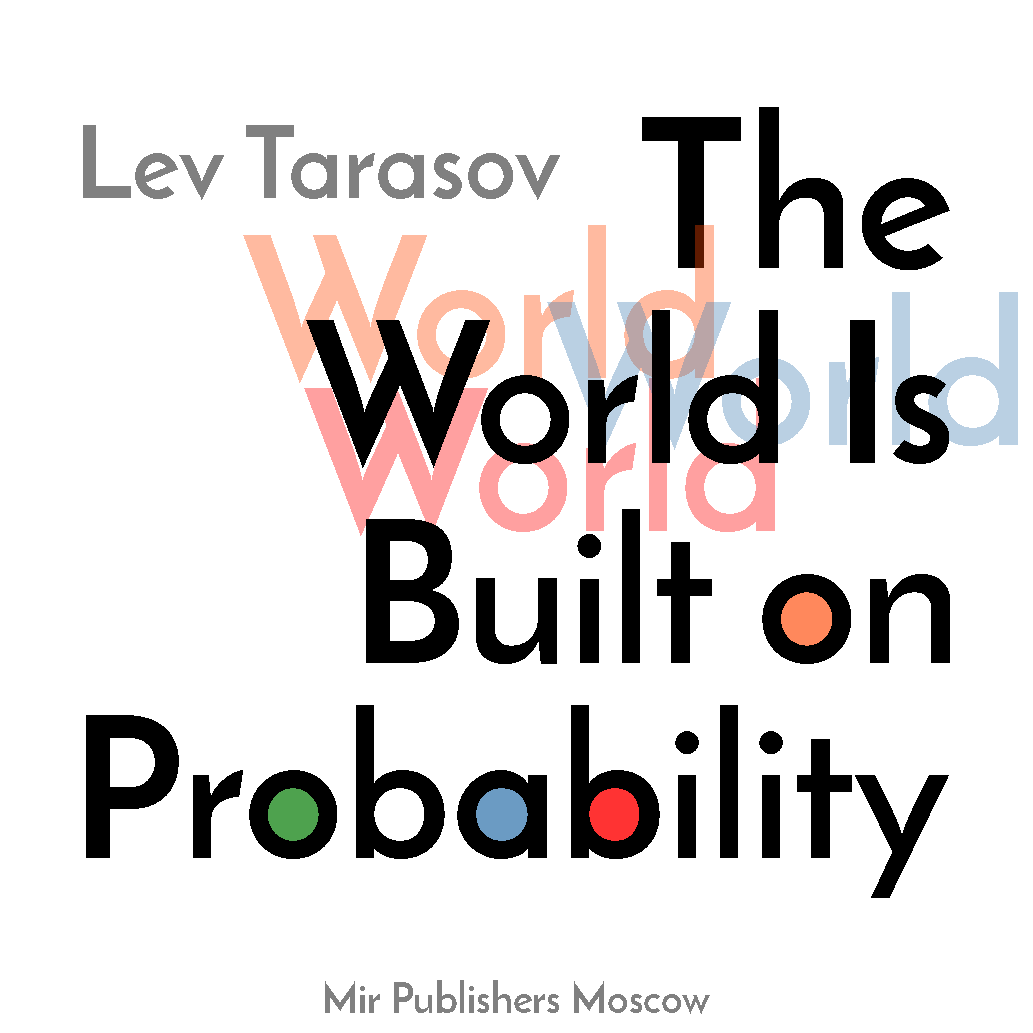
\includepdf{figures/twibop2fc.pdf}
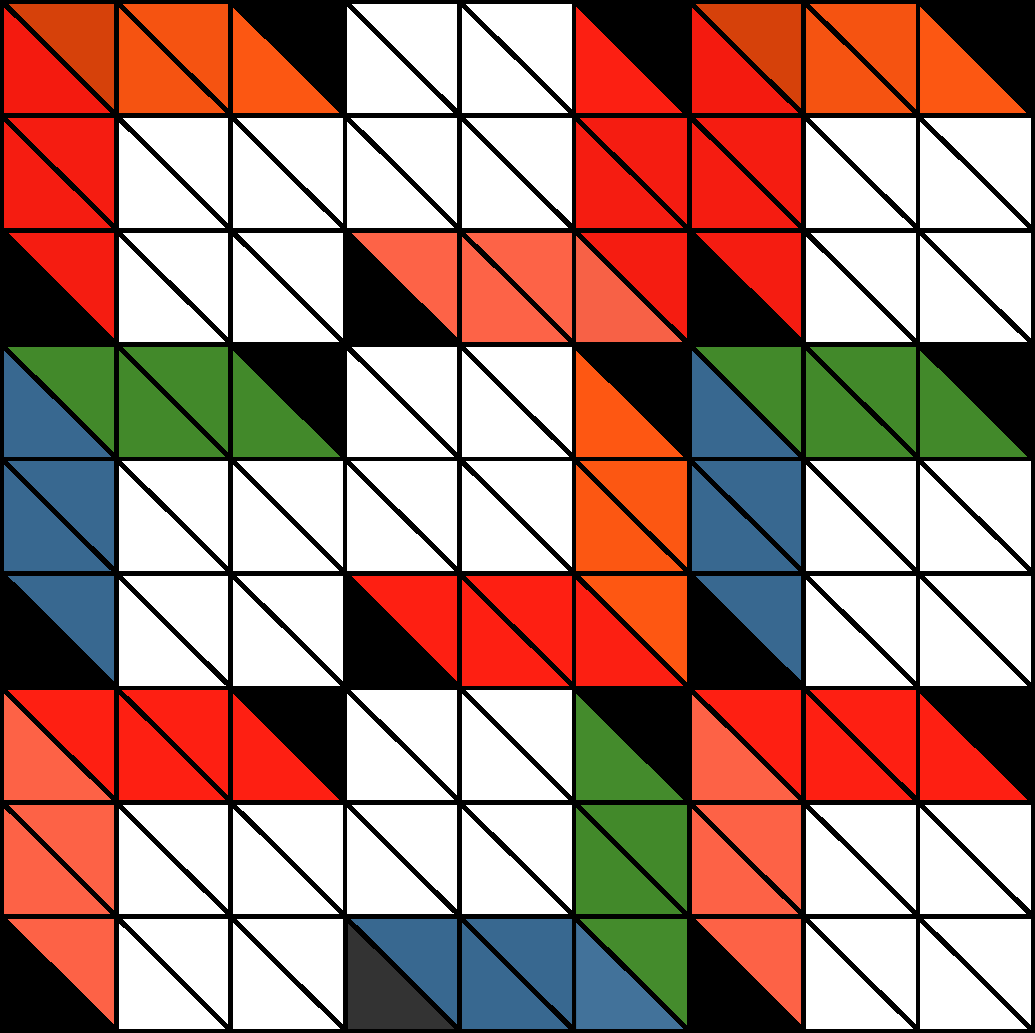
\includepdf{figures/twibopfj.pdf}
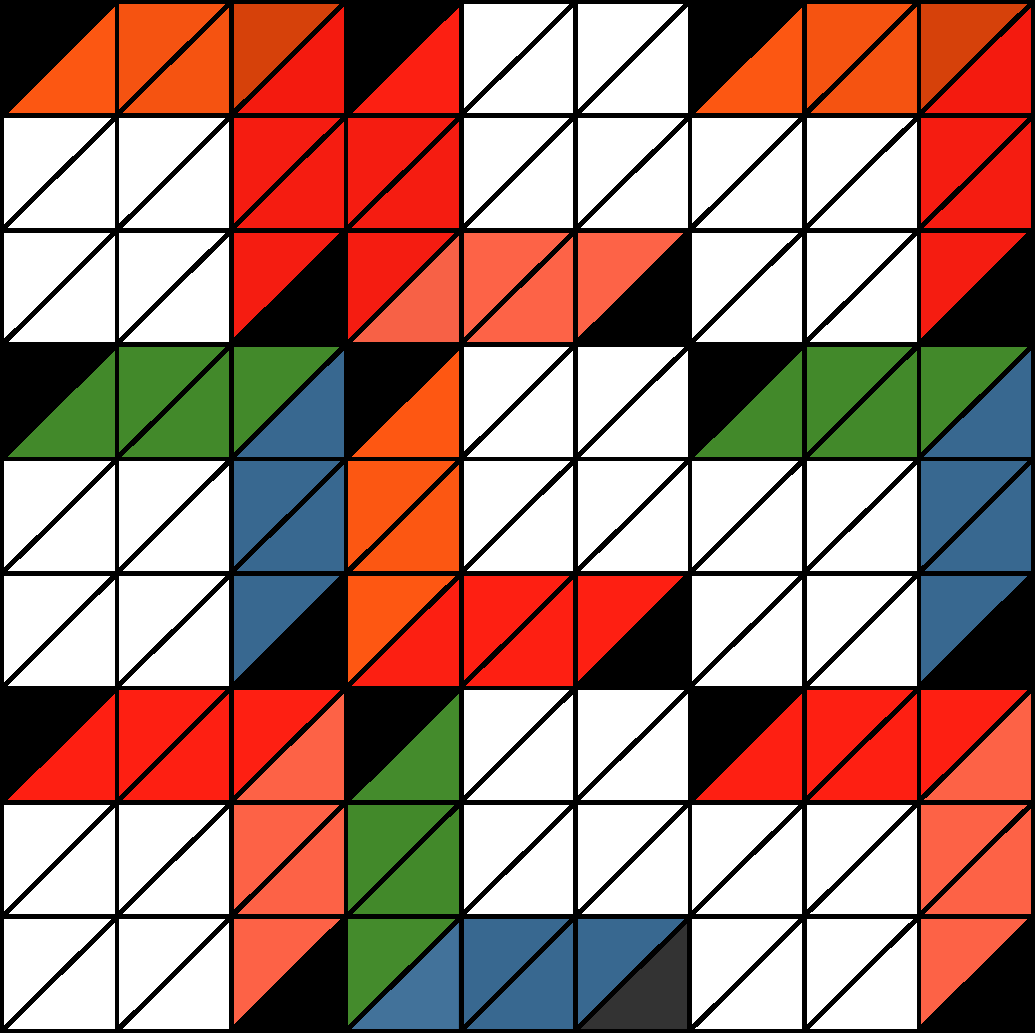
\includepdf{figures/twibopbj.pdf}

\cleardoublepage

\arrayrulecolor{gray} % <sets color of the \hline in tables
%\verbatimfontfamily{inconsolata}
\maketitle



%\begin{savequote}[0.55\linewidth]

%\newline
%\qauthor{F. Engels}
%\end{savequote}
% !TEX root = twibop2.tex
%\thispagestyle{empty}
%11.B. TapaCOB
%OCHOBbl
%KBAHTOBO MEXAHK
%HSA9.TanbCTBO Bwcwafl WKOna MOCKBa
\clearpage

\thispagestyle{empty}
\vspace*{2cm}
\begin{Huge}
\noindent
\textsf{ Lev Tarasov\\[1cm]
The World is Built \\ on Probability}\\[1cm]
\end{Huge}
%\vspace{3cm}
%\begin{large}
%\end{large}
\vspace{3.5cm}
\begin{center}
\begin{Large}
\textbf{MIR Publishers Moscow}
\end{Large}
\end{center}
\clearpage
\thispagestyle{empty}

%\cleardoublepageb
\noindent
\begin{smaller}

\begin{tcolorbox}{}
Translated from the Russian by \emph{Michael Burov}\\
First published 1988 \\
\noindent
Revised from the 1984 Russian edition \\

This completely digital version typeset in using \LaTeX{} with EB Garamond font by \\
\textsc{damitr mazanav} \url{damitr@proton.me} \\ 
Released on the web by \textcolor{CornflowerBlue}{\url{http://mirtitles.org}} in 2023.\\

Access the \LaTeX{} project files \url{gitlab.com/mirtitles/twibop}\\


\includegraphics[width=0.2\textwidth]{figures/cc-by-sa.pdf}\\

Creative Commons by SA 4.0 License\\
\end{tcolorbox}


\begin{tcolorbox}[title=About Mir Titles Project]

The Mir Titles project is an attempt to conserve the knowledge in the form of various books that came out during the Soviet era for the future generations. The collection contains books on science, mathematics, philosophy, popular science, history. The collection also has Soviet, Russian and children's literature. The project would not have been possible without the help we received from friends and contributors from across the world. 
\end{tcolorbox}


\begin{tcolorbox}[title=Foreword]

I am very happy to release this completely electronic version of one of my favourite books. In this electronic edition all the figures have been reworked in the SVG format using Inkscape for a clearer presentation.  in \LaTeX{}.
-- \textsc{damitr}
\end{tcolorbox}



\setcounter{tocdepth}{3}
\end{smaller}
\cleardoublepage
%\dominitoc


%\begin{savequote}[0.55\linewidth]

%\newline
%\qauthor{F. Engels}
%\end{savequote}


%%% Local Variables:
%%% mode: latex
%%% TeX-engine: xetex
%%% TeX-master: "tarasov-twibop"
%%% End:


\tableofcontents

% !TEX root = twibop2.tex


\chapter*{Preface}
\addcontentsline{toc}{chapter}{Preface}
\markboth{Preface}{Preface}
\label{ch-preface}

\epigraph{\ldots In nature, where chance also seems to reign, we have
  long ago demonstrated in each particular field the inherent
  necessity and regularity that asserts itself in this
  chance.}{F. Engels}



A vast concourse of events and phenomena occur in the world around
us. The events are interrelated: some are effects or outcomes of others
which are, in turn, the causes of still others. Gazing into this gigantic whirlpool of interrelated phenomena, we can come to two significant conclusions. One is that there are both completely determined (uniquely defined) outcomes and ambiguous outcomes. While the former can be precisely predicted, the latter can only be treated probabilistically. The second, no less essential conclusion is that ambiguous outcomes occur much more frequently than completely determined ones. Suppose you press a button and the lamp on your desk lights up. The second event (the lamp lights up) is the completely determined result of the first event (the button is pressed). Such an event is called a \redem{completely determined} one. Take another example: a die is tossed. Each face of the die has a different number of dots. The die falls and the face with four dots ends up at the top. The second event in this case (four dots face-up) is not the completely determined outcome of the first event (the die is tossed). The top face may have contained one, two, three, five, or six dots. The event of appearance of the number of dots on the top face after a die is tossed is an example of a \redem{random} event. These examples clearly indicate the
difference between random and completely determined events.


We encounter random events (and randomness of various kinds) very
often, much more frequently than is commonly thought. The choice of
the winning numbers in a lottery is random. The final score of a
football match is random. The number of sunny days at a given
geographical location varies randomly from year to year. A set of
random factors underlies the completion of any service activity:
delivery ambulance arrival, telephone connection, etc.

Maurice Glaymann and Tamas Varga have written an interesting book
called \redem{Les Probabilit\'es \`a l'\'ecole} (Probability in Games
and Entertainment), in which they make an interesting remark: 
\begin{quote}
``When facing a chance situation, small children think that it is possible to  \redem{predict} its outcome. When they are a bit older, the believe that  \redem{nothing can be postulated}. Little by little they discover that there are patterns hiding behind the seeming chaos of the random world, and these patterns can be used to get their bearings in
reality.''
\end{quote}
There are three distinct stages here: lack of understanding
of the random at first, then mere confusion, and finally a correct
viewpoint. Let us forget small children for a time and try to apply
this to ourselves. We shall have to recognize that frequently we stop
at the first stage in a simple-minded belief that any outcome can be
precisely predicted. The misconception that randomness is simply equal
to chaos, or the absence of causality, has lasted a long time. And
even now not everybody clearly appreciates that the abundance of
random events around us conceal definite (\redem{probabilistic})
patterns.

These ideas prompted me to write this book. I want to help
the reader discover for himself the probabilistic nature of the world
around us, to introduce random phenomena and processes, and to show
that it is possible to orient oneself in this random world and to
operate effectively within it.  

This book begins with a talk between myself and an imaginary reader
about the role of chance, and ends with another talk about the
relationship between randomness and symmetry. The text is divided into
two major parts. The first is on the concept of probability and
considers the various applications of probability in practice, namely,
making decisions in complicated situations, organizing queues,
participating in games, optimizing the control of various processes,
and doing random searches. The basic notions of cybernetics,
information theory, and such comparatively new fields as operations
research and the theory of games are given. The aim of the first part
is to convince the reader that the random world begins directly in his
own living room because, in fact, all modern life is based on
probabilistic methods. The second part shows how fundamental chance is
in Nature using the probabilistic laws of modern physics and biology
as examples. Elements of quantum mechanics are also involved, and this
allows me to demonstrate how probabilistic laws are basic to
microscopic phenomena. The idea was that by passing from the first
part of the book to the second one, the reader would see that
probability is not only around us but is at the basis of everything.

In conclusion I would like to express my gratitude to everyone who
helped me when writing this book. I.I. Gurevich, Corresponding
Member of the USSR Academy of Sciences, gave me the idea of writing this text and gave me a number of other provoking ideas concerning the material and structure of the book. B.V. Gnedenko, Member of the USSR Academy of Sciences, G.Ya. Myakishev, D.Sc. (Philosophy), and O.F. Kabardin. Cand. Sc. (Physics and Mathematics) read the manuscript thoroughly and made valuable remarks. V.A. Ezhiv and A.N. Tarasova rendered me constant advice and unstinting support the whole time I was preparing the text. 

\cleardoublepage


%%% Local Variables:
%%% mode: latex
%%% TeX-engine: xetex
%%% TeX-master: "tarasov-twibop"
%%% End:


\mainmatter

\part{Tamed Chance}
% !TEX root = twibop2.tex
\chapter*{Introduction}
\markboth{introduction}{introduction}
\label{ch-intro}

\epigraph{And chance, inventor God \ldots}{A. S. Pushkin}

\section*{A Discussion on the Role of Chance}


%{\setlength{\parindent}{0cm}
\begin{dialogue}
%\parindent{}
 \athr ``You wrote some nice words about chance in the Preface. In spite of them, I still think chance plays a negative role on the whole. Naturally, there is good luck, but everybody knows it is better not to count on it. Chance interferes with our plans, so it's better not hang on it, we should rather ward it off as much as possible.''

  \athr ``That is exactly the traditional attitude towards the random. However, it is an attitude we must clearly review. First of all, is it really possible to get by without the random?''

\rdr ``I don't say that it's possible. I said we should try.''

  \athr ``Suppose you work at an ambulance centre. Obviously, you cannot foresee when an ambulance will be needed, where it will be necessary to send it to, and how much time the patient will require. But a practical decision depends on all of these points. How many doctors should be on duty at anyone time? On the one hand, they should not be idle waiting for calls for long periods of time, yet on the other hand,  patients should not have to remain without aid for too long. You cannot avoid chance. What I am trying to say is: we cannot \redem{eliminate} chance, and so we must \redem{take} it \redem{into account}.''


\rdr ``True, we have to make peace with chance in this
  example. However, it still is a negative factor.''

\athr ``Thus, we see that sometimes we have to take
  chance into consideration rather than control it. But we can go
  further. We can discover situations in which chance becomes a
  positive factor rather than a negative one, so that it is desirable
  to raise the level of the random threshold.''

\rdr ``I don't understand you.''

\athr ``Of course, chance occasions interfere with our
  plans. At the same time because it makes us new solutions and
  improve our ability to create''.

\rdr ``Do you mean an improvement is obtained by
  overcoming difficulties?''

\athr  ``The main point is that randomness can create new
  possibilities. An American writer has written an interesting science
  fiction story. A group of scientists with various disciplines is officially
informed that a sensational discovery has been made, but unfortunately
the discoverer died in an explosion during a demonstration of the
phenomenon and thus the secret was lost. In reality neither the
invention nor the inventor ever existed. The scientists were presented
with the evidence of a tragedy: indistinct fragments of records, a
library, and an equipped laboratory. In other words, the scientists
were given a vast quantity of unconnected information with chance data
from various fields of science and technology. The evidence could be
called informational noise. The scientists were certain a discovery
had been made, and therefore the target was achievable. They utilized
all the information at their disposal and `revealed' the secret of the
non-existing invention. We might say that they succeeded in sifting information from the noise.''  

\rdr  ``But that's only a science fiction story.''  

\athr  ``True. However, the idea behind the story is far from being
fiction. Any discovery is related to the use of random factors.''  

\rdr  ``I don't think anyone can discover anything important
unless he or she has a professional grasp of the subject.''  

\athr  ``I think so too. Moreover, a discovery requires both
expertise on the part of the researcher and a certain level of the
development within the science as a whole. And yet \ldots, random factors
play a fundamental role in that.'' 

\rdr  ``As I understand, the word fundamental means something
primary, something at the basis. Can you apply the term fundamental to something random? I admit that randomness may be useful. But can it be fundamental? In the last analysis, we deal with random variables when there is something we do not know and cannot take into account. ''  

\athr  ``By believing that randomness is related to inadequate
knowledge, you make it \redem{subjective}. It follows that you believe that
randomness appears, as it were, on the surface and that there is
nothing random at the basis of phenomena. Is it correct?''  

\rdr  ``Precisely. That is why we cannot assert randomness is
fundamentality. As science develops, our ability to take different
factors into account increases, and the result is that the domain of
random variables will gradually recede. There is sense in saying that
 science is the enemy of chance. ''  

\athr ``You're not quite right. Indeed, the advance of
  science enhances our ability to make scientific predictions, that
  is, science is against the random factor. But at the same time, it
  turns out that while our scientific knowledge becomes deeper, or,
  more accurately, while we look at the molecular and atomic aspects
  of phenomena, randomness not only does not become less important,
  bit on the contrary, it reigns supreme. Its existence proves to be
  independent of the degree of our knowledge. Randomness reveals its
  \redem{fundametality} at the level of the microcosm.''

\rdr  ``This is the first time I've heard someone say
  that. Please tell me more.''

\athr  ``Let me say at once that this topic has had a long
  history. It was first formalized in Ancient Greece with two
  approaches to the random being stated. The two views are associated
  with the names of Democritus and Epicurus. Democritus identified the
  random with the \redem{unknown}, believing that Nature is completely
  deterministic. He said:  People have created an idol out of the
    random as a cover for their inability to think things out.
  Epicurus considered that the random is inherent in various
  phenomena, and that it is, therefore, \redem{objective}. Democritus's
  point of view was preferred for a long time, but in the $20^{\text{th}}$ century, the progress of science showed that Epicurus was right. In his doctoral thesis \redem{Difference Between the Democritian and Epicurian Philosophy on Nature} (1841), Karl Marx positively evaluated Epicurus's view of the random and pointed out the deep philosophical significance of the teachings of Epicurus on the  \redem{spontaneous}  displacement of atoms. Of course, we should not exaggerate the contribution of Epicurus to our understanding of the random because he could only guess.''

\rdr  ``It turns out that I presented Democritus's views
  on the random without knowing it. But I would like to have some
  concrete examples showing the fundamentality of the random.''

\athr  ``Consider, for instance, a nuclear-powered
  submarine. How is the engine started?'' 

\rdr  ``As far as I understand it, special
  neutron-absorbing rods are drawn from the core of the reactor. Then
  a controlled chain reaction involving the fission of uranium nuclei
  begins \ldots{}'' 

\athr ``(interrupting)  Let us try and see how everything begins.''

\rdr  ``After entering a uranium nucleus, a neutron triggers its
disintegration into two fragments and another neutron is released. The
neutrons split two more uranium nuclei; four neutrons are then set
free, which in turn split four more nuclei. The process develops like an avalanche.''

\athr  ``All right. But where does the first neutron come from?''

\rdr  ``Who knows? Say, they come from cosmic rays.''

\athr  ``The submarine is deep under water. The thick
  layer of water protects it from cosmic rays.''

\rdr  ``Well then, I don't know \ldots{}''

\athr   ``The fact is that a uranium nucleus may either
  split because a neutron enters it or it may decay
  \redem{spontaneously. The process of spontaneous nuclear fission is
    random.}''

\rdr ``But maybe spontaneous nuclear fission is caused
  by factors we do not know about yet.''

\athr  ``This is something physicists have been trying to
  solve. Many attempts have been made to find the  hidden
    parameters which govern the processes in the microcosm. It has
  been concluded that there are no such parameters, and therefore
  randomness in the microcosm is fundamental. This cornerstone problem
  is thoroughly treated in \redem{quantum mechanics}, a theory which
  appeared in the early $20^{\text{th}}$ century in connection with research
  on atomic processes.''

\rdr  ``The only thing I know about quantum mechanics is
  that it describes the laws governing the behaviour of elementary particles.''
  
\athr  ``We shall talk about quantum mechanics in more
  detail later. Let me only note here that it demonstrates the
  fundamental role of spontaneous processes and, therefore,
  demonstrates the fundamentality of the random. The operation of any
  radiation generator, from a vacuum tube to a laser, would be
  impossible without spontaneous processes. They are fundamental as
  the  trigger without which the radiation generation would not start.''

\rdr  ``And yet, it is difficult for me to believe that
  randomness is fundamental. You mentioned a nuclear-powered
  submarine. When the captain orders that the engines be turned on, he
  does not rely on a lucky chance. An appropriate button is pressed,
  and the engines start (if they are in good condition). The same can
  be said when a vacuum tube is turned on. Where is the randomness here?''

\athr  ``Nevertheless, when we consider phenomena in the
  microcosm, the processes are triggered by random factors.'' 

\rdr  ``However, we generally deal with processes
  occurring in the macrocosm.''

\athr  ``Firstly, while studying the world around us and
  trying to comprehend its \redem{cause and effect relations}, we must
  address the atomic level, i. e., the level of microcosm
  phenomena. Secondly, the randomness in microcosmic phenomena is
  essentially reflected in the processes observed at the macrocosmic scale.''
  
\rdr  ``Can you give me an example when the
  fundamentality of randomness reveals itself at the macrocosmic scale?''
  
\athr ``\redem{Evolution}, which is a continuous process in both
  the plant and animal kingdoms, may serve as an example. Evolution
  relies on mutation, i.e., random changes in the structure of
  genes. A random mutation may be rapidly spread by the reproduction
  of the organisms themselves. It is essential that selection occurs
  simultaneously with mutation. The organisms which contain the random
  gene are then selected to that those best fitted to their
  environment survive. In consequence, evolution requires the
  \redem{selection of random gene changes}.''

\rdr  ``I don't quite understand this business of
  selection.''
  
\athr ``Here's an example. The flowers of a certain
  orchid look like a female wasp. They are pollinated by male wasps
  which take the flowers to be females. Suppose a mutation occurs, and
  the shape and colour of the flower are changed. The flower will then
  remain unpollinated. The result is that the mutation is not passed
  on to the new generation. It may be said that selection rejected the
  mutation which changed the outward appearance of the flower. There
  was a species of orchid which became a self-pollinator, the flowers
  of this  species rapidly acquired diverse shape and colour owing to
  the mutation.''

\rdr  ``As far as I know, evolution progresses in the
  direction of the differentiation of species. Doesn't this show that
  the mutations underlying evolution are not, in fact, so random?''

\athr  ``That argument doesn't stand to reason. Evolution
  selects the fittest organisms rather than the more
  complex. Sometimes a higher degree of organization is preferable,
  but sometimes this is not the case. This is why human beings,
  jelly-fish, and the influenza virus can coexist in today's world. It
  is essential that evolution leads to the appearance of new species
  that are unpredictable in principle. It may be said that \redem{any species is unique because it occurred fundamentally} by chance.''

\rdr  ``I have to admit that the randomness does look to be
a fundamental factor indeed.''

\athr  ``Since we are discussing the fundamentality of
  randomness in the picture of evolution, let me draw your attention
  to one more important point. Modern science demonstrates that
  \redem{chance} and \redem{selection} are the `creator'.''

\rdr  ``Just as Pushkin said, `And chance, inventor God \ldots{}'''

\athr  ``Precisely. This line is strikingly accurate.''

\rdr  ``It appears that when speaking about chance and
  selection, we should imply the \redem{selection of information from noise}, shouldn't we? The same selection that we discussed in connection
  with the science-fiction story.''
  
\athr `` Absolutely.''

\rdr  ``I have to agree that we should consciously
  recognize the existence of randomness rather than try and control it.''

\athr  ``We could say more. Naturally, the randomness
  which is due to the incompleteness of our knowledge is
  undesirable. While studying the world, man has fought, is fighting,
  and will continue to fight it. It should be noted at the same time
  that there is an \redem{objective} randomness underlying every
  phenomena along with the \redem{subjective} randomness which is due
  to lack of data on a phenomenon. We should also take into account
  the positive, creative role of the random. And in this connection it
  is really necessary to recognize and control randomness. Man should
  be able, when necessary, to create special situations, abundant with
  the random, and utilize the situation to his own ends.''

\rdr  ``But is it really possible to treat randomness in
  such a way? Isn't it like trying \redem{to control the uncontrollable}?''

\athr   ``Both science and daily life indicate that it is
  possible to orient ourselves consciously in very random
  situations. Special calculation methods have been developed that
  depend on randomness. Special theories have been produced, such as
  \redem{queueing theory}, the \redem{theory of games}, and the
  \redem{theory of random search}, to deal with it.''

\rdr  ``It is hard for me to imagine a scientific theory
  built on randomness.''

\athr  ``Let me emphasize right away that randomness does
  not preclude scientific prediction. The fundamentality of randomness
  does not mean that the world around us is chaotic and devoid of
  order. Randomness does not imply there are no causal relations. But
  we shall deal with all that later. It is interesting to try and
  imagine a world in which randomness as an objective factor is
  \redem{completely absent}.''

\rdr  ``This would be an ideally ordered world.''

\athr ``In such a world, the state of any object at a
  given time would be unambiguously determined by its past states and,
  in its turn, would determine the future states just as
  definitely. The past would be strictly connected with the present,
  as would the present with the future.''

\rdr  ``Anything occurring in such a world would be
predetermined.''

\athr  ``Pierre Laplace, a great French scientist of the
  $17^{\text{th}}$ century, suggested in this connection that we imagine a superbeing who knew the past and the future of such a world in
  every detail. Laplace wrote:''  
  \begin{quote}
  `The intellect who could know, at a
    given moment, every force that animates the nature and the
    relative positions of its every component, and would, in addition,
    be vast enough to analyse these data, would describe by a single
    formula the motions of the greatest bodies in the universe and the
    motions of the lightest atoms. There would be nothing uncertain
    for this being, and the future, like the past, be open to his gaze.'
\end{quote}

\rdr  ``An ideally ordered world is therefore unreal.''

\athr  ``As you see, it isn't hard to feel that the real
  world should admit the existence of objective randomness. Now let us
  return to the problem of causal relations. These relations are
  \redem{probabilistic} in the real world. It is only in particular cases (for
  example, when solving maths problems at school) that we deal with
  unambiguous, strictly determined relations. Here we approach one of
  the most essential notions of the modern science, the notion of
  \redem{probability}.''

\rdr  ``I'm familiar with it. If I throw a die, I can
  equally expect any number of dots from one to six. The probability
  of each number is the same and equal to 1/6.''

\athr  ``Suppose you stand at the side of a road, with
  motor-cars passing by. What is the probability of the first two
  digits in their four digit number being equal?''

\rdr  ``The probability equals 1/10.''

\athr  ``Therefore, if you're patient and observe enough
  cars, about one tenth of them will have number-plates with the same
  first two digits, would they? Say, about thirty cars out of 300 will
  have such plates. Maybe, 27 or 32, but not 10 or 100.''

\rdr  ``I think so.''

\athr  ``But then there would be no need to stand at the roadside.
The result could be predicted. This is an example of \redem{probabilistic prediction}. Look at how many random factors are involved in this situation. A car could turn off the road before reaching the observer,
or another car could stop or even turn back. And nonetheless, both
today and tomorrow, about 30 cars out of 300 would have plates with
the same first two digits.''

\rdr ``So, in spite of numerous random factors, the
  situation has a certain constancy.''
  
\athr  ``This constancy is commonly called \redem{statistical
  stability}. It is essential that statistical stability is observed
  because of random factors rather than despite them.''

\rdr  ``I hadn't thought that we deal with probabilistic
  predictions everywhere. They include, for instance, sports
  predictions and weather forecasts.''

\athr  ``You're absolutely right. An important point is
  that probabilistic (statistical) causal relations are common, while
  those leading to unambiguous predictions are just a special
  case. While definite predictions only presuppose the necessity of a
  phenomenon, probabilistic predictions are related simultaneously
  both with necessity and randomness. Thus, mutations are random, but
  the process of selection is governed by laws, that is, it is a
  necessary prerequisite.''

\rdr  ``I see. The individual acts of the spontaneous
  fission of uranium nuclei are random, but the development of the
  chain reaction is unavoidable.''

\athr  ``Taken separately, any discovery is
  random. However, a situation which is favourable for the appearance
  of such a chance should exist. This chance is determined by the
  advance of science, the expertise of the researchers, and the level
  of measurement technology. A discovery is random, but the logic of
  the progress leading to the discovery in the long run is regular,
  unavoidable, and necessary.''

\rdr  ``Now I see why the fundamentality of randomness does not
result in the disorder of our world. Randomness and necessity are
always combined.''

\athr   ``Correct. Friedrich Engels wrote in \redem{The
    Origin of the Family, Private Property, and the State} (1884):
   `In Nature, where chance also seems to reign, we have long ago
    demonstrated in each particular field the inherent necessity and
    regularity that asserts itself in this chance.' The Hungarian
    mathematician A.R\'enyi wrote about the same thing in an
    interesting book \redem{Letters on Probability}'':  
    \begin{quote}
    `I came across \redem{Contemplations} by
    Aurelius and accidentally opened the page where he wrote about two
    possibilities: the world is either in vast chaos or, otherwise,
    order and regularity reign supreme. And although I had read these
    lines many times, it was the first time that I thought over why
    Marcus Aurelius believed that the world should be dominated by
    either chance or order. Why did he believe that these two
    possibilities are contradictory? The world is dominated by
    randomness, but order and regularity operate at the same time,
    being shaped out of the mass of random events according to the
    laws of the random.'
	\end{quote}
\rdr  ``As far as I understand, order and regularity are
  produced from a mass of random events, and this leads to the concept
  probability.
''
\athr  ``You're absolutely right. \redem{Individual factors} vary
  from case to case. At the same time, the \redem{picture as a whole} remains
  stable. This stability is expressed in terms of \redem{probability}. This is
  why our world proves to be flexible, dynamic, and capable of advancing.''

\rdr  ``It follows that the world around us may justly be
  said to be a world of probability.''

\athr  ``It is better to speak of the \redem{world as being
    built on probability}. When we examine this world, we shall
  concentrate on two groups of questions. Firstly, I shall show how
  man, owing to his use of probability in science and technology, was
  able to  tame randomness and thus turn it from being his enemy
  into an ally and friend. Secondly, using the achievements of modern
  physics and biology, I shall demonstrate the probabilistic features
  of the laws of nature. In consequence, I shall show that the world
  around us (including both the natural and artificial world) is
  really built on probability.''
  
\end{dialogue}
\cleardoublepage

%%% Local Variables:
%%% mode: latex
%%% TeX-engine: xetex
%%% TeX-master: "tarasov-twibop"
%%% End:

% !TEX root = twibop2.tex

\chapter{Mathematics of Randomness}
\epigraph{This doctrine, combining the accuracy of mathematical proofs
  and the uncertainty of chance occasions and making peace between
  these seemingly contradictory elements has a full right to contend
  for the title of the mathematics of the random.}{Blaise Pascal}

\section{Probability} 

\txthead{Classical definition of probability.} When
we toss a coin, we do not know which will land face up, heads or
tails. However, there is something we do know. We know that the
chances of both heads and tails are equal. We also know that the
chances of any of the faces of a die landing face up are equal. That
the chances are equal in both examples is due to \redem{symmetry}. Both the
coin and the die are symmetrical. When two or more events have equal
chances of occurring, we call them equally possible outcomes. Heads or
tails are \redem{equally possible} outcomes. Suppose we are interested in a
certain result while throwing a die, for instance, a face with a
number of dots exactly divisible by three. Let us call outcomes
satisfying such a requirement \redem{favourable}. There are two favourable
outcomes in our example, namely, a three or a six. Now let us call
outcomes \redem{exclusive} if the appearance of one in single trial makes it
impossible for the others to appear at the same trial. A die cannot
land with several faces up, so they are exclusive outcomes.  

We can now formulate the classical definition of probability: 
\begin{mybox}{}
The probability of an event is the ratio of the number of favourable outcomes to the total number of equally possible exclusive outcomes.
\end{mybox}

Suppose $P_{A}$ is the probability of an even $A$, $m_{A}$ is the
number of favourable outcomes, and $n$ the total number of equally
possible and exclusive outcomes. According to the classical definition
of probability 
\begin{equation}%
P_{A} = \dfrac{m_{A}}{n}.
\label{eq-1.1}
\end{equation}
If $m_{A} =n$, then $P_{A}= 1$ and the event $A$ is a \redem{certain}
event (it always occurs in every outcome). If $m_{A} =0 $, then $P_{A}
=0$, and the event $A$ is an \redem{impossible} event (it never
occurs). The probability of a \redem{random} event lies between $0$ and
$1$. 

Let an event $A$ be throwing a die and getting a number exactly
divisible by three. Here $m_{A} = 2$ and so the probability of the
event is 1/3, because $n=6$. Consider one more example. We have a
bag with 15 identical but differently coloured balls (seven white, two green, and six
red). You draw a ball at random. What is the probability of drawing
a white (red or green) ball? Drawing a white ball can be regarded as an
event $A$, drawing a red ball is an event $B$, and drawing a green ball is an event $C$. The number of favourable outcomes of drawing a ball of
a certain colour equals the number of balls of this colour, i. e., $m_{A} = 7$, $m_{B} = 6$, and $m_{C} = 2$. Using (\ref{eq-1.1}) and given $n = 15$, we can find the
probabilities:
\begin{equation*}
P_{A} = \dfrac{m_{A}}{n} = \dfrac{7}{15}, \quad P_{B} =
\dfrac{m_{B}}{n} = \dfrac{2}{15}, \quad P_{C} = \dfrac{m_{C}}{n} = \dfrac{2}{15}. 
\end{equation*}

\txthead{Addition and multiplication of probabilities.} What is the probability that a randomly drawn ball will be either red or green? The number of favourable outcomes is $m_{B} + m_{C} = 6 + 2 = 8$, and therefore the probability will be
\begin{equation*}%
P_{B+C} = \frac{m_{B}+m_{C}}{n} = \frac{8}{15}.
\end{equation*} 
We see that $ P_{B+C} = P_{B} + P_{C} $. The probability of drawing either a red or a green ball is the sum of two probabilities: the probability of drawing a red ball and that of drawing a green ball. The probability of drawing a ball which is either red or green or white is the sum of three probabilities, $P_{A} + P_{B} + P_{C}$. It is equal to unity $(7/15 + 2/5 + 2/15 = 1)$. This stands to reason because the event in question will always occur.

The rule for adding probabilities can be formulated as follows: 
\begin{mybox}{}
The probability of one event of several exclusive events occurring is the sum of the probabilities of each separate event.
\end{mybox}

\newcolumntype{g}{>{\columncolor{LightYellow}}c}
%\begin{table}[ht]

\begin{wrapfigure}{O}{\mfwidth}
\begin{footnotesize}
\centering
\setlength\arrayrulewidth{1.25pt}\arrayrulecolor{Tomato}
\begin{tabular}{gggggg}
\hline
%&col1 &col2 &col3 &col4 & col5 &col6 &col7\\
%\hline
% row1& \ra & \ra & \ra & \ra & \ra & \ra & \ra \\
% row2& \ra & \ra & \ra & \ra & \ra & \ra & \ra \\
% row3& \ra & \ra & \ra & \ra & \ra & \ra & \ra \\
% row4& \ra & \ra & \ra & \ra & \ra & \ra & \ra \\
% row5& \ra & \ra & \ra & \ra & \ra & \ra & \ra \\
% row6& \ra & \ra & \ra & \ra & \ra & \ra & \ra \\
\cellcolor[gray]{0.8}(1,1) & (2,1) & (3,1) & (4,1) & (5,1) & (6,1) \\
(1,2) & \cellcolor[gray]{0.8}(2,2) & (3,2) & (4,2) & (5,2) & (6,2) \\
(1,3) & (2,3) & \cellcolor[gray]{0.8}(3,3) & (4,3) & (5,3) & (6,3) \\
(1,4) & (2,4) & (3,4) & \cellcolor[gray]{0.8}(4,4) & (5,4) & (6,4) \\
(1,5) & (2,5) & (3,5) & (4,5) & \cellcolor[gray]{0.8}(5,5) & (6,5) \\
(1,6) & (2,6) & (3,6) & (4,6) & (5,6) & \cellcolor[gray]{0.8}(6,6) \\
\hline
\end{tabular}
\caption{Possible outcomes of rolling a die.\label{die-table}}
\end{footnotesize}
%fig 1.1
\end{wrapfigure}

Suppose that two dice are thrown. What is the probability of getting
two fours at the same time? The total number of equally possible
exclusive outcomes is $n = 6 \times 6 = 36$. Each one is listed in \figr{die-table}, where the left figure in the parentheses is the number on one die, and the right figure is the number on the other. There is only one favourable outcome, and it is indicated in \figr{die-table} as (4,4). Hence, the probability of the event is 1/36. This probability is the product of two probabilities: the probability of a four appearing on one die and that of a four on
the other i.e. 
\begin{equation*}%
P_{44} = P_{4} \times P_{4} = \frac{1}{6} \times \frac{1}{6} = \frac{1}{36}.
\end{equation*}

The rule for multiplication of probabilities can be formulated as
follows:
\begin{mybox}{}
The probability of several events occurring simultaneously equals the product of the probabilities of each separate event.
\end{mybox}
By the was, it is not necessary for the events to be simultaneous. Instead of throwing two dice at the same time, we could throw a
 single die twice. The probability of getting two fours at the same
 time when two dice are thrown is the same as the probability of
 getting two fours when one die is thrown twice.

\begin{figure}
 \centering
 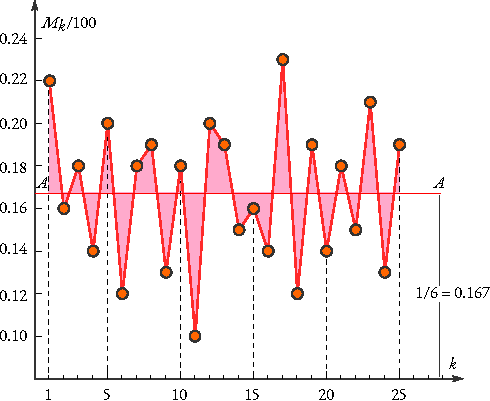
\includegraphics[width=0.9\tfwidth]{figures/die-graph.pdf}
\caption{Outcomes of rolling a dice many times.\label{die-graph}}
%fig 1.2
\end{figure}
 
 
In many cases both rules (addition and multiplication of
probabilities) are used jointly to calculate the probability of an
event. Suppose we are interested in the probability $P$ of the \redem{same} number coming up on two dice. Since it is only essential that the numbers be equal, we can apply the rule for adding probabilities,
\begin{equation*}
P = P_{11} + P_{22} + P_{33} + P_{44} + P_{55} + P_{66}.
\end{equation*}
Each of the probabilities $P_{ii}$ is, in turn, a product $P_{i} \times P_{i}$. \redem{Hence}
\begin{equation*}
P = (P_{1} \times P_{1}) + (P_{2} \times P_{2}) + \ldots + (P_{6}
\times P_{6}) = 6 \left( \dfrac{1}{6} \times \dfrac{1}{6} \right) = \dfrac{1}{6}.
\end{equation*}
This result can be obtained right away from \figr{die-table}, where
the favourable outcomes are shown in the gray, (1,1), (2,2), (3,3),
(4,4), (5,5), and (6,6). The total number of such outcomes is six. Consequently, $P = 6/36 = 1/6$.

\txthead{Frequency and probability.} The classical
definition of probability and the rules for addition and
multiplication of probabilities can be used to calculate the
probability of a random event. However, what is the practical value of
such calculations? For instance, what does it mean in practice that
the probability of getting a four when a die is thrown equals 1/6? Naturally, the assertion does not imply that a four will appear once and only once in any six trials. It is possible that it will appear once, but it is also possible that it will appear two (or more) times, or that it will not appear at all. In order to discover the probability of an event in practice we should perform a large number of trials and calculate how frequently a four appears.


Let us perform several sets of trials, for instance, throwing the die
100 times in each set. Let us designate $M_{1}$ to be the number of
times a four appears in the first set, $M_{2}$ to be the
number of fours in the second set, etc. The ratios
$M_{1}/100, M_{2}/100, M_{3}/100, \ldots{} $ are the frequencies with
which a four appeared in each set. Having performed several sets of
trials, we can see that the frequency of the appearance of a four
\redem{varies from set to set in a random fashion in the vicinity of
  the probability} of the trials, we can see that the frequency of the
appearance of a four \redem{varies} from set to set \redem{in a random
  fashion in the vicinity of the probability} of the given event,
i.e. in the vicinity of 1/6. This is clear from \figr{die-graph}, where the number $k$ of sets of trials is plotted along the abscissa axis and the frequencies with which a four appears along
the axis of ordinates. 

\begin{figure}%[ht]
 \centering
 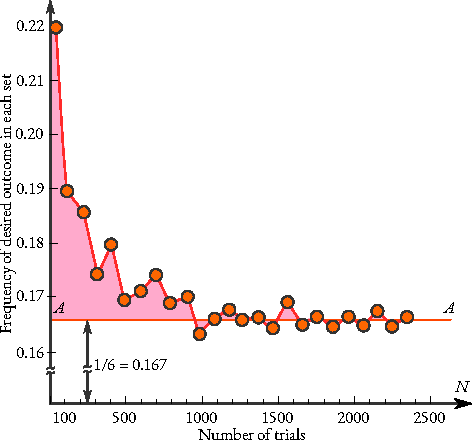
\includegraphics[width=0.9\tfwidth]{figures/die-graph2.pdf}
\caption{Frequencies of outcomes of trials of a die as a function of number of trials. Note how the deviation of the frequency of the occurrence of an event from its probability decreases as the number of trials increases.\label{die-graph2}}
 \end{figure}
 
Naturally, if we perform the experiment again,
we will get other values of the frequencies $M_{k}/100$. However, the
pattern of oscillations of the frequencies of the event under
consideration will be stable: the deviations upwards and downwards
from the straight line $AA$, which is associated with the probability
of the event, will balance. Even though the amplitudes of the
deviations will vary from set to set, they will not tend to grow or
decrease. This is a consequence of the \redem{equivalence} of each set
of trials. The number of trials in each set is the same, and the
results obtained in a given set do not depend on the results in any
other set.


 

Let us make an important change in that we gradually increase the
number of trials in each set. Using the results of our previous
experiment, as presented in \figr{die-graph}, let us obtain a new
result by \redem{adding} the value of a set of trials to the result of
the preceding sets. In other words, we calculate the number of fours
in the first 100 trials (in our case, $M_{1} = 22$), then the number of
fours in the first 200 trials $(M_{1} + M_{2} = 22 + 16 = 38)$, the in
the first 300 trials  $(M_{1} + M_{2} +  M_{3}  = 22 + 16 + 18 = 56)$
etc. We then find the frequencies of getting a four in the each new
set: $M_{1}/100 = 0.22$, $(M_{1} + M_{2} )/200 = 0.19$, $(M_{1} +
M_{2} +  M_{3})/300  = 0.187$, etc.  These frequencies are plotted in
\figr{die-graph2} against the number of trials in each set (100,
200, \ldots, 2500). The figure demonstrates a crucial fact: the
deviation of the frequency of the occurrence of an event from its
probability decreases as the number of trials increases. In other
words, 
\begin{mybox}{}
frequency of the occurrence of a random event tends to its probability with increasing number of trials.
\end{mybox}




\txthead{Is it possible to give a definition of probability based on frequency?}
Since the frequency of the occurrence of a random event tends to its
probability as the number of trials increases, we might well ask whether
we can define the probability of an event as the limit of the ratio of the
number of its occurrence to the number of trials as the number of trials
lends to infinity. Suppose $N$ is the number of trials and $M_{A} (N)$ is the
number of occurrence of an event A. We want to know whether we can
define the probability $P_{A}$ of the event $A$ as

\begin{equation}
P_{A} = \lim_{N \rightarrow \infty}  \left[ \frac{M_{A} (N)}{N}
\right].
\label{eq-1.2}
\end{equation}

Richard von Mises (1883-1953), a German mathematician of the early
20th century, believed that equation \eqref{eq-1.2} could be considered
a definition of the probability of a random event, and he called it
the \redem{frequency} definition of probability. Von Mises pointed out
that the classical definition of probability \eqref{eq-1.1}
only ``works'' when there is a \redem{finite} number of \redem{equally}
possible outcomes. For instance, situations involving the throwing of
coins or dice.


However, we often encounter situations without the \redem{symmetry}
that determines whether the outcomes are equally possible. These are
the cases when we cannot apply the classical definition of
probability. Von Mises assumed that then the frequency definition can
be used because it does not require a finite number of equally
possible outcomes and, moreover, does not require any calculation of
probability at all.  A probability using the frequency approach is
determined by experiment rather than being calculated.


However, is it possible to determine the probability of a random event
in practice using \eqref{eq-1.2}? The relationship
presupposes an \redem{infinite} number of identical trials. In
practice, we must stop at a \redem{finite} number of trials, and it is
debatable what number to stop at. Should we stop after a hundred
trials, or is it necessary for there to be a thousand, a million, or a
hundred million? And what is the accuracy of the probability
determined in such a way? There are no answers to these questions.
Bcsides, it is not practicable to provide the same conditions while
performing a very large number of trials, to say nothing of the fact
that the trials may be impossible to repeat.


Consequently, relationship \eqref{eq-1.2} is practically
useless, moreover it is possible to prove (though I shall not do so)
that the limit in \eqref{eq-1.2} \redem{does not} strictly
speaking \redem{exist}. This means that the Von Mises's error was that
he made an unwarranted generalization from a correct proposition: he
concluded that the probability of a random even is the limit of the
frequency of its occurrence when the  number of trials tends to
infinity from the correct observation that the frequency of the
occurrence of a random even approaches its probability as the number
of trials increases. 

\txthead{Geometrical definition of probability.}
Suppose that two people have agreed to meet at a certain place between
nine and ten o'clock. They also agreed that each would wait for a
quarter of an hour and, if the other didn't arrive, would leave. What
is the probability that they meet?  Suppose $x$ is the moment one
person arrives at the appointed place, and $y$ is the moment the other
arrives. Let us consider a point with coordinates $(x, y)$ on a plane
as an outcome of the rendezvous. Every possible outcome is within the
area of a square each side of which corresponds to one hour ( Figure
\ref{prob-meeting}). The outcome is favourable (the two meet) for all
points $(x, y)$ such that $\vert \, x - y \, \vert \le 1/4$. These
points are within the blue part of the square in the \figr{prob-meeting}. 
  
  \begin{figure}[ht]
 \centering
 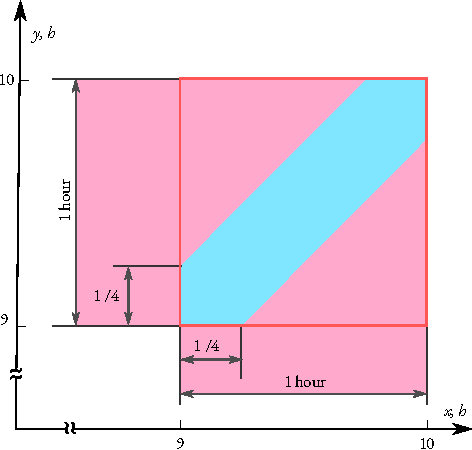
\includegraphics[width=0.9\tfwidth]{figures/prob-meeting.pdf}
\caption{Finding the probability using the geometrical method.\label{prob-meeting}}
%fig 1.4
 \end{figure}
  
  All the outcomes are exclusive
and equally possible, and therefore the probability of the rendezvous
equals the ratio of the blue area to the area of the square. This
is reminiscent of the ratio of favourable outcomes to the total number
of equally possible outcomes in the classical definition of
probability. It should be borne in mind that this is a case where the
number of outcomes (both favourable and unfavourable) is
infinite. Therefore, instead of calculating the ratio of the number of
favourable outcomes to the total number of outcomes, it is better to
consider here the ratio of the area containing favourable outcomes to
the total area of the random events.




It is not difficult to use \figr{prob-meeting} and find the
favourable area; it is the difference between the area of the whole
square and the unhatched area, i.e. $1 - \left( 3/4 \right)^2 =
7/16 \, h^{2}$. Dividing $7/16 \, h^{2}$ by $1\, h^{2}$, we find the probability of the rendezvous to be 7/16.

This example illustrates the geometrical definition of probability:
\begin{mybox}{}
The probability of a random event is the ratio of the area favourable for an
event to the total area of events.
\end{mybox}
The geometrical definition of probability is a generalization of the classical definition for the case when the number of equally possible outcomes is infinite.


\txthead{The development of the concept of
    probability.} Although probabilistic notions were used by ancient
Greek philosophers (such as Democritus, Epicurus, and Carus
Lucretius), the theory of probability as a science began in the
mid-$17^{\text{th}}$ century, with the work of the French scientists Blaise
Pascal and Pierre Fermat and the Dutch scientist Christian
Huygens. The classical definition for the probability of a random
event was formulated by the Swiss mathematician Jacob Bernoulli in
\redem{Ars conjectandi} (The Art of Conjectures). The definition was
given its final shape later by Pierre Laplace. The geometrical
definition of probability was first applied in the $18^{\text{th}}$
century. Important contributions to probability theory were made by
the Russian mathematical school in the $19^{\text{th}}$ century (P.L. Chebyshev,
A.A. Markov, and A.M. Lyapunov). 

The extensive employment of probabilistic concepts in physics and technology demonstrated, by the early $20^{\text{th}}$ century, that there was a need for a more refined definition of probability. It was necessary, in particular, in order
to eliminate the reliance of probability on ``common sense''.  An
unsuccessful attempt to give a general definition for the probability
of a random event on the basis of the limit of its frequency of
occurrence was made, as we have seen, by Richard von Mises.  However,
an \redem{axiomatic} approach rather than a frequency one resulted in more
refined definition of probability. The new approach was based on a
set of certain assumptions (axioms) from which all the other
propositions are deduced using clearly formulated rules.  


The \redem{axiomatic} definition of probability now generally accepted was
elaborated by the Soviet mathematician A.N. Kolmogorov, Member of the
USSR Academy of Sciences, in \redem{The Basic Notions of the Probability
Theory} (1936, in Russian). I shall not discuss the axiomatic
definition of probability because it would require set theory. Let me
only remark that Kolmogorov's axioms gave a strict mathematical
substantiation to the concept of probability and made probability
theory a fully fledged mathematical discipline.  

The existence of several definitions for the same notion (probability)
should not worry the reader.

As L.E. Maistrov put it in \redem{The Development of the Notion of
  Probability} (Nauka, Moscow, 1980): 
\begin{quote}
  ``There are many definitions of 
notions, and this is an essential feature of modern science. Hence the
notion of probability is no exception. Modern definitions in science
represent diverse viewpoints, of which there may be very many for a
fundamental notion, and each view reflects a property of the defined
notion. This includes the notion of probability.'' 
\end{quote}
Let me add that new
definitions for a notion appear as our understanding of it becomes
deeper and its properties are made clearer.


\section{Random Numbers}
\txthead{Random Number Generators.}
 Let us put ten identical balls numbered
from 0 to 9 into a box. We take out a ball at random and write down
its number. Suppose it is five. Then we put the ball back into the box,
stir the balls well, and take out a ball at random. Suppose this time we
get a one. We write it down, put the ball back into the box, stir the
balls, and take out a ball at random again. This time we get a two.
Repeating this procedure many times, we obtain a disordered set of
numbers, for instance: 5, 1, 2, 7, 2, 3, 0, 2, 1, 3, 9, 2, 4, 4, 1, 3, \ldots{} This sequence is disordered because each number appeared \redem{at random}, since
each time a ball was taken out at random from a well-stirred set of
identical balls.


Having obtained a set of random digits, we can compile a set of
random numbers. Let us consider, for instance, four-digit numbers. We
need only separate our series of random numbers into groups of four
digits and consider each group to be a random number: 5127, 2302,
1392, 4413, \ldots{}

Any device that yields random numbers is called a \redem{random number
generator}. There are three types of generators: \redem{urns},
\redem{dice}, and \redem{roulettes} (\figr{random-generators}). Our box with balls is an urn.

Dice are the simplest random number generators. An example of such
a generator is a cube each of whose faces is marked with a different
number. Another example is a coin (or a token). Suppose five of the
faces of a cube are marked with the numbers 0, 1, 2, 3, 4, while the sixth
face is unmarked. Now suppose we have a token one side of which is
labelled with 0 and the other with 5. Let us throw the cube and token
simultaneously and add together the numbers that appear face up, the
trial being discounted when the unmarked face lands face up. This
generator allows us to obtain a disordered set of numbers from 0 to 9,
which can then be easily used to produce sets of random numbers.
A roulette is a circle marked in sectors, each of which is marked with
a different number. A roulette has a rotating arrow or rolling ball.
A trial involves spinning the arrow and recording the number

A roulette is a circle marked in sectors, each of which is marked with
a different number. A roulette has a rotating arrow or rolling ball.
A trial involves spinning the arrow and recording the number
corresponding to the sector of the roulette circle within which the arrow
stops.

Note that a roulette may have any number of sectors. For instance.
we could divide a circle into ten sectors and label them from 0 to 9. As
a random number generator, our roulette in this case is equivalent to
the two generators discussed above: 
\begin{enumerate}[leftmargin=1cm,label=(\arabic*),noitemsep,nolistsep]
\item an urn with ten balls and
\item a die and a token thrown at the same time.
\end{enumerate}
A diagram of these equivalent random number generators is shown in \figr{random-generators}.

\begin{figure}[!ht]
 \centering
 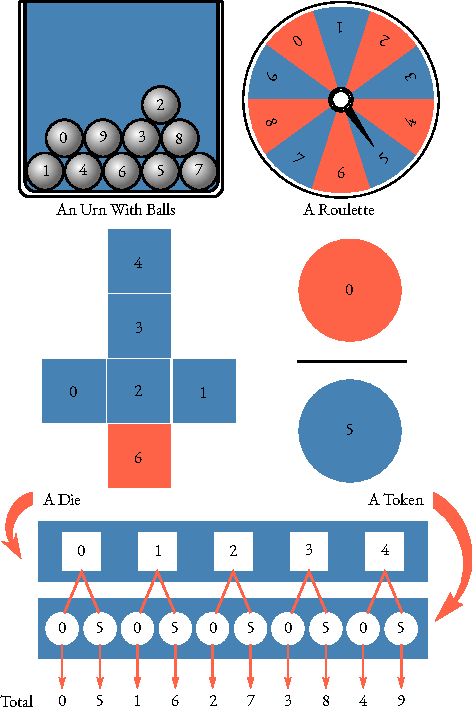
\includegraphics[width=0.82\tfwidth]{figures/random-generators.pdf}
\caption{Three types of random number generators: urns, dice and roulettes.
\label{random-generators}}
 \end{figure}
%\clearpage
\txthead{Tables of Random Numbers.} An example of a random number table is
shown in Figure \ref{random-table}. The table consists of three hundred four-digit
numbers. Each digit in the table was chosen randomly, as a result of
a trial, e.g. throwing a die and a token. Therefore, it is understandable
that there is no order in the numbers, and there is no way of predicting
which digit will follow a given one. You could compile many tables after
many trials. Nevertheless, there will not be even the shadow of order in
the sequence of digits.

%\newcolumntype{g}{>{\columncolor{LightYellow}}c}
%\begin{table}[ht]
\begin{figure}[!ht]
\centering
\setlength\arrayrulewidth{1pt}\arrayrulecolor{Tomato}
\renewcommand{\arraystretch}{.9}
\begin{footnotesize}
\begin{tabular}{cccccccccc}
\hline
%&col1 &col2 &col3 &col4 & col5 &col6 &col7\\
%\hline
%\hline
0655 & 8453 & 4467 & 3234 & 5320 & 0709 & 2523 & 9224 & 6271 & 2607 \\
\rowcolor{lightgray}5255 & 5161 & 4889 & 7429 & 4647 & 4331 & 0010 & 8144 & 8638 & 0307 \\
6314 & 8951 & 2335 & 0174 & 6993 & 6157 & 0063 & 6006 & 1736 & 3775 \\
\rowcolor{lightgray} 3157 & 9764 & 4862 & 5848 & 6919 & 3135 & 2837 & 9910 & 7791 & 8941 \\
9052 & 9565 & 4635 & 0653 & 2254 & 5704 & 8865 & 2627 & 7959 & 3682 \\
\hline
4105 & 4105 & 3187 & 4312 & 1596 & 9403 & 6859 & 7802 & 3180 & 4499 \\
\rowcolor{lightgray}1437 & 2851 & 6727 & 5580 & 0368 & 4746 & 0604 & 7956 & 2304 & 8417 \\
4064 & 4171 & 7013 & 4631 & 8288 & 4785 & 6560 & 8851 & 9928 & 2439 \\
\rowcolor{lightgray} 1037 & 5765 & 1562 & 9869 & 0756 & 5761 & 6346 & 5392 & 2986 & 2018 \\
5718 & 8791 & 0754 & 2222 & 2013 & 0830 & 0927 & 0466 & 7526 & 6610 \\
\hline
5127 & 2302 & 1392 & 4413 & 9651 & 8922 & 1023 & 6265 & 7877 & 4733 \\
\rowcolor{lightgray} 9401 & 2423 & 6301 & 2611 & 0650 & 0400 & 5998 & 1863 & 9182 & 9032 \\
4064 & 5228 & 4153 & 2544 & 4125 & 9654 & 6380 & 6650 & 8567 & 5045 \\
\rowcolor{lightgray} 5458 & 1402 & 9849 & 9886 & 5579 & 4171 & 9844 & 0159 & 2260 & 1314 \\
2461 & 3497 & 9785 & 5678 & 4471 & 2873 & 3724 & 8900 & 7852 & 5843 \\
\hline
4320 & 4553 & 2545 & 4436 & 9265 & 6675 & 7989 & 5592 & 3759 & 3431 \\
\rowcolor{lightgray} 3466 & 8269 & 9926 & 7429 & 7516 & 1126 & 6345 & 4576 & 5059 & 7746 \\
9313 & 7489 & 2464 & 2575 & 9284 & 1787 & 2391 & 4245 & 5618 & 0146 \\
\rowcolor{lightgray} 5179 & 8081 & 3361 & 0109 & 7730 & 6256 & 1303 & 6503 & 4081 & 4754 \\
3010 & 5081 & 3300 & 9979 & 1970 & 6279 & 6307 & 7935 & 4977 & 0501 \\
\hline
9599 & 9828 & 8740 & 6666 & 6692 & 5590 & 2455 & 3963 & 6463 & 1609 \\
\rowcolor{lightgray} 4242 & 3961 & 6247 & 4911 & 7264 & 0247 & 0583 & 7679 & 7942 & 2482 \\
3585 & 9123 & 5014 & 6328 & 9659 & 1863 & 0532 & 6313 & 3199 & 7619 \\
\rowcolor{lightgray} 5950 & 3384 & 0276 & 4503 & 3333 & 8967 & 3382 & 3016 & 0639 & 2007 \\
8462 & 3145 & 6582 & 8605 & 7300 & 6298 & 6673 & 6406 & 5951 & 7427 \\
\hline
0456 & 0944 & 3058 & 2545 & 3756 & 2436 & 2408 & 4477 & 5707 & 5441 \\
\rowcolor{lightgray} 0672 & 1281 & 8897 & 5409 & 0653 & 5519 & 9720 & 0111 & 4745 & 7979 \\
5163 & 9690 & 0413 & 3043 & 1014 & 0226 & 5460 & 2835 & 3294 & 3674 \\
\rowcolor{lightgray} 4995 & 9115 & 5273 & 1293 & 7894 & 9050 & 1378 & 2220 & 3756 & 9795 \\
6751 & 6447 & 4991 & 6458 & 9307 & 3371 & 3243 & 2958 & 4738 & 3996 \\
\hline
\end{tabular}
\end{footnotesize}
\caption{A table of random numbers.\label{random-table}}
\end{figure}

This is not amazing. A chance is a chance. But a chance has a reverse
aspect. For instance, try and count how many times each digit occurs in \figr{random-table}. You will find that digit 0 occurs 118 times (the frequency it
appears is $118/1200 = 0.099$), digit 1 occurs 110 times (the frequency it
appears is 0.090), digit 2 occurs 114 times (0.095), digit 3 occurs 125
times (0.104), digit 4 occurs 135 times (0.113), digit 5 occurs 135 times
(0.113), digit 6 occurs 132 times (0.110), digit 7 occurs 116 times (0097),
digit 8 occurs 93 times (0.078), and digit 9 occurs 122 times (0.102). We
can see that the appearance frequency for each digit is about the same,
i. e. close to 0.1. Naturally, the reader has come to a conclusion that 0.1
is the \redem{probability} that a digit appears. The reader may say that the
appearance frequency of a digit is close to the probability of its
appearance over a long series of trials (there are 1200 trials here).

Although this is natural, we should wonder once (again how an
unordered set of \redem{random} digits can have an \redem{inherent stability}. This is a demonstration of the reverse aspect of chance and illustrates the
determinism of \redem{probability}.

I advise the reader to ``work'' a little with a random number table (see
\figr{random-table}). For instance, 32 numbers out of the three hundred ones in the table begin with zero, 20 begin with 1, 33 begin with 2, 33 begin with 3,
38 begin with 4, 34 begin with 5, 34 begin with 6, 24 begin with 7, 20
begin with 8, and 32 begin with 9. The probability that a number begins
with a certain digit equals 0.1. It is easy to see that the results of our
count are in a rather good keeping with this probability (one tenth of
three hundred is thirty). However, the deviations are more noticeable
than in the example considered earlier. But this is natural because the
number of trials above was 1200 while here it is much less, only 300.

It is also interesting to count how many times a digit occurs in the
second place (the number of hundreds), in the third place (tens), and the
fourth place (units). It is easy to see that in every case the frequency
with which a given digit appears is close to the probability, i.e. close to
0.1. Thus, zero occurs in the second place 25 times, in the third place 33
times, and in the fourth place 28 times.

An example with the number-plates of motor-cars randomly passing
the observer was cited in the introduction. It was noted that the
probability that the first two digits in the licence number were identical
is 0.1. The probability that the two last digits of the number or two
middle digits or the first and the last digit are identical is the same.



In order to see this, we need not observe a sequence of cars passing
by. We can simply use a random number table (see \figr{random-table}). The four-digit random numbers in the table can be taken as the license numbers
of cars randomly passing the observer. We can see that 40 of the 300
number's have the same two first digits, 28 numbers have the same two
last digits, 24 numbers have the same two middle digits, and 32
numbers have the same first and last digits. In other words, the
frequencies with which a pair of identical digits appears actually
varies around the probability, i.e. in the neighbourhood of 0.1.




\section{Random Events}

When we throw a die or take a ball out of an urn we deal with
a \redem{random event}. There are several interesting problems where the
probability of a random event is required to be found.

\begin{wrapfigure}{O}{\mfwidth}
 \centering
 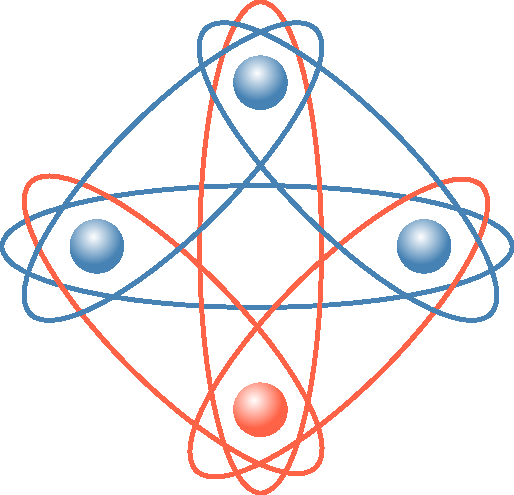
\includegraphics[width=\linewidth]{figures/three-balls.pdf}
\caption{Different ways of taking out two out of three blue and one
  red balls.\label{three-balls}}
\end{wrapfigure}


\txthead{A problem with coloured balls.} There are three blue balls and a red
ball in a box. You take two balls out of the box at random. Which is
more probable: that the two balls are blue or that one is blue and one is
red?

People often answer that it is more probable that two blue balls are
taken out because the number of blue balls in the box is three times
greater than the number of red ones. However, the probability of taking
out two blue balls is \redem{equal} to the probability of taking out a blue and
a red ball. You can see this by considering \figr{three-balls}. Clearly there are three ways in which two blue balls may be chosen and three ways of
choosing a blue and a red ball at the same time. Therefore, the
outcomes are equally probable.


We can also calculate the probability of the outcomes. The
probability of taking out two blue balls equals the product of two
probabilities. The first one is the probability of taking out a blue ball
from a set of four balls (three blue ones plus a red one), which is 3/4.
The second probability is that of taking out a blue ball from a set of
three balls (two blue ones plus a red one) which is 2/3. Consequently,
the probability of taking out two blue balls simultaneously is $3/4 \times
2/3 = 1/2$.

The probability of taking out a blue and a red ball is the sum $P_{\text{br}} +
P_{\text{rb}}$, where $P_{\text{br}}$, is the probability of taking out a blue ball from a set of four balls (three blue ones plus a red one) multiplied by the probability of taking out a red ball from a set of three balls (two blue ones plus it red one) and $P_{\text{rb}}$, is the probability of taking out a red ball from a set of four balls (the second all in this case must then be a blue one). In other words, $P_{\text{br}}$ is the probability of taking out a blue ball first and then a red ball while $P_{\text{rb}}$ is the probability of taking out a red ball first and then a blue ball. Inasmuch as $P_{\text{br}} = 3/4 \times 1/3 = 1/4$ and $P_{\text{rb}} = 1/4$, the probability of taking out a pair of differently coloured balls equals $1/4 + 1/4 = 1/2$. 

%\input{figures/fig-10}


\txthead{Throwing A Die: A Game.}  There are two players in this game, player
$A$ and player $B$. The die is thrown three times in succession during each
turn. If a certain face turns up at least once during a turn (let it be a 5),
player $A$ scores a point. But if the five does not turn up, a point is
scored by player $B$. The game is played until one of them scores, say,
a hundred points. Who has the chance of winning greater? Player $A$ or
player $B$?

In order to answer, we first calculate the probability of player
$A$ scoring a point in a turn (the die is thrown three times in succession).
He receives a point in any of the following three cases: if five turns up
in the first trial, if five does not turn up in the first trial but turns up in
the second one, and if five does not turn up in the first two trials but
turns up in the third one. Let us designate the probability of these three
events as $P_{1},  P_{2}$, and $P_{3}$, respectively. The sought probability is $P =
P_{1} + P_{2} + P_{3}$. Note that the probability of five appearing when the die
is thrown is {1/6}, and the probability that five does not appear is {5/6}. It
is clear that $P_{1} = 1/6$. To find $P_{2}$, we should multiply the probability of
the absence of a five in the first trial by the probability of its presence in
the second trial, $P_{2} = 5/6 \times 1/6 = 5/36$. The probability $P_{3}$ is the
product of the probability of the absence of a five in two trials (the first
and the second) and the probability of a five in the third trial, $P_{3}=
(5/6)^{2} \times 1/6 = 25/216$.  Consequently, $ P = P_{1} + P_{2} + P_{3} = 1/6 +
5/6 + 25/216 = 91/216$. Since $P < 1/2$, player $B$ has more chance of
winning this game. We could have reached the same conclusion in
a simpler way by considering the probability of player $B$ scoring a point
after three trials. This is the probability of the absence of five in three
trials: $p = 5/6 \times 5/6 \times 5/6 = 125/216$. Since $p> 1/2$, player $B$'s chances
are better. Note that $P+p=91/216+125/216=1$. This is natural
because one of the players, $A$ or $B$, must score a point in each turn.

Let us change the rules of the game a little: the die is thrown four
times rather than three times in each turn. The other conditions remain
the same. The probability of player $B$ scoring a point in a turn is
$5/6 \times  5/6 \times 5/6 \times 5/6 =625/1296$. This is less than $1/2$, and therefore now $A$ has a better chance of winning a game.



\txthead{The Problem Of An Astrologer.} A tyrant got angry with an astrologer
and ordered his execution. However, at the last moment the tyrant made
up his mind to give the astrologer a chance to save himself. He took
two black and two white balls and told the astrologer to put them into
two urns at random. The executioner was to choose an urn and pick
a ball out of it at random. If the ball was white, the astrologer would be
pardoned, and if the ball was black, he would be executed. How should
the astrologer distribute the balls between the two urns in order to give
himself the greatest chance of being saved?

\begin{figure}[!ht]
 \centering
 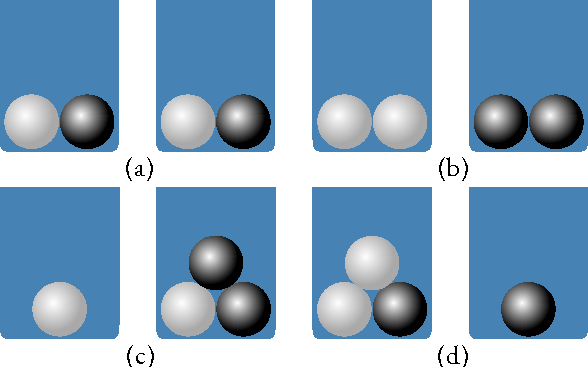
\includegraphics[width=0.75\tfwidth]{figures/ball-picking.pdf}
\caption{Different ways of arranging two white and two black balls for
  different probabilities of drawing out a ball of a given colour.\label{ball-picking}}
 \end{figure}

Suppose the astrologer puts a white and a black ball into each urn
(\figr{ball-picking}~\drkgry{(a)}). In this case, no matter which urn the executioner chooses, he will draw a white ball out of it with a probability of 1/2. Therefore, the probability the astrologer would be saved is 1/2.

The probability of the astrologer being saved will be the same if he
puts the two white balls into one urn and the two black balls into the
other (\figr{ball-picking}~\drkgry{(b)}). His destiny will be decided by the executioner when he chooses an urn. The executioner may choose either urn with equal probability.

The best solution for the astrologer is to put a white ball into one um
and a white ball and two black ones into the other urn (\figr{ball-picking}~\drkgry{(c)}). If the executioner chooses the first urn, the astrologer will certainly be saved, but if the executioner picks the second urn, the astrologer will be saved with a probability of {1/3}. Since the executioner chooses either urn with probability {1/2}, the overall probability that the astrologer will be saved is $(1/2 \times 1)+(1/2 \times 1/3)=2/3$.

By contrast, if the astrologer puts a black ball into one urn and
a black ball and two white balls into the other (\figr{ball-picking}~\drkgry{(d)}), the probability of him being saved will be smallest: $(1/2 \times 0)+(1/2 \times 2/3) = 1/3$.

Thus, in order to have the greatest chance of being saved, the
astrologer should distribute the balls between the urns as shown in
(\figr{ball-picking}~\drkgry{(c)}) This is the best strategy. The worst
strategy is to distribute the balls as shown in (\figr{ball-picking}~\drkgry{(d)}). Of course, the selection of the best strategy does not guarantee the desired outcome. Although the risk is decreased, it still remains.

\txthead{Wandering In A Labyrinth.} A labyrinth with treasure has a
death trap, as shown in \figr{labyrinth}. Unlucky treasure-hunters
die in the trap. What is the Probability that they will avoid the trap
and reach the treasure?
\begin{wrapfigure}[22]{O}{\mfwidth}
 \centering
 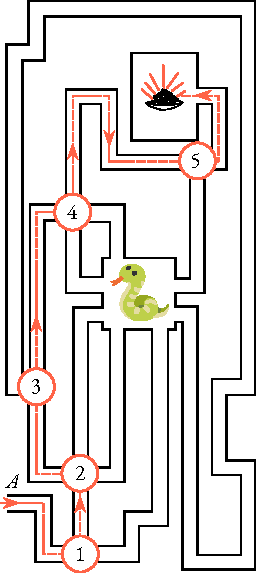
\includegraphics[width=0.9\linewidth]{figures/labyrinth.pdf}
\caption{The probability of finding the treasure or a trap in a labyrinth.\label{labyrinth}}
 \end{wrapfigure}
 
After walking away from the entrance $A$ to point {1} (see \figr{labyrinth}) a treasure-hunter may either go straight ahead (in
which case he walks directly into the trap) or turn to the left (in
which case he arrives at point {2}) We shall suppose he picks
either path at random, with equal probability, i.e. with probability
{1/2}. Alter arriving at point {2}, the treasure-hunter may
either go straight ahead or turn right or turn left with probability
{1/3}. The first two paths lead to the trap, while the third path
leads to point {3}. The probability of someone getting from the
entrance $A$ to point {3} is the product of the probability of
turning left at point {1} and the probability of turning left at
point {2}, i.e., $1 /2 \times 1/3$. It is easy to see now that the
probability of reaching point {4} from $A$ is
$1/2 \times 1/3 \times 1/2$; the probability of reaching point {5}
from $A$ is $1/2 \times 1/3 \times 1/2 \times 1/3$; and finally, the
probability of reaching the treasure from $A$ is
$P^{\,+} = 1/2 \times 1/3 \times 1/2 \times 1/3 \times 1/2 = 1/72$. The
only way of getting from the entrance of the labyrinth to the treasure
is shown in the figure by the dash line. The probability that a person
will follow it is thus $P^{\,+} = 1/72$, while the probability of
walking into the trap is $P^{\,-} = 71/72$.




The probability $P^{\,-}$ was calculated from the fact that $P^{\,+} +
P^{\,-} = 1$.  However, we can calculate $P^{\,-}$ directly. Let us expand
$P^{\,-}$ as the sum $P^{\,-} = P_{1} + P_{2} + P_{3} + P_{4} + P_{5}$ where the $P_{i}$ are
  the probabilities of arriving at point $i$ from $A$ multiplied by the
  probability of walking into the trap from point $i \,\, (i = 1, 2, 3, 4,
  5)$.
\begin{align*}
P_{1} & = 1/2, \\
P_{2} &= 1/2 \times 2/3, \\
P_{3} &= 1/2 \times 1/3 \times 1/2,\\
P_{4} &= 1/2 \times  1/3 \times 1/2 \times 2/3,\\
P_{5} & = 1/2 \times 1/3 \times 1/2 \times 1/3 \times 1/2.
\end{align*}
You can then find that $ P_{1} + P_{2} + P_{3} + P_{4} + P_{5} = 71/72$.

\section{Discrete Random Variables}

\txthead{Random Variables.}  Suppose there is a batch of {100}
manufactured articles and {11} articles are rejected as defective, {9}
articles are rejected in another batch of the same size, {10} articles
are rejected in the third one, {12} articles are rejected in the fourth
one, etc. We use $n$ to denote the overall number of manufactured
articles in a batch and $m$ to denote the number of rejected
articles. The number $n$ is constant (here $n = 100$) while the value of $m$
varies from batch to batch in a random manner. Suppose there is a
\redem{definite probability} that there will be $m$ rejected articles in a
randomly selected batch of $n$ articles.  


The number of rejected articles (the variable $m$) is an example of a
\redem{random variable}. \redem{It varies randomly from one trial to
  another, and a certain probability is associated with the occurrence
  of each value of the variable}. Note that we are dealing with a
discrete random variable here, i.e. it may only take a discrete set of
values (the integers from {0} to {100} in this case).

There are also \redem{continuous} random variables. For instance, the
length and weight of newborn babies vary randomly from child to child
and may take any value within a particular interval There are some
special features of continuous random variables which we shall discuss
later; we shall first consider discrete variables.


\txthead{Expected values and variance of a discrete random variable.}
Let $x$ be a discrete random variable which may assume $s$ values: $x_{1}, x_{2},
\ldots x_{m},  \ldots x_{s} $. These values are associated with the probabilities  $p_{1}, p_{2},
\ldots p_{m},  \ldots p_{s} $. For instance, $p_{m}$ is the probability that a variable is $x_{m}$. The sum of all the probabilities $( p_{1} + p_{2} +  \ldots + p_{s})$ is the probability that a trial will give one of the values  $x_{1}, x_{2},  \ldots x_{s} $, (without saying which one). This probability is unity. Consequently,
\begin{equation}%
\sum_{m=1}^{s} \, p_{m}= 1,
\label{eq-1.3}
\end{equation}
\footnote{The notation $\displaystyle \sum_{m=1}^{s}$ means that the summation is performed over all $m$ from 1 to $s$.}
The set of probabilities $p_{1} + p_{2} + \ldots + p_{s}$ (also called
the distribution of the probabilities) contains all the information
needed about the random variable. However, we do not need all the
probabilities for many practical purposes. It is sufficient to know two
most important characteristics of a random variable: its expected
value (its mathematical expectation) and its variance.

The \redem{expected value} is an average value of the random variable taken over a large number of trials. We shall use the letter $E$ to denote the expected value. The expected value of a random variable $x$ is the sum of the products of each variable and its probability, i.e.
\begin{equation*}%
E(x) =  p_{1}x_{1} +  p_{2}x_{2} +  \ldots +  p_{s}x_{s},
\end{equation*}
or using the summation sign,
\begin{equation}%
E(x) = \sum_{m=1}^{s} \, p_{m} \,x_{m}.
\label{eq-1.4}
\end{equation}
We also need to know how a variable deviates from the expected
value, or, in other words, how much the random variable is \redem{scattered}.
The expected value of the deviation from the expected value (that is the
difference $x - E(x)$) cannot be used because it is equal to zero. We can
show this as follows:
\begin{align*}%
E(x- E(x)) & =  \sum_{m=1}^{s} \, p_{m} \, ( x_{m} - E(x)), \\
& =  \sum_{m=1}^{s} \, p_{m} \,x_{m} - E(x) \,  \sum_{m=1}^{s} \,
  p_{m}, \\
& = E(x) - E(x),\\
& = 0.
\end{align*}
This is why the expected value of the \redem{squared} deviation (rather than the expected value of the deviation itself) is used, i.e.
\begin{equation}%
\textrm{var} = \sigma^{2} = E(x — E(x))^{2} = \sum_{m=1}^{s} \, p_{m}
\, ( x_{m} - E(x))^{2}.
\label{eq-1.5}
\end{equation}
This is the variance of a random variable and we shall use var to denote
it. The square root of the variable $\sqrt{\textrm{var}}$ is called the \redem{standard} (or
\redem{root-mean-square) deviation} $\sigma$ of the random variable. It is easy to show that
\begin{equation}
\textrm{var} = E (x^{2}) - (E(x))^{2}. 
\label{eq-1.6}
\end{equation}
Indeed,
\begin{align*}%
 \sum_{m=1}^{s} \, p_{m}  \, ( x_{m} - E(x))^{2} & =  \sum_{m=1}^{s} \, p_{m}
\, ( x_{m}^{2} - 2x_{m} E(x) + E(x))^{2}),\\
& = \sum_{m=1}^{s} \, p_{m}  \,  x_{m}^{2} - 2E(x) \sum_{m=1}^{s} \, p_{m}
\,  x_{m} + (E(x))^{2} \sum_{m=1}^{s} \, p_{m}, \\
& = E(x^{2}) - 2 E(x) E(x) + (E(x))^2,\\
& = E(x^{2}) - (E(x))^{2}.
\end{align*}


\begin{figure}[!h]
 \centering
 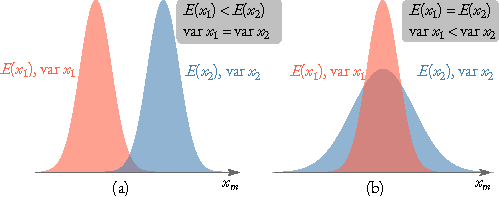
\includegraphics[width=\tfwidth]{figures/exp-val-variation.pdf}
\caption{Distributions of random variables with different
  parameters. (a) shows two distributions with different expected
  values but the same variance, while (b) shows two distributions with
  different variance but the same expected values.\label{exp-val-variation}}
 \end{figure}

Two probability distributions are shown in \figr{exp-val-variation}~\drkgry{(a)}. The two random variables possess different expected values while having the same
variance. Looking at \figr{exp-val-variation}~\drkgry{(b)}, we can see a different
picture: the random variables possess different variances while having
the same expected values.


\txthead{Bernoulli's Binomial Distribution.}  Suppose a series of $n$
independent identical trials is performed. The trials are independent
in the sense that the results of any trial do not influence the
results of any other trial. Some trials produce a desired outcome
while the rest do not. Let us call the desired outcome, ``event
$U$". This is a random event. Suppose event $U$ occurs in in trials. This
is a random variable. Let us consider the probability $P_{n}\,(m)$ that event
$U$ will occur $m$ times in a series of $n$ trials.


This is a commonly occurring situation. Suppose $n$ manufactured
articles are checked. Then event $U$ is a rejection, and $P_{n}\,(m)$ is
the probability of in articles being rejected out of a set of in
articles Suppose a hospital registers $n$ newborn babies and the event
$U$ is the birth of a girl. Hence $P_{n}\,(m)$ is the probability that
there will be $m$ girls in a set of $n$ newborn babies. Suppose in a
lottery, $n$ tickets are checked, event $U$ is the discovery of a
prize-winning ticket, and $P_{n}\,(m)$ is the probability that $m$
prize-winning tickets will be found out of a total of $n$
tickets. Suppose in a physics experiment $n$ neutrons are recorded,
the event $U$ is the occurrence of a neutron with an energy within a
certain range, and $P_{n}\,(m)$ is the probability that $m$ of the $n$
neutrons will possess energies in the range. In all these examples,
the probability  $P_{n}\,(m)$ is described by the same formula which is the
\redem{binomial distribution} (sometimes named after a $17^{\text{th}}$ century Swiss mathematician called Jacob Bernoulli).

The binomial distribution is derived by assuming that the probability
that event $U$ will occur in a single trial is known and does not vary
from trial to trial. Let us call this probability $p$. The probability that
event $U$ does not occur in a single trial is $q= 1 - p$. It is important that
the probability that an article is rejected does not depend in any way on
how many rejected articles there are in the given batch. The probability
that a girl is born in any actual delivery does not depend on whether
a girl or a boy was born in the previous birth (nor on how many girls
have so far been born). The probability of winning a prize neither
increases nor decreases as the lottery tickets are checked. The
probability that a neutron has an energy in a given range does not
change during the experiment.

Now, \redem{once the probability $p$ that a certain random event will occur in
a single trial is known, we find the probability $P_{n}(m)$ of $m$ occurrences in
a series of $n$ independent identical trials.}

Suppose the event $U$ occurred in the first $m$ trials but did not occur in
$n - m$ trials, then the probability of the situation would be $p^{m}q^{n-m}$.
Naturally, other orders are possible. For instance, event $U$ may not
occur in the first $n - m$ trials and occur in the rest in trials. The
probability of this situation is also $p^{m}q^{n-m}$. There are also other possible situations. There are as many situations as there are ways choosing
$n$ elements taken in at a time (this is written $\begin{psmallmatrix}n \\ m \end{psmallmatrix}$). The probability of each situation is identical and equals  $p^{m}q^{n-m}$. The order in which event $U$ occurs is inessential. It is only essential that it occurs in $m$ trials and does not occur in the remaining $n - m$ trials. The sought probability $P_{n}(m)$ is the sum of the probabilities of each $\begin{psmallmatrix}n \\ m \end{psmallmatrix}$ situation, i.e. the
product of  $p^{m}q^{n-m}$ and $\begin{psmallmatrix}n \\ m \end{psmallmatrix}$:
\begin{equation}%
P_{n}(m) = \mqty(n \\ m) \, p^{m}q^{n-m}.
\label{eq-1.7}
\end{equation}
There is a formula for the number of combinations of $n$ elements taken
$m$ at a time:
\begin{equation}%
\mqty(n \\ m)
= \frac{n!}{m! (n-m)!}
 = \frac{n(n-1)(n-2)\ldots (n-m+1)}{m!}.
\label{eq-1.8}
\end{equation}
Here $n! = 1 \cdot 2 \cdot 3 \cdot \ldots  \cdot n$ (read $n!$ as ``en factorial''), by convention $0 ! = 1$.

Substituting (\ref{eq-1.8}) into (\ref{eq-1.7}), we can find
\begin{equation}%
P_{n}(m) = \frac{n!}{m! (n-m)!} \, p^{m}q^{n-m}.
\label{eq-1.9}
\end{equation}
This is the \redem{binomial distribution}, or the distribution of a binomial
random variable. I shall explain this term below, and we shall see that
\begin{equation}%
\sum_{m=0}^{n}  P_{n}\,(m) = 1.
\label{eq-1.10}
\end{equation}


\begin{figure}[!h]
 \centering
 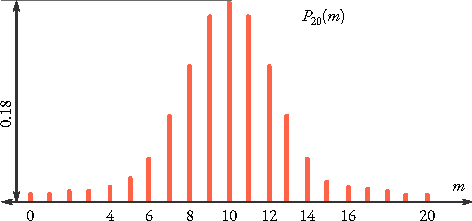
\includegraphics[width=0.8\tfwidth]{figures/binomial-dist.pdf}
\caption{The binomial distribution. \label{binomial-dist}}
 \end{figure}


By way of example, let us calculate the probability that $m$ girls are
born in a group of 20 babies. Assume that the probability of delivering
a girl is 1/2, We set $p= 1/2$ and $n = 20$ in expression \eqref{eq-1.9} and consider the integer values of variable $m$ within the range from 0 to 20. The result can be conveniently presented as a diagram (\figr{binomial-dist}). We see that the birth of 10 girls is the most probable; the probability of delivering, for instance, 6 or 14 girls is six times smaller.

If a random variable has a binomial distribution, then its expected
value is
\begin{equation*}
E(m) = \sum_{m=0}^{n} m \, P_{n}(m).
\end{equation*}
or the product of the number of trials and the probability of the event
in a single trial,
\begin{equation}%
E(m) = np.
\label{eq-1.11}
\end{equation}
The variance of such a random variable is the product of the number of
trials, the probability of the occurrence of the event in a single trial, and
the probability it does not occur:
\begin{equation}%
\textrm{var} = E(m^{2}) - (E(m))^2 = npq.
\label{eq-1.12}
\end{equation}


\txthead{The normal (Gaussian) Distribution.} Probability calculations using the
binomial distribution are difficult for large $n$. For instance, in order to
find the probability that 30 girls were delivered from 50 births, you have
to calculate
\begin{equation*}
P_{30}(50) = \frac{50!}{30!20!} (0.5)^{50}.
\end{equation*}
Note that even $20!$ is a 19—digit number. In such cases one can use a
formula which is the limit of the binomial distribution at large $n$:
\begin{equation}%
P_{n}\,(m) = \frac{1}{\sqrt{2 \pi \, \textrm{var}}} \exp \left( -  \frac{(m - E(m))^{2}}{2 \, \textrm{var}}  \right),
\label{eq-1.13}
\end{equation}
where $E\,(m) = np$ and $\textrm{var} = npq$, and $\exp = 2.718 \ldots$
is the base of natural logarithms. The distribution defined in
(\ref{eq-1.13}) is called the \redem{normal} or \redem{Gaussian distribution}.


\txthead{The Poisson Distribution.} If the probability that an event will
occur in a single trial is very small ($p \ll1$), the binomial distribution at
large $n$  becomes the \redem{Poisson} (rather than the normal) distribution, and is defined as
\begin{equation}%
P_{n}\,(m) = \frac{(np)^{m}}{m!} \exp (-np).
\label{eq-1.14}
\end{equation}
This distribution is also sometimes called the \redem{law of rare events}. It is
interesting to note that the variance of a random variable with
the Poisson distribution equals its expected value.

Two distributions are compared in \figr{poisson-gaussian}. The parameters of the
first distribution are $n = 30$ and $p = 0.3$, and it is close to the normal
distribution with the expected value $E\, (m) = 9$. The second distribution’s
parameters are $n = 30$ and $p = 0.05$, and it is close to the Poisson
distribution with $E\,(m)= 1.5$.

\begin{figure}[!h]
 \centering
 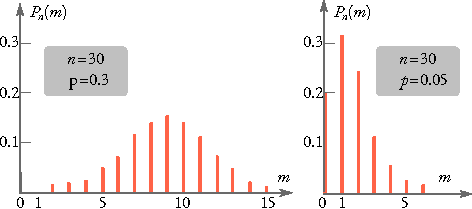
\includegraphics[width=0.9\tfwidth]{figures/poisson-gaussian.pdf}
\caption{The Poisson (right) and Gaussian (left) distributions.
\label{poisson-gaussian}}
 \end{figure}

\txthead{A Little of Mathematics.} The expression $(q + p)^{n}$, where $n$ is a positive integer, is called a binomial (two-term) expression of degree $n$. You should know about the binomial expansions of second and third degrees:
\begin{align*}
(q + p)^{2} & = q^{2}+ 2qp + p^{2}, \\
(q + p)^{3} & = q^{3} + 3q^{2}u + 3qp^{2} + p^{3}.
\end{align*}
In general (for a random integer $n$) the binomial expansion is
\begin{equation*}
(q+p)^{n} = q^{n} + nq^{n-1}p + \ldots + \frac{n(n-1) \ldots (n-m+1)}{m!} q^{n-m} p^{m} +
\ldots + nqp^{n-1} + p^{n}.
\end{equation*}
Using the notation given in (\ref{eq-1.8}), we can rewrite this formula as
\begin{equation*}
(q + p)^{n} = \mqty(n \\ 0) \, q^{n}
+  \mqty(n \\ 1)\, q^{n-1}p + \ldots
 +  \mqty(n \\ m) \, q^{n-m}p^{m} + \ldots
+  \mqty(n \\ n-1) \, qp^{n-1} +  \mqty(n \\ n) \, p^{n}.
\end{equation*}
Thus from (\ref{eq-1.9}), we can conclude that
\begin{equation*}
(q + p)^{n} = \sum_{m=0}^{n}  \mqty(n \\ m) \,  q^{n-m}p^{m} = \sum_{m=0}^{n}   P_{n}\,(m).
\end{equation*}
Consequently, the probabilities $P_{n}\, (m)$ coincide with the coefficients of
the binomial expansion, and this is why the \redem{binomial distribution} is so
called. The probabilities $q$ and $p$ in a binomial distribution are such that $q + p = 1$. Therefore, $(q + p)^{n} = 1$. On the other hand,
\begin{equation*}
(q+p)^{n} =  \sum_{m=0}^{n}   P_{n}\,(m).
\end{equation*}
Hence \eqref{eq-1.10}.

\section{Continuous Random Variables}

Continuous random variables are very unlike discrete ones.
A continuous variable can assume any of infinite set of values, which
continuously fill a certain interval. It is impossible in principle to list
every value or such a variable at the very least because there rs no such
thing as two neighbouring values (just as it is impossible to mark two
neighbouring points on the number axis). Besides, the probability of
a concrete value of a continuous random variable is zero.

\txthead{Can Probability Of A Possible Event Equal To Zero?} You know
now that an impossible event has a zero probability. However, a
possible event can also have a zero probability.

Suppose a thin needle is thrown many times at random onto a strip
of paper on which a number axis is marked. We can regard the
$x$-coordinate of the point where the needle crosses the number axis
(\figr{needle}~\drkgry{(a)}) to be a continuous random variable. This coordinate varies in a random fashion from one trial to another.

\begin{figure}[!h]
 \centering
 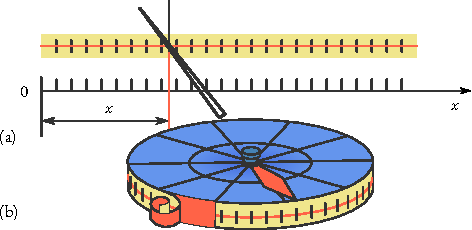
\includegraphics[width=0.8\tfwidth]{figures/needle.pdf}
\caption{The probability that a continuous random variable will take a
  certain value is zero.\label{needle}}
 \end{figure}
We could also use a roulette instead of throwing a needle. A strip of
paper with a numbered line could be. pasted to the circumference of
the roulette circle, as shown in \figr{needle}~\drkgry{(b)}. Wherever the freely
rotating arrow of the roulette is pointing when it stops, it yields a
number that will be a continuous random variable.

\begin{wrapfigure}{O}{\mfwidth}
 \centering
 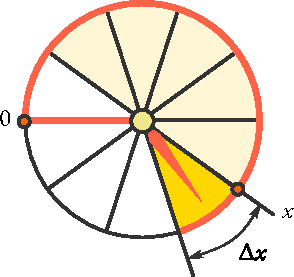
\includegraphics[width=0.9\linewidth]{figures/roulette.pdf}
\caption{A roulette to generate continuous random variables.\label{roulette}}
 \end{wrapfigure}

What is the probability of the arrow stopping at a certain point $x$?
In other words, what is the probability that a concrete value $x$ of a
continuous random variable is chosen? Suppose the roulette
circle's radius $R$ is divided into a finite number of identical
sectors, e.g. 10 sectors (\figr{roulette}). The length of the
arc corresponding to the sector equals $\Delta x = 2 \pi R/10$. The
probability that the arrow will stop within the sector hatched in the
figure is $\Delta x / 2 \pi R = 1/10$. Thus, the probability that the
random variable will take a value from $x$ to $x + \Delta x$ is
$\Delta x / 2 \pi R $. Let us gradually narrow the range of numbers,
i. e. divide the circle into larger numbers of sectors. The
probability $\Delta x / 2 \pi R $ that any value is in the range from
$x$ to $x + \Delta x$ also will fall. In order to obtain the
probability that the variable will take the value $x$ exactly, we must
find the limit as $\Delta x \to 0 $. In this case, the probability
$\Delta x / 2 \pi R $ becomes zero.  Thus we can see that the
probability that a continuous random variable will take a certain
value is indeed zero.

That event may be both possible and possess a zero probability may
seem paradoxical, but it is not. In fact there are parallels you are
surely well aware of. Consider a body of volume $V$ with a mass
$M$. Let us select a point $A$ within the body and consider a smaller
volume $V_{1}$ which contains the point (\figr{cubes}) and
assign a mass $M_{1}$ to it. Let us gradually shrink the smaller
volume around point $A$. We obtain a sequence of volumes containing
$A$, i.e. $V, V_{1}, V_{2}, V_{3}, \ldots ,$ and a corresponding
sequence of decreasing masses: $M, M_{1}, M_{2}, M_{3}, \ldots ,$. The
limit of the mass vanishes as the volume around $A$ contracts to
zero. We can see that a body which has a finite mass consists of
points which have zero masses. In other words, the nonzero mass of the
body is the \redem{sum of an infinite number of zero masses} of its
separate points. In the same way, the nonzero probability that a
roulette arrow stops within a given range $\Delta x$ is the \redem{sum
  of an infinite number of zero probabilities} that the arrow will
stop at each individual value within the considered range.

\begin{wrapfigure}{O}{\mfwidth}
 \centering
 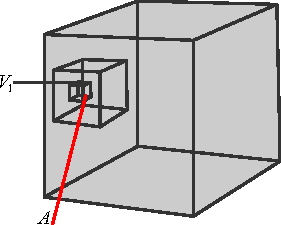
\includegraphics[width=0.9\linewidth]{figures/cubes.pdf}
\caption{A finite non-zero mass can be generated from the sum of an infinite number of zero masses.\label{cubes}}
 \end{wrapfigure}

\txthead{The Density Of A Probability.} This conceptual difficulty can
be avoided by using the idea \redem{density}. Although the mass of a
point within a body is zero, the body's density at the point is
non-zero. If $\Delta M$ is the mass of a volume $\Delta V$ within which
the point in question is located (we shall describe the point in terms
of its position vector $\vb{r}$, then the density $\rho \, (\vb{r})$ at
this point is the limit of the ratio $ \Delta M/ \Delta V$ as $\Delta V$ converges to the
point at $\vb{r}$, i.e.,
\begin{equation*}%
\rho \, (\vb{r}) = \lim_{\Delta V \to 0}  \frac{\Delta M}{\Delta V}.
\end{equation*}
If the volume $\Delta V$ is small enough, we can say that $\Delta M
\simeq \rho (\vb{r}) \Delta V$. Using a strict approach, we should
substitute $\Delta V$ by the differential $\dd V$.

The mass $M$ of a body occupying volume $V$ is then expressed by the
\redem{integral}:
\begin{equation*}%
  M = \int_{V} \rho \,  (\vb{r}) \, \dd V,
\end{equation*}
over the volume in question.


Probability theory uses a similar approach. When dealing with
\redem{continuous} random variables, the \redem{probability density} is used rather than the probability itself. Let $f(x)$ be the probability density of a random variable $x$, and so by analogy with the mass density we have
\begin{equation*}%
f(x) = \lim_{\Delta x \to 0 }   \frac{\Delta p_{x}}{\Delta x}.
\end{equation*}
Here $\Delta p_{x}$ is the probability that a random variable will take a value
between $x$ and $x + \Delta x$. The probability $p$ that a random variable will
have a value between $x_{1}$ and $x_{2}$ is, in terms of probability density, as
follows:
\begin{equation}%
p = \int\limits_{x_{1}}^{x_{2}} f(x) \dd x.
\label{eq-1.15}
\end{equation}
If the integration is over the whole range of values a random variable
may take, the integral (\ref{eq-1.15}) will evaluate to unity (this is the probability of a certain event). In the example with a roulette mentioned above,
the whole interval is from $x = 0$ to $x = 2 \pi R$. In general, we assume the
interval is infinite, when 
\begin{equation}%
 \int\limits_{- \infty}^{+ \infty} f(x) dx = 1.
\label{eq-1.16}
\end{equation}
The integral is very simple in the roulette example because the
probability the roulette arrow stops within an interval from $x$ to $x
+ \Delta x$ \redem{does not depend on} $x$. Therefore, the probability
density does not depend on $x$, and hence,


A similar situation is encountered when the density of a body is the
same at every point, i.e. when the body is \redem{uniform} $(\rho = M/V)$. More
generally, density $\rho (\vb{r})$ varies from point to point, and so does the
probability density $f (x)$.


\txthead{The Expected Value And The Variance Of A Continuous Random Variable.} The \redem{expected value} and \redem{variance} of a discrete random
variable are expressed as sums over the probability distribution (see
equations \eqref{eq-1.4} to \eqref{eq-1.6}. When the random variable is
continuous, integrals are used instead of sums and the probability
density distribution is used rather than the probability distribution:
\begin{align}%
E(x) & =  \int\limits_{- \infty}^{+ \infty} x f(x) \, \dd x, 
\label{eq-1.17}\\
\text{var} & =  \int\limits_{- \infty}^{+ \infty} (x - E(x))^{2} f(x) \, \dd x.
\label{eq-1.18}
\end{align}

\txthead{The Normal Distribution Of Probability Density.}
The normal distribution of probability density. When dealing with
continuous random variables, we often encounter the \redem{normal}
distribution of probability density. This distribution is defined by the
following expression (compare it with \eqref{eq-1.13}):
\begin{equation}
f(x) = \frac{1}{\sigma \sqrt{2 \pi}} \exp \left( - \frac{(x - E(x))^2}{2 \sigma ^{2}}\right).
\label{eq-1.19}
\end{equation}

Here $\sigma$ is the standard deviation ($\sigma = \sqrt{var}$) the
function \eqref{eq-1.19} is called the \redem{normal} or \redem{Gaussian
  distribution}.

The probability density of a continuous random variable is always
normal if the variance of its values is due to many different equally
strong factors. It has been proved in probability theory that the sum of
a large enough number of independent random variables obeying any
distributions tends to the normal distribution, and the larger the number
of sums the more accurately the normal distribution is.



For instance, suppose we are dealing with the production of nuts and
bolts. The scatter of the inside diameter of the nut is due to random
deviations in the properties of the metal, the temperature, vibration of
the machine tool, changes in the voltage, wear of the cutter, etc. All of
these effects act independently and approximately with the same
strength. They are superimposed, and the result is that the inside
diameter of the nuts is a continuous random variable with a normal
distribution. The expected value of this variable should evidently be the
desired inside diameter of the nuts, while the variance characterizes the
scatter of the obtained diameters around the desired value.


\begin{figure}[!ht]
 \centering
 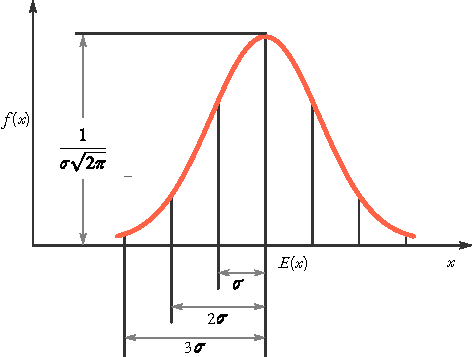
\includegraphics[width=0.75\tfwidth]{figures/three-sigma.pdf}
\caption{The three-sigma rule for a Gaussian distribution.\label{three-sigma}}
 \end{figure}



\txthead{The Three-Sigma Rule.}  A normal distribution is shown in
\figr{three-sigma}. It has a maximum at the expected value $E
(x)$. The curve (the \redem{Gaussian curve}) is bell-shaped and is
symmetric about $E (x)$. The area under the entire curve, i. e. for
the interval $(- \infty < x < + \infty )$, is given by the integral
$ \int_{- \infty}^{+ \infty} f(x) dx$.  Substituting \eqref{eq-1.19}
here, it can be shown that the area is equal to unity. This agrees
with \eqref{eq-1.16}, whose meaning is that the probability of a certain event
is unity. Let us divide the area under the Gaussian curve using
vertical lines (see \figr{three-sigma}). Let us first consider the section
corresponding to the interval  $E (x) -  \sigma  \leq x \leq E(x) + \sigma $. It can be shown (please believe me) that 
\begin{equation*}
\int\limits_{E(x) - \sigma}^{E(x) + \sigma} f(x) dx = 0.683. 
\end{equation*}
This means that the probability of $x$ taking a value in the interval from $E
(x) - \sigma$ to $E (x) + \sigma $ equals 0.683. It can also be calculated that
the probability of $x$ taking a value from $E (x) - 2 \sigma$ to $E
(x) + 2 \sigma $ is 0.954, and the probability of $x$ taking a value in the range of $E (x) - 3 \sigma $ to $E (x) + 3 \sigma $ is 0.997. Consequently, a continuous random variable with a normal distribution takes a value in the interval $E (x) - 3 \sigma $ to $ E(x) + 3 \sigma $ with probability 0.997. This probability is practically equal to unity. Therefore, it is natural to assume for
all practical purposes that a random variable will always take a value in the interval from $3 \sigma$ on the right to $3 \sigma$ on the left of $E (x)$. This is called the \redem{three-sigma rule}.
%%% Local Variables:
%%% mode: latex
%%% TeX-engine: xetex
%%% TeX-master: "twibop2"
%%% End:

% !TEX root = twibop2.tex
\chapter{Decision Making}
\epigraph{Practical demands brought forth special scientific methods
  that can be collected under the heading ``operations research''. We
  shall use this term to mean the application of quantitative
  mathematical methods to justify decisions in every area of
  goal-oriented human activity.}  {E. S. Wentzel}

\section{These Difficult Decisions}

\txthead{Decision making under uncertain conditions.} We often have to make decisions when not all the information is
available and this uncertainty always decreases to some extent our
ability to decide. For example, where to go for a vacation or holiday?
This has worried me many times, since various uncertainties concerning
the weather, the hotel, the entertainment at the resort, and so on,
must be foreseen. We try and decide on the best variant from our
experience and the advice of our friends, and we often act ``by
inspiration''. This \redem{subjective} approach to decision making is
justifiable when the consequences involve ourselves and
relatives. However, there are many situations when a decision can
affect a large number of people and therefore requires a \redem{scientific}
and \redem{mathematically justifiable} approach rather than a
subjective one.


For instance, modern society cannot function without electricity,
stores of food, raw materials, etc. The stores are kept everywhere: at
factories, shops, hospitals, and garages. But how large should the
stores be in a particular case? It is clear that they should not be
too small, otherwise the function of the enterprise would be
interrupted. Neither should they also be too large because they cost
money to build and maintain: they would be dead stock. \redem{Store-keeping} is a problem of exceptional importance. It is so complicated because a decision must always be made in conditions of uncertainty.

\txthead{Two kinds of uncertainty.} How should we make decisions under conditions of uncertainty? First of
all, we should discover which factors are causing the uncertainty and
evaluate their nature. There are two kinds of uncertainty. The first
kind is due to factors which can be treated using the theory of
probability. These are either \redem{random variables} or \redem{random
  functions}, and they have statistical properties (for instance, the
expected value and variance), which are either known or can be
obtained over time. Uncertainty of this kind is called
\redem{probabilistic} or \redem{stochastic}. The second kind of
uncertainty is caused by unknown factors which are not random
variables (random functions) because the set of realizations of these
factors does not possess statistical stability and therefore the
notion of probability cannot be used. We shall call this uncertainty
``bad''.

``So'', the reader may say, ``it would seem that not every event that
cannot be predicted accurately is a random event.''

``Well, yes, in a way.'' Let me explain. In the preceding chapter we
discussed random events, random variables, and random functions.  I
repeatedly emphasized that there should always be \redem{statistical
  stability}, which is expressed in terms of probability. However,
there are events, which occur from time to time, that do not have any
statistical stability. The notion of probability is inapplicable to
such events, and therefore, the term ``random'' cannot be used here
too. For instance, we cannot assign a probability to the event of an
individual pupil getting an unsatisfactory mark in a concrete
subject. We cannot, even hypothetically, devise a set of uniform
trials that might yield the event as one outcome. There would be no
sense in conducting such a trial with a group of pupils because each
pupil has his or her own individual abilities and level of preparation
for the exam. The trials cannot be repeated with the same pupil
because he will obviously get better and better in the subject from
trial to trial. Similarly there is no way we can discuss the
probability of the outcome of a game between two equally matched chess
players. In all such situations, there can be no set of uniform
trials, and so there is no stability which can be expressed in terms
of a probability. We have ``bad'' uncertainty in all such situations.


I am afraid we do not consider the notion ``statistical stability'' and
often use expressions such as ``improbable'', ``probable'', ``most
probable'', and ``in all probability'' to refer to events that cannot be
assigned by any probability. We are apt to ascribe a probability to every
event even though it might not be predictable. This is why it became
necessary to refine the notion of probability early this century. This was
done by A.N. Kolmogorov when he developed an axiomatic definition
of probability.

\txthead{Options and the measure of effectiveness.} When we speak of
decision making, we assume that different patterns of behaviour are
possible.  They are called \redem{options}. Let me emphasize that in
the more important problems the number of options is very great. Let
$X$ be the set of options in a particular situation. A decision is
made when we select one option $x$ from this set. How do we determine
which option is the most preferable or the most efficient? A
quantitative criterion is needed to allow us to compare different
options in terms of their effectiveness. Let us call this criterion
the \redem{measure of effectiveness}. This measure is selected for each
particular \redem{purpose}, e.g., not to be late for school, to solve a
problem correctly and quickly, or to reach the cinema. A doctor wants
to find an efficient method of treating his patient. A factory manager
is responsible for the fulfilment of a production plan. The most
efficient option is the one that suits its purpose best.


Suppose we work in a shop and our target is to maximize the
receipts. We could choose profit as the measure of effectiveness and
strive to maximize this measure. The selection of the measure in this
example is evident. However, there are more complicated situations,
when several goals are pursued simultaneously, for example, we wish to
maximize profit, minimize the duration of the sales, and distribute the
goods to the greatest number of customers. In such cases we have to
have several measures of effectiveness; these problems are called
multi-criterial.

Let $W$ be a single measure of effectiveness. It would seem that our
task is now to find an option $x$ at which $W$ is at a maximum (or, the
other way round, at a minimum). However, we should remember that
decision making occurs under conditions of uncertainty. There are
unknown (random) factors (let us use $\xi$ to denote them), which influence
the end result and therefore affect the measure of effectiveness $W$. There
is also always a set of factors known beforehand (let us designate them
$\alpha$). Therefore the measure of effectiveness is dependent on three groups
of factors: known factors $\alpha$, unknown (random) factors $\xi$, and the
selected option $x$:
\begin{equation*}%
W= W(\alpha, \xi, x).
\end{equation*}
In the sales example, the $\alpha$ set is goods on sale, the available premises,
the season, etc. The $\xi$ factors include the number of customers per day
(it varies randomly from day to day), the time customers arrive (random
crowding is possible, which leads to long queues), the goods chosen by
the customers (the demand for a given commodity varies randomly in
time), etc.

Since the $\xi$, factors are random, the measure of effectiveness $W$ is
a random variable. Now, how is it possible to maximize (minimize)
a random variable? The answer quite clearly is that it is naturally
impossible. Whichever option $x$ is chosen, $W$ remains random, and it
cannot be maximized or minimized. This answer should not discourage
the reader. It is true that under conditions of uncertainty we cannot
maximize (minimize) the measure of effectiveness with a hundred per
cent probability. However, an adequate selection of an option is possible
with a reasonably large probability. This is where we should tackle the
techniques used in decision making under conditions of stochastic
uncertainty.

\txthead{Substitution of random factors by means.} The easiest
technique is merely to substitute the random factors $\xi$ by their
means. The result is that the problem becomes completely determined
and the measure of effectiveness $W$ can be calculated precisely. It
can, in particular, be either maximized or minimized. This technique
has been widely used to solve problems in physics and
technology. Almost every parameter encountered in these fields (e.g.,
temperature, potential difference, illuminance, pressure) is, strictly
speaking, a random variable. As a rule, we neglect the random nature
of physical parameters and use their mean values to solve the
problems.

The technique is justified if the deviation of a parameter from its
mean value is insignificant. However, it is not valid if the random factor
significantly affects the outcome. For instance, when organizing the jobs
in a motor-car repair shop, we may not neglect the randomness in the
way cars fail, or the random nature of the failures themselves, or the
random time needed to complete each repair operation. If we are
dealing with the noise arising in an electronic device, we cannot neglect
the random behaviour of electron flows. In these examples, the $\xi$ factors
must indeed be considered as random factors, we shall say they are
essentially random.

\txthead{Mean value optimization.} If the $\xi$ factors are essentially
random, we can use a technique called \redem{mean-value
  optimization}. What we do is to use the expected value $E (W)$ as the
measure of effectiveness, rather than the random variable $W$ and the
expected value is maximized or minimized.

Naturally, this approach does not resolve the uncertainty. The
effectiveness of an option $x$ for concrete values of random
parameters $\xi$ may be very different from the expected one. However,
using mean-value optimization means that we can be sure that after
many repeated operations we shall gain overall. It should be borne in
mind that mean-value optimization is only admissible when the gains of
repeated operations are \redem{totalled}, so that ``minuses'' in some
operations are compensated by the ``pluses'' in others. Mean-value
optimization would be justified should we be trying to increase the
profit obtained, for instance, in a sales department. The profit on
different days would be totalled, so that random ``unlucky'' days
would be compensated by the ``lucky'' days,

But here is another example. Suppose we consider the effectiveness of
the ambulance service in a large city. Let us select the elapsed time
between summoning help and the ambulance arriving as the measure of
effectiveness. It is desirable that this parameter be minimized. We cannot
apply mean-value optimization because if one patient waits too long for
a doctor, he or she is not compensated by the fact that another patient
received faster attention.

\txthead{Stochastic constraints.} Let us put forward an additional
demand.  Suppose we desire that the elapsed time $W$ till the arrival
of help after a call for an ambulance be less than some value
$W_{0}$. Since $W$ is a random variable, we cannot demand that the
inequality $W< W_{0}$ be always true, we can only demand that it be
true for some large probability, for instance, no less than 0.99. In
order to take this into account we delete from the $X$ set those
options $x$, for which the requirement is not satisfied. These
\redem{constraints} are called \redem{stochastic}.  Naturally, the use
of stochastic constraints noticeably complicates decision making.


\section{Random Processes with Discrete States}
A \redem{random} process can be thought of as the transition of a system from
one state to another occurring in a random fashion. We shall consider
random processes with \redem{discrete states} in this chapter and so our system
will be supposed to have a set of discrete states, either finite or infinite.
The random transitions of the system from one state to another are
assumed to take place \redem{instantaneously}.

\txthead{State graphs.} Random processes with discrete states can be
conveniently considered using a diagram called a \redem{state graph}. The
diagram shows the possible states a system may be in and indicates the
possible transitions using arrows.
 \begin{wrapfigure}[12]{O}{\mfwidth}
 \centering
 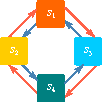
\includegraphics[width=0.9\linewidth]{figures/state-graph1.pdf}
\caption{A state graph for system with four states.}
\label{state-graph1}
 \end{wrapfigure}
 
Let us take an example. Suppose a system consists of two machine
tools, each of which produces identical products. If a tool fails its repair
is started immediately. Thus, our system has four states: $S_{1}$ both tools
are operating; $S_{2}$ the first tool is under repair after a failure while the
second is operating; $S_{3}$, the second tool is under repair while the first is
operating; $S_{4}$, both tools are being repaired.

The state graph is given in \figr{state-graph1}. The transitions
$S_{1} \to S_{2}, \,\, S_{1} \to S_{3}, \,\, S_{2} \to S_{4}$ and
$S_{3} \to S_{4}$ occur as a result of failures in the system. The
reverse transitions take place upon termination of the
repairs. Failures occur at unpredictable moments and the moments when
the repairs are terminated are also random. Therefore, the system's
transition from state to state is random.



 Note that the figure does not show transitions $S_{1} \to S_{4}$ and
 $S_{4} \to S_{1}$.  The former corresponds to the simultaneous
 failure of both tools and the latter to the simultaneous termination
 of repair of both tools. We shall assume that the probabilities of
 these events are zero.

 \txthead{Event arrival.} Suppose that we have a situation in which a
 \redem{stream of uniform events} follow each other at random moments. They
 may be telephoned orders for taxi, domestic appliances being switched
 on, the failures in the operation of a device, etc.

 \begin{figure}[!ht]
 \centering
 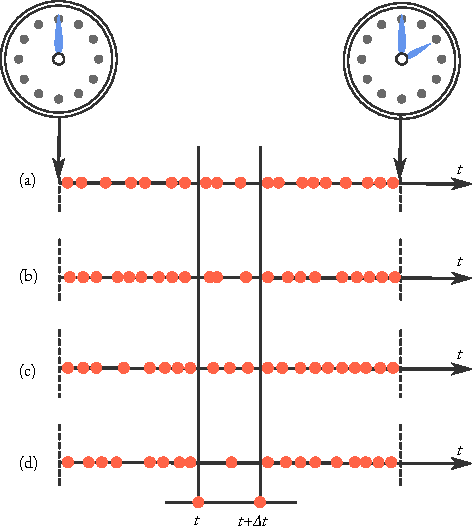
\includegraphics[width=0.85\tfwidth]{figures/event-arrival.pdf}
\caption{A record of taxi orders at a taxi depot.\label{event-arrival}}
 \end{figure}


 Suppose the dispatcher at a taxi depot records the time each taxi
 order is made over an interval of time, for instance, from 12 a.m. to
 2 p.m. We can show these moments as points on the time axis, and so
 the dispatcher might get the pattern illustrated in 
 \figr{event-arrival}~\drkgry{(a)}. This is the realization of the taxi-call arrivals  during that interval of time. Three more such realizations are shown
 in \figr{event-arrival}~\drkgry{(b)}, \drkgry{(c)}, and \drkgry{(d)}, and they are patterns recorded on different days. The moments when each taxi order is made
 in each realization are random. At the same time, the taxi-order arrivals possess statistical stability, that is, the total number of events in each interval of time varies only slightly from experiment to experiment
(from one arrival realization to another). We can see that the number of
events in the arrival realisations presented are 19, 20, 21, and 18.

In the preceding chapter, a random event in an experiment was an
outcome which has a definite probability. When we are considering
arrivals of events, we must have another meaning for the term
``event''.  There is no use speaking about the probability of an
outcome (event) because each event is uniform, i.e. indistinguishable
from the others. For instance, one taxi-order is a single event in a
stream and is indistinguishable from another event. Now let us
consider other probabilities, for instance, the probabilities that an
event will occur during a given interval of time (suppose, from $t$ to
$t + \Delta t$, as shown in the figure) exactly once, twice, thrice,
etc.

The notion of ``event arrival'' is applied to random processes in
systems with discrete states. It is assumed that the transitions of a
system from one state to another occur as a result of the effect of
event arrivals. Once an event arrives, the system instantaneously
changes state. For the state graph in \figr{state-graph1} transitions
$S_{1} \to S_{2}$ and $S_{3} \to S_{4}$ occur due to the arrival of
events corresponding to failures in the first tool, while transitions
$S_{1} \to S_{3}$ and $S_{2} \to S_{4}$ occur due to failures of the
second tool. The reverse transitions are caused by the arrival of
events corresponding to the ``terminations'' of repair: transitions
$S_{2} \to S_{1}$ and $S_{4} \to S_{3}$, are caused by the arrivals of
repair terminations of the first tool, and transitions
$S_{3} \to S_{1}$ and $S_{4} \to S_{2}$ to the arrivals of repair
terminations of the second tool.

The system transfers from state $S_{i}$ to state $S_{j}$ every time
the next event related to the transition arrives. The natural
conclusion is that the probability of transition $S_{i} \to S_{j}$ at
a definite moment in time $t$ should equal the probability of an event
arrival at this moment. There is no sense in speaking of the
probability of a transition at a concrete moment $t$. Like the
probability of any concrete value of a continuous random variable,
this probability is zero, and this result follows from the continuity
of time. It is therefore natural to discuss the probability of a
transition (the probability of an event arrival) occurring during the
interval of time from $t$ to $t+ \Delta t$, rather than its occurrence
at time $t$. Let us designate this probability $P_{ij}(t, \Delta
t)$. As $\Delta t$ tends to zero, we arrive at the notion of a
\redem{transition probability density} at time $t$, i.e. 
\begin{equation}%
\lambda_{j} (t) = \lim_{\Delta t \rightarrow 0} x =  \frac{P_{ij}\,(
  t, \Delta t)}{\Delta t}.
\label{eq-2.1}
\end{equation}
This is also called the \redem{arrival rate of events} causing the transition in
question.

In the general case, the arrival rate depends on time. However, it should
be remembered that the dependence of the arrival rate on time is
not related to the location of ``dense'' or ``rare'' arrival realisations. For
simplicity's sake, we shall assume that the transition probability density
and therefore the event arrival rate does not depend on time. i.e. we
shall consider \redem{steady-state} arrivals.


 \begin{wrapfigure}{O}{\mfwidth}%[h]
 \centering
 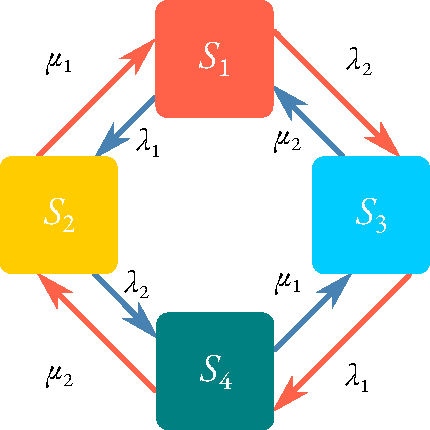
\includegraphics[width=0.9\linewidth]{figures/state-graph2.pdf}
\caption{A state graph for system with four states with arrival rates.
\label{state-graph2}}
 \end{wrapfigure}
 
\txthead{The Chapman-Kolmogorov equations for steady state.} Let us
use $p_{i}$ to denote the probability that a system is in state
$S_{i}$ (since our discussion is only for \redem{steady-state}
arrivals, the probabilities $p_{i}$, are independent of time), Let us
consider the system whose state graph is given in \figr{state-graph1}. Suppose $\lambda_{1}$ is the arrival rate for failures of the first tool and $\lambda_{2}$ that for the second tool; let $\mu_{1}$ be the arrival rate for repair terminations of the first tool and $\mu_{2}$ that for the second tool. We have labelled the state graph with the appropriate arrival rates, see \figr{state-graph2}.



 Suppose there are $N$ identical systems described by the state graph
 in \figr{state-graph2}. Let $N \gg 1$. The number of systems with
 state $S_{i}$, is $N p_{i}$ (this statement becomes more accurate the
 larger $N$ is). Let us consider a concrete state, say,
 $S_{1}$. Transitions are possible from this state to states $S_{2}$
and $S_{3}$ with probability $\lambda_{1} + \lambda_{2}$, per unit
time. (Under steady state, the probability density is the probability
for the finite time interval $\Delta t$ divided by $\Delta t$.)
Therefore, the number of departure: from state $S_{1}$, per unit time in
the considered set of systems is $N p_{ 1}\, (\lambda_{1}+\lambda_{2})$,
We can discern a general rule here: the number of transitions
$S_{i} \to S_{j}$ per unit time is the product of the number of
systems with state $S_{i}$ (the initial state) by the probability of
the transition per unit time, We have considered departures from state
$S_{1}$. The system arrives at this state from $S_{2}$ and $S_{3}$, The number
of arrivals at $S_{1}$ per unit time is $N p_{2} \, \mu_{1} + N p_{3}
\, \mu_{1}$. Since we are dealing
with steady states, the number of departures and arrivals for each
particular state should be balanced.  Therefore.  
\begin{equation*}%
N p_{ 1}(\lambda_{1}+\lambda_{2}) = N p_{2} \, \mu_{1} + N p_{3} \, \mu_{2}.
\end{equation*}
By setting up similar balances of arrivals and departures for each of
the four states and eliminating the common factor $N$ in the equations, we obtain the following equations for probabilities $p_{1}, \, p_{2},
\, p_{3}$ and $p_{4}$:
\begin{align*}%
\text{for state} \,\,  S_{1}: (\lambda_{1} + \lambda_{2}) \, p_{1} &
= \mu_{1} p_{2} + \mu_{2} p_{3}, \\
\text{for state} \,\,  S_{2}: (\lambda_{2} + \mu_{1}) \, p_{2} &
= \lambda_{1} p_{1} + \mu_{2} p_{4}, \\
\text{for state} \,\,  S_{3}: (\lambda_{1} + \mu_{2}) \, p_{3} &
= \lambda_{1} p_{1} + \mu_{1} p_{4}, \\
\text{for state} \,\,  S_{4}: (\mu_{1} + \mu_{2}) \, p_{4} &
= \lambda_{2} p_{2} + \lambda_{1} p_{3}. 
\end{align*}
It is easy to see that the fourth equation can be obtained by summing
the first three. Instead of this equation, let us use the equation
\begin{equation*}%
p_{1}+p_{2}+p_{3}+p_{4}= 1,
\end{equation*}
which means that the system must be in one of the four states.
Therefore, we have the following system of equations:
\begin{equation}%
\left.
\begin{split}
S_{1}: (\lambda_{1} + \lambda_{2}) \, p_{1} & = \mu_{1} p_{2} + \mu_{2} p_{3}, \\
S_{2}: (\lambda_{2} + \mu_{1}) \, p_{2} & = \lambda_{1} p_{1} + \mu_{2} p_{4}, \\
S_{3}: (\lambda_{1} + \mu_{2}) \, p_{3} & = \lambda_{2} p_{1} + \mu_{1} p_{4},  \\
p_{1} + p_{2} + p_{3} + p_{4} & = 1.
\end{split}
\right\}
\label{eq-2.2}
\end{equation}
These are the \redem{Chapman-Kolmogomv equations} for the system whose state
graph is shown in \figr{state-graph2}.

\txthead{Which innovation should be chosen?} Let us analyze a concrete
situation using equations \eqref{eq-2.2}. The state graph (see \figr{state-graph2})
corresponding to these equations describes a system which, we assumed,
consists of two machine tools each producing identical goods Suppose
the second tool is more modern an its output rate is twice that o the
first tool. The first tool generates (per unit time) an income of five
conventional units, while the second one generates one of ten units.
Regretfully, the second tool fails, on the average, twice as
frequently as does the first tool: hence $\lambda_{1} = 1$ and
$\lambda_{2} =2$. The arrival
rates for repair termination are assumed to be $u_{1} =2$ and $u_{2} =3$. Using
these arrival rates for failure and repair termination. let us rewrite
(\ref{eq-2.2}) thus 
\begin{equation*}
\left.
\begin{split}
3p_{1} & = 2p_{2} + 3p_{3}, \\
4p_{2} & = p_{1} + 3p_{4}, \\
4p_{3} & = 2p_{1} + 2p_{4}, \\
p_{1} +p_{2}&+p_{3}+p_{4}= 1.
\end{split}
\right\}
\end{equation*}
This system of equations can be solved to yield
$p_{1}= 0.4, \, p_{2}=0.2, \, p_{3} = 0.27$ and $p_{4} = 0.13$. This
means that, on the average, both tools operate simultaneously (state
$S_{1}$ in the figure) 40 per cent of the time, the first tool operates
while the second one is being repaired (state $S_{2}$) 20 per cent of
the time, the second tool operates while the first one is being
repaired (state $S_{3}$) 27 per cent of the time, and both tools are
simultaneously being repaired (state $S_{4}$) 13 per cent of the
time. It is easy to calculate the income this tool system generates
per unit time: $(5+10) \times 0.4+5 \times 0.2+10 \times 0.27 =9.7$
conventional units.

Suppose an innovation is suggested which would reduce the repair time of either the first or second tool by a factor of two. For technical reasons, we can only apply the innovation to one tool. Which tool should be chosen, the first or the second? Here is a concrete example of a practical situation when, using probability theory, we must justify our decision scientifically

Suppose we choose the first tool. Following the introduction of the
innovation, the arrival rate of its repair termination increases by a
factor of two, whence $u_{1} = 4$ (the other rates remain the same,
i. e. $\lambda_{1} = 1, \lambda_{2} = 2$ and $\mu_{2} =3$). Now
equations \eqref{eq-2.2} are 
\begin{equation*}
\left.
\begin{split}
3p_{1} & = 4p_{2} + 3p_{3}, \\
6p_{2} & = p_{1} + 3p_{4}, \\
4p_{3} & = 2p_{1} + 4p_{4}, \\
p_{1} +p_{2}&+p_{3}+p_{4}= 1.
\end{split}
\right\}
\end{equation*}
After solving this system, we find that $p_{1} = 0.48, p_{2} = 0.12, p_{3} = 0.32$, and $p_{4} =0.08$. These probabilities can be used to calculate the income our system will now generate: $(5+ 10) \times 0.48+5 \times 0.12+ 10 \times 0.32 = 11$ conventional units. 

If we apply the innovation to the second tool, the rate $\mu_{2}$, will be doubled. Now $\lambda_{1}  = 1,\, \lambda_{2} = 2, \, \mu_{1} = 2$ and $\mu_{2} = 6$, and equations (\ref{eq-2.2}) will be 
\begin{equation*}
\left.
\begin{split}
3p_{1} & = 2p_{2} + 6p_{3}, \\
4p_{2} & = p_{1} + 6p_{4}, \\
7p_{3} & = 2p_{1} + 2p_{4}, \\
p_{1} +p_{2}&+p_{3}+p_{4}= 1.
\end{split}
\right\}
\end{equation*}
This system yields: $p_{1} = 0.5, p_{2} = 0.25, p_{3} = 0.17$, and $p_{4} =0.08$,
whence the Income is $(5+ 10) \times 0.5+5 \times 0.25+10 \times 0.17=10.45$
conventional units. Therefore it is clearly more profitable to apply
the innovation to the first too.

\section{Queueing Systems}

\txthead{The problem of queueing.} Modern society cannot exist without
a whole network of \redem{queueing systems}. These include telephone
exchanges, shops, polyclinics, restaurants, booking offices, petrol
stations, and hairdressers.  Despite their diversity, these systems
have several things in common and common problems.

When we seek the assistance of a doctor or service from a cafe,
restaurant, or barber, we must wait for our turn in a queue, even if we
telephone to make an appointment, that is, reserve our place in a queue
without actually attending physically. Clearly, we wish to be served
straight away and waiting can be frustrating.

It is clear that the source of the problem is the \redem{random nature} of the
demands for attention in queueing systems. The arrival of calls at
a telephone exchange is random as is the duration of each telephone
conversation. This randomness cannot be avoided. However, it can be
taken into account and, as a consequence, we can rationally organize
a queueing system for all practical purposes. These problems were first
investigated in the first quarter of this century. The mathematical
problems for simulating random processes in systems with discrete states
were formulated and considered, and a new field of investigation in
probability theory was started.

Historically, queueing theory originated in research on the
overloading of telephone exchanges, a severe problem in the early 20th
century. The initial period in the development of the queueing theory
can be dated as corresponding to the work of the Danish scientist
A. Erlang in 1908-1922. Interest in the problems of queueing rapidly
increased. The desire for more rational servicing of large numbers of
people led to investigations of queue formation. It soon became
evident that the problems dealt with in queueing theory went well
beyond the sphere of rendering service and the results are applicable
to a wider range of problems.

Suppose a workman is operating several machine tools. Failures
requiring urgent repairs occur at random moments, and the duration of
each repair is a random variable. The result is a situation similar to
a common queueing system. However, this is a problem of servicing
many tools by a worker rather than servicing many people by
a queueing system.

The range of practical problems to which queueing theory can be
applied is uncommonly wide. We need the theory when we want, say, to
organize the efficient operation of a modern sea port, when, for instance,
we analyze the servicing rate of a large berth. We apply to queueing
theory when we look at the operation of a Geiger-M\"uller counter. These
devices are used in nuclear physics to detect and count ionizing
particles. Each particle entering a tube in the counter ionizes gas in the
tube, the ionization being roughly independent of the particle‘s nature
and energy, and so a uniform discharge across the tube is generated. But
when one discharge is under way, a new particle cannot be registered
(``serviced'') by the same counter. The moment each particle enters the
tube 5 random, as is the duration of the discharge (the ``servicing'' time).
This is a situation typical for queueing systems.

\txthead{Basic notions.} A queueing system is set up to organize the service of
a \redem{stream of requests}. The request may be a new passenger in a booking
office, a failure in a machine tool, a ship mooring, or a particle entering
a Geiger-M\"uller counter. The system may have either one or several
\redem{servers}. When you go to a large barbershop or hairdresser and want to
know the number of barbers or hairdressers, you are in effect asking for
the number of servers in the establishment. In other situations, the
servers may be the number of cashiers in a booking office, the number
of telephones at a post office for making trunk calls, the number of
berths in a port, or the number of pumps at a petrol station. If, on the
other hand, we wish to see a particular doctor, we are dealing with
a single-server queueing system.

When we consider the operation of a queueing system, we must first
take into account the number of servers, the number of requests arriving
at the system per unit time, and the time needed to service a request.
The number of requests arriving at the system, the moments they arrive,
and the time needed to service a request are, as a rule, \redem{random} factors.
Therefore, queueing theory is a \redem{theory of random processes}.

Random processes of this type (i. e. with \redem{discrete states}) were discussed
in the preceding section. A system transfers from state to state when each request arrives at the system and when the requests are serviced. The latter is given by the rate at which requests can be served by a single, continuously occupied server.

\txthead{Queueing systems.} There are two sorts of queueing system: \redem{systems with losses} and \redem{systems with queues}. If a request arrives at a system with losses when all the servers are occupied, the request is ``refused'' and is then lost to the system. For example, if we want to telephone someone
and the number is engaged, then our request is refused and we put
down the receiver. When we dial the number again, we are submitting
a new request.

The more common types of system are those with queues or systems
with waiting. This is why it is called the \redem{theory of queueing}. In such
a system, if a request (or customer) arrives when all the servers are
occupied, the customer takes a place in a \redem{queue} and waits for a server to become free. There are systems with \redem{infinite queues} (a queueing customer is eventually served and the number of places in the queue is unlimited) and systems with \redem{finite queues}. There are different sorts of restriction, i.e. the number of customers queueing at the same time may be limited (the queue cannot be longer than a certain number of customers and any new customer is refused); the duration of a customer's stay in the queue
may be limited (after a certain length of time queueing, an unserved
customer will leave the queue); or the time the system operates for may
be restricted (customers may only be served for a certain interval of
time).

The service order is also important. Customers are commonly served
``first come first served''. However, \redem{priority servicing} is also
possible, i.e. a newcomer to a queue is served first irrespective of
the queue.  A customer with a high priority may arrive at the system
and interrupt the servicing of a customer with a lower priority, which
may already start, or the higher priority customer may have to wait
until the servicing has been completed. The priority is \redem{absolute} in
the first case and \redem{relative} in the second. Queueing systems are always
\redem{multi-critical}, that is, they have a \redem{set} of measures by which their effectiveness can be estimated. These may be the average number of
customers served by the system per unit time, the average number of
occupied servers, the average number of customers in the queue, the
average time of waiting for servicing, the average percentage of
refused customers, and the probability a customer arriving at the
system is immediately served. There are other measures of such
systems' effectiveness. It is quite natural that when organizing the
operation of a queueing system we should strive to reduce the average
number of customers in the queue, and to reduce the time of waiting
for servicing. It is also desirable to maximize the probability that a
customer arriving at the s stem is served immediately, to minimize the
average percentage of refused customers, and so on. 

This eventually means that the productivity of the system must be increased (i.e. the time needed to service each customer be decreased), the system's
operation be rationalized, and the number of servers made as large as
possible. However, by raising the number of servers, we cannot avoid
decreasing the average number of occupied servers. This means that the
duration of the time for which a server is not occupied will increase,
i.e. the server will be idle for some time. The result is that the
system's operational efficiency is lowered. Therefore we must in some
way \redem{optimize} the system's operation. The number of servers should not
be too small (to eliminate long queues and to keep the number of
refusals small), but it should also not be too large (so that the
number and duration of idle periods for each server is small).

\txthead{Systems with losses.} The simplest type of queueing system is
a \redem{single-server system with losses}. Here are some examples: a system with only one telephone line or a particle detector consisting of only one
Geiger-M\"uller counter. The state graph for such a system is shown in \figr{state-graph3}~\drkgry{(a)}. When the server is unoccupied, the system is in state $S_{0}$, and when the server is occupied, it is in state $S_{1}$. The customer’s arrival rate is $\lambda$, and the service completion rate is it $\mu$. This state graph is very simple. When the system is in state $S_{0}$ a customer arriving at the system transfers it to state $S_{1}$, and the servicing starts. Once the servicing is completed, the system returns to state $S_{0}$ and is ready to serve a new customer.
 \begin{figure}[!h]
 \centering
 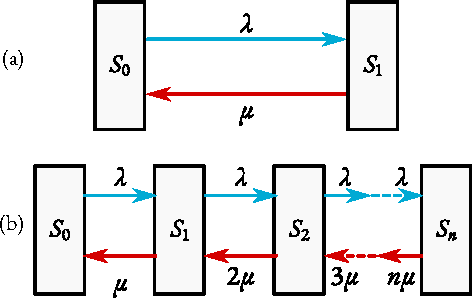
\includegraphics[width=0.75\tfwidth]{figures/state-graph3.pdf}
\caption{State graph of a system with losses.\label{state-graph3}}
 \end{figure}

We shall not go into detail on this type of system and go straight over
to a re general case, an \redem{n-server system with losses}. An example is
a system consisting of $n$ telephone lines. Erlang, the founder of the
queueing theory, considered precisely this system. The corresponding
state graph is given in \figr{state-graph3}~\drkgry{(b)}. The states of the system are designated as follows: $S_{0}$ when all servers are unoccupied, $S_{1}$ when one server is occupied and the others are unoccupied, $S_{2}$, when two servers are occupied while the others are unoccupied, and so on, and $S_{n}$ is the state
when all $n$ servers are occupied. As in the preceding example, $\lambda$ is the customer arrival rate, and $\mu$ is the service-completion rate.

Suppose the system is in state $S_{0}$. When a customer request arrives,
one of the servers becomes occupied, and the system is transferred to
state $S_{1}$. If the system is in state $S_{1}$, and a new customer arrives, two
servers become occupied, and the system is transferred from $S_{1}$ to $S_{2}$.
Thus, each customer (with the rate of arrivals $\lambda$) transfers the system
from one state to the adjacent one \redem{from left to right} (see the state graph
in the figure). The arrival of events leading to transitions to adjacent
states \redem{from right to left} is somewhat more complicated. If the system is
in the state $S_{1}$ (only one server is occupied), the next service-completion
event will disengage the server and transfer the system to state $S_{0}$. Let
me remind you that the service-completion rate is $\mu$. Now suppose the
system is in $S_{1}$, i.e. two servers are occupied. The average time of service
for each server is the same. Each sewer is disengaged with the rate
it when services are completed. As to the transition of the system from
$S_{2}$ to $S_{1}$, it is indifferent as to which of the two servers is unoccupied.
Therefore. events which transfer the system from $S_{2}$ to $S_{1}$ arrive at the
rate $2\mu$. As to the transition of the system from $S_{3}$ to $S_{2}$, it is indifferent as to which of the three occupied servers is disengaged. Events which
transfer the system from $S_{3}$ to $S_{2}$ arrive at the rate $3\mu$, and so forth. It is easy to see that the rate of event arrival which transfers the system from $S_{k}$ to $S_{k-1}$ is $k \mu$.

Let us assume that the system is in a steady state. Applying the rule
from the preceding section and using the state graph in \figr{state-graph3}~\drkgry{(b)}, we can compile the Chapman-Kolmogorov equations for the, probabilities $p_{0}, \, p_{1}, \, p_{2},\ldots{} p_{n}$, (recall that $p_{i}$ is the probability that the system is in the state $S_{i}$). We obtain the following system of equations:\\[-10pt]
\begin{equation}%
\left.
\begin{split}
\lambda p_{0} & = \mu p_{1},\\[-3pt]
(\lambda + \mu) p_{1} & = \lambda p_{0} + 2\mu p_{2},\\[-3pt]
(\lambda + 2 \mu) p_{2} & = \lambda p_{1} + 3\mu p_{3},\\[-3pt]
\ldots{} \quad \ldots{} \quad \ldots{} \quad \ldots{} , \\[-3pt]
(\lambda + k \mu) p_{k} & = \lambda p_{k-1} + (k+1)\mu p_{k+1},\\[-3pt]
\ldots{} \quad \ldots{} \quad \ldots{} \quad \ldots{} ,\\[-3pt]
[\lambda + (n-1) \mu] p_{n-1} & = \lambda p_{n-2} + n \mu p_{n},\\[-3pt]
p_{0} + p_{1} + p_{2} + \ldots{} + p_{n} & = 1.
\end{split}
\right\}
\label{eq-2.3}
%eq 2.3
\end{equation}
This set of equations can be solved easily, Using the first equation, we
can express $p_{1}$ in terms of $p_{0}$ and substitute it into the second equation. Then we can express $p_{2}$ in the second equation in terms of $p_{n}$ and substitute it into the third one, and so forth. At the last but one stage,
we express $p_{n}$ in terms of $p_{0}$. And finally, the results obtained at each
stage can be substituted into the last equation to find the expression for
$p_{0}$. Thus
\begin{equation}%
\begin{split}
p_{0} & =\left[ 1 + \frac{\lambda}{\mu} + \frac{(\lambda/\mu)^{2}}{2!}+ \frac{(\lambda/\mu)^{3}}{3!}+ \ldots + \frac{\frac{(\lambda/\mu)^{n}}{n!}}{} \right]^{-1},\\
p_{k} & = \frac{(\lambda/\mu)^{k}}{k!} p_{0} \,\, (k= 1,\, 2, \, 3 \, n).
\end{split}
\label{eq-2.4}
\end{equation}
A customer’s request is refused if it arrives when all $n$ servers are engaged, i.e. when the system is in state $S_{n}$. The probability that the system
is in $S_{n}$ equals $p_{n}$, This is the probability that a customer arriving at the system is refused and the service‘is not rendered. We can find the
probability that a customer arriving at the system will he served,
\begin{equation}%
Q = 1 - p_{n} = 1 - \frac{(\lambda/\mu)^{n}}{n!}\, p_{0}.
\label{eq-2.5}
%eq(2.5)
\end{equation}
By multiplying $Q$ by $\lambda$, we obtain the service-completion rate of the
system. Each occupied server serves $\mu$ customers per unit time, so we
can divide $Q$ by $\mu$ and find the average number of occupied servers in
the system,
\begin{equation}%
E(N) = \frac{\lambda}{\mu} \left( 1 - \frac{(\lambda/\mu)^{n}}{n!}  p_{0} \right).
\label{eq-2.6}
%eq(2.6)
\end{equation}

\txthead{How many servers are required?} Let us consider a concrete example.
Suppose a telephone exchange receives 1.5 requests per minute on the
average, and the service completion rate is 0.5 request per minute (the average service time for one customer is two minutes). Therefore, $\lambda/\mu = 3$. Suppose the exchange has three servers (three telephone lines). Using formulas \eqref{eq-2.4}--\eqref{eq-2.6} for $\lambda/\mu = 3$ and $n = 3$, we can calculate that the probability of servicing the arriving customers is only 65 per cent. The average number of engaged lines is 1.96, which is 65 per cent of the total number of lines. Thus, 35 per cent of the customers are refused and not served. This is too much. 

We may decide on increasing the number of servers. Suppose we add one more, a fourth line. Now the probability of a customer being served increases to 79 per cent (the probability of being turned away decreases to 21 per cent). The average number of engaged lines becomes 2.38, which is 60 per cent of the total number of lines. It would appear that the decision to install a fourth line is reasonable because a relatively small reduction in the percentage of occupied servers (from 65 to 60 per cent) results in a significant rise in the probability to be served, from 65 to 79 per cent. Any further increase in the number of lines may become unprofitable because the effectiveness of the system may fall due to the increasing idleness of the lines. A more detailed analysis would then be required to allow for the cost of installing each new line. Let me remark that at $n = 5$ we get $Q= 89$ per cent and $E(N)/n = 53$ per cent, while for $n= 6, \, Q= 94$ per cent and $E (N)/n = 47$ per cent.

\txthead{Single-server systems with finite queues.} Suppose	the	number of queueing customers is restricted, and the queue may only accommodate $m$ customers. If all places in the queue are occupied, a newcomer is turned away. For example, a petrol station with only one pump (only one server) and a parking area for no more than $m$ cars. If all the places at the station are occupied, the next car arriving at the station will not stop and will go on to the next.
 \begin{figure}[!h]
 \centering
 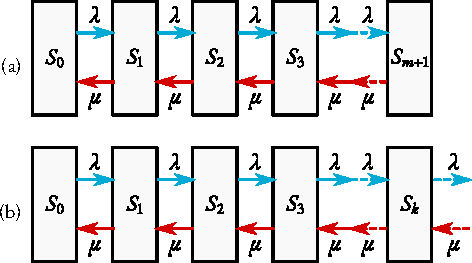
\includegraphics[width=0.75\tfwidth]{figures/state-graph4.pdf}
\caption{State graph for a system (a) with finite queues and (b) with infinite queues.\label{state-graph4}}
%fig 2.4
 \end{figure}
The state graph for this system is shown in \figr{state-graph4}~\drkgry{(a)}. Here $S_{0}$ means the server is unoccupied, $S_{1}$  the server is occupied, $S_{2}$  the server is occupied and there is one customer in the queue, $S_{3}$ the server is occupied and there are two customers in the queue, $\ldots{}, S_{m+1}$ means the server is occupied and there are $m$ customers in the queue. As before, $\lambda$ is the customer arrival rate and $\mu$ is the service completion rate. The Chapman-Kolmogorov equations for steady state are
\begin{equation}%
\left.
\begin{split}
\lambda p_{0} & = \mu p_{1},\\
(\lambda + \mu) p_{1} & = \lambda p_{0} + 2\mu p_{2},\\
\ldots{} \quad \ldots{} \quad & \ldots{} \quad \ldots{} , \\
(\lambda + \mu) p_{m} & = \lambda p_{m-1} + \mu p_{m+1},\\
p_{0} + p_{1} + p_{2} + \ldots + p_{m} + p_{m+1} & = 1.
\end{split}
\right\}
\label{eq-2.7}
%eq 2.7
\end{equation}
By solving this system and introducing the designation $\rho = \lambda/\mu$ we obtain
\begin{equation}%
p_{0} = \frac{1}{1 + \rho+ \rho^{2}+ \rho^{3}+ \ldots + \rho^{m+1}} = \frac{1 - \rho}{1 - \rho^{m+2}}, \quad  p_{k}= \rho^{k} p_{0}.
\label{eq-2.8}
%eq2.8
\end{equation}
A customer is turned away if the server is engaged and there are $m$ customers in the queue, i.e. when the system is in the state $S_{m+1}$. Therefore, the probability a customer is turned away is $p_{m+1}$. The average number of customers in the queue is evidently
\begin{equation*}%
E(r) = \sum_{k=1}^{m} k p_{k+1}
\end{equation*}
($p_{k+1}$ is the probability of $k$ customers being in the queue). The average
waiting time in the queue is the ratio $E (r)/\lambda$.

Suppose one car arrives at the petrol station per minute ($\lambda = 1$
customer per minute) and a car is filled, on average, within two minutes
$(\mu= 1/2)$. Therefore, $p = \lambda/\mu = 2$. If the number of places in the queue $m = 3$, it is easy to calculate that the probability of a customer being
refused is 51.6 per cent while the average waiting time in the queue is
2.1 min. Suppose that in order to decrease the probability of a customer
being refused we double the number of places in the queue. It turns out
that at $m = 6$ the probability of refusal is 50.2 per cent, i. e. it is, in fact, the same, but the waiting time in the queue noticeably increases to
5 min. It is clear from \eqref{eq-2.8} that if $\rho > 1$, the probability of being refused stabilizes with increasing $m$ and tends, to $(\rho - 1)/\rho$. In order to reduce the probability of being refused significantly, it is necessary (if it is not possible to decrease $\rho$) to use multi-server systems.

\txthead{Single-server systems with infinite queues.} This sort of queueing
system is rather common: for example, a doctor receiving patients,
a single public telephone, or a port with only one berth at which
a single ship can unload. The state graph for the system is given in
\figr{state-graph4}~\drkgry{(b)}. Here So means that the server is unoccupied, $S_{1}$ the server is occupied, $S_{2}$ the server is occupied and there is one customer in the queue, $S_{3}$ the server is occupied and there are two customers in the queue, and $S_{k}$ means that the server is occupied and there are $k - 1$
customers in the queue, and so on.

Up till now, we considered graphs with a finite number of states. However, here is a system with an infinite number of discrete states. Is it possible to discuss a steady state for such a system? In fact we can. It is only necessary that the inequality $\rho < 1$ holds true. If so, then the sum
$1 + \rho+ \rho^{2}+ \rho^{3}+ \ldots{} + \rho^{m+1}$ in \eqref{eq-2.8} can be substituted by the sum of the decreasing geometric progression $1 + \rho+ \rho^{2}+ \rho^{3}+ \ldots{}  = 1/(1 - \rho)$. The result is
\begin{equation}%
p_{0} = 1 - \rho  \qand  p_{k} = \rho^{k} p_{0}.
\label{eq-2.9}
\end{equation}
If $\rho \geqslant 1$, then the system does not have a steady state, i.e. the queue increases infinitely as $t \to \infty$.

\section{Method of Statistical Testing}

A \redem{statistical testing} involves numerous repetitions of uniform trials. The
result of any individual trial is random and is not of much interest.
However, a large number of results is very useful. It shows some
stability (\redem{statistical stability}) and so the phenomenon being investigated
in the trials can be described quantitatively. Let us consider a special
method for investigating a random process based on statistical testing.
The technique is commonly called the \redem{Monte Carlo method}.

In fact neither the city of Monte Carlo, the capital of the independent
principality of Monaco nor its inhabitants nor guests are in any way
related to the considered method. Instead, the city is known for its
casinos where tourists pay good money playing roulette, and a roulette
wheel could be the city's emblem. At the same time, a roulette is
a generator of random numbers and this is what is involved when the
Monte Carlo method is used.

\txthead{Two examples indicating the usefulness of statistical testing.} 

\redem{First example.} Look at \figr{monte-carlo1}. It contains a square with side $r$ in which a quarter circle of radius $r$ is inscribed. The ratio of the yellow area to the area of the square is $(\pi r^{2})/4r^{2} = \pi /4$. This ratio and, therefore, the value of $n$ can be obtained using the following statistical test. Let us place a sheet of paper with the figure on a horizontal surface and let us throw small grains on this paper. We should not aim so that any grain
can fall on any part of the paper with equal probability. It is possible,
for instance, to blindfold the person throwing the grains. The grains will
be distributed over the surface of the paper in a random fashion
(\figr{monte-carlo1}~\drkgry{(b)}). Some will land outside the square, but we shall not consider them. We now count the number of grains within the square (and call
this number $N_{1}$) and count the grains within the yellow area (calling it
$N_{2}$). Since any grain may land with equal probability on any part of the
figure, the ratio $N_{2}/N_{1}$ when the number of trials is large, will
approximate the ratio of the yellow area to the area of the square, i.e.
the number $\pi /4$. This approximation will become more accurate as the
number of trials increases.
 \begin{figure}[!h]
 \centering
 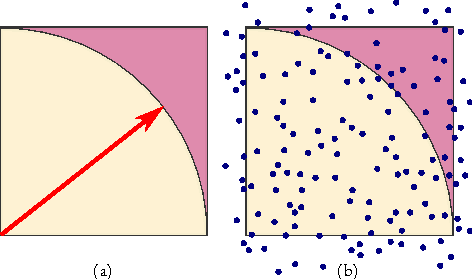
\includegraphics[width=0.85\tfwidth]{figures/monte-carlo1.pdf}
\caption{Finding out value of $\pi$ using a random distribution.\label{monte-carlo1}}
%fig 2.6
 \end{figure}
This example is interesting because a definite number (the number $\pi$)
can be found following a statistical testing. It can be said that
randomness is used here to obtain a deterministic result, an
approximation of the real number $\pi$.


\redem{Second example}. Statistical testing is used much more commonly to
investigate \redem{random events} and \redem{random processes}. Suppose someone
assembles a device consisting of three parts ($A$, $B$, and $C$). The assembler
has three boxes containing parts $A$, $B$, and $C$, respectively. Suppose half
the parts of each type are larger than the standard and the other half
are smaller. The device cannot operate when all three parts are larger
than the norm. The assembler takes the parts from the boxes at random.
What is the probability that a normally operating device will be
assembled?

Naturally, this example is rather simple and the probability can easily
be calculated. The probability of assembling a device that does not work
is the probability that all three parts will be larger than the norm, and
this equals $1/2 \times 1/2 \times 1/2 = 1/8$. Therefore, the probability that
a normally operating device will be assembled is $1 - 1/8 = 0.875$.

Let us forget for a time that we can calculate the probability and
instead use statistical testing. We should choose trials such that each
one has equally probable outcomes, for instance, tossing a coin. Let us
take three coins: $A$, $B$, and $C$. Each coin corresponds to a part used to
assemble the device. Heads will mean that the respective part is larger
than the norm while tails will mean that it is smaller. Having agreed on
this, let us start the statistical testing. Each trial involves tossing all
three coins. Suppose after $N$ trials ($N \gg 1$) three heads were recorded in
$n$ trials. It is easy to see that the ratio $(N - n)/N$ is the approximation of
the probability in question.

Naturally, we could use any other random number generator instead
of coins. It would also be possible, for instance, to throw three dice,
having agreed to relate three faces of each die with larger than normal
parts and three faces with smaller parts.

Let me emphasize that the randomness in these examples was
a positive factor rather than a negative one, and was a tool which
allowed us to obtain a needed quantity. Here chance works for us rather
than against us.

\txthead{Random number tables come into play.} Nobody uses statistical
testing in simple practical situations like the ones described above. It is
used when it is difficult or even impossible to calculate the probability
in question. Naturally you might ask whether a statistical testing would
be too complicated and cumbersome. We threw grains or three coins in
the examples. What will be required in complicated situations? Maybe,
there will be practically unsurmountable obstacles?

In reality, it is not necessary to stage a statistical experiment with
random trials. Instead of real trials (throwing grains, dice, etc.), we need
only use \redem{random number tables}. Let me show how this can be done in
the above two examples.
 \begin{figure}[!h]
 \centering
 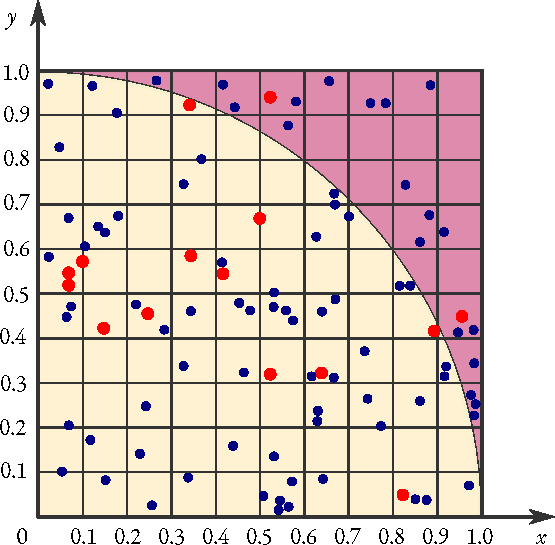
\includegraphics[width=0.75\textwidth]{figures/monte-carlo2.pdf}
\caption{Finding out value of $\pi$ using a random number table.\label{monte-carlo2}}
%fig 2.7
 \end{figure}
 
\redem{First example.} Let us again discuss the picture in \figr{monte-carlo1}. We now plot two coordinate axes along the sides of the square and select the scales such that the side of the square equals unity (\figr{monte-carlo2}). Now instead of throwing grains, we take the random number table in \figr{random-table} and divide each number by \num{10000} so that we obtain a set of random numbers between 0 and 1. We take the numbers in the odd lines as $x$-coordinates and the ones directly below as the $y$-coordinates of random points. We plot the points onto the diagram, systematically
moving along the random number table (for instance, first down the first
column from top to bottom, and then down the second column, and so
on). The first fifteen random points are shown in the picture in red, and
they have the coordinates as shown in \tabl{random-coord}.%\\[-15pt]
\begin{wrapfloat}{table}{O}{\mfwidth}
\centering
\begin{smaller}
\begin{tabular}{l}
(0.0655, 0.5255) \\
 (0.6314, 0.3157) \\
  (0.9052, 0.4105) \\
(0.1437, 0.4064) \\
 (0.1037, 0.5718) \\
  (0.5127, 0.9401) \\
(0.4064, 0.5458) \\ 
(0.2461, 0.4320) \\ 
(0.3466, 0.9313) \\ 
(0.5179, 0.3010) \\ 
(0.9599, 0.4242) \\
 (0.3585, 0.5950) \\ 
(0.8462, 0.0456) \\
 (0.0672, 0.5163) \\
  (0.4995, 0.6751) \\
\end{tabular}
\end{smaller}
%\end{center}
\caption{Coordinates of fifteen random numbers shown in red in the \figr{monte-carlo2}. \label{random-coord}}
\end{wrapfloat}
The figure contains 85 random points in black. From
the diagram, it is easy to calculate that using the first fifteen points
$N_{2}/N_{1}= 13/15$ and therefore $\pi = 3.47$ while for a hundred points
$N_{2}/N_{1}= 78/100$ and therefore $\pi = 3.12$.

\redem{Second example.} Instead of tossing coins, we can use the same random
number table (see \figr{random-table}). Each number over \num{5000} can be replaced by a ``+'' sign and the rest replaced by a ``$-$'' sign. The result is a table
consisting of a random set of pluses and minuses. We divide these signs
into triples as shown in \figr{monte-carlo3}. Each triple corresponds to a set of three parts. A ``+'' sign means that a part is larger than the norm while
a ``$-$'' sign means it is smaller. The approximation of the sought
probability is the ratio $(N - n)/N$, where $N$ is the total number of triples
and $n$ is the number of triples with three pluses (they are shaded in the
figure). It can be seen that $(N - n)/N = 0.9$ in this case, and this is close
enough to the accurate value 0.875.
 \begin{figure}[!h]
 \centering
 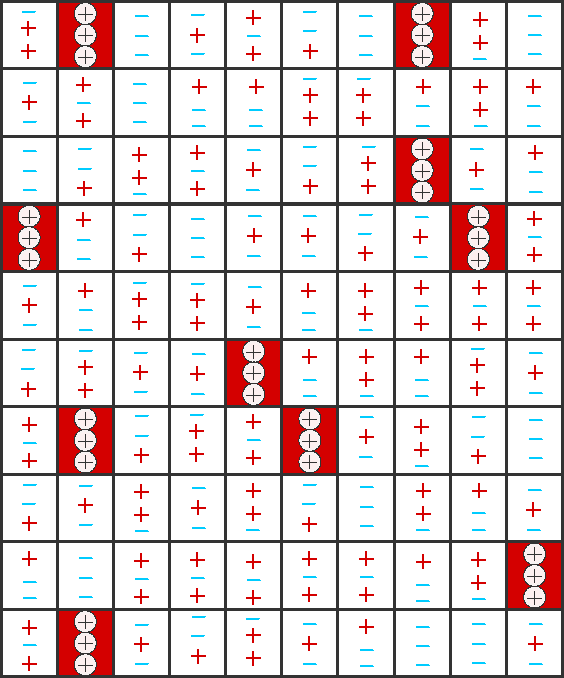
\includegraphics[width=0.75\tfwidth]{figures/monte-carlo3.pdf}
\caption{Using a random number table instead of coin tosses for statistical testing.\label{monte-carlo3}}
%fig 2.7
 \end{figure}

Thus, we have reduced statistical testing to operations on a random
number table and used our desk instead of an experimental bench.
Rather than performing very many trials, we just look at a random
number table.

\txthead{Computers come into play.} Instead of sweating over a random
number table, we could program a computer to do the job. We place
a random number table in the computer's memory and program it to
search the random numbers and sort them as necessary. In our two
examples, we would do the following.

\redem{First example}. The computer has to check the coordinates of each
random point to see whether $x^{2} + y^{2} < 1$. It counts the number of points
for which this is true (the number is $N_{2}$) and the number of points for
which it is false (this number of points will be the difference $N_{1} - N_{2}$).

\redem{Second example}. All random numbers in the computer's memory must
be divided into triples and the triples checked to find ones in which all three numbers are over 5000. The number of such triples is $n$.

\txthead{The Monte Carlo method.} The world changed when the computer
came into play. By processing a random number table the computer
simulates the statistical testing and it can do this many times faster than
could be done either experimentally or by working manually with
a random number table. And now we come to the Monte Carlo method,
a very useful and efficient method of probabilistic calculation which is
applied to many problems, primarily those that cannot be solved
analytically.

Let me emphasize two points. \redem{Firstly}, the Monte Carlo method
utilizes \redem{randomness not chance}. We do not try to analyze the complicated random processes, nor even simulate them. Instead, we use randomness, as it were, to deal with the complications chance has engendered.

Chance complicates our investigation and so randomness is used to
investigate it. \redem{Secondly}, this method is \redem{universal} because it is not restricted by any assumption, simplification, or model. There are two
basic applications. The first is the investigation of random processes
which cannot be dealt with analytically due to their complexity. The
second is to verify the correctness and accuracy of an analytical model
applied in concrete situations.

The Monte Carlo method was first widely used in operations research,
in looking for optimal decisions under conditions of uncertainty, and in
treating complicated multi-criterial problems. The method is also successfully
used in modern physics to investigate complex processes involving
many random events.

\txthead{A Monte Carlo simulation of a physical process.} Let us consider the
flow of neutrons through the containment shield of a nuclear reactor.
Uranium nuclei split in the core of the reactor and this is accompanied
by the creation of high-energy neutrons (of the order of several million
electron volts). The reactor is surrounded by a shield to protect the
working areas (and therefore, the personnel) from the radiation. The
wall is bombarded by an intense flow of neutrons from the reactor core.
The neutrons penetrate into the wall and collide with the nuclei of the
atoms of the wall. The result is that the neutrons may either be
absorbed or scattered. If scattered, they give up some of their energy to
the scattering nuclei.

This is a complicated physical process \redem{involving many random events}.
The energy and the direction of a neutron when it leaves the reactor
core and enters the wall are random, the length of the neutron path
before it first collides is random, the nature of collision (absorption or
scattering) is random, the energy and the direction of the scattered
neutron are random, etc. Let me show in general how the Monte Carlo
method is applied to analyze the process. Obviously the computer is
first programmed with data on the elementary collisions between
neutrons and the wall nuclei (the probabilities of absorption and
scattering) the parameters of the neutron flow into the wall, and the
properties of the wall. The computer model simulates a neutron with
a randomly selected energy and direction (when it leaves the reactor
core and enters the wall) in line with appropriate probabilities. Then it
simulates (bearing in mind the relevant probabilities) the flight of the
neutron until it first collides. Then the first collision is simulated. If the
neutron is not absorbed, subsequent events are simulated, i.e. the
neutron's flight until its second collision, the collision itself, and so on.
The ``history'' of the neutron is determined from the moment it
penetrates the wall until it is either absorbed, scattered back into the
reactor core, or scattered into the working area. 

The computer simulation is repeated for very many neutrons until a set of possible
trajectories of neutrons within the wall is obtained (\figr{neutron-path}). Each trajectory is the result of one statistical trial simulating the ``history'' of
Chance complicates our investigation and so randomness is used to
investigate it. Secondly, this method is universal because it is not
restricted by any assumption, simplification, or model. There are two
an individual neutron. Given an enormous set of trials the neutron flow
through the containment wall as a whole can be analyzed and
recommendations for the thickness of the wall and its composition can
be made so as to guarantee the safety of the personnel working at the
reactor.
 \begin{figure}[!h]
 \centering
 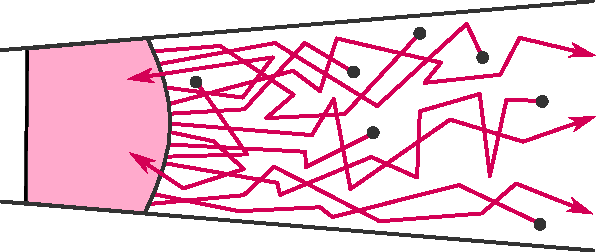
\includegraphics[width=0.85\tfwidth]{figures/neutron-path.pdf}
\caption{A set of all possible trajectories for the neutron.\label{neutron-path}}
%fig 2.9
 \end{figure}

Modern physics requires the Monte Carlo method on many
occasions. Physicists use it to investigate cosmic-ray showers in the
Earth's atmosphere, the behaviour of large flows of electrons in electron
discharge devices, and the progress of various chain reactions.

\section{Games and Decision Making}

\txthead{What is the theory of games?} Suppose we must make a decision when
our objectives are opposed by another party, when our will is in conflict
with another will. Such situations are common, and they are called
\redem{conflict situations}. They are typical for military actions, games, and
every-day life. They often arise in economics and politics.

A hockey player makes a decision that takes into account the current
situation and the possible actions of the other players. Every time
a chess player makes a decision, he (or she) has to consider the
counteraction of the opponent. A military decision should allow for the
retaliation of the enemy. In order to decide at what price to sell
a product, a salesman must think over the responses of the buyer. In
any election campaign, each political party in a capitalist country tries
to foresee the actions of the other parties that are competing for power.
In each case, there is a collision of opposing interests, and the decision
must be related with \redem{overcoming a conflict}.

Decision making in a conflict situation is hampered by \redem{uncertainty
about the behaviour of the opponent}. We know that the opponent will try
to act in a way that is least advantageous for us in order to ensure the
greatest advantage for himself. However, we do not know to what extent
our opponent is able to evaluate the situation and the possible
consequences and, in particular, how he evaluates our options and
intentions. We cannot predict the actions of the opponent accurately,
and the opponent cannot predict our actions. But nonetheless, we both
have to make decisions.

Because some way of justifying an \redem{optimal} decision was needed in
conflict situations, a new mathematical discipline arose, the \redem{theory of
games}. The ``game'' here is a mathematical model of a conflict situation.
Unlike a real conflict, a game has definite rules which clearly indicate
the rights and duties of the participants and the possible outcomes of
the game (a gain or loss for each participant). Long before the
emergence of game theory, simple models of conflicts were used widely.
I mean games in the literal sense of the word: chess, checkers or
draughts, dominoes, card games, etc. In fact, the name of the theory and
the various terms used in it are all derived from these simple models.
For instance, the conflicting parties are called players, a realization of
a game is a match, the selection of an action by a player (within the
rules) is a move.

There are two kinds of move, personal and chance ones. A \redem{personal}
move is when the player conscientiously selects an action according to
the rules of the game. A \redem{chance} move does not depend on the player's
will: it may be determined by tossing a coin, throwing a die, taking
a card from a pack, etc. Games consisting of only chance moves are
called \redem{games of chance}, or \redem{games of hazard}. Typical examples are lotteries and bingo. Games with personal moves are called \redem{strategic}.
There are strategic games consisting exclusively of personal moves, for
instance, chess. There are also strategic games consisting of both
personal and chance moves, for instance, certain card games. Let me
remark that the uncertainty in games with both personal and chance
moves involve both sorts of randomness: the uncertainty of the result of
the chance moves and the uncertainty of the opponent's behaviour in his
personal moves.

Game theory is not interested in gambles. It only deals with strategic
games. The aim of the game theory is to determine the player's strategy
so as to maximize his chances of winning. The following basic
assumption underlies the search for optimal strategies. It is assumed that
the opponent is as active and as reasonable as the player, and he or she
also takes attempts to succeed.

Naturally, this is not always true. Very often our actions in real
conflicts are not as good as they could be when we assume reasonable
behaviour from our adversary; it is often better to guess at the ``soft
spots'' of the opponent and utilize them. Of course, we take a risk when
doing so. It is risky to rely too much on the soft spots of the opponent,
and game theory does not consider risk. It only detects the most
cautious, ``safe'' versions of behaviour in a given situation. It can be said
that game theory gives wise advice. By taking this advice when we make
a practical decision, we often take a conscientious risk. E. S. Wentzel
writes in \redem{Operations Research}: 
\begin{quote}
``Game theory is primarily valuable in
terms of the formulation of the problem, which teaches us never to forget that the opponent also thinks and to take into account his possible tricks and traps. The recommendations following from the
game approach are not always concrete or realizable, but it is still
useful, while taking a decision, to utilize a game model as one of several
possible ones. But the conclusions proceeding from this model should
not be regarded as final and indisputable.''
\end{quote}

\txthead{The payoff matrix of a game} \redem{Finite two-person zero-sum games} are the best investigated types in game theory. A \redem{two-person} game is a game in which there are exactly two players or conflicting interests. A game is \redem{finite} if both players have a finite number of possible strategies, i.e. a finite number of behaviours. When making a personal move, a player
follows a strategy. A \redem{zero-sum} game is a game where the gain by one
player equals the loss by the other.

 \begin{figure}[!h]
 \centering
 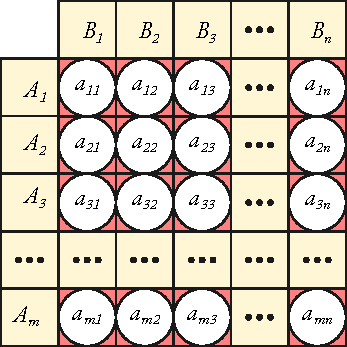
\includegraphics[width=0.6\tfwidth]{figures/two-player1.pdf}
\caption{Strategies in a finite two-person zero-sum game.\label{twoplayer1}}
%fig 2.10
 \end{figure}

Suppose there is a finite two-person zero-sum game where player
$A$ has $m$ strategies and player $B$ has $n$ strategies (an $m \times n$ game). We use $A_{1}, \, A_{2}, \ldots, A_{m}$ to denote the strategies available to player $A$ and $B_{1}, \, B_{2}, \ldots, B_{n}$ the strategies available to player $B$. Suppose player $A$ makes a personal move and selects a strategy $A_{i} (1 \leqslant i \leqslant m)$, and player $B$ at the same time selects strategy $B_{j} (1 \leqslant j \leqslant n)$. We use $a_{ij}$ to denote the gain of player $A$. Let us identify ourselves with player $A$ and consider each move from his viewpoint. The gain $a_{ij}$ may be either a real gain or a loss (a loss would be a negative gain). The set of gains $a_{ij}$ for different values of $i$ and $j$ can be arranged in matrix form with the rows corresponding to player $A$ strategies and the columns to player $B$ strategies (\figr{twoplayer1}). This is called the \redem{payoff matrix} for the game.

Consider the following game. Each player, $A$ and $B$, writes, simultaneously
and independently, one of three numbers 1, 2, or 3. If the sum of
the numbers is \redem{even}, player $B$ pays player $A$ the sum, while if the sum is \redem{odd}, $A$ pays it to $B$. Player $A$ has three strategies: $A_{1}$ to write 1, $A_{2}$ to write 2, and $A_{3}$ to write 3. Player $B$ has the same strategies. The game is a $3 \times 3$ one because its payoff matrix contains three rows and three columns. This matrix is given in Figure \ref{twoplayer2}(a). Note that a gain by player $A$ of, for instance, $-3$ is a loss in reality because $A$ pays 3 units to $B$. 

 \begin{figure}[!h]
 \centering
 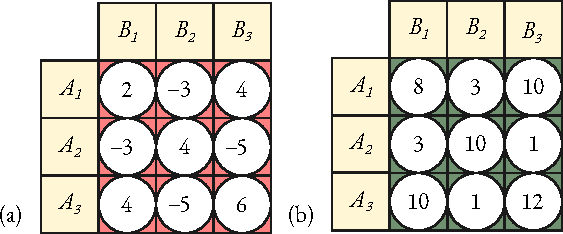
\includegraphics[width=0.85\tfwidth]{figures/two-player2.pdf}
\caption{A payoff matrix in a $3 \times 3$ finite two-person zero-sum game.\label{twoplayer2}}
%fig 2.11
 \end{figure}


Some of the elements are positive and the others are negative in the matrix in Figure \ref{twoplayer2}(a). It is possible to make all the elements of the payoff matrix positive by adding some number, say 6, to each element of the
matrix. We obtain the matrix in Figure \ref{twoplayer2}(b). This matrix is equivalent to the initial one from the viewpoint of analyzing optimal strategies.

\txthead{The minimax principle} Let us analyze the game using. the payoff
matrix in \figr{twoplayer2}(b). Suppose we (player $A$) pick strategy $A_{i}$. Then, depending on the strategy selected by player $B$, our gain may be either 8 or 3 or 10. Thus, strategy $A_{1}$ yields a gain of 3 in the worst case. If we choose either $A_{2}$ or $A_{3}$, the worst gain is 1. Let us write down the
minimum possible gains for each strategy $A_{i}$ as an additional column in
the payoff matrix (\figr{twoplayer3}). It is clear that we should choose a strategy whose \redem{minimum possible gain is greatest} (as compared with the other strategies). This is strategy $A_{1}$ in this case. Three is the largest one out of the minimum gains for each strategy (viz. 3, 1, and 1). This is called
the \redem{maximin gain}, or the \redem{maximin}, or just the \redem{maxim}. It is also sometimes called the \redem{lower value of the gain}. Thus, if we select the maximin strategy (strategy $A_{1}$ in this case), our gain is guaranteed to be, whatever the behaviour of the opponent, at least the lower value of the game (a gain of 3 in this case). The opponent will reason in a similar way. If he selects
strategy $B_{1}$, he will have to give us a gain of 10, which is his worst case.

 \begin{wrapfigure}{O}{\mfwidth}
 \centering
 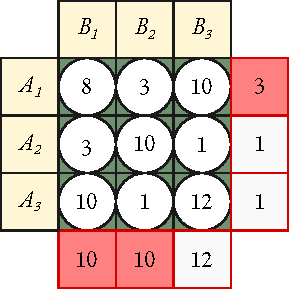
\includegraphics[width=0.9\linewidth]{figures/two-player3.pdf}
\caption{A payoff matrix in a $3 \times 3$ finite two-person zero-sum game.\label{twoplayer3}}
%fig 2.12
 \end{wrapfigure}
The same can be said of strategy $B_{2}$. Strategy $B_{3}$ yields the worst case
for the opponent corresponding to a gain of 12 for us. Numbers 10, 10,
and 12 are the maximum values of our gains corresponding to the
opponent's strategies $B_{1}$, $B_{2}$, and $B_{3}$, respectively. Let us write these values as a row in the payoff matrix (see \figr{twoplayer3}). It is clear that our opponent should select the strategy which \redem{minimizes} our \redem{maximum possible gain}. This is either strategy $B_{1}$ or $B_{2}$. Both strategies are minimax ones and both guarantee that our opponent limits our gain to the \redem{minimax}, or, in other words, the \redem{upper value of the game} is 10.

Our maximin strategy and the minimax strategy of the opponent are
the most cautious ``safe'' strategies. The principle of being cautious
dictating that the players select such strategies is called the \redem{minimax
principle}.

Now let us return to the matrix in \figr{twoplayer3} and try some reasoning. The opponent has two minimax strategies,  $B_{1}$ and  $B_{2}$. Which strategy should he choose? If he knows that we are cautious and have selected the maximin strategy  $A_{1}$ he would not select strategy  $B_{1}$ because this would yield a gain of 8. Therefore, it is likely that he would choose
strategy $B_{2}$, and our gain would then be 3. But if we perceived our
opponent's ideas correctly, shouldn't we take a risk and choose strategy
 $A_{2}$? If the opponent then selects strategy  $B_{2}$, our strategy  $A_{2}$ will give us a gain of 10. However, our deviation from the minimax principle may
cost us dearly. If the opponent is even cleverer and reasons in a similar
way, he would answer our strategy  $A_{2}$ with strategy  $B_{3}$ rather than  $B_{2}$. And then, instead of a gain of 10, we would only gain 1.

Does this mean that game theory only recommends we adhere to
a minimax (maximin) strategy? It depends on whether the payoff matrix
has a \redem{saddle point}.

\txthead{A game with a saddle point.} Consider the $3 \times 3$ game, whose payoff matrix is given in \figr{saddle-point}. Here both the maximin and minimax gain 4. In other words, the lower and the upper value of the game coincide and both are equal to 4. A gain of 4 is simultaneously the maximum of
the minimum gains for strategies $A_{1}, \, A_{2}$, and $A_{3}$ and the minimum of the maximum gains for strategies $B_{1}, \, B_{2}$, and $B_{3}$. In geometry, the point on a surface which is at the same time a minimum along one coordinate axis and a maximum along the other is called a saddle point. Point $C$ on the surface in \figr{saddle-point} is a \redem{saddle point}. It is the maximum along the $x$-axis and the minimum along the $y$-axis. It is easy to see that the surface in the vicinity of this point is actually like a saddle. Just as in geometry, element $a_{22} = 4$ of the payoff matrix in question is called the
\redem{saddle point of the matrix}, and the game is said to have a saddle point.

 \begin{figure}[!h]
 \centering
 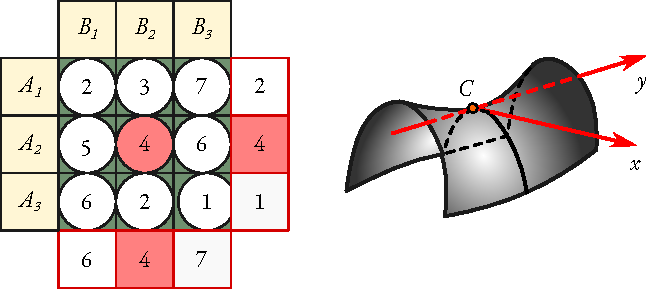
\includegraphics[width=\tfwidth]{figures/saddle-point.pdf}
\caption{A $3 \times 3$ game with saddle point.\label{saddle-point}}
%fig 2.13
 \end{figure}
We need only look through the matrix in \figr{saddle-point}, to see that each player should adhere to his maximin (minimax) strategy. These strategies
are optimal in a game with a saddle point. Any deviation from them will
be disadvantageous for the player who took the risk.

However, if a game does not have a saddle point (see the matrix in
\figr{twoplayer2}), neither of strategies $A_{i}$ or $B_{j}$ is optimal.

\txthead{The necessity of a random change of strategy in a game without
a saddle point.} Suppose that we and our opponent repeatedly play the
game whose matrix is given in \figr{twoplayer2}. If we choose a definite strategy, for instance, the maximin strategy $A_{1}$, and adhere to it turn after turn, our opponent will see it and select strategy $B_{2}$ each time, so that our
gain will not exceed the lower value of the game, i.e. it will equal 3.
However, if we suddenly (for the opponent) choose strategy $A_{2}$ instead
of $A_{1}$, we receive a gain of 10. Having guessed our new strategy
(naturally, if we later adhere to it), our opponent will go from strategy
$B_{2}$ to strategy $B_{3}$ right away, thus decreasing our gain to 1. And so
forth. We can see here a general rule for games without a saddle point:
a player using a \redem{certain strategy} will be worse off than a player who
\redem{changes strategy at random}.

However, the random changes in strategies should be done wisely
rather than haphazardly. Suppose $A_{1}, \, A_{2}, \ldots, A_{m}$ are the possible
strategies of player $A$ (see \figr{twoplayer1}). To obtain the greatest benefit, the strategies should be chosen at random but with different (specially
calculated) probabilities. Suppose strategy $A_{1}$ is used with probability
$p_{1}$, strategy $A_{2}$ with probability $p_{2}$ etc. Player $A$ is now said to have a \redem{mixed strategy} $S_{A} (p_{1}, \, p_{2}, \ldots{}, p_{m})$. Unlike $S_{A}$, the $A_{j}$ strategies are called \redem{pure strategies}. By correctly selecting the probabilities $p_{j}$ a mixed strategy may be \redem{optimal}. The gain of player $A$ will then be no less than a certain value $\nu$ called the \redem{value of the game}. This value is greater than the lower value of the game, but less than the upper one.

Player $B$ should behave in a similar manner. His optimal strategy is
also a mixed strategy. Let us designate it  $S_{B} (q_{1}, \, q_{2}, \ldots{}, q_{n})$, where $q_{j}$ are specially selected probabilities with which player $B$ uses strategies $B_{j}$. When player $B$ selects an optimal mixed strategy, the gain of player $A$ will be no more than game value $\nu$.

\txthead{The search for an optimal mixed strategy.} Let us use $S_{A} (p_{1}, \, p_{2}, \ldots{}, p_{m})$ to denote an optimal mixed strategy for player $A$. We must now find probabilities $p_{1}, \, p_{2}, \ldots{}, p_{m}$ and calculate the game value $\nu$ once the payoff matrix of the game is known (see \figr{twoplayer1}). Suppose player $B$ selects pure strategy $B_{1}$. Then the average gain of player $A$ will be $a_{11}p_{1} + a_{21}p_{2}+ \ldots{} + a_{m1}p_{m}$ This gain should be no less than the game value $\nu$, and hence
\begin{equation*}%
a_{11}p_{1} + a_{21}p_{2}+ \ldots + a_{m1}p_{m} \geqslant \nu.
\end{equation*}
If player $B$ selects strategy $B_{2}$, the average gain of player $A$ should also
be no less than the game value $\nu$, and hence
\begin{equation*}%
a_{12}p_{1} + a_{22}p_{2}+ \ldots + a_{m2}p_{m} \geqslant \nu.
%\label{b-strategy2}
% eq-2.10
\end{equation*}
Whichever strategy player $B$ chooses, the gain of player $A$ should
always be no less than the game value $\nu$. Therefore, we can write the
following system of $n$ inequalities (recall that $n$ is the number of $B$'s pure
strategies):
\begin{equation}%
\left.
\begin{split}
a_{11}p_{1} + a_{21}p_{2}+ \ldots + a_{m1}p_{m} & \geqslant \nu, \\
a_{12}p_{1} + a_{22}p_{2}+ \ldots + a_{m2}p_{m} & \geqslant \nu, \\
\ldots \quad \ldots \quad \ldots  \quad \ldots, \\
a_{1n}p_{1} + a_{2n}p_{2}+ \ldots + a_{mn}p_{m} & \geqslant \nu. \\
\end{split}
\right\}
\label{eq-2.10}
%eq-2.10
\end{equation}
Recall that
\begin{equation}
p_{1} + p_{2}+ \ldots + p_{m} = 1.
\label{eq-2.11}
%eq 2.11
\end{equation}
Introducing designations $x_{1} = 	p_{1}/\nu, \, x_{2} = p_{2}/\nu, \ldots x_{m} = 	p_{m}/\nu$ we can rewrite \eqref{eq-2.10} and \eqref{eq-2.11} as
\begin{equation}%
\left.
\begin{split}
a_{11}x_{1} + a_{21}x_{2}+ \ldots + x_{m1}p_{m} & \geqslant 1, \\
a_{12}x_{1} + a_{22}x_{2}+ \ldots + a_{m2}x_{m} & \geqslant 1, \\
\ldots \quad \ldots \quad \ldots  \quad \ldots, \\
a_{1n}x_{1} + a_{2n}x_{2}+ \ldots + a_{mn}x_{m} & \geqslant 1. \\
\label{eq-2.12}
\end{split}
\right\}
%eq-2.12
\end{equation}
\begin{equation}%
x_{1} + x_{2}+ \ldots + x_{m} = \frac{1}{\nu}. 
\label{eq-2.13}
%eq 2.13
\end{equation}
It is desirable that the game value $\nu$ should be as large as possible,
and hence $1/\nu$ should be as low as possible. Therefore, the search for the
optimal mixed strategy is thus reduced to the solution of the following
mathematical problem: find non-negative values $x_{1}, \, x_{2}, \, \ldots \, x_{m}$ such that they meet inequalities \eqref{eq-2.12} and minimize the sum $x_{1} + x_{2}+ \ldots{} + x_{m}$.

 \begin{wrapfigure}{O}{\mfwidth}
 \centering
 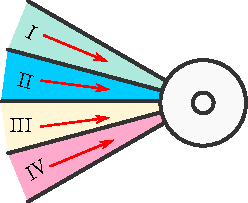
\includegraphics[width=0.9\linewidth]{figures/anti-aircraft.pdf}
\caption{Strategies with aeroplanes and anti-aircraft guns.\label{anti-aircraft}}
%fig 2.14
 \end{wrapfigure}

\txthead{Airplanes against antiaircraft guns.} Let us find the optimal mixed
strategy for a concrete game. Suppose ``player'' $A$ wants to attack
``player'' $B$. $A$ has two airplanes each carrying a large bomb. $B$ has four
antiaircraft guns defending an important military base. To destroy the
base, it is sufficient for at least one airplane to approach it. To approach
the base the airplanes may choose one of four air corridors (\figr{anti-aircraft}, where 0 is the base and I, II, III, and IV are the air corridors). $A$ may send both airplanes along the same corridor or along different corridors. $B$ may place his four antiaircraft guns to cover the corridors in different ways. Each gun can only shoot once, but it will hit the airplane if it is in that corridor.
 
$A$ has two pure strategies: strategy $A_{1}$ to send the airplanes along
different corridors (no matter which ones), and $A_{2}$, to send both
airplanes along the same corridor. $B$'s strategies are $B_{1}$ to put an
antiaircraft gun into each corridor, $B_{2}$ to put two guns into two
corridors (leaving the other two corridors unprotected), $B_{3}$ to put two
guns into one corridor and one gun into two of the other corridors, $B_{4}$
to put three guns into a corridor and one gun into another corridor,
and $B_{5}$ to put all four guns into one corridor. Strategies $B_{4}$ and $B_{5}$ are certainly bad because three or four guns in a single corridor are not
needed, since $A$ only has two airplanes. Therefore, we need only discuss
strategies $B_{1}$, $B_{2}$, and $B_{3}$.

 \begin{wrapfigure}{O}{\mfwidth}
 \centering
 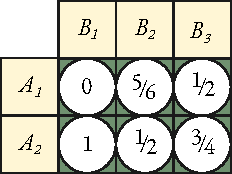
\includegraphics[width=0.7\linewidth]{figures/aa-matrix.pdf}
\caption{Matrix of probable with aeroplanes and anti-aircraft guns.\label{aa-matrix}}
%fig 2.15
 \end{wrapfigure}
Suppose $A$ chooses strategy $A_{1}$ and $B$ chooses strategy $B_{1}$. It is clear that neither airplane will reach base: the $A$'s gain will be zero ($a_{11}=0$). Suppose strategies $A_{1}$ and $B_{2}$ are chosen. Let us assume that the guns are in corridors I and II. If the aircrafts are flying along different corridors, then six variants are equally probable: they fly along corridors I and II, along corridors I and III, along corridors I and IV, along II and III, along II and IV, or along III and IV. In only one of the six cases will neither plane reach the base (when they fly along corridors I and II). Whichever corridor $B$ chooses to place his guns in, airplanes will always have six equally probable variants and only one does not yield a winning move. Therefore, if strategies $A_{1}$ and 
$B_{2}$ are chosen, the probable gain for $A$ will be 5/6 ($a_{12}$ = 5/6). Reasoning in the same manner, it is easy to find the rest of the elements of the
payoff matrix for this game. The resultant $2 \times 3$ matrix is shown in
\figr{aa-matrix}. Note that the elements of the matrix are \redem{probable} gains; so here even the pure strategies involve chance. The lower value of the
game is 1/2, and the upper one is 3/4. The maximin strategy is $A_{2}$ while
the minimax strategy is $B_{3}$. There is no saddle point, and the optimal
solution for the game will be a mixed strategy.

In order to find the optimal mixed strategy, let us use the payoff
matrix and relations \eqref{eq-2.12} and \eqref{eq-2.13}. The relations for this case are
\begin{align}%
 x_{2} \geqslant 1, \quad \frac{5}{6}x_{1} + \frac{1}{2} x_{2}  \geqslant 1, \quad  \frac{1}{2}x_{1} + \frac{3}{4} x_{2} & \geqslant 1 \label{eq-2.14},\\
x_{1} + x_{2} & = \frac{1}{\nu}. \label{eq-2.15}
\end{align}
The solution can be conveniently represented as a diagram. We plot
the positive values $x_{1}$ and $x_{2}$ along the coordinate axes (\figr{aa-graph}). The first inequality in \eqref{eq-2.14} corresponds to the area above the straight line $CC$; the second inequality is the area above $DD$; and the third inequality in \eqref{eq-2.14} is the area above $EE$. All three inequalities are satisfied inside the area shaded red in the figure. The equation $x_{1} + x_{2} = \text{const}$ defines a family of straight lines, some of which are shown in figure as dash lines. The straight line $FF$ has the least sum $x_{1} + x_{2}$ of all the lines in the family with at least one point within the red area. Point
$G$ indicates the solution corresponding to the \redem{optimal mixed strategy}.
The coordinates of this point are  $x_{1} = 3/5$ and  $x_{2} = 1$. Hence we find
$\nu = 5/8, \, p_{1} = 3/8, \, \text{and} \, p_{2} = 5/8$. Thus, $A$'s optimal mixed strategy would be to use strategy $A_{1}$ with probability 3/8 and strategy $A_{2}$ with probability 5/8.
 \begin{figure}[!h]
 \centering
 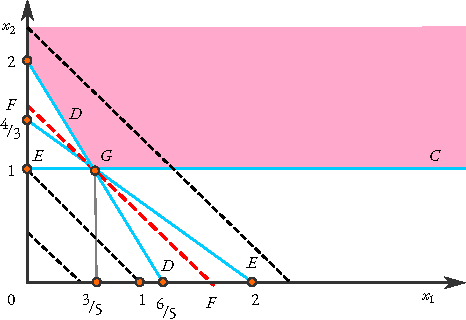
\includegraphics[width=0.85\tfwidth]{figures/aa-graph.pdf}
\caption{Solution for the game of aircrafts and anti-aircraft guns.\label{aa-graph}}
%fig 2.16
 \end{figure}

How could we use this recommendation in practice? If there is only
\redem{one} bombing raid in the ``game''. A clearly should select strategy $A_{2}$ because $p_{2} > p_{1}$. Suppose now the game has \redem{many} raids (for instance, raids on many bases). If the game is run $N$ times ($N \gg 1$), then $A$ should choose strategy $A_{1} \,\, 3N/8$ times and strategy $A_{2} \,\, 5N/8$ times.

We have so far only discussed the behaviour of $A$, allowing $B$ to act
arbitrarily. If $A$ selects his optimal mixed strategy, his average gain will
be between the upper game value of 3/4 and the game value $\nu = 5/8$. If
$B$ behaves unreasonably, the $A$'s gain may rise to the upper value of the
game (or even greater). However, if $B$ in turn adheres to his optimal
mixed strategy, the $A$'s gain will equal the game value $\nu$. The optimal
mixed strategy for $B$ precludes his use of strategy $B_{3}$ and is to use
strategy $B_{1}$ with probability 1/4 and strategy $B_{2}$ with probability 3/4.
That strategy $B_{3}$ should not be used can be seen from \figr{aa-graph}: the
straight line $EE$ corresponding to this strategy does not have any points
in the red area. To determine the probabilities with which to apply
strategies $B_{1}$  and $B_{2}$, we use the game value $\nu = 5/8$, and get $q_{1} \times 0 + (1 - q_{1}) \times 5/6 = 5/8$. It is clear from this that $q_{1} = 1/4$ and $q_{2} = 1 - q_{1} = 3/4$.

% \upsilon can be used instead of \nu

%%% Local Variables:
%%% mode: latex
%%% TeX-engine: xetex
%%% TeX-master: "twibop2"
%%% End:

% !TEX root = twibop2.tex

\chapter{Control and Self-control}
\epigraph{Cybernetics penetrated and continues to penetrate every area of man's work and daily life. This is the science of the optimal control over complex processes and systems.}  {A.I. Berg}

\section{The Problem of Control}

\txthead{Control against disorganization.} Although the world around us is full of
chance, it nonetheless proves to be organized and ordered in many
ways. \redem{The disorganizing effect of chance is countered by the organizing
influence of control and self-control.}

Suppose an airplane flies from Moscow to Leningrad. Various
random factors affect it during the flight. Therefore, all three space
coordinates of the airplane are random functions of time. The flight
trajectory is a realization of these random functions. However, these
``subtleties'' do not bother the passengers; they fasten their belts before
takeoff confident that whatever thunderstorms might occur on the way
and whichever winds affect the airplane, it will arrive at Leningrad
airport. The basis for this confidence lies in the aircraft's control system
and the actions of the pilot. We met queueing systems above, and although
there is a great deal of chance, they comply with their objectives.
This is because the organization of the system and the control of
its operation is well-designed.

\redem{Controls} take on a variety of guises. Suppose we want a set of books
to serve public for a long time. This is impeded by chances both purely
physical in nature and those related to the attitudes of some readers. So
we control matters: we take care of the binding, regulate the
temperature, humidity, and illuminance in the rooms where the books
are stored, give the book a library card, and set up the rules governing
the use of the books.

No one is safe from disease, and although each disease has a definite
cause, the prevalence and lethality of a disease on the scale, say, of
a town is governed by chance. When fighting it, we must control matters
by improving working and living conditions, taking preventive medical
measures, constructing stadiums, swimming pools, sport complexes,
ordering pharmacies to supply the necessary drugs, etc.

Thus, there is a \redem{confrontation} of two powerful factors in the world,
two basic trends. On the one hand, there is \redem{randomness}, a tendency to
disorganization, disorder, and destruction in the long run. On the other
hand, there is \redem{control} and self-control, a tendency to organization, order, development, and progress.

\txthead{Choice as a prerequisite of control.} If all the processes and
phenomena in the world were strictly predetermined, it would be
meaningless even to speak of the possibility of control. \redem{In order to
control something, there must be some choice.} How may we make
a decision if everything is predetermined in advance? Every
phenomenon must have several probable lines of development. One may
say that a world built on probability is the only world in which control
is possible.

Control acts against chance, even though the possibility of control is
brought about by the existence of chance. It is random occurrences that
help us avoid predetermination. We can say that randomness ``brings to
life'' its own ``grave-digger'', i. e. control. This is a manifestation of the
dialectic unity of the necessary and the random in the real world.

\txthead{Control and feedback.} Two different control schemes are shown in
\figr{control-scheme-1} , where $S$ is the controlled system, $CU$ is the control unit, $V$ is the input to the controlled system (the control signal), $P$ are random perturbations affecting the controlled system, and $w$ is the final output
from the system. Scheme $(b)$ differs from scheme $(a)$ in having a feedback
loop, that is the control unit receives information about the results of
control.
\begin{figure}[!ht]
 \centering
 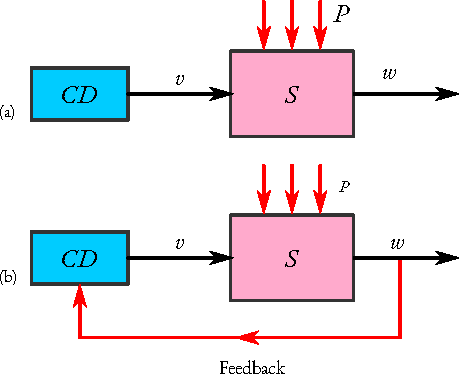
\includegraphics[width=0.75\tfwidth]{figures/control-scheme-1.pdf}
\caption{Two different control schemes.\label{control-scheme-1}}
%fig 3.1
 \end{figure}

What is feedback for? In answering this question, let me remark that
the ``relationship'' between randomness and control is one of active
confrontation. Control acts against chance, and chance acts against
control. The latter fact requires flexible control, the possibility for
adjustment. The control unit must be able continuously to receive data
about the results of the control and correct its signals to the system
appropriately.

In point of fact, any real control system supposes the presence of
a feedback loop. \redem{Control without feedback is not only ineffective, it is
actually unviable.}

Take for example someone driving a motor-car. Imagine for a minute
that the feedback suddenly disappeared, that is, the driver stopped
attending to the motion of the car. The car would continue to be
controlled, but without any feedback. The car is immediately affected by
a variety of random events. A small bump or bend in the road, a car
moving in the opposite direction all are random and could lead to an
accident in only a few seconds.

\txthead{The control algorithm.} Now what should be done and how should the system be controlled? It depends on the situation and the goal being
pursued. In fact the answer lies in the algorithm of control. 
\begin{mybox}{}
A control algorithm is a sequence of actions that must be carried out to reach a set of goals.
\end{mybox}

In the example with the car and a driver, the control algorithm
contains rules on how to start the engine, how to brake, how to turn,
how to shift gears, and so on. The algorithm also contains the traffic
regulations and good driving practice.

In some cases the control algorithm is simple. For instance, in order
to use a coffee machine, only the following two actions need be carried
out: put a coin in the slot, and press the appropriate buttons. This is the
complete control algorithm for this machine. In other cases, the control
algorithm is much more complicated. For instance, it is more difficult to
drive a car, while flying a jet is even more complicated. In very
complicated cases, the control algorithm cannot even be defined in full.
For instance, complete control algorithms for managing a large
enterprise or industry simply do not exist.

\section{From the ``Black Box'' to Cybernetics}

Despite the diversity of algorithms, the processes of control can be
investigated from general positions, irrespective of the details of the
considered system. A typical example is the simulation of a system using
the ``black box'' model.


\txthead{What is a ``black box''?} Suppose we consider a controlled system,
where $V_{1}, V_{2}, \ldots , V_{m}$ are its inputs (control signals), $P$ is a random perturbation, and $W_{1}, W_{2}, \ldots , W_{n}$ are its outputs (Figure \ref{black-box-1}). Now let us suppose that we do not know or do not care what is inside the system. We only need investigate the relationships between the inputs ( $V_{1}, V_{2}, \ldots , V_{m}$) and the outputs ($W_{1}, W_{2}, \ldots , W_{n}$). It is said in this case that the given system is a ``black box''.

\begin{figure}[!ht]
 \centering
 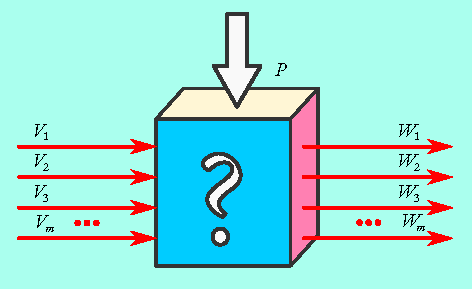
\includegraphics[width=0.8\tfwidth]{figures/black-box-1.pdf}
\caption{A black box is a system whose inputs and outputs are known, but internal structure is not.\label{black-box-1}}
% fig 3.2
 \end{figure}
 
Any controlled system is a ``black box'' if its internal structure is not
considered, and only the responses of the outputs to the inputs are
investigated.



\txthead{Man surrounded by black boxes.} The advance of science and
technology has surrounded mankind by a vast number of controlled
systems. As a rule, we are not a bit bothered by this because we quickly
get accustomed (sometimes unconsciously) to considering these systems
as black boxes. We find out how, what, and where to turn, press, or
switch the buttons to obtain the desired effect. If you want to watch
a TV show, there is no need to know the structure or workings of
a television. We need only press the proper button and select the
channel. To make a telephone call, we do not have to be telephone
engineers; we just pick up the receiver, wait for the call signal, and dial
the telephone number. We use television, telephone, and many other
systems and consider them to be black boxes. Naturally, we could learn
what is inside the system and how it works if we want to, but in our
modern world we often think it's a waste of time to study what we can
quite do without in practice. More and more often we prefer to use
black boxes and when they fail we call in a professional technician.

We should recognize the validity of the complaints that as modern
people we have become less curious, that we do not want to see things
in depth because there are too many things to see, and it is not difficult
to use them. However, I should not make things appear to be worse
than they are. Firstly, there is a system of universal secondary education
at least in the developed countries, which ensures each person has
a basic minimum knowledge. Secondly, from the viewpoint of the
development of society, the knowledge available to the society
as a whole is more important than what a single person may
know.

\txthead{Complex systems as black boxes.} Modern systems are becoming more
and more sophisticated as their functional capacities become more and
more diverse. Naturally, the more we need to know about the functions
of a system, the further we push our investigation of its inner structure
into the background, and in many cases such a total investigation would
prove infeasible because of the complexity of the system.

This shift of emphasis leads us to a qualitatively new viewpoint, in
which the main aim is to investigate control and self-control as general
processes irrespective of the concrete devices comprising the systems.
This point of view brings about \redem{cybernetics} as the science of control
(self-control) in complex systems.

Curiously this point of view reveals an interesting fact and makes us
look at the black-box model in another way. It turns out that we do not
need understand every structural subtlety of a complex system, indeed
its separation into component parts can obscure essential information.
The black-box model becomes \redem{fundamental} as the only acceptable way
of analyzing a complex system.

\txthead{What is cybernetics?} The science of cybernetics was founded by the American scientist Norbert Wiener (1894-1964) and dates from 1948
when he published his famous book \redem{Cybernetics, or Control and
Communication in the Animal and the Machine}. Wiener wrote:
\begin{quote}
``We have decided to call the entire field of control and
communication theory, whether in the machine or in the animal, by the
name cybernetics, which we form from the Greek $\varkappa \upsilon \beta \epsilon \rho \nu  \eta \tau \eta \zeta$, or steersman.''\\[-10pt]
\end{quote}
It should be noted that the term ``cybernetics'' was not new. Plato
used it meaning the art of controlling ships. The French physicist
Amp\'ere classified sciences in the first half of the $19^{\text{th}}$ century and placed a science, which was the study of the methods of government, in section
83. Amp\'ere called this science cybernetics. Today we only use the term
``cybernetics'' in the sense given to it by Wiener. 
\begin{mybox}{}
Cybernetics is the science of the control and communication in complex systems, be they machines or living organisms.
\end{mybox}

The Soviet scientist L.A. Rastrigin wrote a book called \redem{This Chancy,
Chancy, Chancy World} (Mir Publishers, Moscow, 1984), in which he
remarked:
\begin{quote}
``Until cybernetics made its appearance, control processes in an
electric generator were investigated by electrical engineering, control of
the motion of a clock pendulum (in effect a swing) was dealt with in
mechanics, and control of population dynamics in biology. Norbert
Wiener was the first to point to the universal nature of control and to
show that the organizing of an object (the lowering of its entropy) could
be achieved by means of standard procedures, that is, by applying the
methods of cybernetics independently of the physical characteristics of
the object."
\end{quote}
L.A. Rastrigin imaginatively calls cybernetics a science which fights
randomness, thus emphasizing the idea of control counteracting
disorganization and destruction caused by diverse random factors.

\txthead{Cybernetics and robots.} One of the central topics of cybernetics
concerns \redem{process automation}, in particular, \redem{self-control in complex systems}. Investigations into this area resulted in the appearance of a discipline called ``robotics''. Modern cybernetics literature discusses the possibility of designing automata that can reproduce and teach themselves.
Artificial intelligence is also a topic being investigated. The following
questions are being studied: Is the machine capable of creativity? Could
a machine become cleverer than its designer? Could the machine think?

The more sophisticated types of robots are still in the realms of
science fiction, although we often hear discussions about the possibilities
of robotics, or rather whether artificial ``men'' might be possible. The
layman now seems to believe that cybernetics is indeed simply the
science of robots, automata, or thinking machines. The true purpose of
cybernetics as the science of control is now masked by the fantastic
technological promise.

True, cybernetics does include the problems of automation, and thus
contributes to scientific and technological progress. The automation of
various processes, the design of automatic Lunar explorers, automatic
space docking are all achievements of cybernetics. Cybernetics also
investigates computer creativity and artificial intelligence. However, this
is not so as to evolve an artificial person. When we programme
computers to ``compose'' music or ``write'' a poem or play chess or give
a ``talk'', we are attempting to simulate creativity and so find out more
about these processes. It could be said that we are investigating the limit
of computer abilities, but not that we want to substitute them for
human beings in the future: we just want to understand several
important topics thus making it possible to go deeper into the control
processes occurring in human beings. The reader should remember this
and not consider cybernetics to be just the ``science of robots''.

We may now start discussing the central notion of cybernetics, i. e.
\redem{information}. Let me say right away that cybernetics investigates control
and self-control primarily from the viewpoint of information. It
investigates the collection, conversion, transmission, storage, and
retrieval of information. In a certain sense of the word, cybernetics can
be regarded as the ``science of information''.

\section{Information }

Let me begin with an excerpt from the immortal poem \redem{De Rerum
Natura} (On the Nature of Things) by Carus Lucretius (ca. 99-55 B.C.):
\begin{quote}
`` \ldots if things came to being from nothing,\\
Every kind might be born from all things,\\
Nought would need a seed.\\
First men might arise from the sea, and from the land,\\
The race of scale creatures, and birds burst forth \\
The sky. Cattle and other herds, and all the tribe\\
Of wild beasts with no law of birth,\\
Would haunt tilth and desert \ldots ''
\end{quote}
It is interesting that there is here a hint of the conservation of not
only matter and energy, but also of something else, which is neither
matter nor energy. There is no shortage of energy and matter in the sea,
but people do not appear in the sea. Nor too does the dry land produce
fish. Truly, ``if things came to being from nothing, \ldots{} nought would need
a seed''. In the modern terminology of science, we might say that this is
a hint of the \redem{conservation of information}. The information needed by
plants and animals to live and reproduce cannot appear ``from nothing''.
It is stored in ``seeds'' and thus handed down from generation to
generation.

The term ``information'' is now encountered everywhere in science and
everyday life. In fact, every activity is related to the \redem{collection,
conversion, transmission, storage, and retrieval of information}. We live in
a world filled with information, and our very existence is impossible
without it. Academician A.I. Berg once said: ``Information penetrates
every pore of the life of human beings and their societies \ldots{} Life is
impossible in a vacuum of either mass-energy or information.''


\txthead{The bit, the unit of information.} What is information? What units is it
measured in? Let us start with a simple example. A train approaches
a station. By remote control, a signalman can switch a train from one
track $(A)$ to another $(B)$. If the switch is up, the train goes along track $A$, and if it is down, the train goes along track $B$. Thus, the signalman, by
moving the switch up or down, is sending a control signal containing
1 bit of information. The word ``bit'' is an abbreviation of ``binary digit''.

To see what we mean by ``binary digit'', recall how digits are used to
write numbers. We commonly use the decimal number system, i.e.
a system with ten digits (0, 1, 2, \ldots , 9). Take a number written in the
\redem{decimal} system, say 235. We say ``two hundred and thirty five'' and, as
a rule, do not pause to think that this means the sum of two hundreds,
three tens, and five units, i. e. $2 \times 10^{2} + 3 \times 10 + 5 \times 10^{0}$. The same number (235) can also be in the \redem{binary} system, which only has two digits, 0 and 1, as 11101011, which means $1 \times 2^{7} + 1 \times 2^{6} + 1 \times 2^{5} + 0 times 2^{4} + 1 \times 2^{3} + 0 \times 2^{2} + 1 \times 2^{1} + 1 times 2^{0}$. Since $2^{7} = 128, \, 2^{6} = 64, \, 2^{5} = 32, \, 2^{3} = 8, 2^{1} = 2, \,\, \text{and} \,\, 2^{0} = 1$, we have our number $128 + 64 + 32 + 8 + 2 + 1 = 235$. Any number can be written in either the
decimal or the binary system. If you don't follow this explanation try
looking at \figr{binary-conversion}.

\begin{figure}[!ht]
 \centering
 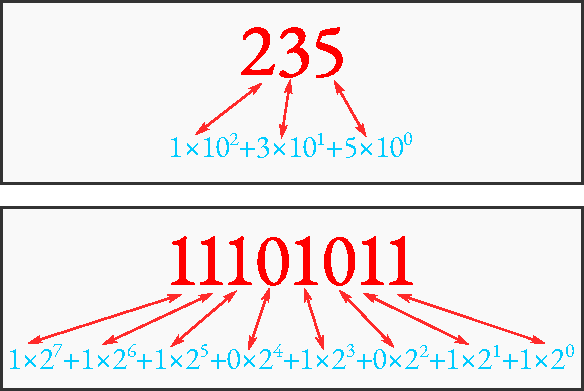
\includegraphics[width=0.75\tfwidth]{figures/binary-conversion.pdf}
\caption{Representing the number 235 in decimal and binary systems.
\label{binary-conversion}}
% fig 3.3
 \end{figure}

Let us return to the railway example. Remember we have two choices:
the switch is either up (track $A$) or down (track $B$). We could write the
digit 0 for switch up and digit 1 for switch down. It can be said that the
control signal can thus be coded by one of the two binary digits, zero or
unity. The signal thus contains one binary digit, or 1 bit of information.

Consider a more interesting example. The railway lines near a station
are shown in \figr{railway-switches}. 

\begin{figure}[!ht]
 \centering
 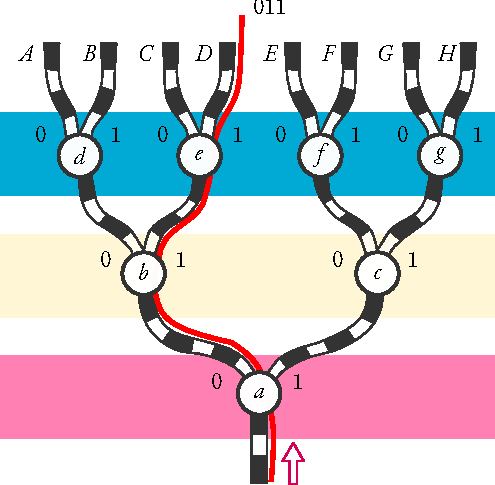
\includegraphics[width=0.8\tfwidth]{figures/railway-switches.pdf}
\caption{Controlling railway lines by using switches.\label{railway-switches}}
% fig 3.4
 \end{figure}

The railway switches are labelled by the letters $a, \,
b, \, c, \, d, \, e, \, f$, and $g$. If a switch receives a control signal of 0, it opens the left-hand track, and if it receives a signal of 1, it opens the right-hand
track. The signalman has three control switches: the first one sends
a signal (0 or 1) to railway switch $a$, the second one sends a signal
simultaneously to switches $b$ and $c$, and the third one simultaneously to
switches $d, \, e, \, f,$ and $g$. The station has eight tracks: $A, B, C, D, E, F, G,$ and $H$. To send a train along track $A$, all three control switches must be turned to the 0 position, i.e. send the three-digit signal 000. To direct
a train to track $B$, it is necessary to send the three-digit signal 001. Each
track thus has its own three-digit signal, i.e.
\begin{center}
\setlength\arrayrulewidth{0.75pt}\arrayrulecolor{Tomato}
\begin{tabular}{cccccccc}
\toprule
A & B & C & D & E & F & G & H\\
\midrule
000 & 001 & 010 & 011 & 100 & 101 & 110 & 111 \\
\bottomrule
\end{tabular}
\end{center}

We see that to select one of the eight outcomes requires a set of
elementary signals, each of which carries 1 bit of information. Therefore,
to choose a track in this example requires three bits of information.

Thus, in order to select one option out of two, 1 bit of information is
required; in order to select one option out of eight, 3 bits of information
are required. In order to select one of $N$ options, $I$ bits of information
are required, where
\begin{equation}%
I = \log_{2} N.
\label{eq-3.1}
\end{equation}
This is the \redem{Hartley formula}. It was suggested in engineer Ralph Hartley, who was interested information.

\txthead{The Bar Kohba game.} A rebellion against Romans broke in 135 A. D.
in the ancient Judea led by one Bar Kohba. As the legend has it, Bar
Kohba sent a spy into the camp of Romans, and the spy discovered
a great deal before being caught. He was tortured and his tongue was
cut out. However, the spy managed to escape, but without his tongue he
could not report what he had found out in the enemy's camp. Bar
Kohba resolved the problem by asking the spy questions that only
required a ``yes'' or `no'' answer (it was only necessary to nod or shake
the head). Bar Kohba was able to obtain all the information he wanted
from his spy, even though the spy had no tongue.

A similar situation is described in \redem{Le comte de Monte Christo} by
Alexandre Dumas p\'ere. An old man in the novel had been paralyzed
and could neither speak nor move his hands. Nonetheless, his relatives
were able to communicate with him asking him questions which
required only a ``yes'' or a ``no''. If ``yes'', the old man would close his
eyes; if he blinked several times, it was ``no''.


It turns out that any information can be transmitted in the form of
``yes'' and ``no'' answers if the questions are constructed \redem{properly}. This idea underlies the \redem{Bar Kohba game}, which first appeared at the turn of the century in Hungary and then spread to other countries. A player
thinks of something. He may, for instance, make a wish or even think
up a sentence. The other player must guess the wish or sentence by
asking questions, which must be honestly answered. However, the
questions may only require a ``yes'' or ``no'' answer. The quantity of
information needed for a correct guess can be measured by the number
of questions, given that the most rational method of interrogation is
used. Each answer can be enciphered by a binary digit, for instance, we
could use a one for a ``yes'' and a zero for a ``no''. Then the information
needed for a correct guess would be a combination of zeroes and unities.

Let us play a Bar Kohba game with the railway signalman at the
station whose tracks are given in \figr{railway-switches}. The signalman thinks of a track along which a train should travel to the station. We want to
guess the track. The game would go as follows.
\begin{dialogue}
\ques Should switch $a$ open the track on the right?
\ans No. (let us cipher this answer by digit 0).
\ques Should switch $b$ open the track on the right?
\ans Yes (we cipher: 1). 
\ques Should switch $e$ open the track on the right? 
\ans Yes (we cipher: 1).
\end{dialogue}
Having asked these three questions, we see that the signalman decided
on track $D$. The information needed to answer was the chain of answers
``no-yes-yes'' or, in other words, by the set of binary digits 011. We
know that the information capacity of the signalman's ``riddle'' was three
bits long. Each of the signalman's three answers contained one bit of
information.

Let me cite one more example of the Bar Kohba game. There are 32
pupils in a class. The teacher decides on one of them. How can we find
out which one? Let us take the class register, in which the surnames of
all the pupils are listed in alphabetical order and enumerated. Let us
start asking questions.
\begin{dialogue}
\ques Is the pupil among those listed from 17 to 32? 
\ans Yes (we cipher: 1).
\ques Is the child among those listed from 25 to 32?
\ans No (0). 
\ques Is the child among those listed from 21 to 24?
\ans No (0). 
\ques Is the child among those listed either 19 or 20?
\ans Yes (1).
\ques Is it number 20?
\ans No (0).
\end{dialogue}
Consequently, the teacher meant pupil number 19 in the class register.
This information required the chain of answers ``yes-no-no-yes-no'' or, in
other words, the set of binary digits 10010. It is clear from \figr{32-pupils} that the area in which the surname was searched for gradually decreased
with each answer. To solve the problem, it only required to ask five
questions. According to the Hartley formula, the selection of the option
out of 32 requires log, $3^{2} = 5$ bits of information. Therefore, each of the
answers in this game contained 1 bit of information.
\begin{figure}[!ht]
 \centering
 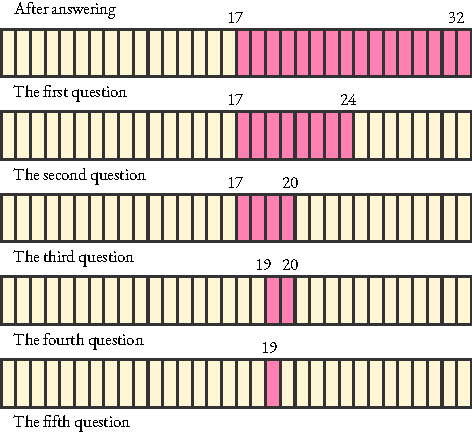
\includegraphics[width=0.85\tfwidth]{figures/32-pupils.pdf}
\caption{Finding out the selected pupil from a group of 32.\label{32-pupils}}
% fig 3.5
 \end{figure}

Perhaps I have created the impression that each answer in the Bar
Kohba game always contains 1 bit of information. It is easy to see that
this is not so. Suppose that we established that a surname was listed
from 17 to 32 and then ask: Is it the surname listed from 9 to 16? It is
dear that the answer to this question must be negative. The fact that the
answer is obvious means that it does not contain any information at all.
Naturally, we might have a situation without ``silly'' questions.
\begin{dialogue}
\ques Is the surname listed from 1 to 8?
\ans No.
\ques Is it listed from 25 to 32?
\ans No.
\ques Is it listed from 9 to 16?
\ans No.
\ques Is it listed from 17 to 24?
\ans Yes.
\ques Is it listed either 23 or 24?
\ans No.
\ques Is it listed either 19 or 20?
\ans Yes.
\ques Is it listed 19?
\ans Yes.
\end{dialogue}
Having chosen this strategy, we extracted the needed information
using eight questions rather than five. The quantity of information in the
final answer equals 5 bits as before. Therefore, each individual answer in
this case contained, on the average, 5/8 bit of information.

Thus, we see that ``yes-no'' answers do not always contain 1 bit of
information. Running ahead of ourselves, we can note that 1 bit is the
\redem{maximum} information that such an answer may contain.

``Just a minute,'' you might say, ``if this is so, does then a binary digit
not always carry one bit of information?''

``Quite true,'' I would answer.

``Then how about the definition of a bit of information given above?
Can we use the Hartley formula?''

All that has been said about a bit of information (and about the
Hartley formula) remains valid, although with a reservation that \redem{every
option should be equally probable}. I did not want to discuss this topic too
early, but now the time has come to do so.

\txthead{Information and probability. The Shannon formula.} I have
emphasized that control is only possible in a world where necessity is
dialectically confronted with chance. In order to control something,
there must be choice. Any situation we want to control carries with it
uncertainty. This uncertainty can be compared with a shortage of
information. While we control an object, we introduce information and
thus decrease the uncertainty.

For instance, a train may arrive along any of the eight tracks in our
example above, so there is uncertainty. By sending a control signal with
three bits of information, the signalman eliminates this uncertainty, and
the train is directed along one particular track. The teacher could have
thought of any of his 32 pupils, so there was uncertainty which surname
had been chosen. Having listened to the answers for a number of
questions with an overall quantity of information of five bits, we can
eliminate this uncertainty and identify the pupil.

Now let us return to the starting point of our reasoning and to the
presence of choice. Until now, we assumed that each option was equally
probable. The signalman could have chosen any of the eight tracks with
equal probability. The teacher could have picked anyone of his 32
pupils. However, we often have to choose between options that are not
equally probable, and then it is necessary to pay due attention to the
\redem{probability associated with each option}. Suppose the answer to a question may be either ``yes'' or ``no'' and both outcomes are equally probable.
The answer then will carry precisely 1 bit of information. However, if
the ``yes'' or ``no'' outcomes have different probabilities, then the answer
will contain less than 1 bit of information. And the greater the difference
between the probabilities of the two outcomes, the smaller the quantity
of information. In the limit of the probability of a ``yes'' (or a ``no'')
being unity, the answer will not contain any information at all.

Now, let us look at what happens when different outcomes (different
options) have different probabilities. I do not want to cram this book
with mathematics, so I shall only discuss the basic results. Suppose $\xi$ is
a random discrete variable that may assume the values $x_{1}, x_{2}, x_{3},\ldots{} , x_{N}$ with probabilities  $p_{1}, p_{2}, p_{3},\ldots{} , p_{N}$, respectively. We have $N$ outcomes ($N$ different values of the random variable) which appear with different probabilities. Given an observation of the variable $\xi$ and its value, how much information does this observation carry?

This problem was investigated by the American scientist Claude
Shannon in the mid-1940s. He came to the conclusion that we obtain
the quantity of information equal (in bits) to
\begin{equation}%
I(\xi) = \sum_{i=1}^{N} p_{i}  \log_{2} \frac{1}{p_{i}}.
\label{eq-3.2}
\end{equation}
This is a fundamental relation in information theory. It is called the
\redem{Shannon formula}.

Suppose that the outcomes are equally probable, and the random
variable may take on the values $x_{i}$ with the same probability $p$. This
probability is clearly $1/N$ and so from \eqref{eq-3.2} we obtain
\begin{equation*}%
I =  \frac{1}{N} \, \sum_{i=1}^{N}   \log_{2} \, N = \frac{1}{N} \, N \,  \log_{2} N =   \log_{2} \, N,
%\label{shannon-formula}
% eq 3.2
\end{equation*}
i.e. the Hartley formula \eqref{eq-3.1}. Consequently, we see that the Hartley formula is a special case of the Shannon formula when all outcomes are
equally probable.

Using the Shannon formula, let us find how much information can be
contained in a ``yes'' or ``no'' answer. Suppose $p$ is the probability of
a ``yes''. Then the probability of a ``no'' answer is $1 - p$. According to
\eqref{eq-3.2}, the information obtained from the answer to a question is
\begin{equation}%
I = p \ \log_{2}  \frac{1}{p} + (1 - p)   \log_{2} \frac{1}{1-p}.
\label{eq-3.3}
% eq 3.3
\end{equation}
The graph of $I$ versus $p$, as defined by \eqref{eq-3.3}, is given in \figr{shannon-distro}.


Maximum information (1 bit) is obtained when $p = 1/2$, i.e. when
a ``yes'' and a ``no'' are equally probable. Now we can refine our notion
of ``1 bit of information''. \redem{This is the information contained in a digit that may take on only two values provided both values are equally probable}.

It follows that the best strategy in the Bar Kohba game is to ask
``yes'' or ``no'' questions, the answers to which are nearly or equally
probable. Recall the question: ``Is the surname listed from 17 to 32?''
Here the answers ``yes'' and ``no'' are equally probable because there are
32 pupils and the numbers from 17 to 32 cover half of the pupils. Therefore,
the answer to this question gives 1 bit of information. But for the
question: ``Is the surname listed from 1 to 8?'' the range of numbers
only covers a quarter of all the numbers and therefore the probability of
a ``yes'' is 1/4, while that of a ``no'' is 3/4. The answer to this question
would contain less than 1 bit of information. According to \eqref{eq-3.3}, in which we substitute $P = 1/4$, each answer contains 0.8 bit of information.


\begin{wrapfigure}{O}{\mfwidth}
 \centering
 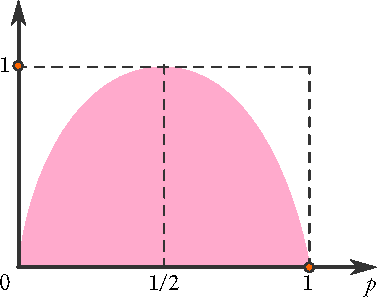
\includegraphics[width=\linewidth]{figures/shannon-distro.pdf}
\caption{Graph of Shannon distribution.\label{shannon-distro}}
 \end{wrapfigure}


Once again I emphasize that control processes should be regarded in
a dialectical unity with the random processes of disorganization. There
is a deep relationship between information theory and probability
theory. The Shannon formula \eqref{eq-3.2} illustrates this point. The
probabilistic approach provides a scientific, objective notion of
information that is free from a subjective substitution of the quantity of
information by its significance or importance.



\txthead{Information in communication channels with noise.} When information is transmitted, some loss is unavoidable. This happens because of the action of random factors, which are commonly lumped together as noise. A \redem{communication channel} for transmitting information from input set $A$ to output set $B$ is represented in \figr{comm-channel}. The information is affected by noise $P$ as it is transmitted. Suppose that $\xi$ is an input discrete random variable which may assume values $x_{1}, x_{2}, x_{3},\ldots{} , x_{N}$. with probabilities  $p_{1}, p_{2}, p_{3},\ldots{} , p_{N}$, and $\eta$ is the output variable, which may assume values $y_{1}, y_{2}, y_{3},\ldots , y_{M}$. with probabilities  $q_{1}, q_{2}, q_{3},\ldots{} , q_{M}$. Let $P_{i}(j)$ denote the probability that $\xi = y_{j}$ is the output variable if $\xi = x_{i}$ was transmitted. The probability $P_{i}(j)$ is determined by noise in the communication channel. It has been proved in information theory that the quantity of information about the random variable $\xi$ that can be obtained by observing the random variable $\eta$ is described by the formula
\begin{equation}%
I_{\eta} \, (\xi) = \sum_{i=1}^{N}\sum_{j=1}^{M} P_{i}(j) \, p_{i}  \, \log_{2} \frac{P_{i}(j)}{q_{i}}.
\label{eq-3.4}
% eq 3.4
\end{equation}
\begin{figure}[!ht]
 \centering
 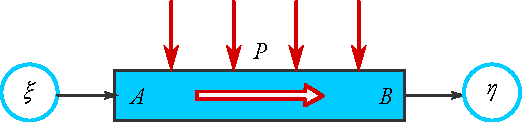
\includegraphics[width=0.8\tfwidth]{figures/comm-channel.pdf}
\caption{A communication channel for transmitting information.\label{comm-channel}}
% fig 3.7
\end{figure}
Here the information $I$ is in terms of two types of probability, the
probabilities $p_{i}$ and $q_{j}$ on the one hand and the probability $P_{i}(j)$ on the other. While the first two probabilities reflect the probabilistic nature of
the information at the input of the communication channel and that
``yes'' or ``no'' questions, the answers to which are nearly or equally
probable. Recall the question: ``Is the surname listed from 17 to 32?''
received at the output, probability $P_{i}(j)$ reflects the random nature of
the noise in the channel.

Suppose there is no noise. Then the random variable values at the
input and the output of the channel will be the same. Hence
\begin{equation}%
N = M, \,\, p_{i}= q_{i}, \,\, \text{and} \,\, P_{i}(j) = \delta_{ij},
\label{eq-3.5}
%eq 3.5
\end{equation}
where $\delta_{ij}=1$ for $i = j$ and $\delta_{ij} = 0$ for $i =1= j$.
Substituting \eqref{eq-3.5} into \eqref{eq-3.4} and noting that $\lim\limits_{z \to 0} z \, \log_{2} \, z = 0$, we get the Shannon formula. This should have been expected because when there is no noise, there is no loss of information in its transmission.


\txthead{Protection against noise in a communication channel.} There are many
sorts of communication channel. Information can be transmitted by
sound waves propagating in a medium, electric signals running along
wires, electromagnetic waves propagating in a medium or in vacuum,
etc. Each communication channel is affected by its own sorts of noise.
There are general techniques for handling noise that can be applied to
any communication channel. First of all, it is desirable to minimize the
level of noise and maximize the amount of information in the signals, so
that the signal-to-noise ratio is large. The ratio can be increased by
coding the transmitted information appropriately, e. g. transmitting it in
terms of ``symbols'' (for instance, impulses of a certain shape) which can
be distinctly identified against the background of noise. Coding a signal
increases its ``noise immunity'' or performance in terms of error
probability for the transmission.
\begin{figure}[!ht]
 \centering
 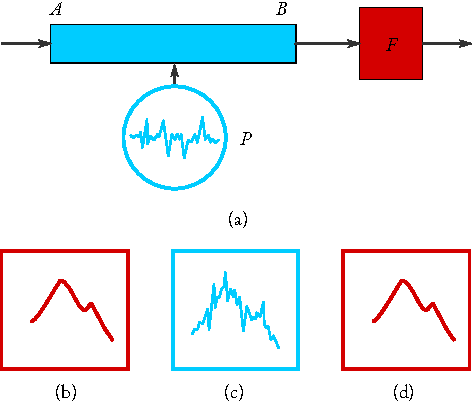
\includegraphics[width=0.8\tfwidth]{figures/noise1.pdf}
\caption{A communication channel with a filter.\label{noise1}}
% fig 3.8
 \end{figure}
 
A special measure against noise is \redem{filtering} (both \redem{smoothing} and
\redem{correlation}) the information received at the output of communication
channels. If the characteristic noise frequency in a communication
channel is substantially greater than the frequency typical for the time
change in the signal, we could use a \redem{smoothing filter} at its output to ``cut out'' the high-frequency oscillations superimposed on the signal as it was
transmitted. This is illustrated in \figr{noise1}, in which (a) is a diagram of the communication channel with a filter ($A$ is the channel input, $B$ is the
channel output, $P$ is noise, and $F$ is a smoothing filter), (b) is the signal at the input, (c) is the signal at the output before filtering, and (d) is the signal after filtering.
\begin{figure}[!ht]
 \centering
 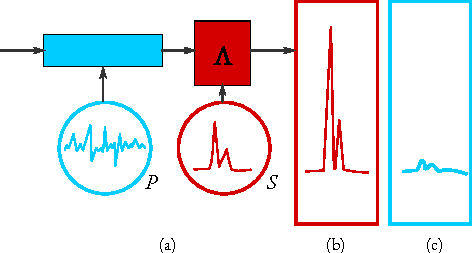
\includegraphics[width=0.8\tfwidth]{figures/noise2.pdf}
\caption{A communication channel with a filter and signal multiplier.\label{noise2}}
% fig 3.9
 \end{figure}
 
Suppose we want to find out whether the output contains a signal of
a given shape. If the signal is very different (for instance, by frequency)
from the noise background, it will be easily identified. The situation is
worse when the signal is ``masked'' by noise. Correlation filtering is
applied in these cases: a device is placed at the output which \redem{multiplies}
the output signal by the known signal. If the desired signal is present in
the output signal, the multiplication creates a very clear (large) final
(correlation) signal; otherwise no correlation signal will appear. This is
illustrated in Figure \ref{noise2}, in which (a) is a diagram of the channel ($\Lambda$ is the signal multiplier, $P$ is noise, and $S$ is the signal shape to be recognized), (b) is the multiplied signal if the recognized signal $S$ is present in the output (the correlation signal), and (c) is the multiplied signal if signal $S$ is absent in the output. Correlation filtering is used, for instance, in radar scanners to recognize the radiation signal emitted by the radar antenna.

%\clearpage

\section{Selection of Information from Noise}

\txthead{Where does information come from and some unsatisfactory answers.} Any control signal carries certain information. The signal is formed
using an algorithm which itself incorporates information, and this
algorithm was compiled in turn using information contained in other
algorithms. Thus we have a sort of relay race in which information is
transmitted from algorithm to algorithm. This idea can be illustrated by
a simple example. A teacher educates you, and in turn your teacher had
a teacher, who had a teacher, and so on.

This argument leads inevitably to the questions: Whence the ``original
information''? Whence the first algorithm? An inability (or reluctance)
to investigate scientifically the fundamental topic of where information
comes from leads to serious misconceptions.

One such misguided hypothesis is that the original information was
brought to the Earth by space travellers, who visited us in some
long-forgotten past. This hypothesis is materialistic, but it is unsatisfactory
because it begs the question of where the aliens got the
information. Modern science indicates where the information comes
from. The modern scientific answer is that there is no ``original
information'': the generation of information is a continuous and
continuing process.

\txthead{Chance at the forefront again.} The idea of information being handed
over like a relay baton in a race is simplistic. I pointed out that any
transmission of information is accompanied by loss caused by random
factors. However, random factors not only ``steal'' information, they also
generate it.

At first glance, this seems implausible. We witness the continuous
creation of information as a result of human creativity. New machines
are designed, spacecraft are launched, new books are published, and new
drugs become available: these are all a testimony to the explosive
generation of information in which everybody participates. So it would
seem strange to speak of the fundamental role of chance in generating
information.

However, consider the \redem{process of thinking}, how a problem is solved,
how an intuition appears, or how a melody or image emerges. If these
examples are too philosophical, try and think at least about \redem{associative
perception}, that is how we recognize objects and distinguish them. Just
try, and you will step into a domain of complicated links, probabilistic
relationships, chance guesses, and sudden ``revelations''. There are no
deterministic algorithms for making discoveries or solving problems.
Everything we know about the processes occurring in the brain indicates
the \redem{fundamental role} of random factors. Later I shall illustrate this by the example of \redem{perceptron}, a cybernetic device which can recognize patterns.

\txthead{Chance and selection.} How can chance generate information? How
can order appear from disorder? It turns out that the generation of
information from noise can be easily observed. You can see this for
yourself using the game of scrabble, or rather the small lettered blocks.
Put one block with each letter of the alphabet into a bag, mix them, and
take one out at random. Write down each randomly taken letter and
return the block to the bag. Each time shake the bag. This simple
generator of random letters can be used to generate a long chaotic
string. If you look closely, you will find some three-letter words, perhaps
even words with more letters. Information is being generated from noise.

My son, for example, helped me do an experiment and in a string of
300 random letters found nine three-letter words and two four-letter.
This argument leads inevitably to the questions: Whence the ``original
information''? Whence the first algorithm? An inability (or reluctance)
words. The more letters there are in a word, the smaller the probability
of generating the word from ``letter noise''. The generation of a sentence,
let alone a line from a well-known work, is less probable. Nonetheless,
the probability of doing is nonzero, and so there is the possibility of any
information being generated randomly from noise.

Thus, we can say (although this sounds strange) that \redem{chance generates
information by chance}. The greater the information, the smaller the
probability of its random generation. That random information can be
generated does not solve the basic problem. This randomly generated
information must be detected from the enormous flow of meaningless
``signals''. In other words, the \redem{information must be selected from the noise}. In the example of taking lettered blocks out, the information is selected
from the noise by the person who wrote out the letters and looked
through the string.

\txthead{Selection amplifier} Is it possible to use chance conscientiously to
generate information? It is, so long as we \redem{amplify the selection}.

You can do a simple experiment to demonstrate the amplification of
selection using the random letter generator described above. In order to
amplify the selection, we take into account the frequency with which
letters appear in each word. Letter frequencies in English are often given
when you buy a commercial game of scrabble. To allow for the frequencies,
first eliminate the rare letters, e. g. $Z, Q, J, V, X$ and add extra
blocks with frequent letters, e. g. four blocks with $E$ and $T$, three with $A,
I, O, L, N, G, R, S$, two with $D, U,$ and one of all the rest. I cannot
vouch that this selection is optimal, in a similar experiment I found 21
three-letter words, 4 four-letter words and 1 five-letter word in
a succession of 300 random letters.

In order to amplify the selection still greater, we should use \redem{words}
rather than \redem{letters}. It is curious that a similar device was suggested in
the early $18^{\text{th}}$ century by the English satirist Jonathan Swift in
Gulliver's travels. When Gulliver visited the Academy in Lagado (the
capital of an imaginary kingdom), he met a professor who had an
interesting apparatus. Swift wrote:
\begin{quote}
``He then led me to the frame, about the sides whereof all his pupils
stood in ranks. It was twenty feet square, placed in the middle of the
room. The super faces were composed of several bits of wood, about the
bigness of a die, but some larger than others. They were all linked together
by slender wires. These bits of wood were covered on every square
with papers pasted on them, and on these papers were written all the
words of their language in their several moods, tenses, and declensions,
but without any order. The professor then desired me to observe, for he
was going to set his engine at work. The pupils at his command took,
each of them, hold of an iron handle, there were forty fixed around the
edges of the frame, and given then a sudden turn, the whole disposition
of the word was entirely changed. He then commanded six and thirty of
the lads to read the several lines softly as they appeared on the frame;
and where they found three or four words together they might make part of a sentence, they dictated to the four remaining boys who were scribes. This work was repeated three or four times, and at every turn the engine was so contrived, that the words shifted into new places, as the square bits of wood moved upside down.''
\end{quote}
True, Swift wrote satirically, laughing about such inventions.
However, why should we not believe that a talented popular-science
writer disguised himself behind mask of a satirist so as not to be
laughed at and misunderstood by his contemporaries?

What seemed absurd and laughable in the $18^{\text{th}}$ century has now
become the subject of scientific investigation in the mid-$20^{\text{th}}$ century. The English scientist W. Ross Ashby suggested a cybernetics device in
the early 1950s which could be a \redem{selection amplifier}. Ashby called it an
\redem{intelligence amplifier}. A diagram of this amplifier is given in \figr{selection-amp}.

\begin{wrapfigure}{O}{\mfwidth}
 \centering
 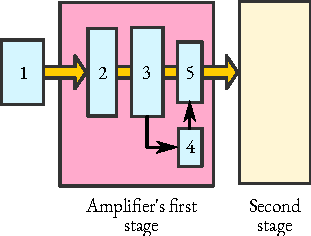
\includegraphics[width=\linewidth]{figures/selection-amp.pdf}
 \caption{A selection amplifier.\label{selection-amp}}
% fig 3.10
 \end{wrapfigure}
Noise generator 1 supplies ``raw material'' to the first stage of the
amplifier. The noise converter 2 produces various random variants of
the subjects to be selected. The selection is performed in unit 3 in
compliance with criteria of selection put into this device. In a concrete
case, if the result of a selection meets a criterion, control unit 4 opens
valve 5 and lets the selected information into the converter of the next
stage of the amplifier. One can easily imagine that the first stage of the
amplifier, supplied with random letters, selects separate randomly
emerging words or separate typical syllables; the second stage of the
amplifier selects word combinations; the third stage selects sentences,
the fourth stage selects ideas, etc.

\txthead{Random search-related self-organization. The homeostat.} Suppose
a system is in a state which a allows it to carry out certain functions. Let
us call this state \redem{normal}. It corresponds to external. conditions in which
the system operates. Suppose these conditions change all of a sudden,
and the result is that the system departs from the normal state. The new
conditions correspond to a new normal state. It is desirable to transfer
and where they found three or four words together they might make
part of a sentence, they dictated to the four remaining boys who were
scribes. This work was repeated three or four times, and at every turn
the system to this new state. How is it to be done? Information is
needed firstly on the new state, and, secondly, on how the transition of
the system to the new state can be carried out. Since the change in the
environment is random in nature, we know neither the new normal state
nor how to organize a transition to it. A \redem{random search} may help in
such situations. This means that we should randomly change the
system's parameters until it randomly matches the new normal state,
which can be immediately recognized by monitoring the system's
behaviour.

\begin{wrapfigure}[15]{O}{\mfwidth}
 \centering
 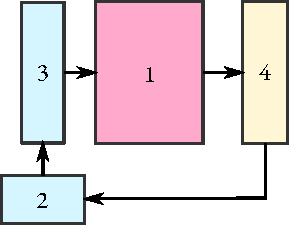
\includegraphics[width=0.9\linewidth]{figures/homeostat.pdf}
\caption{A homeostat is a device which possessed the property of
self-organization on the basis of random search.\label{homeostat}}
% fig 3.11
 \end{wrapfigure}

It can be said that the process of random search generates the
information needed to transfer the system to the new normal state. This
is nothing else but the \redem{selection of information from noise} about which we have been talking. The selection criterion here is the change in the
system's behaviour: once in the new normal state, the system ``calms
down'' and starts functioning normally.

In 1948 Ashby designed a device which possessed the property of
self-organization on the basis of random search. He called the device
a \redem{homeostat}. A diagram of a homeostat is shown in \figr{homeostat}.

A homeostat is often compared to a sleeping cat. If the cat is bothered,
it wakes up, chooses a new more comfortable position, and goes to sleep
again. A homeostat behaves in a similar manner: when it is ``woken up'',
it carries out random search for new values for its parameters, and when
it finds them, it ``goes to sleep'' again.

\begin{wrapfigure}[20]{O}{\mfwidth}
 \centering
 
\includegraphics[width=0.9\linewidth]{figures/fonts.pdf}
\caption{A selection of different ways of writing letter A.}
\label{fonts}
% fig 3.12
 \end{wrapfigure}

System 1 in \figr{homeostat} may be either in a stable or unstable state.
Without going into detail, let me note that system 1 consists of four
electromagnets whose cores can move and control the rheostats which
control the voltages across the electromagnets. Therefore, the rotation
angle of each electromagnet is dependent on all the other ones. These
angles are the parameters of this dynamic system. The magnet cores do
not rotate when the system is in a stable state. However, if an external
disturbance takes the system out of its stable state, control unit
2 switches on generator 3 of random changes of parameters, and the
random search starts. Once system 1 finds a stable state (by chance),
the system to this new state. How is it to be done? Information is
needed firstly on the new state, and, secondly, on how the transition of
the system to the new state can he carried out. Since the chance in the
unit 4 having verified the stability sends a signal to control unit 2, which
switches off the random parameter generator 3.

\section{On the Way to a Stochastic Model of the Brain}

\txthead{The pattern recognition problem.} We do not commonly think about the
brain's ability to \redem{recognize} patterns, although it is amazing. Several
characters differing in size, shape, and line breadth are shown in
\figr{fonts}. Despite this, we immediately recognize the same character, the letter $A$, in every image. It is still more amazing when there is a crowd
of variously dressed people with poorly distinguishable faces (because of
the distance) and yet we usually manage to distinguish between men and
women without error.

The ability to recognize patterns is called \redem{associative perception}, i.e.
when certain general, characteristic features are perceived while other
more individual aspects recede into the background. Is associative
perception possible for a machine? Is it possible to simulate the
processes occurring in the brain and relate them to pattern recognition?
These questions were answered in the affirmative in 1960 when the
American scientist F. Rozenblutt designed a device he called
a \redem{perceptron}.

\txthead{What is a perceptron?} A perceptron can be regarded as an
oversimplified model of the eye-brain system. The role of the eye, or,
more accurately, the retina of the eye, is played by a grid consisting of
a large number of \redem{photoelectric cells}, or \redem{receptors}. Each receptor converts the light incident on it into electric signals which are collected by the analysis unit within the perceptron. Before going into detail on
the perceptron, let me make two fundamental points. Firstly, the
relations between the receptors and the perceptron's internal units which
process the information recorded by receptors should not be rigidly
defined. If they were so defined, the signals from the images shown in
\figr{perceptron1} (a) and (b) would be ``perceived'' by the perceptron as
different patterns (only five excited receptors shown in red coincide in
these images), while the images in \figr{perceptron1} (a) and (c) would be
``perceived'', by contrast, to be the same pattern because there are 28
excited receptors in common. In reality, a perceptron should ``perceive''
the images in \figr{perceptron1} (a) and (b) as the same pattern while those in \figr{perceptron1} (a) and (c) as different patterns. Thus, we must accept that the internal relations in a perceptron should be \redem{random}. They have to be \redem{probabilistic} relations.

\begin{figure}[!ht]
 \centering
 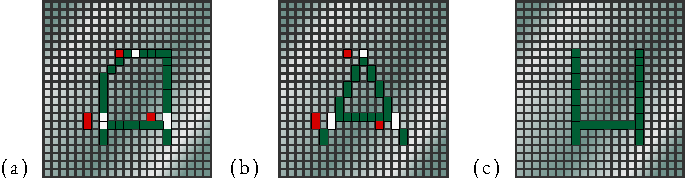
\includegraphics[width=\tfwidth]{figures/perceptron1.pdf}
\caption{Signals and their interpretations by a perceptron.\label{perceptron1}}
% fig 3.13
 \end{figure}
Secondly, the random nature of these relations suggests the \redem{adjustment}
of the perceptron to the patterns being recognized. A perceptron should
he presented with different images of the recognized patterns in turn
(and several times), and we should \redem{teach} it, the perceptron's parameters
being adjusted as needed in the process. A perceptron should take into
account its progress at each stage (at each presentation of the image), so
a perceptron should have a memory.

Considering both these points, we can define perceptrons to be
devices which have a memory and a random structure of the links
between its units. A perceptron can be thought of as a simplified model
of the brain, and this model is promising because it is \redem{probabilistic}, or,
in other words, \redem{stochastic}. Some scientists believe that stochastic models will be best able to simulate the processes occurring in the brain.
Various sorts of perceptron have been designed. Below we shall
consider a simple perceptron which can distinguish two patterns.

\txthead{The arrangement of the simplest perceptron.} A diagram of this
perceptron is given in \figr{perceptron2}. Here the $S_{i}$, are photoelectric cells (receptors), the $I_{k}$ are phase inverters, which change the sign of the electric voltage, the $A_{j}$ are associative units ($A$-units), the A. $\lambda_{j}$ are amplifiers with varying gain factors, $\Sigma$ is a summator, and $R$ is the receiver, Suppose that the total number of receptors $S_{i}$, is $N$, $(i = 1, \, 2, \, 3, \ldots{} , N)$. In the first models, $N$ was $20 \times 20 = 400$ receptors. The number of inverters is not fixed in that it can be different in different copies of the same device. The total number of associative units $A_{j}$ and amplifiers $\lambda_{j}$ equals $M \,\, (j = 1, \, 2, \ldots{} ,\, M)$. The receptors are wired to the $A$-units either directly or via the inverters. It is essential that the choice of which receptor is connected to which $A$-unit and the selection of the potential sign are random. Thus when a circuit is being assembled, the wires connecting the receptors to the $A$-units are soldered together \redem{randomly}, for instance, in accordance with instructions from a random
number generator.

\begin{figure}[ht]
 \centering
 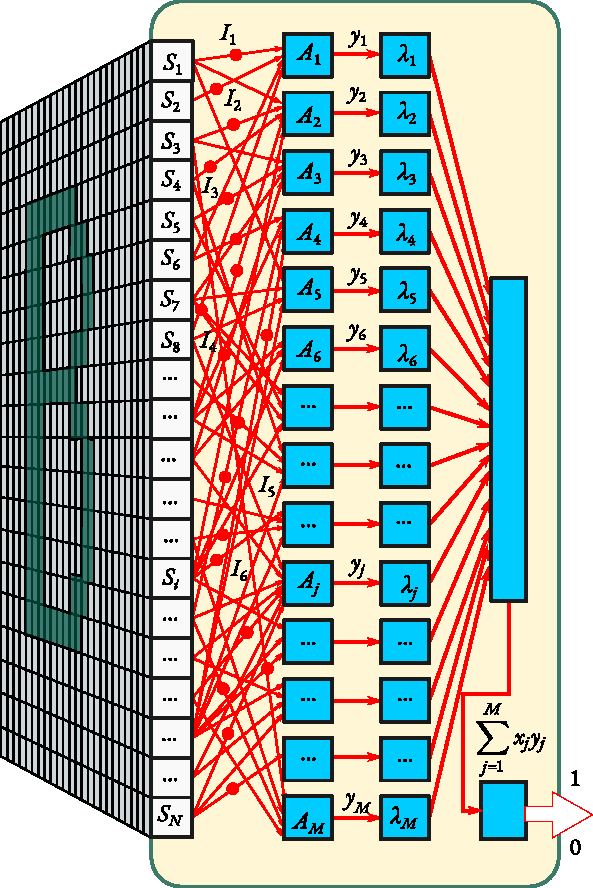
\includegraphics[width=.68\tfwidth]{figures/perceptron2.pdf}
\caption{Schematic diagram of the simplest perceptron.\label{perceptron2}}
% fig 3.13
 \end{figure}
 
Suppose that an image is projected onto the perceptron's sensor grid.
Since the intensity of the light at each point is different, some of the
receptors will be excited, generating a logic signal of 1, while others will
not, generating an electric signal of 0 at the output of the receptor. If the
signal passes through an inverter, a 1 is transformed into a $-1$. The
system of random links transmits the signals from the receptors to the
$A$-units. Each $A$-unit algebraically adds up the signals at its input. If the
sum is above a threshold, the output of the $A$-unit goes to logic + 1,
otherwise it goes to logic 0. Let us designate the signals leaving the
$A$-units $y_{j}$. Each $y_{j}$ is either + 1 or 0. The signal at the output of unit $A_{j}$ goes to the input of amplifier $\lambda_{j}$ and the amplifier transforms signal $v_{j}$ to a signal $\varkappa_{j} y_{j}$: The gain factor $\varkappa_{j}$ may vary both in absolute value and in sign. The signals from all the amplifiers are summed up in the summator $\Sigma$, and hence we get 
\begin{equation*}%
\sum_{j= 1}^{M} \varkappa_{j} y_{j}.
\end{equation*}
Then it is sent to the input of the $R$-unit, which checks its sign. If
$\sum_{j} \varkappa_{j} y_{j} \geqslant 0$, the $R$-unit output is + 1, otherwise the $R$-unit output is 0.

This perceptron is designed to recognize only two patterns.
Irrespective of the concrete images of the patterns, the perceptron will
respond to one pattern with an output signal of + 1 and with a signal
of 0 to the other. The perceptron must \redem{learn} this ability.

\txthead{Teaching a perceptron.} Let us call the two patterns $B$ and $C$. Suppose pattern $B$ corresponds to an output signal of + 1 and pattern $C$ to an output signal of 0. Suppose $\varkappa_{1}, \varkappa_{2}, \varkappa_{3},\ldots{} ,  \varkappa_{j},\ldots{}, \varkappa_{M}$ are the perceptron's gain factors before it is taught. Let us designate this ordered set $\{ \varkappa \}$. To teach the perceptron, we present it with an image of pattern $B$. This will excite a certain set of $A$-units, i. e. we get a succession of signals $y_{1}, y_{2}, y_{3},\ldots{} ,y_{j},\ldots{} , y_{M}$, or, in short, $\{ y \}$. Now suppose the sum $\sum_{j} \varkappa_{j} y_{j} $ is
non-negative, so the perceptron's output signal is + 1. If so, then
everything is true, and we can present the perceptron with a second
image of pattern $B$. The second image will excite a new set of $A$-units,
i.e. a new succession of signals $\{ y' \}$. The set of gain factors $\{ \varkappa \}$ remains yet the same, but the sum $\sum_{j} \varkappa_{j}' y_{j}' $ may be negative, and then the signal at the perceptron's output will be 0. This is not good, and therefore the perceptron is ``discouraged'': the gain factors of the excited $A$-units are incremented by, say, unity, so that a new set of gain factors $\{ \varkappa '\}$ ensures that the sum $\sum_{j} \varkappa_{j}' y_{j}' $ is non-negative. Now the perceptron responds correctly to the second image of pattern $B$. But what about the first image? The set of gain factors has been changed, so that the sign of the sum $\sum_{j} \varkappa_{j}' y_{j} $ may be changed. We present the perceptron with the first image of pattern $B$ again and identify the sign of the sum $\sum_{j} \varkappa_{j}' y_{j} $  by the output signal.

If the sum is non-negative, we are satisfied because the set of gain
factors $\{ \varkappa' \}$ has caused the perceptron to respond correctly to both the first and the second images of pattern $B$. Now we can present the
perceptron with a third image of pattern $B$. If the sum is negative, the
gain factors of the excited $A$-units should be incremented by unity again
(set $\{ \varkappa' \}$ is replaced by set $\{ \varkappa'' \}$), and so on.

Gradually, by varying the set of gain factors step by step, we will find
a set of factors such that the perceptron will produce a signal of + 1 for
any presented image of pattern $B$. However, our job is not yet over. It is
quite possible that after many increments of the various gain factors, the
perceptron will produce a + 1 signal for both pattern $B$ and pattern
$C$ images. However, the perceptron should produce a + 1 signal for all
pattern $B$ images and a 0 signal for all pattern $C$ images. This means
that while the perceptron is being taught, we should alternate between
both patterns and when presenting an image of pattern $C$, we should (if
need be) decrement rather than increment the gain factors of the excited
$A$-units to get $\sum x y$ below zero.

Ultimately, we will find a set of gain factors  $\{ \varkappa^{0} \}$ such that the perceptron will always recognize patterns $B$ and $C$. Suppose  $\{ y(n) \}$ is the set of excited $A$-units corresponding to an $n$th image of pattern
$B$ and  $\{ Y(m) \}$ is a set corresponding to an $m$th image of pattern $C$. The $M$ gain factors $\{ \varkappa^{0} \}$ should be such that 
\begin{equation*}
%\begin{split}
\sum_{j= 1}^{M} \varkappa^{0}_{j} y_{j} (n)  \geqslant 0 \,\, \text{for all} \,\, n \,\, \text{and} \,\,
\sum_{j= 1}^{M} \varkappa^{0}_{j} y_{j} (m)  \geqslant 0 \,\, \text{for all} \,\, m
%\end{split}
\end{equation*}

The teaching (and the learning) is over when such gain factors have been found.

\txthead{Conclusion.} In concluding this chapter, I went to emphasize the main
point, i.e. the deep, intrinsic relationship between \redem{information theory} and \redem{probability theory}. The very notion of information is underlain by
probability. And this is natural because control processes and random
processes are always \redem{dialectically united}. Randomness both ``steals''
information and generates it, because the most complicated information
devices are fundamentally based on random internal structures.

We see that the phrase ``the world is built on probability'', which is
the title of this book, has a deeper meaning. Mankind lives and acts in
a world filled with information. This information arises by nature
through probability and, moreover, is created in probabilistic processes.
Thus, a \redem{world filled with information} is naturally a \redem{world built on
probability}.
%%% Local Variables:
%%% mode: latex
%%% TeX-engine: xetex
%%% TeX-master: "twibop2"
%%% End:



\part{Fundamentality of the Probability Laws}
% !TEX root = twibop2.tex
\chapter{Probability in Classical Physics}
\epigraph{Probability theory is used in physics, and its first application of fundamental importance for our understanding of the laws of nature can be found in the general statistical theory of heat founded by Boltzmann and	 Gibbs \ldots{} 
The most elegant and important advantage of this theory is the understanding of thermodynamical ``irreversibility'' as a picture of transition to more probable states.}  {W. Pauli}

\section{Thermodynamics and Its Puzzles }


All bodies consist of molecules in chaotic thermal motion. This fundamental point can be disregarded when considering the basic problems of \redem{thermodynamics}, the branch of physics which seeks to derive, from a few basic postulates, relationships between the properties of matter, especially those which are affected by changes in temperature, and a description of the conversion of energy from one form to another.

Thermodynamics is a branch of physics in which the energy transfers between macroscopic bodies and their environment are investigated from the most general positions (without using molecular concepts). Thermodynamic considerations are underlain by a description of the states of the bodies using thermodynamic \redem{variables or the thermodynamic functions of state} or state parameters, and the use of several basic principles called the \redem{laws of thermodynamics}. You already know about such thermodynamic variables as \redem{temperature} and \redem{pressure}.

\txthead{Thermodynamic equilibrium.} Let us perform a simple experiment. Take a vessel with hot water into a room and put a thermometer into the water. By recording the readings of the thermometer over time, we will see that the temperature of the water gradually decreases until finally equals the air temperature in the room, after which the temperature will remain constant. This means that the water in the vessel has reached a \redem{thermodynamic (heat) equilibrium} with the environment. If a system is in a thermodynamic equilibrium, its thermodynamic functions of state (temperature and pressure) remain constant until disturbed. Another feature of a thermodynamic equilibrium is that the temperature is constant at all points of the system.


If a system does not exchange energy with bodies around it, it is a \redem{closed system}. When we talk about a thermodynamic equilibrium of a closed system, we mean an equilibrium between its various parts, each of which can be regarded as a macroscopic body.

Suppose we heat a body unevenly and then put it in a vessel which does not conduct heat. It can be said that we first disturb the thermodynamic equilibrium in the body and then leave it. The temperature of the hotter regions will decrease, and that of cooler ones will increase, and finally the temperature will become the same throughout the body: they will reach a thermodynamic equilibrium with each other. \redem{An unperturbed macro-system will always reach a state of thermodynamic equilibrium and remain there} until some external action brings it out of this state. If this action stops, the system will again reach a thermodynamic equilibrium.


And here is the first puzzle of thermodynamics. Why does a system brought out of thermal equilibrium and left to itself return to an equilibrium state, while systems in a thermal equilibrium and left to themselves do not leave it? Why is it not necessary to spend energy to maintain thermal equilibrium, while energy is needed to maintain a system in a thermodynamic equilibrium? By the way, this is a far from futile question. The weather outside may be below freezing, e.g. \SI{-1}{\degreeCelsius}, while it's warm in the room, \SI{+25}{\degreeCelsius}. The walls of houses conduct heat fairly well, and therefore, there is a non-equilibrium ``room-outside'' system. To maintain this thermodynamic non-equilibrium state, it is necessary to spend energy continuously to heat.

\txthead{The first law of thermodynamics.} A system may exchange energy with its environment in many ways, or, as is said, along many channels. For simplicity's sake, let us limit ourselves to a consideration of two channels, namely, the transfer of energy by \redem{heat conduction} and the transfer of energy by \redem{performing work}. The \redem{first law of thermodynamics} is simply the law of the conservation of energy involving the possible energy transfer between a body and its environment via different channels, i.e.
\begin{equation}%
\Delta \, U = A + Q,
\label{eq-4.1}
% eq 4.1
\end{equation}
where $ \Delta \, U = U_{2} - U_{1}$ is the change in the internal energy of the body ($U_{1}$ and $U_{2}$ being the internal energies of the initial and final states of the body, respectively), $A$ is the work performed by external forces with respect to the body, and $Q$ is the amount of heat transferred to or from the body by conduction. Note that unlike internal energy, which is a \redem{function of state} of the body (it varies when the body transfers from one state to another), neither work nor heat are functions of state. It is equally absurd to say that a body in a state has so much heat or so much work. The heat $Q$ and work $A$ in formula \eqref{eq-4.1} are the changes in the body's energy carried out through different channels. Let us consider a simple macro-system, an \redem{ideal gas} ($m$ is the mass of the gas). The internal energy of an ideal gas is proportional to the absolute temperature $T$ of the gas and does not depend on the volume $V$ it occupies. Let us change the gas volume using a piston. By pushing a close-fitting piston down a cylinder and thus compressing the gas in the cylinder, we perform some work $A$. When the gas expands, it performs	work 	$A'$ to move the piston back: $A' = - A$. This work is related to the change in the gas volume. It is numerically equal to the area under the pressure-volume curve, which describes the process, from $V= V_{1}$ to $V= V_{2}$, where $V_{1}$ and $V_{2}$ are the initial and final volumes of the gas.

Let us consider, from the viewpoint of the first law of thermodynamics, two types of gas expansion, \redem{isothermal} and \redem{adiabatic}. The former process occurs at constant gas temperature while the latter occurs when there is no heat exchange between the gas and the environment. The change in the gas volume should be carried out very slowly (compared to the rate at which thermal equilibrium is reached within the gas), and so the gas can be regarded at any moment in time as being in thermodynamic equilibrium. In other words, we assume that the gas passes from one thermodynamic equilibrium state to another, as it were, via a succession of intermediate equilibrium states.

If the expansion is \redem{isothermal}, the gas's temperature remains constant, and therefore, $\Delta U = 0 \,\, (U_{1} = U_{2})$. Noting this, we obtain from \eqref{eq-4.1}:
\begin{equation}%
- A = Q \quad \textrm{or} \quad A' = Q.
\label{eq-4.2}
\end{equation}
The expanding gas performs as much work as it receives heat from the environment during its expansion.

When the expansion is \redem{adiabatic}, there is no heat exchange with the environment ($Q = 0$). Therefore,
\begin{equation}%
\Delta \, U = A \quad \qor \quad A' = - \Delta \, U.
\label{eq-4.3}
\end{equation}
The expanding gas performs work owing to a decrease in its internal energy, and the gas's temperature therefore falls.

\begin{wrapfigure}[34]{o}{\mfwidth}
\centering
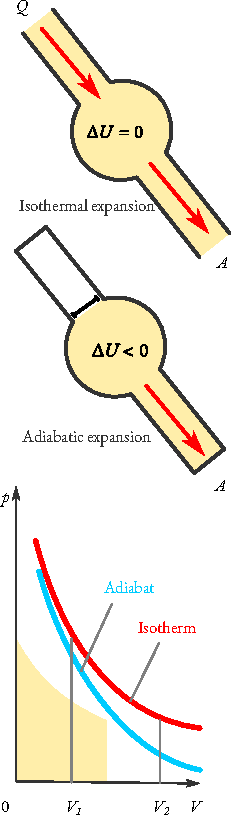
\includegraphics[width=0.8\linewidth]{figures/isotherm-adia.pdf}
\caption{Isothermal and adiabatic processes.\label{iso-adia}}
\end{wrapfigure}


Both of these processes are conventionally shown in \figr{iso-adia}. The processes are also represented on $p-V$ diagrams (where $p$ is the gas pressure). The work $A'$ performed by the gas in an isothermal expansion from volume $V= V_{1}$ to $V= V_{2}$ equals numerically the yellow area under the plot of $p (V)$ in the figure:
\begin{equation}%
A' = \int\displaylimits_{V_{1}}^{V_{2}} p(V) \, \dd V.
\label{eq-4.4}
\end{equation}
Using an equation of state for an ideal gas (the Mendeleev-Clapeyron equation), we get
\begin{equation}%
p= \frac{mRT}{MV},
\label{eq-4.5}
\end{equation}
where $M$ is the molar mass of the gas and $R$ is the universal gas constant. Substituting \eqref{eq-4.5} into \eqref{eq-4.4} and given that the temperature of the gas is constant, we obtain
\begin{equation}%
A = \frac{mRT}{MV} \int\displaylimits_{V_{1}}^{V_{2}} \frac{1}{V} \,\, \dd V = \frac{mRT}{MV} \, \ln \frac{V_{2}}{V_{1}},
\label{eq-4.6}
% eq 4.6
\end{equation}
(the symbol $\ln$ designates a logarithm to base $e = 2.71828 \ldots{}$). 



\txthead{The Carnot cycle.} In 1824, a 28-year-old engineer called Sadi, Carnot published a book in Paris entitled \redem{Refl\'exions sur la puissance moteurice du feu et Ie machine propre \`a developper cette puissance} (Reflections on the Driving Force of Fire and Machines Capable of Developing This Force). Unfortunately, his ideas as presented in the book were only appreciated many years later, and long after he had died. Carnot was investigating the work obtained from heat engines. He showed that a heat machine not only needs a hot body, it also requires a second body with a lower temperature. The first body is conventionally called the heat source, and the second is called the heat sink. Besides the heat source and heat sink, there must be a working substance (a liquid, steam, or gas), which transmits the heat from the heat source to the heat sink and performs work in the process. Carnot considered a closed cycle consisting of two isotherms and two adiabats. Later this cycle was called the \redem{Carnot cycle}. It is shown in \figr{ideal-gas} for an ideal gas. 

\begin{wrapfigure}{O}{\mfwidth}
\centering
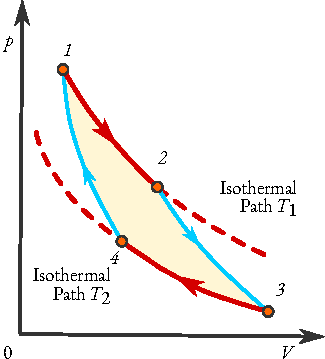
\includegraphics[width=\linewidth]{figures/carnot.pdf}
\caption{Carnot cycle for an ideal gas.\label{ideal-gas}}
\end{wrapfigure}

Suppose $T_{1}$, is the temperature of the heat source and $T_{2}$ is that of the heat sink. Moving from point 1 to point 2 (the isotherm for $T_{1}$ ), the gas receives a heat $Q_{1}$ from the heat source and expands, thus spending energy to perform work $A$. From point 2 to point 3 (along an adiabat), the gas performs work $A$; and its temperature falls to $T_{2}$. From point 3 to point 4 (the isotherm for $T_{2}$) the gas gives a heat $Q_{2}$ to the heat sink, and this heat equals the work $A_{2}$ performed to compress the gas. From point 4 to point 1 (another adiabat), the work $A_{4}$ is expended to compress the gas, and this goes to increasing the internal energy of the gas, so its temperature rises to $T_{1}$. The result is that the working substance returns to its initial state 1. 

Suppose that a heat engine operates following the Carnot cycle. The gas receives a heat $Q_{1}$ from the beat source and gives a heat $Q_{2}$ to the heat sink. In compliance with \eqref{eq-4.2}, we can write $Q_{1} = A'$ and $|Q_{2}| = A_{2}$. Note here that $Q > 0$ when heat is given to the gas, and that $Q < 0$ when the heat is taken from the gas. It is clear from \hyperref[ideal-gas]{Figure \ref{ideal-gas}} that the area under isotherm 3-4 is smaller than that under isotherm 1-2, and therefore, $A_{2} < A_{1}'$. Consequently, $|Q_{2}| < Q_{1}$ i.e. the gas gives the heat sink less heat than it receives from the heat source. At the same time, the internal energy of the gas, when the cycle is completed, remains the same. Therefore, the difference $Q_{1} - |Q_{2}|$ equals the work performed by the heat engine during its cycle. Hence the
efficiency of the heat engine is 
\begin{equation}%
\eta = \frac{(Q_{1} - |Q_{2}|)}{Q_{1}}.
\label{eq-4.7}
\end{equation}
Carnot showed that
\begin{equation}%
\frac{Q_{1}}{T_{1}} = \frac{(|Q_{2}|)}{T_{2}}.
\label{eq-4.8}
\end{equation}
This allows us to rewrite \eqref{eq-4.7} in the form 
\begin{equation}%
\eta = \frac{(T_{2} - T_{1})}{T_{1}}.
\label{eq-4.9}
\end{equation}
The efficiency of a heat engine, as defined by \eqref{eq-4.7} and \eqref{eq-4.9}, is the best possible efficiency. The efficiency of real heat engines is always less because of unavoidable irreversible processes.

\txthead{Reversible and irreversible processes.} The notions of reversible and irreversible processes are essential for thermodynamics. A process is said to be \redem{reversible} if the system (the working substance) is in thermal equilibrium all the time, continuously passing from one equilibrium state to another. This process is completely controlled, while it lasts, by the changes in its parameters, for instance, the temperature or volume. If the parameters are changed in the reverse direction, the process will also go backwards. Reversible processes are also called \redem{equilibrium processes}.

Boyle's (Mariotte's) and Gay-Lussac's (Charles') laws define reversible processes in an ideal gas. The expressions \eqref{eq-4.7} and \eqref{eq-4.9} we have just obtained are related to a reversible Carnot cycle, which is also called the ideal Carnot cycle. Each part of the cycle and the whole cycle can be reversed if desired.

An \redem{irreversible} process is a process that cannot be controlled. It proceeds independently, or, in other words, spontaneously. The result is that we cannot reverse such a process. It was noted above that once a system is moved from its thermodynamic equilibrium, it tends spontaneously to another thermodynamic equilibrium state. Processes related to transition of a system from a non-equilibrium state to an equilibrium one are irreversible. They are also called \redem{non-equilibrium} processes.

Here are some examples of irreversible processes: conduction of heat from a hotter body to a cooler one, mixing of two or more gases in the same vessel, expansion of a gas in vacuum. All of these processes occur spontaneously, without any external control. Heat does not spontaneously transfer from a cooler body to a hotter one. The components of a gas mixture do not spontaneously separate. A gas cannot spontaneously compress. I wish to emphasize: \redem{every irreversible process is characterized by a definite direction}. It develops in a certain direction and does not develop in the opposite one. Which direction a process can develop along and which it cannot are problems related to the second law of thermodynamics.

\txthead{The second law of thermodynamics.} One of the first formulations of the \redem{second law of thermodynamics} was given by the English physicist William Thompson (Lord Kelvin):
\begin{quote}
``It is \redem{not} possible that, at the end of a cycle of changes, heat has been extracted from a reservoir and an equal amount of work has been produced without producing some other effects.''
\end{quote}
This means that it is impossible to design a machine to carry out work by reducing the internal energy of a medium, sea water, for instance. Kelvin called such a machine a \redem{perpetuum mobile of the second kind}. While some \redem{perpetua mobile} violate the law of the conservation of energy (\redem{perpetua mobile of the first kind}), those of the second kind do not contradict the first law of thermodynamics; they are instead forbidden by the second law.	

In 1850, the German physicist Rudolf Clausius formulated the second law of thermodynamics as follows: 
\begin{quote}
``The transfer of heat from a cooler body to a hotter one cannot proceed without compensation.'' 
\end{quote}
It is useful to demonstrate the equivalence of the formulations given by Kelvin and Clausius. If we could, despite Kelvin's formulation, ``extract'' heat from a medium and, using a cyclic process, turn it into work, then, using friction, transform this work into heat at a higher temperature, we would contradict Clausius's formulation because it would involve the conduction of heat from a cooler body to a hotter one within a closed cycle without any external force performing work.

On the other hand, suppose that, despite Clausius's formulation, we succeed in getting some quantity of heat $Q$ to conduct itself from a cooler body (at a temperature $T_{2}$) to a hotter one ($T_{1}$), and subsequently, allow this heat to go naturally from the hotter body to the cooler at the same time performing some work $A'$ while the rest of the heat $Q_{1} = Q - A'$ returns to the cooler body. This process is shown in \figr{perp}~\drkgry{(a)}. It is clear that this process corresponds to direct transformation of heat $Q - Q_{1}$ into work $A$ (\figr{perp}~\drkgry{(b)}), which evidently contradicts Kelvin's formulation.

\begin{wrapfigure}{O}{\mfwidth}
\centering
\includegraphics[width=\linewidth]{figures/perp.pdf}
\caption{Work done in transfer of heat from bodies at different temperatures.}
\label{perp}
\end{wrapfigure}

\txthead{Entropy.} As he was studying Carnot's investigations, Clausius discovered that relationship \eqref{eq-4.8} is similar to a conservation law. The value of $Q_{1}/T_{1}$ ``taken'' by the working substance from the heat source equals the  $|Q_{2}|/T_{1}$ ``conducted'' to the heat sink. Clausius postulated a variable $S$, which like the internal energy is a state function of the body. If the working substance (an ideal gas in this case) receives heat 
$Q$ at temperature $T$, then $S$ is incremented by
\begin{equation}%
\Delta S= Q/T.
\label{eq-4.10}
\end{equation}
Clausius called $S$ \redem{entropy}. 

From point 1 to point 2 of the Carnot cycle (see \figr{ideal-gas}), a heat $Q_{1}$ is conducted from the, heat source to the working substance at a temperature $T_{1}$, and the entropy of the working substance increases by $\Delta S_{1} = Q_{1}/T_{1}$. From	 point 2 to point 3	and from point 4 to point 1, there is no conduction of heat, and therefore, the entropy of the working substance does not vary. From point 3 to point 4, a heat $Q_{2}$ is conducted from the working substance to the heat sink at temperature $T_{2}$, and	the	entropy of the	body is decreased by	$| \Delta S_{2}| = |Q_{2}| /T_{2} \,\, (\Delta S_{2} < 0)$. According to \eqref{eq-4.8} and \eqref{eq-4.10}), 
\begin{equation}%
\Delta S_{1} + \Delta S_{2} = 0.
\label{eq-4.11}
% eq 4.11
\end{equation}
Consequently, when an ideal (reversible) Carnot cycle comes to an end, the working substance's entropy returns to its initial value. 

Note that entropy can be defined as the state function of a body (system) whose value remains constant during an adiabatic process. Similarly, temperature can be regarded as the state function of a system whose value remains constant during an isothermal process. 

We shall later need to deal with a property of entropy called its additivity. This means that the entropy of a system is the sum of the entropies of the system's parts. Mass, volume, and internal energy are also additive. However, neither temperature nor pressure are additive.

\txthead{The second law of thermodynamics as the law of increasing entropy in irreversible processes within closed systems.} Using the notion of
entropy, we can formulate the second law of thermodynamics as follows:
\begin{mybox}{}
Any irreversible process in a closed system proceeds so that the system's entropy increases.
\end{mybox}
Consider the following irreversible process by way of an example. Suppose a closed system consists of two subsystems 1 and 2 which are at temperatures $T_{1}$ and $T_{2}$, respectively. Suppose that an infinitesimal amount of heat $\Delta Q$ is conducted from subsystem 1 to subsystem 2, so that the temperatures of the subsystems almost remain the same. The entropy of subsystem 1 reduces by $ \Delta Q/T_{1}$, $(S_{1} = - \Delta Q/T_{1})$ while the entropy of subsystem 2 increases by $\Delta S_{2} = \Delta Q/T_{2}$ The entropy of the whole system is the sum of its subsystems' entropies, and therefore, the change in the system's entropy will be
\begin{equation}%
\Delta S =  \Delta S_{1} + \Delta S_{2} = \Delta Q \left( \frac{1}{T_{2}} - \frac{1}{T_{1}} \right).
\label{eq-4.12}
\end{equation}
Heat conduction from subsystem 1 to subsystem 2 is irreversible if $T_{1} > T_{2}$. Using this inequality, we can conclude from \eqref{eq-4.12} that $\Delta S > 0$. Thus, we see that the process of heat conduction from a heated body to a cooler one is accompanied by an increase in the entropy of the system consisting of the two.

A gain in entropy during irreversible processes is only a necessary law for closed systems. If a system is open, a reduction in its entropy is possible. Thus, if some external body does work with respect to the system, heat can be transferred from a heat sink to a heat source. It is essential that if the system includes a heat source, a heat sink, a working substance, and all the bodies that perform work (i.e. if we consider a closed system again), then. the total entropy of this system will increase.

I shall now formulate the basic conclusions concerning the change in the system's entropy.

\redem{The first conclusion.} If a system is closed, its entropy does not decrease over time:
\begin{equation}%
\Delta S \geqslant 0.
\label{eq-4.13}
\end{equation}
The system's entropy does not vary if the processes within it are reversible. If the processes are irreversible, the system's entropy increases. The gain in entropy can be regarded as a measure of the irreversibility of the processes occurring in it.

\redem{The second conclusion.} Generally, nothing can be said about the change in entropy in an open system. It can either remain constant or increase or even decrease.

\txthead{The puzzles of thermodynamics.} These puzzles focus on the second law of thermodynamics. Since it gives a definite direction to the processes in nature, it introduces a fundamental irreversibility. How can this irreversibility be explained by physics? Why can heat be transferred from a hotter body to a cooler one while it cannot be spontaneously conducted in the opposite direction? Why does any gas expand in vacuum but does not compress spontaneously? Why, when in the same vessel, do two or more gases mix, but not spontaneously separate? A hammer strikes an anvil. The temperature of the anvil rises a bit. But however strongly we might heat the anvil with the hammer resting on it, the reverse will not happen: the hammer will not jump off the anvil. Why? Very many similar ``whys'' can be asked. Thermodynamics does not answer these questions in principle. The answer must be sought in the kinetic theory of matter. We should now look into the picture of chaotically moving molecules.

\section{Molecules in a Gas and Probability }

\txthead{A dialogue with the author.} Imagine that we are talking with a physicist of the 1860s. We do not need a ``time machine''. We shall just believe that my partner adheres to the views typical of physicists in the mid-$19^{\text{th}}$ century, the same physicists, many of whom later, in the 1870s, could not understand or accept the ideas of the Austrian physicist Ludwig Boltzmann (1844-1906). Anyway, let us imagine that it is 1861. 

\begin{dialogue}

\athr ``Let us consider a gas to be an ensemble of very many
chaotically moving molecules.''

\prtnr ``Good. I'm aware of the recent investigations of James
Clerk Maxwell, who calculated the velocity distribution of molecules
in a gas.'' 

\athr ``I would like to discuss some thing more fundamental than
the distribution established by Maxwell. The point is that there is a qualitative difference between considering thermodynamic equilibria and considering the motion of molecules. In the first we have \redem{dynamic} laws with strictly determined dependences, and in the second we have the \redem{probabilistic} laws that govern processes in large ensembles of molecules.''

\prtnr	``But the movements of molecules are governed by Newton's laws of classical mechanics rather than by probabilistic laws. Suppose we assign coordinates and velocities to all the molecules in a gas at a certain moment. Suppose that we can follow all the collisions of the molecules with each other and with the walls of the vessel. It is clear that in this case we will be able to predict where a molecule will be at some other moment and what velocity it will have.''


\athr ``Why aren't you bothered by the fact that you're very much like the superbeing of which Laplace wrote?''

\prtnr ``I have a concrete problem in mechanics. True, the number of bodies is extremely great.''

\athr ``There are about \num{d19} molecules in a cubic centimetre of gas under normal conditions. You have a problem in which some \num{d20} bodies have to be accounted for.''

\prtnr ``Naturally, it would be exceptionally difficult. But the difficulty is purely technical and not fundamental. So long as our calculational abilities are limited, we shall have to resort to probabilities, the probability of a molecule arriving in a volume, its probability of having a velocity in a certain range, etc.''


\athr ``Thus, you believe that the use of probabilities is only related to our practical inability to perform a very cumbersome calculation, but that in principle an ensemble of molecules behaves according to Newton's laws as applied to individual molecules.''

\prtnr ``Precisely. This is why I do not see the qualitative difference you mentioned.''

\athr ``I have at least three hefty arguments to support my position that the probabilistic description of large ensembles of molecules is necessary in principle, that chance is present in the very nature of these ensembles rather than simply being related, as you seem to believe, with our inadequate knowledge and inability to perform cumbersome calculations.''

\prtnr ``I'd like to know of these arguments.''

\athr ``I'll start with the first. Suppose there is, as you postulate,
a rigid system of strictly determined links (as given by Newton's laws) between the molecules in a gas. Now imagine that some of these molecules suddenly escape from this system (e.g. they escape from the vessel through a slit). Clearly the disappearance of these molecules will bring about the disappearance of all that is predetermined by their presence, I mean their later collisions with other molecules, which, in its turn, will change the behaviour of the other molecules. All this will affect the whole system of rigid relationships and, as a consequence, the behaviour of the ensemble as a whole. However, we know that from the viewpoint of gas as a whole you can suddenly withdraw a large number of molecules without any noticeable effect (for instance, \num{d12} molecules or more). The properties of the gas and its behaviour do not change in the least. Does this not indicate that the dynamic laws governing the behaviour of individual molecules do not actually interfere with the behaviour of the gas as a whole?"

\prtnr ``Still, it is hard to believe that molecules obey some laws while the ensemble of the same molecules obeys quite different laws.''




\athr ``But this is exactly so. And my second argument will emphasize this fundamental point. I'll give you some simple examples. A stone is thrown from point $A$ at some angle to the horizontal (\figr{reflect}~\drkgry{(a)}). Imagine that we can change the direction of the stone's velocity to the opposite at point $B$ of its trajectory. It is clear that the stone should return to point $A$ and have the same velocity (in absolute value) it had when it was thrown. The flying stone, as it were, `remembers' its history.''

\prtnr ``This is natural because each state of the thrown stone is
determined by its preceding one and, in its turn, determines the subsequent one.''

\athr ``Another example: a ball hits a wall elastically and bounces
off (\figr{reflect}~\drkgry{(b)}). If you change the direction of the ball's velocity to the opposite one at point $B$, the situation will recur in the reverse order: the ball will hit the wall and return to point $A$.

``I cited these examples in order to illustrate an essential idea: the movements determined by the laws of classical mechanics have a kind of ``memory'' of the past. This is why these movements can be reversed.''

``Another thing is the behaviour of gas. Imagine the following situation. There is a beam of molecules whose velocities are parallel. After entering a vessel, the molecules collide many times with each other and the walls. The result is that the molecules reach a state of thermodynamic equilibrium, and they lose all `memory' of their past. It can be said that any gas in a state of thermal equilibrium, as it were, `forgets' its prehistory and does not `remember' how it arrived at the equilibrium state. Therefore, it is absurd to think of reversing the situation: the molecules could not recollect into a beam and depart from, the vessel in one definite direction. Many examples of such forgetfulness can be cited.''

``Suppose there is some gas on one side of a partition in a vessel and another gas is on the other side. If you take away the partition, the molecules of both gases will mix. Evidently, we should not expect this picture to reverse: the molecules will not move back into their own halves of the vessel. We might say that the mixture of two gases does not remember its prehistory.''

\prtnr ``Do you want to say that the equilibrium state of a gas is not predetermined by the preceding states of the gas?''

\athr ``When we use the word predetermined, we mean strictly unambiguous predetermination. There is no such predetermination here. A gas may arrive in an equilibrium state from different initial states. No information may be obtained about the initial states by studying the gas in thermal equilibrium. This means that the gas forgets its prehistory.''

\prtnr ``Yes, this is true.''

\athr ``And when does this loss of memory occur? It occurs when \redem{chance} comes into play. You throw a die, and, say, a four turns face up. You throw again and a two appears. The appearance of the two is not related to the appearance of the four before it. You throw the die many times and obtain a set of digits. This set possesses stability (for instance, the four occurs approximately in one-sixth of all trials). This stability does not have any prehistory, it is not related to the occurrence of any other digit in the previous trials.''

``The same happens in a gas. The loss of prehistory indicates that we must deal with \redem{statistical} laws, laws in which chance plays a fundamental role.''

\prtnr ``It seemed to me before that everything was clear. Newton developed his mechanics. Then the temperature and pressure of gas appeared. Using the notion of molecules, we reduced these physical variables to mechanical ones by relating temperature to the energy of molecules and the pressure of the gas to the impulses transferred to the wall by the molecules striking it. Therefore, the laws of mechanics were and continue to be fundamental laws. Are you suggesting we put probabilistic laws on the same level as the laws of mechanics?''

\athr ``I believe that you are aware of the fact that some thermodynamic variables do not have analogues in classical mechanics. And here is my third argument. Entropy does not have a mechanical analogue. The very existence of a variable such as entropy is sufficient to disprove the thesis of the total fundamentality of the laws of classical mechanics.''

\prtnr	``I would not like to discuss entropy at all \ldots{}'' 


\end{dialogue}

\begin{wrapfigure}{O}{\mfwidth}
\centering
\includegraphics[width=\linewidth]{figures/reflect.pdf}
\caption{Bounce of a stone and an elastic ball.\label{reflect}}
\end{wrapfigure}

Let us finish with this dialogue because it has become a bit too long. We agreed that it referred to 1861. Therefore, I could not use arguments that were unknown at the time. But here I can cite two more arguments in favour of my position. Firstly, note that entropy is explicitly expressed in terms of probability, and that namely this makes it possible to explain every puzzle of thermodynamics. We shall discuss this in detail in the next sections. Secondly, it follows from quantum physics that the assumption (made by my partner) that he can assign coordinates and velocities to all the molecules simultaneously proves to be inconsistent. This cannot be done due to fundamental considerations, which we shall talk about in detail in Chapter 5. 

And now let us discuss molecules moving in a gas.

\txthead{Movements of gas molecules in thermodynamic equilibrium.} Suppose a gas of mass $m$ is in thermal equilibrium. The gas occupies volume $V$ and has temperature $T$ and pressure $p$.

Each gas molecule moves with a velocity which is constant in magnitude and direction until the molecule collides with either another molecule or the wall. On the whole, the picture of molecular movements is chaotic: the molecules move in different directions with different velocities, there are chaotic collisions leading to changes in the direction of movement and the absolute value of the velocities of molecules. Let us take an imaginary ``photograph'' of the molecules' positions at a single moment in time. It might look like the one in (\figr{mol-photo}), where for simplicity's sake only two rather than three dimensions are considered (the ``photograph'' is flat). It is clear that the points (molecules) fill the volume of the vessel uniformly (the vessel in the figure is the square). Suppose $N$ is the total number of molecules in the vessel; $N=N_{A}m /M$, where $N_{A}$ is Avogadro's number. At any site within the vessel and at any moment in time, the number of molecules per unit volume is the same (on average), $N/V$. Molecules may be found with equal probability at any point within the vessel.
\begin{wrapfigure}{O}{\mfwidth}
\centering
\includegraphics[width=0.95\linewidth]{figures/mol-photo.pdf}
\caption{A snapshot of the molecules in motion.\label{mol-photo}}
% fig 4.5
\end{wrapfigure}

Let us use $G (x, y, z) \, \Delta dx \, \Delta dy\, \Delta dz$ to denote the probability of finding a molecule within a volume $ \Delta V = \Delta x \, \Delta y \, \Delta z$ in the vicinity of a point with coordinates $(x, y, z)$. To be more accurate, this is the probability that the $x$-coordinate of the molecule will take a value from $x$ to $x + \Delta x$, its $y$-coordinate from $y$ to $y + \Delta y$, and its $z$-coordinate from $z$ to $z + \Delta z$. At small $ \Delta x, \, \Delta y$, and $ \Delta z$, the function $G(x, y, z)$ will be the density of the probability of finding a molecule at point $(x, y, z)$. The probability density in this case does not depend on the coordinates, hence $G = \text{const}$. Since the probability of finding a molecule somewhere within the vessel is unity, we have
\begin{equation*}%
\int\limits_{V} G \, \dd V =1,  \qor  G \int\limits_{V}  \dd V = GV = 1.
\end{equation*}
Consequently, $G = 1/V$. 

Wherever a unit volume is taken within the vessel, the probability of finding a molecule within the unit volume is $1/V$, i.e. the ratio of the unit volume to the volume of the vessel. Generalizing this conclusion, we can state that the probability of finding a molecule within volume $V_{0}$ is $V_{0}/V$.

\begin{wrapfigure}{O}{\mfwidth}
\centering
\includegraphics[width=\linewidth]{figures/mol-dist.pdf}
\caption{A snapshot of molecular velocity distribution.}
\label{mol-dist}
% fig 4.6
\end{wrapfigure}

Now let us discuss the velocities of the gas molecules. It is clear from the start that the velocities cannot all be equally probable: there should be few molecules with very high and very small velocities. When considering the velocities of molecules, it is convenient to use the concept of a \redem{velocity space}, i.e. the molecular velocities are projected onto the coordinate axes $v_{x}, v_{y}, v_{z}$. For simplicity's sake, \figr{mol-dist} shows only two axes: the $v_{x}$-axis and the $v_{y}$-axis (a two-dimensional velocity space). The figure shows a molecular velocity distribution in a gas for some moment in time. Each point in the figure relates to a molecule. The abscissa of the point is the $x$-projection of the molecule's velocity and the ordinate is its $y$-projection.

It is interesting to compare \figr{mol-photo} and \figr{mol-dist}. The points in \figr{mol-photo} are within a certain area and the distribution is uniform. The scatter of points in \figr{mol-dist} is unlimited in principle. These points clearly focus around the origin. This means that although the projection of a molecule velocity may be as large as you wish, the projections of the velocities in the neighbourhood of zero are the most probable. The scattering in \figr{mol-dist} is rotationally symmetric for any angle about the origin. This means that all directions of movement are equally probable: a molecule may be found moving in any direction with equal probability.

In order to have a correct picture of the molecular movements in a gas, we should use both figures. It is still better, instead of each figure, to consider a sequence of snapshots taken at regular intervals in time.

We should then see that the points in \figr{mol-photo}  move in different directions: the trajectories change during collisions. The points in \figr{mol-dist} do not move; however, some suddenly disappear and some appear. Each time a pair of points disappears another pair of new points appears: this is the result of collision between two molecules.

\txthead{Maxwell's distribution law.} Suppose $F  (v_{x}) \Delta v_{x}$ is the probability that a certain molecule (at a certain moment in time) has an $x$-velocity component	from	 $v_{x}$	to	$v_{x} + \Delta v_{x}$	the	other two	velocity components taking any arbitrary value. At small $\Delta v_{x}$ the function $F  (v_{x})$ is the density of the probability of finding a molecule with velocity component $v_{x}$.

The English physicist James Clerk Maxwell (1831 -1879) showed that
the	probability	density	 $F  (v_{x})$ corresponds	to \redem{Gauss's law}:
\begin{equation}%
F (v_{x}) = A \, \exp (- \alpha \, v_{x}^{2}),
\label{eq-4.14}
\end{equation}
where $\alpha$ is a parameter ($\alpha > 0$) and the constant $A$ is determined from
\begin{equation}%
\int\limits_{- \infty}^{\infty} F (v_{x}) \dd v_{x} = 1,
\label{eq-4.15}
\end{equation}
which is a reflection of the fact that the probability of a molecule having
an $x$-component in its velocity is unity. Substituting \eqref{eq-4.14} into \eqref{eq-4.15}, we obtain
\begin{equation*}%
A \, \int\limits_{- \infty}^{\infty} \exp (- \alpha \, v_{x}^{2}) \dd v_{x} = 1.
\label{gauss-law-param}
\end{equation*}
The integral in this expression is known in mathematics as Poisson's integral and, evaluates to $\sqrt{\pi / \alpha}$. Consequently, $ A = \sqrt{\pi / \alpha}$. Thus, we can rewrite \eqref{eq-4.14} as 
\begin{equation}%
F (v_{x})  = \sqrt{\pi / \alpha} \, \exp (- \alpha \, v_{x}^{2}).
\label{eq-4.16}
\end{equation}
Similar functions can be derived for the probability densities for the $y$- and $z$-components of a molecule's velocity. The function $F(v_{x} )$ is plotted in \figr{gauss-dist}. Suppose $f \,(v_{x}, v_{y}, v_{z})$ is the density of the probability of finding a molecule with velocity components $v_{x}, v_{y}$, and $v_{z}$. Using the theorem of probability multiplication, we can write:
\begin{equation*}%
f \, (v_{x}, v_{y}, v_{z}) \, \Delta v_{x}\, \Delta  v_{y} \, \Delta v_{z} = [F(v_{x} \Delta \, v_{x})] [F(v_{y} \Delta \, v_{y})][F(v_{z} \Delta \, v_{z})].
\end{equation*}
Whence
\begin{equation}
f \, (v_{x}, v_{y}, v_{z}) = \left(\frac{\alpha}{\pi} \right) ^{3/2} \, \exp (- \alpha (v_{x}^{2}+ v_{y}^{2} + v_{z}^{2})) = \left(\frac{\alpha}{\pi} \right) ^{3/2} \, \exp(- \alpha v^{2}).
\label{eq-4.17}
\end{equation}

\begin{figure}[!ht]
\centering
\includegraphics[width=0.75\tfwidth]{figures/maxwl-dist1.pdf}
\caption{The Gauss velocity distribution.\label{gauss-dist}}
\end{figure}



We see that the probability density depends on the squares of the velocity components, viz. $v_{x}^{2}+ v_{y}^{2} + v_{z}^{2}= v^{2}$. This we might have expected because, as it was already noted, each velocity direction is equally probable, and so the probability density may only depend on the absolute value of a molecule's velocity.

Thus, the probability of finding a molecule with velocity components taking the values $v_{x} - v_{x} + \, \Delta v_{x}, \,\, v_{y} - v_{y} + \, \Delta v_{y}, \,\,v_{z} - v_{z} + \, \Delta v_{z}, \,\,$ is:
\begin{equation}%
\Delta w_{v}  = \left(\frac{\alpha}{\pi} \right) ^{3/2} \, \exp (- \alpha v^{2})  \Delta v_{x} \Delta v_{y} \Delta v_{z},
\label{eq-4.18}
\end{equation}
where $v^{2} = v_{x}^{2}+ v_{y}^{2} + v_{z}^{2}$.

	
\begin{figure}[!ht]
\centering
\includegraphics[width=0.9\tfwidth]{figures/velspace.pdf}
\caption{The velocity space.\label{vel-space}}
% fig 4.8
\end{figure}
Let us take one more step: since each velocity direction is equally probable, let us look at the probability of finding a molecule with an absolute	velocity from $v$ to $v + \Delta v$,	irrespective of	its direction. If	we consider a velocity space (\figr{vel-space}), then $\Delta w_{v}$ (see \eqref{eq-4.18}) is the probability of finding a molecule in the ``volume'' $\Delta v$, shown in (\figr{vel-space}~\drkgry{(a)}) (the word ``volume'' is enclosed in quotation marks to remind us that we are dealing with a velocity space rather than with a normal space). Now we want to consider the probability of finding a molecule within the spherical layer shown in \figr{vel-space}~\drkgry{(b)} and confined between spheres with radii $v$ and $v + \Delta v$. The ``volume'' of this layer is the surface area of a sphere of radius $v$ multiplied by the thickness of the layer $\Delta v$, i.e. $4 \pi v^{2} \Delta v$. Therefore, the probability we want has the form:
\begin{equation}%
\Delta w_{v}  = \left(\frac{\alpha}{\pi} \right) ^{3/2} \exp (- \alpha v^{2})  4 \pi v^{2} \Delta v.
\label{eq-4.19}
\end{equation}
This formula expresses the distribution of molecules in an ideal gas by the absolute value of their velocities, i.e. the \redem{Maxwellian distribution}. The probability density $g (v) = \Delta w_{v} / \Delta v$ is shown in \figr{mxwl-space}. It vanishes both when $v$ tends to zero and when it tends to infinity. The ``volume'' of the spherical layer shown in \figr{vel-space}~\drkgry{(b)} vanishes when $v$ tends to zero and the factor $\exp(- \alpha v^{2})$ in the distribution law vanishes when $v$ tends to infinity.
\begin{figure}[!ht]
\centering
\includegraphics[width=0.8\tfwidth]{figures/dist2.pdf}
\caption{The Maxwellian velocity distribution.\label{mxwl-space}}
% fig 4.9
\end{figure}

\txthead{Chance and necessity in the pattern of moving molecules.} Suppose we could record the position and velocity of every molecule in a volume of gas at some moment in time. Imagine now that we divide the volume into numerous identical cells, and look at our instantaneous ``photograph'' from cell to cell. It will turn out that the number of molecules varies from cell to cell in a random fashion. Let us only pay attention to those molecules whose velocities are within the range from $v$ to $v + \Delta v$. The number of such molecules varies randomly from cell to cell. Let us divide the solid angle for all space at a point, i.e. $4 \pi$ steradians, into many identical elementary solid angles. The number of molecules whose velocities lie within an elementary solid angle varies randomly from one such an angle to another.

We could look at the situation in another way, that is, we could focus our attention on some cell or an elementary solid angle and take snapshots at different moments in time. The number of molecules (in a cell or a solid angle) at different times will also randomly change.

To emphasize the \redem{randomness} in the picture of moving molecules, the term ``chaotic'' is applied: chaotic collisions between molecules, chaotically directed molecule velocities, or generally, the chaotic thermal
movement of molecules. However, there is some \redem{order} in this ``chaos'' or, in other words, \redem{necessity} or what we have repeatedly called \redem{statistical stability}.

The statistical stability shows itself in the existence of definite probabilities: the probability of a molecule being in a volume $\Delta V$ (the probability is $\Delta V/ V$), the probability of a molecule moving within a solid angle $\Delta \Omega$ (the probability is $\Delta \Omega/4\pi$), and the probability of a molecule having an absolute value of velocity from $v$ to $v + \Delta v$ (the probability is defined by \eqref{eq-4.19}).

The number of molecules per unit volume each possessing an absolute value of velocity from $v$ to $v + \Delta v$ is, to a great degree of accuracy,
\begin{equation}%
\Delta n = \frac{N}{V} \, \Delta w_{v}  =  4 \pi \, \frac{N}{V}  \left(\frac{\alpha}{\pi} \right) ^{3/2} \, \exp (- \alpha v^{2}) \, 4 \pi v^{2} \Delta v.
\label{eq-4.20}
% eq 4.20
\end{equation}
Collisions between molecules push some molecules out of this range of velocity values; however, other collisions bring new molecules into it. So order is maintained: the number of molecules in a given interval of velocity values remains practically constant and is defined by \eqref{eq-4.20}. Let me emphasize that chance and necessity, as always, are dialectically united here. Collisions among a great number of molecules give the picture of the moving molecules its randomness. But at the same time the collisions maintain the thermodynamic equilibrium in the gas, which is characterized by definite probabilities, and in turn reveals statistical stability.

\section{Pressure and Temperature of an Ideal Gas}

\txthead{Pressure as the result of molecular bombardment.} The walls of a vessel containing a gas are continuously struck by gas molecules. This molecular bombardment results in the pressure exerted by a gas on a wall. Let us take an $x$-axis at right angles to the wall. It is clear from \figr{collisions}~\drkgry{(a)} that the $x$-component of a molecule's momentum in an elastic collision with the wall changes by $2m_{0}v_{x}$ where $m_{0}$ is the mass of the molecule. This means that when it strikes the wall, the molecule gives it an impulse of $2m_{0}v_{x}$. Let us first look at those gas molecules whose $x$-components of velocity lie between $v_{x}$ and $v_{x} + \Delta v_{x}$ (note that $v_{x} > 0$, otherwise the molecule will be moving away from the wall rather than towards it); the other components of the molecule's velocity are not important. The number of collisions between the molecules in question and an area $s$ of the wall per unit time equals the number of molecules in a volume equal to $s v_{x}$ \figr{collisions}~\drkgry{(b)}. (The reader should not be confused by the fact that the product $s v_{x}$ does not have the dimensions of volume. In reality, we deal herewith the product $s(\si{\centi\meter\squared}) \times v_{x} (\si{\centi\meter\per\second}) \times 1 (\si{\second})$.) Regarding \eqref{eq-4.16}), this number of collisions is
\begin{equation*}%
\Delta R = \frac{N}{V} \, s\, v_{x} F(v_{x}) \, \Delta v_{x} =  \frac{N}{V} \, s\, v_{x} \sqrt{\frac{\alpha}{ \pi}} \, \exp (- \alpha v_{x}^{2}) \, \Delta v_{x}.
\end{equation*}

\begin{figure}[!ht]
\centering
\includegraphics[width=0.8\tfwidth]{figures/collisions.pdf}
\caption{The collisions of molecules with walls of the container.\label{collisions}}
% fig 4.10
\end{figure}

The wall receives an impulse of  $2m_{0}v_{x}$ at each collision. The force acting on an area $s$ of the wall per unit time is the impulse transferred to the area. Dividing the force by the area $s$, we can find the pressure exerted by the gas on the wall caused by the molecules whose $x$-velocity components take values from $v_{x}$ to $v_{x} + \Delta v_{x}$:
\begin{equation}%
\Delta p = 2m_{0}v_{x} \Delta R  \frac{1}{s} =  2m_{0} \frac{N}{V} \, \sqrt{\frac{\alpha}{ \pi}} \exp (- \alpha v_{x}^{2}) \, v_{x}^{2} \, \Delta v_{x}.
\label{eq-4.21}
% eq 4.21
\end{equation}
The only thing left is to sum up, or, more accurately, to integrate \eqref
{eq-4.21} over all non-negative values of velocity $v_{x}$:
\begin{equation}%
p = 2m_{0} \frac{N}{V} \, \sqrt{\frac{\alpha}{ \pi}}  \int\limits_{- \infty}^{\infty} \exp (- \alpha v_{x}^{2}) \, v_{x}^{2} \, \dd v_{x}.
\label{eq-4.22}
% eq 4.22
\end{equation}
The following is a standard identity:
\begin{equation*}%
\int\limits_{0}^{\infty} \exp (- \alpha v_{x}^{2}) \, v_{x}^{2} \, d v_{x} = \frac{1}{4} \sqrt{\frac{ \pi}{\alpha^{3}}}.
\end{equation*}
Therefore, 
\begin{equation}%
p = m_{0}N /2 \alpha V.
\label{eq-4.23}
\end{equation}

\txthead{Maxwellian distribution finally becomes clear.} We have long tried the reader's patience with the mysterious parameter $\alpha$. It is clear from \eqref{eq-4.23} that $\alpha = m_{0}N /2pV$. Since the gas is in a thermal equilibrium, we can use the Mendeleev-Clapeyron equation	$pV= mRT/ M$. Inasmuch as	$R = N_{A} k$ ($N_{A}$ is Avogadro's number	and $k$ is Boltzmann's	constant and equal to \SI{1.38d-23}{\joule\per\coulomb}), and moreover $N_{A} m / M = N$, we can rewrite the Mendeleev-Clapeyron equation in the form
\begin{equation}%
pV= NkT.
\label{eq-4.24}
\end{equation}
Now we obtain from \eqref{eq-4.23} and \eqref{eq-4.24}
\begin{equation}%
\alpha = \frac{m_{0} }{2kT}.
\label{eq-4.25}
% eq 4.25
\end{equation}
Consequently, \eqref{eq-4.19} becomes
\begin{equation}%
\Delta w_{v}  = g(v) \, \Delta v = 4 \pi \left( \frac{m_{0}}{2 \pi k T} \right) ^{3/2} \exp \left(- \frac{m_{0} v^{2}}{2 kT} \right)  v^{2} \Delta v.
\label{eq-4.26}
% eq 4.26
\end{equation}

\txthead{Temperature as a measure of mean molecular energy.} The mean value of the squared velocity of molecules in an ideal gas can be found using \eqref{eq-1.17} and \eqref{eq-4.26}:
\begin{equation}%
E(v^{2})  = \int\limits_{0}^{\infty}  v^{2}  g(v) \, \dd v = 4 \pi  i \left( \frac{m_{0}}{2 \pi k T} \right) ^{3/2} \int\limits_{0}^{\infty}  \exp \left(- \frac{m_{0} v^{2}}{2 kT} \right)  v^{4} \dd v.
\label{eq-4.27}
\end{equation}
Another standard integral is
\begin{equation*}%
\int\limits_{0}^{\infty}  \exp \left(- \alpha v^{2} \right)  v^{4} dv = \frac{3}{8} \sqrt{\frac{\pi}{ \alpha^{5}}}.
\end{equation*}
whence we obtain from \eqref{eq-4.27}:
\begin{equation}%
E(v^{2})  = \frac{3}{2 \alpha} = \frac{3kT}{m_{0}}.
\label{eq-4.28}
% eq 4.28
\end{equation}
If we apply the model of an ideal gas, we can neglect the energy of the collisions between the molecules as compared with their kinetic energy, i.e. we can present the energy of a molecule as $\varepsilon = m_{0} v^{2}/2$. From \eqref{eq-4.28} we find the following expression for the mean energy of a molecule in an ideal gas:
\begin{equation}%
E(\varepsilon)  = \frac{m_{0}}{2}\, E (v^{2}) = \frac{3}{2}\, kT.
\label{eq-4.29}
% eq 4.29
\end{equation}
Therefore, we see that the temperature can be considered as a \redem{measure of the mean energy of a molecule}.

It follows from \eqref{eq-4.29} that the \redem{internal energy} of an ideal gas in equilibrium and containing $N$ molecules and possessing temperature $T$ is
\begin{equation}%
U = \frac{3}{2}\,NkT.
\label{energy-gas3}
% eq 4.30
\end{equation}
Molecular kinetics has allowed us to explain why the internal energy of an ideal gas is proportional to its absolute temperature and does not depend on the volume occupied by the gas. We have used this fact while considering some problems of thermodynamics.


\section{Fluctuations }

\txthead{Fluctuations of micro-variables and macro-variables.} Let us call the variables governing a particular molecule \redem{micro-variables} and those governing a macroscopic body, for instance, a gas as a whole, \redem{macro-variables}. The velocity $v$ and energy $\varepsilon$ of a molecule, are micro-variables; while the internal energy of a gas $U$, temperature $T$, and pressure $p$ are macro-variables.

Let us imagine that we are following the energy of a molecule in
a gas. The energy varies randomly from collision to collision. Knowing
the function $\varepsilon (\tau)$ for a long enough time interval $\tau$, we can find the mean value of the molecule's energy:
\begin{equation}%
E(\varepsilon) = \frac{1}{\tau} \int\limits_{0}^{\tau} \varepsilon (t)\,\, \dd t.
\label{eq-4.31}
\end{equation}
Recall that we approached the notion of mean energy in another manner in the section Pressure and Temperature of an Ideal Gas. Instead of following the energy of a molecule during a time interval, we recorded the instantaneous energies of all the molecules and divided the sum by the number of molecules; this is the idea behind equation \eqref{eq-4.27}. It can be said that here we regarded \redem{averaging over the collective (ensemble) of molecules}. Now \eqref{eq-4.31} corresponds to \redem{averaging over time}. Both lead to the same result.

However, let us return to the energy of a molecule in a gas. In the course of time, the energy $\varepsilon (t)$ varies randomly, or rather it fluctuates around a mean value $E(\varepsilon)$. In order to select a measure for the deviation of energy from the mean value, we choose the variance
\begin{equation}%
\textrm{var} \,\, \varepsilon = E(\varepsilon^{2})  - ( E(\varepsilon))^{2}.
\label{eq-4.32}
\end{equation}
The variance $\textrm{var} \,\, \varepsilon$ is called the \redem{quadratic fluctuation} of energy $\varepsilon$. Once we know the distribution of molecules by velocities, we can calculate $E(\varepsilon^{2}) $ thus:
\begin{equation}%
 E(\varepsilon^{2})  = \int\limits_{0}^{\infty} \left( \frac{m_{0} v^{2}}{2} \right)^{2} \,\, g(v) \, \dd v.
\label{eq-4.33}
\end{equation}
By substituting here the probability density $g (v)$ from \eqref{eq-4.26}, we can find (the mathematical calculations are omitted for simplicity's sake):
\begin{equation}%
E(\varepsilon^{2}) = \frac{15(kT)^{2}}{4}.
\label{eq-4.34}
\end{equation}
From \eqref{eq-4.29} we obtain
\begin{equation}%
\textrm{var} \,\, \varepsilon = E(\varepsilon^{2})  - ( E(\varepsilon))^{2} = \frac{3}{2} (kT)^{2}.
\label{eq-4.35}
\end{equation}
The ratio of the square root of the quadratic fluctuation to the mean value of a variable is called its \redem{relative fluctuation}. The relative fluctuation of the energy is approximately unity:
\begin{equation}%
\xi = \frac{\sqrt{\textrm{var}} \,\, \varepsilon }{ E(\varepsilon)} = \sqrt{\frac{2}{3}}.
\label{eq-4.36}
\end{equation}
The amplitude of a micro-variable's fluctuation proves to be of the same order as its mean value.

Now let us consider the fluctuation of a macro-variable, for instance, the internal energy of the gas consisting of $N$ monoatomic molecules. Suppose $U (t)$ is the instantaneous value of the gas internal energy at time $t$:
\begin{equation}%
U(t) = \sum^{N}_{i =1} \varepsilon_{i} (t). 
\label{eq-4.37}
\end{equation}
The values of $U (t)$ fluctuate around mean value $E (U)$. The fluctuations of the gas internal energy can be related to the chaotic elementary exchanges of energy between the gas molecules and the vessel wall. Since the mean of a sum is the sum of the means, we have
\begin{equation}%
E(U) = \sum^{N}_{i =1} E(\varepsilon) = NE(\varepsilon).
\label{eq-4.38}
\end{equation}
We have made use of the fact that the mean energy is the same for any molecule.

Let us first write the variance $\textrm{var} \,\, U$ in the form 
\begin{equation*}%
\textrm{var} \,\, U = E(U^{2}) - (E(U))^{2} = E((U\,(t)- E\,(U))^{2}. 
\end{equation*}
We shall use $\delta \, U$ to denote the difference $U \,(t) - E \, (U)$,
\begin{equation}%
\textrm{var} \, U = E(\delta \, U)^{2}.
\label{eq-4.39}
\end{equation}
Using \eqref{eq-4.37} and \eqref{eq-4.38}, we can find:
\begin{align*}
\delta \,U & = U \, (t) - E \,(U)  = \sum_{i=1}^{N} \varepsilon_{i} (t) - N E (\varepsilon)\\
& = \sum_{i=1}^{N} (\varepsilon_{i} (t) - E (\varepsilon) ) = \sum_{i=1}^{N} \delta \, \varepsilon_{i}.
\end{align*}
Therefore,
\begin{equation}%
\textrm{var} \, U = E \left( \sum_{i=1}^{N} \delta \, \varepsilon_{i} \right)^{2}.
\label{eq-4.40}
% eq 4.40
\end{equation}

Thus we have to square the sum of $N$ terms and then average each of the resultant terms. Squaring a sum of $N$ terms yields $N$ terms of the form $(\delta \varepsilon_{i})^{2} \,\, (i = 1, 2,\ldots, N)$, which after averaging yield $N\,E\,(\delta \,\varepsilon)^{2}$. In addition, squaring a sum of $N$ terms generates a number of what are usually called cross-terms, i. e. terms of the form $2 \, \delta \varepsilon_{i}  \, \delta \, \varepsilon_{j} $ where $i \neq j$. Each of these terms will vanish after averaging. Indeed,	$E (\delta \,\varepsilon_{i}  \, \delta  \varepsilon_{j}) = E(\delta \varepsilon_{i})  \, E(\delta  \varepsilon_{j})$. As to the averaged terms $ E(\delta \varepsilon_{i}) $ and $ E(\delta \varepsilon_{j}) $, they vanish too because a variable is equally likely to deviate from its mean on
either side. Thus, 
\begin{equation}%
\textrm{var} \, U =  N \, E ( \delta \, \varepsilon)^{2} = N \, \textrm{var} \varepsilon.
\label{eq-4.41}
\end{equation}
Using \eqref{eq-4.35} we can obtain the following expression for the quadratic fluctuation of the gas internal energy:
\begin{equation}%
\text{var} \,\, U= \frac{3}{2} N(kT)^{2}.
\label{eq-4.42}
\end{equation}
The relative fluctuation of the internal energy is
\begin{equation}%
\xi = \frac{\sqrt{\text{var} \, U}}{E(U)} = \sqrt{\frac{2}{3}} \frac{1}{\sqrt{N}}.
\label{eq-4.43}
\end{equation}
We can see, therefore, that the relative fluctuation of the internal energy of a gas of $N$ molecules is proportional to $1 /\sqrt{N}$, i.e. it is very small (recall that a cubic centimetre of a gas contains about \num{d19} molecules at normal pressure). In fact, $\xi \propto  1 / \sqrt{N}$ for all macro-variables, which allows us to neglect their fluctuations for all practical purposes, and to regard the mean values of macro-variables as the true values. The fluctuations of the micro-variable	$\varepsilon$ and	macro-variable $U$ are compared	 in \figr{macro-micro}.

\begin{figure*}%[!ht]
%\centering
\includegraphics[width=1.2\tfwidth]{figures/macro-micro.pdf}
\caption{A comparison of the fluctuations of the micro-variable	$\varepsilon$ and	macro-variable $U$.\label{macro-micro}}
% fig 4.11
\end{figure*}

Thus, the total internal energy $U$ is not a fixed value for an equilibrium state of a macroscopic body. It varies slightly in time, going through small fluctuations around its mean value. Temperature, pressure, and entropy fluctuate around their mean values too.


\txthead{Brownian movement.} Having seen \eqref{eq-4.43}, a reader may conclude that under ordinary conditions, i.e. when we deal with macroscopic bodies and the macro-variables characterizing them, fluctuations do not show themselves. However, we can actually observe fluctuations by eye. Consider the \redem{Brownian movement} as an example.

In 1827, the English biologist Robert Brown (1773-1858) used a microscope to study small particles (plant pollen) suspended in water. He discovered that they were in constant chaotic motion. He was sure that this movement was due to the particles themselves rather than a result of flows in the liquid or its evaporation.

A correct explanation of Brownian movement was given in 1905 by Albert Einstein (1879-1955). He showed that the cause of the Brownian movement is the chaotic bombardment of the small suspended particles by the molecules of the surrounding liquid.

Imagine a small disc with a diameter of, for instance, \SI{d-4}{\centi\meter} suspended in a liquid. The number of collisions between the liquid molecules and one side of the disc per unit time equals, on average, the number of collisions on the other side. But this is only on the average. In reality, the number of collisions on one side of the disc during a small interval of time may be noticeably greater than the number of collisions on the other side. The result is that the disc receives an overall unbalanced impulse and so moves in the appropriate direction. We can say that the disc moves because of the \redem{fluctuations in the pressure} exerted by the liquid molecules on the two sides of the disc.

Einstein considered a concrete physical model with a ball as a Brownian particle. He showed that the mean square of the displacement of such a particle during an observational period $\tau$ is defined by the following formula
\begin{equation}%
E(l^{2}) = \frac{\tau}{8 \pi \eta r} k T,
\label{eq-4.44}
\end{equation}
where $r$ is the ball's radius, $\eta$ is the viscosity coefficient of the liquid, $T$ is its temperature.

\txthead{Why the sky is blue.} The colour of the sky is due to the diffusion of sunlight through the Earth's atmosphere. Let us imagine the atmosphere to be separated into a great number of small cubic cells each with an edge a wavelength of light long (about \SI{0.5d-4}{\centi\meter}), The chaotic motion of the air molecules results in that the number of molecules within the cell varies randomly from cell to cell. It will also vary randomly within a cell if we observe it at different instants in time. Sunlight diffuses through these \redem{fluctuations of air density}.

The intensity $\Delta I$ of light diffused through a volume of air $\Delta V$ at distance $R$ from the observer is defined by the relationship
\begin{equation}%
\Delta I = a \frac{\Delta V}{R^{2}} \frac{1}{\lambda^{4}} kT,
\label{eq-4.45}
%eq 4.45
\end{equation}
where $\lambda$ is the light wavelength, $T$ is the air temperature, and $a$ is a factor we shall not deal with here. It is clear from \eqref{eq-4.45} that the shorter the wavelength the more light diffuses ($\Delta I \propto \lambda^{4}
$). Therefore, the spectrum of the light which diffuses through the Earth's atmosphere proves to have a peak at the \redem{shortwave end}, which explains why the sky is \bluq{blue}.

\txthead{The Nyquist formula.} It follows from Ohm's law that if there is no electromotive force in an electric circuit, there is no current in it. However, this is not quite true. The point is that fluctuations related to the thermal movement of electrons in a conductor result in fluctuating currents, and hence a fluctuating electromotive force. In 1927, the American physicist and engineer Harry Nyquist (1889-1976) showed that if there is a conductor with resistance $R$ and temperature $T$, a \redem{voltage fluctuation} $\delta V$ appears at the ends of the resistor, the mean square of the fluctuation being
\begin{equation}%
E(\delta V)^{2} = 4 R k T \Delta \nu,
\label{eq-4.46}
\end{equation}
where $\Delta \nu $ is the range of frequencies within which the voltage fluctuations are measured.

Fluctuating electrical variables play an essential role in modern technology. They are, in principle, an unavoidable source of noise in communication channels and define the sensitivity limits of measuring instruments. Besides fluctuations caused by the thermal motion of electrons in conductors, let me mention another essential type of fluctuation, the fluctuation in a number of electrons leaving the heated cathode of an electron tube.

\txthead{Fluctuations and temperature.} I would like to draw the reader's
attention to expressions \eqref{eq-4.35} and \eqref{eq-4.35}. It is clear that a quadratic fluctuation is related to the absolute temperature: $\sqrt{\text{var}} \propto T$. The same result can be derived from formulas \eqref{eq-4.44}-\eqref{eq-4.46}. The relation between the quadratic fluctuation of a physical variable and temperature has a deep meaning. The greater the temperature of a body the more a physical parameter will fluctuate.

We noted above that the temperature of a body can be regarded as a measure of the average energy of the body's particles. Recall that this is only valid if the body is in thermal equilibrium. If an ensemble of particles is very far from equilibrium (suppose we are discussing a cosmic shower or the beam of particles from an accelerator), then the average energy of the particles cannot be measured by temperature. A more general approach to the notion of a body's temperature is its relation with the fluctuations of its physical parameters rather than the average energy of its particles. Temperature can be regarded as a measure of fluctuation. By measuring the fluctuations, we can measure the absolute temperature of the body in principle. The fluctuations in the electrical variables suit this purpose best.

The relationship between temperature and fluctuations indicates, in particular, that the notion of temperature, strictly speaking, has no analogue in Newtonian mechanics. Temperature involves probabilistic processes and is a measure of the variance of random variables.

\section{Entropy and Probability }

\txthead{From the formula of the work done by a gas during an isothermal expansion to Boltzmann's formula.} Suppose an ideal gas with mass $m$ and temperature $T$ expands isothermally from volume $V_{1}$ to volume $V_{2}$. According to \eqref{eq-4.6}, the work performed by the gas during the expansion is $(mRT/ M) \, \ln \,(V_{2}/ V_{1})$. During an isothermal expansion, the work is done due to a quantity of heat $Q$ drawn by the gas from the environment. Therefore,
\begin{equation}%
Q =	\frac{mRT}{M} \, \ln \, \left( \frac{V_{2}}{V_{1}} \right).
\label{eq-4.47}
\end{equation}
Using \eqref{eq-4.24} for the equation of state of an ideal gas, we can transform \eqref{eq-4.47} into
\begin{equation}%
Q =	N k T \, \ln \, \left( \frac{V_{2}}{V_{1}} \right),
\label{eq-4.48}
\end{equation}
where $N$ is the number of molecules in the gas. Taking into account \eqref{eq-4.10}, we can conclude that the increment of entropy in the gas is
\begin{equation}%
\Delta S =	N k \, \ln \, \left( \frac{V_{2}}{V_{1}} \right).
\label{eq-4.49}
\end{equation}
The isothermal expansion of a gas is a \redem{reversible} process. The increase of entropy in a reversible process should not surprise the reader: we consider the entropy of a gas, and the gas here is an open system (it performs work on a piston or draws heat from an external body). The same increase in entropy is observed in an \redem{irreversible} process of gas expansion from $V_{2}$ to $V_{1}$ when the gas is a closed system. This irreversible process can be carried out as follows. Suppose that a thermally insulated vessel of volume $V_{0}$ has a partition, and first all the gas is on one side of the partition and occupies volume $V_{1}$. Then the partition is removed and the gas expands into vacuum. The expansion is considered to start when the partition is removed and to end when the gas occupies volume $V_{2}$. The increment in the gas's entropy during this process is also defined by formula \eqref{eq-4.49}.

Using the example of gas expansion into a vacuum, we can explain the increase in entropy on the basis of \redem{probabilities}. The probability that a gas molecule occurs in volume $V_{1}$ is evidently equal to $V_{1} / V_{0}$. The probability that another molecule will occur in volume $V_{1}$ simultaneously with the first one is $(V_{1} / V_{0})^{2}$. The probability that all $N$ molecules
will gather in volume $V_{1}$ is $(V_{1} / V_{0})^{N}$. Let us use $w_{1}$ to denote the probability that all molecules are in volume $V_{1}$ and $w_{2}$ to denote the probability that all molecules will occur in volume $V_{2}$. The first probability is $(V_{1} / V_{0})^{N}$ while the second one is $(V_{2} / V_{0})^{N}$. Therefore,
\begin{equation}%
\frac{w_{2}}{w_{1}} =	 \left( \frac{V_{2}}{V_{1}} \right)^{N}.
\label{eq-4.50}
\end{equation}
We can therefore obtain from \eqref{eq-4.49}:
\begin{equation}%
\Delta S =	N k \, \ln \, \left( \frac{V_{2}}{V_{1}} \right) = k \, \ln \, \left( \frac{V_{2}}{V_{1}} \right)^{N} = k \, \ln \, \left( \frac{w_{2}}{w_{1}} \right).
\label{eq-4.51}
\end{equation}
Thus, using rather simple reasoning, we have arrived at an essential result, namely Boltzmann's formula.

\txthead{Boltzmann's formula.} In 1872, Ludwig Boltzmann (1844-1906) published a formula in which the entropy of a system in a certain state is proportional to the \redem{logarithm of the probability of the state}. The proportionality factor in this formula was refined later and was called \redem{Boltzmann's constant}. Boltzmann's equation is now given as
\begin{equation}%
S= k \, \ln \, w.
\label{eq-4.52}
\end{equation}
Formula \eqref{eq-4.51} is obtained from \eqref{eq-4.52} if we assume that $S_{1}= k \, \ln \, w_{1}$, $S_{2}= k \, \ln \, w_{2}$, and $\Delta S = S_{2} - S_{1}$.

Suppose a system consists of two subsystems, one of which is in state
$\mathit{1}$ with entropy $S_{1}$ and probability $w_{1}$ and the other is in state $\mathit{2}$ with entropy $S_{2}$ and probability $w_{2}$.	Let	$S$ and $w$ be the entropy and	the probability of the entire system's state, respectively. Entropy is additive, and therefore
\begin{equation}%
 S= S_{1} + S_{2}.
\label{eq-4.53a}
\tag{4.53a}
\end{equation}
This state is realized when the first subsystem is in state $\mathit{1}$ and the second subsystem is in state $\mathit{2}$ at the same time. According to the theorem of probability multiplication,
\begin{equation}%
w = w_{1} \cdot w_{2}.
\label{eq-4.53b}
\tag{4.53b}
\end{equation}
It is clear that \eqref{eq-4.53a} and \eqref{eq-4.53b}) are in agreement with Boltzmann's formula:
\begin{equation*}%
S= k \ln ( w_{1} \, w_{2}) = k \ln  w_{1}  +k \ln \, w_{2} = S_{1} + S_{2}.
\end{equation*}

\txthead{Macro-states and micro-states.} Now what is the ``probability of the system's state''? Consider a simple system consisting of four particles, each of which may be in either of two states with equal probability. We can imagine a vessel divided into two equal parts (left and right) and only four molecules inside the vessel. Each of the molecules may be found in the left or right half with equal probability. This system has five possible macro-states: $\mathit{1}$, there are no molecules in the left half; $\mathit{2}$, there is one molecule in the left half; $\mathit{3}$, there are two molecules in the left half; $\mathit{4}$, there are three molecules in the left half; and $\mathit{5}$, there are four molecules in the left half. These macro-states may be realized by \redem{different numbers of equally probable ways}, or, in other words, different macro states correspond to different numbers of micro-states. This is clear from \figr{entropy-disorder}, where different colours are used to mark the different molecules. We can see that macro-states $\mathit{1}$ and $\mathit{5}$ may only occur in one way each. Each therefore corresponds to one micro-state. Macro-states $\mathit{2}$ and $\mathit{4}$ correspond to four micro-states. Macro-state $\mathit{3}$ corresponds to six equally probable micro-states. There can be 16 equally probable micro-states in all. The probability of a macro-state is \redem{proportional to the number of corresponding micro-states}, and this is the probability involved in Boltzmann's formula. The number of micro-states corresponding to a given macro-state is called its \redem{statistical weight}.

\begin{figure}[!ht]
 \centering
 \includegraphics[width=0.7\tfwidth]{figures/macro-state-1.pdf}
\caption{Entropy as a measure of disorder in the system.\label{entropy-disorder}}
%fig-12
 \end{figure}
 
Suppose that there are $N$ molecules rather than four in the vessel divided into two equal halves. Now there are $N + 1$ macro-states, which can	 be	conveniently designated	by	the	numbers	$0, 1,2, 3, \ldots , N$, according to the number of molecules present, say, in the left half. The statistical weight of the $n^{\text{th}}$ macro-state equals the number of combinations of $N$ things taken $n$ at a time:
\stepcounter{equation}
\begin{equation}%
\begin{pmatrix}
N\\ n
\end{pmatrix}= \frac{N!}{(N-n)! \,n!}.
\label{eq-4.54}
\end{equation}
This is the number of micro-states corresponding to the $n^{\text{th}}$ macro-state.

The total number of micro-states is defined by the sum 
\begin{equation*}
\sum_{n=0}^{N} \begin{pmatrix}
N\\ n
\end{pmatrix}
\end{equation*}
The probability of the $n^{\text{th}}$ macro-state is
\begin{equation}%
w_{n} = \left. \begin{pmatrix}
N\\ n
\end{pmatrix} \middle/ \sum_{n=0}^{N} \begin{pmatrix}
N\\ n
\end{pmatrix} \right.
\label{eq-4.55}
\end{equation}

\txthead{An example using Boltzmann's formula.} Suppose a gas consisting of $N$ molecules expands into vacuum. Its volume doubles. Find the increase in the gas's entropy.

The \redem{initial} state of the gas is the macro state with $n = 0$ (all molecules are in the right half of the vessel), and the final state is the macro-state with $n = N /2$ (the molecules are uniformly distributed	between both halves of the vessel, which means the volume of the gas has doubled). Here we assume that $N$ is an even number (this reservation is not essential for large $N$). In agreement with \eqref{eq-4.54} and \eqref{eq-4.55}, we can write:
\begin{equation}%
\frac{w_{N/2}}{w_{0}} = \left. \begin{pmatrix}
N\\ N/2
\end{pmatrix} \middle/  \begin{pmatrix}
N\\ 0
\end{pmatrix} \right.
= \begin{pmatrix}
N\\ N/2
\end{pmatrix} = \frac{N!}{(N/2)! \, (N/2)!}.
\label{eq-4.56}
\end{equation}
According to Boltzmann's formula, the increase in the gas's entropy is
\begin{equation}%
\Delta S = k \, \ln \,\frac{w_{N/2}}{w_{0}} = k \ln \, \frac{N!}{(N/2)! \, (N/2)!},
\label{eq-4.57}
\end{equation}
Since $N$ is a very large number, we can use the approximation
\begin{equation}%
\ln (N!) = N \ln N,
\label{eq-4.58}
\end{equation}
hence \eqref{eq-4.57} takes the form 
\begin{equation}%
\Delta S = k N \ln 2.
\label{entropy-4}
% eq 4.59
\end{equation}
The same result follows from \eqref{eq-4.49} if we assume $V_{2} / V_{1} = 2$. 

\txthead{Entropy as a measure of disorder in a system.} Let us return to \figr{entropy-disorder}. Macro-states $\mathit{1}$ and $\mathit{5}$ clearly show the structure of the system, its separation into two halves. There are molecules in one half and no molecules in the other. On the contrary, macro-state $\mathit{3}$ does not have this structure at all because the molecules are evenly distributed in both halves. The presence of a definite structure is related to the \redem{order} in a system while the absence of structure is related to \redem{disorder}. The greater the degree of order in a macro-state, the smaller its statistical weight (i.e. the number of corresponding micro-states is smaller). Disordered macro-states with no inner structure have large statistical weight. They can be realized in many ways, in other words, by many micro-states.

All this allows us to regard entropy as a \redem{measure of disorder in a system}. If the disorder in a given macro-state is large, its statistical weight is large, and therefore, its entropy is large.



\txthead{A statistical explanation of the second law of thermodynamics.} Boltzmann's formula makes it possible to explain the increase in entropy during irreversible processes in a closed system as postulated by the second law of thermodynamics. The \redem{increase in entropy} means the transition of the system from a \redem{less probable} state to a \redem{more probable} one. The example of gas expanding into vacuum illustrates this. While the gas expands, the system moves from a less probable to a more probable macro-state.

Any process in a closed system proceeds in a direction such that the system's entropy does not decrease. This means that transitions to more probable states or, at least, transitions between equally probable states correspond to real processes.

When a probabilistic approach is used entropy becomes a measure of the disorder in a system. The law requiring the increase of the entropy in a closed system is, therefore, a law which demands that the \redem{degree of disorder} in these systems increases. In other words, a transition from a less probable to a more probable state corresponds to an order-disorder transition. For instance, when a hammer strikes an anvil, the ordered component of the hammer's molecular movement related to its overall downward movement is transformed into the disordered thermal molecular movement of the anvil and the hammer.

The \redem{quantity} of energy in a closed system does not vary in time. However, the \redem{quality} of the energy varies. In particular, its capacity to perform usable work decreases. The increase of entropy in a closed system is, in its essence, a gradual destruction of the system. Any closed system is unavoidably disordered and degraded as time passes. The isolation of a system subjects it to the power of destructive chance, which always sends the system into disorder. As the French scientist Leon Brillouin once said, ``the second law of thermodynamics means death due to isolation''. 

Maintaining or, moreover, increasing the order in a system requires
that the system be \redem{controlled}, for which it is necessary, first of all, that the system should \redem{not be isolated} or closed. Naturally, when the system loses its ``protecting envelope'', it is open to external disorganizing factors. However, it also becomes available to control factors. The action of the latter can decrease the system's entropy. Of course, this does not contradict the second law of thermodynamics: the decrease of entropy is local in nature, only the entropy of the given system decreases. This decrease is more than compensated by an increase in the entropy in other systems, in particular, those that control the given system.

\txthead{Fluctuations and the second law of thermodynamics.} The probabilistic approach both explained the second law of thermodynamics and showed that the demands of this law are not absolute. The direction in which II process must proceed is dictated by the second law, but it is not strictly predetermined. It is only the \redem{most probable} direction. In principle, violations of the second law of thermodynamics are possible. However, we do not observe them because their \redem{probability is low}.

A gas expands into vacuum spontaneously. This is the most probable direction of the process. However, there is another possible situation, viz. the velocities of the molecules in the gas suddenly point in directions such that the gas spontaneously compresses. This situation has an exceptionally low probability because of the enormous number of molecules in any macro-volume of gas. The spontaneous compression of the gas should be regarded as a fluctuation of its density. If the number of molecules in the gas is large, then, as is known, the characteristic value of the relative fluctuation is small (recall that it is proportional to $1 / \sqrt{N}$), and therefore, it is very improbable that a fluctuation on the scale of the macrocosm would be observed.

Suppose a phenomenon requires the participation of a relatively small number of molecules. Then it is not difficult to observe various kinds of fluctuations that violate the second law of thermodynamics. In the preceding section, we discussed density fluctuations in air inside volumes
whose linear dimensions are comparable to the light wavelengths. These fluctuations appear as spontaneous compressions and rarefactions in the air, bringing about the blue colour of the sky.

It is most probable for a Brownian particle to collide with the same number of liquid molecules on both sides per unit time. However, because of the small dimensions of the Brownian particle, fluctuations of pressure due to unbalanced number of collisions from different directions are quite probable such that the particle will randomly move. A moving Brownian	particle demonstrates the	spontaneous transformation of heat taken from a liquid into the kinetic energy of the particle's motion.

Therefore, we see that the probabilistic explanations of entropy and the second law of thermodynamics help comprehend more deeply the nature of processes in macro-systems. The probabilistic approach explains the puzzles thermodynamics could not solve and, moreover, indicates that the second law of thermodynamics itself has the \redem{probabilistic nature} because it is only valid on the average, and various fluctuations violate this law of thermodynamics. We come to an essential conclusion: 
\begin{mybox}{}
probabilistic laws rather than strictly deterministic ones underlie the second law of thermodynamics.
\end{mybox}



\section{Entropy and Information }

\txthead{The relation between entropy and information.} It was shown in Chapter 3 that the notion of information is underlain by probability. Now we have seen that probability is the basis of entropy. The unity of the nature of \redem{information} and \redem{entropy} proves to be essential. An increase in the entropy of a system corresponds to its transition from a less ordered state to a more ordered one. This transition is accompanied by a decrease in the information contained in the structure of the system. Disorder and uncertainty can be regarded as a lack of information. In turn, information is nothing else but a decrease in uncertainty.


According to the second law of thermodynamics, the entropy of a closed system increases in time. This process corresponds to the loss of information due to random factors, as was considered in Chapter 3. Fluctuations in physical parameters cause random violations of the second law of thermodynamics. Random decreases of entropy are observed. These processes correspond to the generation of information from noise which we discussed above. By influencing the system in a certain way, we can decrease its entropy (by increasing the entropy of another system). This is the process of control, which demands definite information.
All this speaks in favour of relation between information and entropy. The Hungarian physicist Leo Szilard (1898-1964) was first to indicate this relation, doing so in 1929.

Thus, \redem{entropy is a measure of disorder} and uncertainty in a system, and \redem{information is a measure of order} and structural certainty. An increase in information corresponds to a decrease in entropy and, vice versa, a decrease in information corresponds to an increase in entropy.

\txthead{Boltzmann's formula and Hartley's formula.} We came across Hartley's formula in Chapter~3 (see \eqref{eq-3.1}. According to this formula, the information required to indicate which of $N_{1}$ equally probable outcomes is wanted is $I= \log_{2} \, N_{1}$. Suppose $N_{1}$ is the number of railroad tracks at a station. The signalman has to send a signal indicating the track along which the train is to approach the station. Sending the signal, the signalman selects from $N_{1}$ equally probable outcomes. This signal contains  $I_{1} = \log_{2} \, N_{1}$ bits of	information. Now suppose	that	some of the tracks must be repaired, so that the signalman must select from $ N_{2}$ outcomes ($ N_{2} <  N_{1}$). Now his signal contains information $I_{2} = \log_{2} \, N_{2}$ The difference
\begin{equation}%
\Delta I = I_{1}- I_{2} = \log_{2} \, \left( \frac{N_{1}}{N_{2}} \right),
\label{eq-4.60}
\end{equation}
is information about the repair of the tracks. In other words, this is the information required to decrease the number of equally probable outcome	from $N_{1}$ to $ N_{2}$.

Let us compare the existence of $N$ equally probable outcomes with the presence of $N$ equally probable micro-states, i.e. with the statistical weight $N$ of a certain macro-state. According to Boltzmann's formula, a decrease in the statistical weight of a macro-state from $N_{1}$ to $ N_{2}$ means that the system's entropy is incremented by
\begin{equation}%
\Delta S = - k  \ln \, \left( \frac{N_{1}}{N_{2}} \right).
\label{eq-4.61}
\end{equation}
I used a minus sign here because the entropy decreases (the increment is negative) as the statistical weight decreases. In compliance with \eqref{eq-4.60}, to realize this negative entropy requires an increment in the information of $\Delta N = I_{1}- I_{2} = \log_{2} \, \left( N_{1}/ N_{2} \right)
$.Comparing \eqref{eq-4.60} with \eqref{eq-4.61} and given that
\begin{equation*}
\log_{2} \, \left( \frac{N_{1}}{N_{2}} \right) = \frac{\ln \left( N_{1}/ N_{2} \right) }{\ln \, 2}.
\end{equation*}
Therefore, an increment in the information $\Delta \, I$ corresponds to a decrease in the system's entropy of $\Delta \, I \, k / \ln \, 2$.

Norbert Wiener called information to be negative entropy. Louis Brillouin suggested using the term ``negentropy'' rather than ``negative entropy''.

\txthead{Maxwell's demon and its exorcism.} In 1871, Maxwell formulated the following paradox. Suppose a vessel with a gas is separated into two halves ($A$ and $B$) by a partition with a trapdoor over a microscopic hole in it. And suppose, Maxwell continued, a ``being'' (Maxwell called it a ``demon'') controls the trapdoor causing it to close and open the hole so as to let the fastest molecules from the $A$ half of the vessel enter the $B$ half and to let the slowest molecules from the $B$ half into the $A$ half. Thus, the demon would increase the temperature in the $B$ half and decrease it in the $A$ half without doing any work, which evidently contradicts the second law of thermodynamics.
\begin{figure}[!ht]
 \centering
 \includegraphics[width=0.9\tfwidth]{figures/maxwell-demon.pdf}
\caption{Maxwell's demon controls the flow of molecules from one section to another.\label{max-demon}}
 \end{figure}
When looking at the illustration of Maxwell's demon (\figr{max-demon}), the reader clearly should not think of an evil force. The point of contention is a device that opens and closes a hole in the way the demon described above would act.

Three types of device could be suggested in principle. The first type would be a device controlled by the gas molecules present in the vessel. Imagine there is a one-way trapdoor which responds to the energy of the molecules striking it: fast molecules open the door and slow ones do not. So that it open when struck by an individual molecule, the door would have to be exceedingly light. However, such a door, if it could be produced, would be unable to carry out the functions of the demon. The door would in fact be affected both by the fluctuations due to the motion of the gas molecules and by the fluctuations related to the thermal motion of the molecules of the material making up the door. The door would therefore operate chaotically and would not sort molecules by speed.

The second type of demon would be a device controlled from the outside. Suppose we could monitor the molecules arriving at the hole in the partition. The monitoring device would signal at the right moment and the trapdoor would open or close. If we ignore the technical problems, we might have to admit that this way of sorting the molecules is possible in principle. However, it will not be a substitute for Maxwell's demon because the latter should work in a \redem{closed} system.

This is essential because it is a decrease in the entropy of a closed system that violates the second law of thermodynamics. But our system is open, the ``demon'' obtaining information from the outside. The reception of information must be regarded as an inflow of negative entropy (negentropy) into the system, which is equivalent to a decrease in the system's entropy.

There is one more type of the demon, an \redem{intelligent} demon. However, such a demon would not be what we are looking for because, as Einstein said, an intelligent mechanism cannot act in an equilibrium medium. In other words, life and intelligence are impossible in a closed system, that is in a state of equilibrium.

\txthead{Entropy and life.} A living organism is a very ordered system with low entropy. The existence of living organisms suggests a continuous maintenance of the system's entropy at a low level, a continuous reaction to disordering factors, and, in particular, the factors causing diseases. It may seem that an organism does not obey the demands of the second law of thermodynamics.

Naturally, this is not so. We should take into account that any organism is an \redem{open} system in an essentially \redem{non-equilibrium} state. This system actively interacts with its environment, continuously drawing negentropy from it. For instance, it is well-known that food has lower entropy than waste.

Man does not just live. He works, creates, and therefore, actively decreases entropy. All this is only possible because man obtains negentropy (information) from the environment. It is supplied to him via two different channels. The first one is related to the process of learning. The second channel is related to physiological processes of metabolism occurring in the ``man-environment'' system.


%%% Local Variables:
%%% mode: latex
%%% TeX-engine: xetex
%%% TeX-master: "twibop2"
%%% End:

% !TEX root = twibop2.tex
\chapter{Probability in the Microcosm}
\begin{epigraphs}
\qitem{To date quantum theory led us to a deeper comprehension: it established a closer relation between statistics and the fundamentals of physics. This is an event in the history of human thought, whose significance is beyond science itself.} {M. Born}

\vspace{10pt}

\qitem{Quantum mechanics allowed us to postulate the existence of primary probabilities in the laws of nature.}  {W. Pauli}
\end{epigraphs}


\section{Spontaneous Micro-processes}

Classical physics proceeded from that randomness only reveals itself in
large collections, for instance, in ensembles of molecules, in appreciable
volumes of gas. However, classical physics did not see randomness in
the behaviour of individual molecules. The investigations resulting in the
appearance and development of \redem{quantum physics} showed that this
viewpoint was invalid. It turned out that randomness is seen both in
ensembles of molecules and in the behaviour of individual molecules.
This is demonstrated by \redem{spontaneous} microprocesses.

\txthead{Neutron decay.} A typical example of a spontaneous microprocess is
the decay of a free neutron. Usually, neutrons are in a bound state.
Together with protons, they are the ``bricks'' from which atomic nuclei
are built. However, neutrons can also be observed outside nuclei, in the
free state. For instance, free neutrons appear when uranium nuclei split.
It turns out that a free neutron can \redem{randomly, without any external influence}, transform into three particles: a proton, an electron, and an
antineutrino (more accurately, an electron antineutrino). This
transformation is called neutron decay, and it is commonly written
down as:
\begin{equation*}%
n \to p + e^{-} + \bar{\nu}_{e},
\end{equation*}
where $n$ is a neutron, $p$ is a proton, $e^{-}$ an electron, and $\bar{\nu}_{e}$ is an antineutrino. Note that the term ``decay'' is not entirely suitable here because it conveys the idea that a neutron consists of a proton, electron, and antineutrino. In reality, all three particles are born at the moment the neutron annihilates, and it is no use looking for them ``inside'' the neutron.

The very fact of spontaneous neutron decay is \redem{random}, but there is
also a dialectic necessity here as well. In order to reveal it, we should
consider a large number of neutrons. Suppose there are $N_{0}$ neutrons in a volume at moment $t = 0$, where $N_{0} \gg 1$. Let us measure the number of neutrons in the volume at different moments $t$, the result being a function $N (t)$ whose plot has a certain shape (\figr{decay-fn}). The resultant
function is
\begin{equation}%
N(t) = N_{0} \, \exp \, ( - \,a \,t),
\label{eq-5.1}
\end{equation}
where $a$ is a constant and is commonly given as $1/\tau$, measurements
show that $\tau = \SI{d3}{\second}$.

\begin{figure}[!ht]
\centering
\includegraphics[width=0.75\textwidth]{figures/decay.pdf}
\caption{The number of neutrons decaying as a function of time.\label{decay-fn}}
\end{figure}

The value $\tau$ is called the neutron's \redem{lifetime}. It is called this
conventionally not because it is the true lifetime of a neutron, but
because it is the time needed for the number of intact (un-decayed)
neutrons to decrease e times. Whence from \eqref{eq-5.1} we have 
\begin{equation*}
\frac{N\,(t)}{N_{0}} = \exp \left( -\frac{t}{\tau} \right) = \frac{1}{e}.
\end{equation*}
The true lifetime of a neutron may vary considerably from
$\tau$ in both directions. It is in principle impossible to predict when
a neutron will decay. We can only consider the \redem{probability} that
a neutron will live a while until it decays. When the number of neutrons
is large, the ratio $N\, (t) / N_{0}$ is the probability that a neutron will survive for a time $t$. It follows from \eqref{eq-5.1} that this probability is $\exp (-t / \tau)$.

I would like to draw your attention to an interesting detail. When we
discuss the probability that a neutron will survive for a time $t$, we do
not suppose that this interval is measured from the moment of the
neutron's birth. It is not essential how long a neutron has lived by $t = 0$.
The probability that it will survive a further time $t$ is always equal to
$\exp  (-t / \tau)$. It can be said that neutrons ``do not get old''. This means that there is no meaning in looking for the cause of the neutron's decay
within its ``internal mechanism''.

It is interesting that \eqref{eq-5.1}, which expresses a certain necessity, is
nothing but a direct consequence of the fact that the decays occur
independently and randomly. Since the decay is a random process, the
decrease in the number of neutrons (in other words, the number of
decays) $\Delta N$ during an interval of time from $t$ to $t + \Delta t$ is proportional to the number of neutrons $N (t)$ at that instant and the lapse of time $\Delta t$, i.e. $ \Delta N = - a \, N \, (t) \, \Delta t$. Let us rewrite this equality as   $ \Delta N / \Delta t  = - a \, N \, (t)$. In the
limit as $ \Delta \, t \to 0$, we obtain a differential equation known as the \redem{equation of exponential decay}:
\begin{equation}%
\frac{dN}{dt} = a \, N \, (t).
\label{eq-5.2}
\end{equation}
The function \eqref{eq-5.1} is the solution of this equation given the initial condition $N (0) = N_{0}$.

In conclusion, let me remark that if a neutron is not free but is bound
with protons and other neutrons in an atomic nucleus, it loses its ability
to decay. However, it regains this ability in some cases. The
phenomenon of beta decay is then observed (we shall discuss it below).

\txthead{The instability of elementary particles.} The neutron is not at all the only elementary particle that turns spontaneously into other particles.
Most elementary particles possess this property, which might be called
\redem{instability}. There are only several particles that are stable: the photon, the neutrino, the electron, and the proton.

The instabilities of different particles teach us additional things of
randomness. For instance, let us take the particle called the sigma-plus-hyperon $\Sigma^{+}$. It has a positive electric charge equal in its absolute value to the charge of electron, and has a mass 2328 times that of an electron. Like the neutron, this particle decays spontaneously. Its lifetime (this term is understood in the same way as it was for a neutron) is $0.8 \times \SI{d-10}{\second}$. Unlike the neutron, the hyperon may decay in two ways: 
\begin{equation*}%
\text{either} \,\,  \Sigma^{+} \to p + \pi^{0}  \qor  \Sigma^{+} \to n + \pi^{+}.
\end{equation*}
($\pi^{0}$ and $\pi^{+}$ are neutral and positively charged pions, respectively).  Approximately 50 per cent of the hyperons decay in one way, and the others decay in the other way. We cannot unambiguously predict either when the hyperon decays or how.

\txthead{The instability of atomic nuclei (radioactivity).} Each element may
have several types of atomic nuclei. They contain the same number of
protons (the atomic number determining the position of the element in
the periodic table), but the number of neutrons in them differs; these
different nuclei are called \redem{isotopes}. Most isotopes of an element are
\redem{unstable}. The unstable isotopes of an element transform spontaneously into isotopes of other elements simultaneously emitting particles. This phenomenon is called \redem{radioactivity}. It was first discovered by the French physicist Antoine Henry Becquerel (1852-1908) in 1896. The term ``radioactivity'' was introduced by Pierre Curie (1859-1906) and Marie Sklodowska-Curie (1867-1934) who investigated the phenomenon and won the Nobel Prize for physics (with A.H. Becquerel) in 1903.

Investigations showed that the lifetime of unstable isotopes is
essentially different for different isotopes and follow different decay
routes (different types of radioactivity). The lifetime of an isotope may
be measured in milliseconds, or it may be years or centuries. There are
isotopes with lifetimes of over \num{d8} years. The study of long-lived
unstable isotopes in nature have allowed scientists to determine the age
of rocks.

Let us discuss different types of radioactivity. Let us use $Z$ to denote
the number of protons in a nucleus (the atomic number of an element)
and use $A$ to denote the sum of the number of protons and neutrons in
the nucleus (the mass number). One type of radioactivity is called \redem{alpha decay}. During the process, the initial nucleus $(Z, A)$ decays into an
alpha-particle (a helium nucleus, which consists of two protons and two
neutrons) and a nucleus with two less protons $(Z - 2)$ and a mass
number four units smaller $(A - 4)$:
\begin{equation*}%
X(Z, A) \to \alpha \, (2, 4) + Y(Z - 2, A - 4).
\end{equation*}
Another type of radioactivity is \redem{beta decay}. During this process, one of the neutrons in the initial atomic nucleus turns into a proton, an
electron, and an antineutrino, like a free neutron does. The proton stays
within the new nucleus while the electron and the antineutrino escape.
The scheme of beta decay can be presented as:
\begin{equation*}%
X (Z, A) \to Y(Z + 1, A) + e^{-} + \bar{\nu}_{e}.
\end{equation*}
\redem{Proton radioactivity} is also possible:
\begin{equation*}%
X(Z, A) \to p + Y(Z - 1, A - 1).
\end{equation*}
Let me draw your attention to the \redem{spontaneous fission} of atomic
nuclei. The initial nucleus disintegrates spontaneously into two
``fragments'' (two new nuclei), approximately equal in mass, and several
free neutrinos are formed in the process.

A chain of consecutive spontaneous transformations is shown in
\figr{spon-fission}. The neptunium isotope \ce{^{237}Np} $(Z = 93, \,\, A = 237)$ finally turns into the stable isotope of bismuth \ce{^{20}Bi} $(Z = 83, \,\,A = 209)$. The chain consists of ``links'' corresponding to alpha decays (the blue arrows in the figure) and beta decays (the red arrows). The lifetime (in the probabilistic sense) is indicated by each arrow. These chains are called \redem{radioactive
families} (or series).

\begin{figure}[!ht]
\centering
\includegraphics[width=0.8\textwidth]{figures/spont-fission.pdf}
\caption{The number of neutrons decaying as a function of time.\label{spon-fission}}
\end{figure}

\txthead{Induced and spontaneous transitions in an atom.} The reader will
know that the energy of an atom can only have a set of discrete values
that are specific to each atom. These allowed states of the atom are
called \redem{energy levels}. When we excite atoms by irradiating them, they
jump from low energy levels to higher ones. The excited atoms return to
the lower levels by emitting light. These jumps are called \redem{quantum
transitions}.


A quantum transition may be either \redem{induced} (stimulated) or
\redem{spontaneous}. Transitions due to the excitation of an atom are always
induced. The reverse transitions may be both induced and spontaneous.

For simplicity's sake, let us only consider two atomic energy levels:
energies $E_{1}$ and $E_{2}$ (\figr{emission}). The transition $E_{1} \to E_{2}$ is an induced and occurs when an atom absorbs a photon with energy $\varepsilon_{12} = E_{2} - E_{1}$ The atom may return to level $E_{1}$ either spontaneously or by being induced to. A photon with energy $\varepsilon_{12}$ is emitted in the process. The spontaneous transition $E_{2} \to E_{1}$ is a random event. The induced transition $E_{2} \to E_{1}$ is caused when a photon passes near the atom. The energy of the photon should be equal to $\varepsilon_{12}$. The figure shows each of these three processes: 

\begin{enumerate}[label=(\alph*),noitemsep,nolistsep]
\item the absorption of a photon with energy $\varepsilon_{12}$ by the atom (atom transition  $E_{1} \to E_{2}$ ), 
\item the spontaneous emission of a photon with energy $\varepsilon_{12}$ by the atom (atom transition $E_{2} \to E_{1}$) , and
\item the induced emission of a photon possessing energy $\varepsilon_{12}$ by the atom while it interacts with the stimulating primary photon also possessing energy $\varepsilon_{12}$ (atom transition $E_{2} \to E_{1}$).
\end{enumerate}

\begin{figure}[!ht]
\centering
\includegraphics[width=0.7\textwidth]{figures/emission.pdf}
\caption{Induced and spontaneous emissions in a two level quantum system.\label{emission}}
\end{figure}


It should be noted that the photon emitted during an induced
transition, as it were, copies every property of the primary photon that
caused the atom transition. For instance, it moves in the same direction
as the primary photon.


\txthead{How does a laser generate radiation?} Many books on science for the general reader cover lasers and explain the induced emission of photons
as being due to simultaneous emission by a large number of specially
selected atoms or molecules (they are called \redem{active centres}). The photons resulting from induced radiation move in the same direction, thus
forming laser radiation (laser is the abbreviation for light amplification
by stimulated emission of radiation).

The explanation of how a laser generates is commonly given as
follows. First, the active centres are excited, for instance, by an intense
flash of light. It is necessary that the number of active centres in the higher
energy level should be greater than those in the lower one. Then
photons begin to appear with an energy equal to the difference between
the energies of the higher and lower levels of the active centres, and the
active centres radiate by induced emission more often than the reverse
process (the process of photon absorption) occurs. This is easy to see if
we take into account that each primary photon can cause with equal
probability the transition of an active centre both upwards (the process
of light absorption) and downwards (induced emission). Therefore,
everything depends on whether the number of active centres is greater
in the higher or in the lower level. If there are more centres in the higher
level, more downward transitions will occur i.e. induced emission
prevails. The result is an intense beam of laser photons.

\begin{figure}[!ht]
\centering
\includegraphics[width=0.75\textwidth]{figures/laser.pdf}
\caption{ A schematic explanation of how does the laser emission works.
\label{laser}}
\end{figure}

Everything is correct in this explanation. However, most writers
ignore the appearance of the primary photons which induce emission of
the new photons and trigger the process of laser generation. The protons
appear due to the \redem{spontaneous} transition of active centres from the
higher level to the lower one. Because they are so important for lasers,
we should not forget the \redem{primacy} (and fundamentality) of the
spontaneous emission processes. We could stop discussing lasers at this
point. However, a reader might want to ask some questions.

\begin{dialogue}

\rdr ``You said that the induced photon copies every property of
the primary photon, in particular, its direction of motion.''

\athr ``Quite right.''

\rdr ``But spontaneous transitions yield photons moving in
random directions. Therefore, the induced photons should also move
in random directions. A photon that has appeared spontaneously,
passing by a number of excited active centres, will induce an
avalanche of photons in the direction it is moving in. The second
spontaneous photon will cause an avalanche of induced photons in
another direction, and so on. Now how come a laser beam has
a single direction?''

\athr ``You have made an essential point. Suppose $AA$ is the beam
direction (\figr{laser}). The active medium of a laser is formed into a cylinder with its long axis in the $AA$ direction. Two mirrors (end plates) are placed at right angles to $AA$, one mirror being partially
silvered: it lets the emission out. Some photons will be randomly born
in the $AA$ direction (or close enough to it), and then will pass the
active substance along a relatively long path, which is increased
because it might be reflected many times from the mirrors at both
ends. By interacting with induced active centres, these photons, sooner
or later, will cause a powerful flux of induced photons to appear, and
these form the laser beam. Photons randomly born in other directions
and their associated induced photons will only travel a short distance
along the active substance and will very soon be `out of play'. This
can be seen clearly in the figure.''

``Let me note that the mirrors which set the direction of the laser
beam constitute the \redem{resonator} of the laser.''

\rdr ``So the laser radiation appears from noise (spontaneous
radiation) owing to the \redem{selectivity} of amplification, i.e. because the
amplification occurs mainly in a certain direction.''

\athr ``Exactly. Once again we encounter the \redem{selection of
information from noise}. The ordered (coherent) laser radiation is, as it
were, selected from noise by the mirrors (end plates) of the resonator.
The \redem{amplification} of selection occurs owing to induced emission: when the secondary photon copies the properties of the primary one.''


\end{dialogue}

\section{From Uncertainty Relations the Wave Function}

As we discussed spontaneous micro-processes, we found that the random
in the microcosm reveals itself even in the behaviour of an individual
body. This brings us close to a discussion of the \redem{primacy} and
\redem{fundamentality} of the notion of probability in quantum mechanics. We shall start with the \redem{uncertainty principle} suggested in 1927 by the German physicist Werner Heisenberg (1901-1976).

\txthead{Uncertainty relations.} A micro-body moving according to the laws of quantum mechanics does not have, strictly speaking, a trajectory of
motion. This is because a micro-body does not have both a momentum
and a set of coordinates \redem{simultaneously}. Suppose a micro-body has
a certain $x$-component of its momentum. It turns out that the
$x$-coordinate of the micro-body in this state does not have any certain
value. The other extreme case corresponds to the state of a micro-body
in which, vice versa, its $x$-coordinate has a certain value while the
$x$-component of its momentum does not. There are an infinite number
of intermediate cases when both the $x$-coordinate of the body and the
$x$-component of its momentum are not certain, although they take
values within certain intervals.

Suppose $\Delta \, x$ is the interval within which the $x$-coordinate values lie;
let us call $\Delta \, x$ the \redem{uncertainty} of the $x$-coordinate. Let us consider the uncertainty of the $x$-component of the momentum $\Delta \, p_{x}$ in a similar way. Heisenberg showed that the uncertainties $\Delta \, x$ and $\Delta \, p_{x}$ are related as:
\begin{equation}%
\Delta \, x \, \Delta \, p_{x} \approx \hbar,
\label{eq-5.3}
\end{equation}
where $\hbar = 1.05 \times \SI{d-34}{\joule\second}$ is Planck's constant. Similar relations can be written down for other components of the coordinates and the momentum of the microbody: $\Delta \, y \, \Delta \, p_{y} \approx \hbar$ and $\Delta \, z \, \Delta \, p_{z} \approx \hbar$.

These are Heisenberg's famous \redem{uncertainty relations}. We shall limit
ourselves to a discussion of the \redem{coordinate-momentum} uncertainty
relations. However, there are similar relations for some other pairs of
variables, for instance, for \redem{energy} and \redem{time}, and \redem{angle} and the \redem{moment of momentum}. Heisenberg wrote that we cannot interpret the processes on the atomic scale as we might a large-scale process. However, if we use common notions, their applicability is limited by the uncertainty relations.

When we discuss the uncertainty relations, we shall only use \eqref{eq-5.3}. Do not, however, think that this relation outlaws accurate measurements of the momentum or coordinates of a micro-body. It only states that a micro-body cannot simultaneously have both accurately defined coordinates and an accurately defined momentum. For instance, if we try to measure the $x$-coordinate of a micro-body more accurately (in other words, to decrease $\Delta \, x$), we will cause its momentum's $x$-component to become more uncertain. In the limit when the
$x$-coordinate of the micro-body has a certain value (the micro-body is
accurately localized), the uncertainty of the $x$-component of its
momentum becomes very large. And vice versa, establishing the
$x$-component of the micro-body's momentum more accurately
unavoidably causes its x-coordinate to become more uncertain.

Let us consider a plane in which the $x$-coordinate of a body is plotted
along one axis (the $x$-axis) and its momentum's $x$-component is plotted
along the other axis (the $p_{x}$-axis) (\figr{unc}). If the body obeyed the laws of classical mechanics, its any state would be a point in the plane. However, the state of a micro-body corresponds to a rectangle with area $\hbar$. Other types of state are also possible. They correspond to rectangles of various shapes. Some of them are presented in the figure.

\begin{figure}
\centering
\includegraphics[width=1.\textwidth]{figures/unc.pdf}
\caption{ States of a micro-body.\label{unc}}
\end{figure}

\txthead{Uncertainty relations and the wave properties of a micro-body}. In
1924, the French physicist Louis de Broglie (b.~1892) hypothesized that
a microbody possesses the properties of both a \redem{particle} and a \redem{wave}. Its particle characteristics (energy $\varepsilon$ and momentum $p$), de Broglie postulated, are related to its wave characteristics (frequency $\omega$ and wavelength $\lambda$) thus:
\begin{equation}%
\varepsilon = \hbar \, \omega \qand p = 2 \pi \, \hbar / \lambda.
\label{eq-5.4}
\end{equation}
This hypothesis seemed absurd to many physicists. They could not
understand what a particle's wavelength might be.

In 1927, a striking result was obtained during experiments in which
an electron beam was sent through thin metal plates. After leaving the
plate the electrons spread out in a \redem{diffraction} pattern (\figr{diffraction1}). \redem{Electron diffraction} by a crystalline lattice became an experimental fact, and yet diffraction and interference are wave properties. Therefore, the experiments on electron diffraction were unanimously accepted as proof of the wave properties of the electron. The nature of the electron waves remained as puzzling as before, but nobody doubted their existence.

\begin{figure}[!ht]
\centering
\includegraphics[width=0.75\textwidth]{figures/diffraction-01.pdf}
\caption{ Electron diffraction experiment proved the wave properties of the electrons.\label{diffraction1}}
\end{figure}

We shall return to the waves below. Let us use de Broglie's hypothesis
to explain the uncertainty relations. Suppose that a strictly parallel
electron beam with a momentum $p$ passes through a plate with a very
marrow slit whose width in the $x$-direction is $d$ (the $x$-axis is at right
angles to the beam) (\figr{diffraction2}). 

The electrons are diffracted when they pass through the slit. According to classical wave theory, the angle through which the electrons are diffracted to the first diffraction maximum is $\theta \approx \lambda / d$. If we use $\lambda$ as the wave characteristic of the electron and use the second relation in \eqref{eq-5.4}, we can write $\theta$ as $\theta \approx \hbar /p \, d$. However, what does the angle $\theta$ mean in terms of particles? In fact what happens is that when the electron passes through the slit, it acquires a momentum $\Delta \, p_{x}$ in the $x$-direction. Clearly,  $\Delta \, p_{x} \approx p \, \theta$ . Since $ \theta \approx \hbar /p \, d$, we obtain  $\Delta \, p_{x} \, d \approx \hbar$. If $d$ is thought of as the uncertainty  $\Delta \, {x}$  of the $x$-coordinate while the electron passes through the slit, we obtain the uncertainty relation \eqref{eq-5.3}.



\begin{figure}%[-4cm]
\centering
\includegraphics[width=0.9\textwidth]{figures/diffraction-02.pdf}
\caption{ Electron diffraction experiment as understood by the uncertainty of the momentum and direction.\label{diffraction2}}
\end{figure}


\txthead{The wave function.} Suppose a micro-body is in a state such that the $x$-component of its momentum has a value $p_{0}$. We know that the value of the $x$-coordinate of the micro-body in this state is very uncertain. In other words, the micro-body may be found at any place on the $x$-axis.

Does this mean that we can say nothing about the $x$-coordinate of the
micro-body? No, it does not. It turns out that. we can establish the
probability that the micro-body's $x$-coordinate takes a value from $x$ to
$x + \Delta \, x$. This probability can be written as $\abs{\Psi_{p_{0}}  (x)}^{2} \, \Delta \, x$.

We see that the probability density needed to find the micro-body at
a point $x$ is the square of the function $\Psi_{p_{0}}  (x)$. This function is
commonly called the \redem{wave function}. The reader should not understand the term ``wave'' literally. The point is that in the 1930s the researchers looking at the microcosm got so carried away by wave concepts (due to the experiments on electron diffraction) that they spoke of ``wave 	mechanics'' rather than ``quantum mechanics''.

Thus, the state of a micro-body such that the $x$-component of its
momentum possesses a value $p_{0}$ and given that the $x$-coordinate does not have any certain value is described by the wave function $\Psi_{p_{0}} (x)$ whose squared absolute value is the probability density of the
micro-body to be found at point $x$. I want to emphasize that the results
of measuring a micro-body's coordinate in state $\Psi_{p_{0}} (x)$ prove to be \redem{random} each time. A value of the coordinate is realized with the
probability density $\abs{\Psi_{p_{0}}  (x)}^{2}$.

I have only selected one state of the micro-body without dealing with,
for instance, the states where both the momentum and coordinate are
uncertain. Besides, I limited the discussion to the coordinate and
momentum without dealing with other variables, for instance, energy or
the moment of momentum. I believe that this is sufficient to see the
main point: any state of a micro-body is described by a function defining
the probability (or the probability density) of some characteristics of the
micro-body. Thereby it is clear that quantum mechanics of even one
micro-body is a \redem{probabilistic} theory.

\txthead{The electron in the atom.} The electrons in atoms may occur in
different states. A change in the electron's state may, for instance, be
related to the atom's transition from one energy level to another. Let us
put down possible states of an electron in an atom by means of wave
functions $\Psi_{j}(x, y, z)$, where $j$ is a set of some numbers characterizing a state and $(x, y, z)$ are coordinates of the electron. Given what we said above, we can conclude that $\abs{\Psi_{j}(x, y, z)}^{2}$ is the density of probability that we can find an electron in state $j$ at point $(x, y, z)$. Now imagine an ``object'' whose density is proportional to $\abs{\Psi_{j}(x, y, z)}^{2}$ at various points of space. We can imagine a cloud with the density varying from point to point. The density inside the cloud is the greatest. While the point approaches the surface of the cloud, the density falls to zero, and thus the cloud has some \redem{shape} (although without a distinct bounding surface).

\begin{figure}[!ht]
\centering
\includegraphics[width=0.8\textwidth]{figures/orbitals.pdf}
\caption{ Electron clouds in an atom.\label{orbitals}}
\end{figure}

This ``cloud'' is the probabilistic ``image'' of an electron in an atom.
Several ``electron clouds'' are shown in \figr{orbitals} for the electron's several states in an atom.

\section{Interference and Summing Probability Amplitudes}

After reading this section, we shall see that the probabilities in the
microcosm obey the laws we have not dealt with above. It is noteworthy
that these laws allow us to make a rather unexpected conclusion,
namely that interference and diffraction are possible in principle even in
the absence of waves. They may be an effect of \redem{specific rules for the
summation of probabilities.}

\txthead{The puzzling behaviour of a microbody in an interferometer.} Without discussing the technical details, let us consider an experiment in which particles pass through an interferometer containing two close slits and
then are detected on a special screen (\figr{double-slit}). 

\begin{figure}[!ht]
\centering
\includegraphics[width=0.8\textwidth]{figures/interference.pdf}
\caption{The two slit experiment.\label{double-slit}}
\end{figure}
Let us consider the $x$-coordinate of the particles. In order to deal with a \redem{probability} rather than a \redem{probability density}, suppose that the $x$-axis on the screen is separated into small identical intervals, so that when we speak of the probability that a particle arrives at a point $x$ we mean the probability of arriving at the appropriate part of the axis around point $x$.

Suppose slit $A$ is closed while slit $B$ is open. After a large enough
number of particles have been detected on the screen, we obtain
a distribution defined by the function $w_{B} (x)$ (\figr{double-slit}~\drkgry{(a)}). This function is the probability that a particle passing through slit $B$ (when slit $A$ is closed) will arrive at point $x$. Given our remarks in the preceding section, we have
\begin{equation}%
w_{B} \, (x) = \abs{\Psi_{B} (x)}^{2},
\label{eq-5.5}
\end{equation}
where $\Psi_{B}(x)$ is the wave function for the particle passing through slit $B$. I should remark that recently the term ``wave function'' is being more
often substituted by a better term, ``probability amplitude'' (or ``probability density amplitude''). Therefore, the probabilistic nature of
the particle's state is emphasized in this way. We shall now use the term
\redem{probability amplitude} and not wave function. Thus,  $\Psi_{B}(x)$ is the probability amplitude that a particle will arrive at point $x$ after passing
through slit $B$ (when slit $A$ is closed).

Now suppose that slit $B$ is closed while slit $A$ is open. If this is the case, the screen (Fig. 5.9b) will show the distribution $w_{A} (x)$:
\begin{equation}%
w_{A} (x) = \abs{\Psi_{A}  (x)}^{2},
\label{eq-5.6}
\end{equation}
where $\Psi_{A}(x)$ is the probability amplitude of a particle arriving at point
$x$ after passing through slit $A$ (when slit $B$ is closed).

And finally, let us open both slits. It would be natural to believe that
if it passes through one of the slits, a particle ``does not feel'' the other
slit. It can be said that it is ``indifferent'' as to whether the other slit is
open or closed. And in this case the distribution on the screen should be
the sum of distributions \eqref{eq-5.5} and \eqref{eq-5.6}, which, by the way, corresponds to the rule of \redem{probability summation}: 
\begin{equation}%
w_{AB} \, (x) = w_{A} \, (x) + w_{B} \, (x) =  \abs{\Psi_{A} \, (x)}^{2} +  \abs{\Psi_{B} \, (x)}^{2}.
\label{eq-5.7}
\end{equation}
In reality, the screen yields a typical \redem{interference} distribution
 (\figr{double-slit}~\drkgry{(c)}).  rather than distribution \eqref{eq-5.7}. It turns out that when it passes through one slit the particle somehow ``feels'' the other slit. Or, perhaps more incomprehensible, the particle somehow manages to pass through both slits at the same time. How does it actually pass the
interferometer?

\txthead{``Spying'' destroys the interference pattern.} Let us try and ``spy'' on
how the particle behaves when both slits are open. The ``spying'' would
seem to be possible in principle. For instance, we might place a source
of light near each slit and detect the photons reflected by the particles
near each slit. Such experiments have in fact been carried out. They
showed that the particle passes through only one slit, and at the same
time it turned out that the distribution on the screen was described by
\eqref{eq-5.7}. This means that ``spying'' helps establish the details of the particle's passing through the interferometer, but the interference distribution is destroyed.

We have thus a curious situation. If the light is turned off (no
``spying''), there is interference, but the mechanism by which the particle
passes through the interferometer cannot be uncovered. If the light is on,
the mechanism can be ascertained, but the interference distribution is destroyed.


When should we sum up probabilities and when probability amplitudes? Let me start to explain the amazing results described above. A particle has two options (two alternatives): to pass through either slit $A$ or slit $B$. If the light is off, these alternatives are \redem{indistinguishable}. They become \redem{distinguishable} if the light is on, and therefore, ``spying'' or, in terms of science, observation is possible.

One of the basic conclusions of quantum mechanics is that 
\begin{mybox}{}
if alternatives are distinguishable, the respective probabilities are to be
summed up; but if the alternatives are indistinguishable, probability
amplitudes rather than probabilities are summed up. 
\end{mybox}
Therefore, when the light is on, the probabilities should be summed up, but when the light is off, the probability amplitudes should be summed up. In the former
case, we arrive at distribution \eqref{eq-5.7}, and in the latter case, we obtain the distribution
\begin{equation}%
w_{x} \, (x) =  \abs{\Psi_{A} \, (x) +  \Psi_{B} \, (x)}^{2}.
\label{eq-5.8}
\end{equation}
This is an interference distribution. It can be shown that
\begin{equation}%
 \abs{\Psi_{A} +  \Psi_{B}}^{2} =  \abs{\Psi_{A}}^{2} +  \abs{\Psi_{B} \, (x)}^{2} + \left[ \frac{\Psi_{A}}{\Psi_{B}} \,\abs{\Psi_{B}}^{2} + \frac{\Psi_{B}}{\Psi_{A}}\, \abs{\Psi_{A}}^{2} \right].
\label{eq-5.9}
\end{equation}
The expression in the square brackets is ``responsible'' for the
interference nature of the distribution $w(x)$. In classical physics, the
problem of distinguishable (indistinguishable) events does not exist since
classical events are always distinguishable. In the microcosm, the
situation is qualitatively different. Here we encounter the possibility of
complete \redem{indistinguishability} of some random events. This possibility arises because of the fundamental \redem{identity} of all particles of the same type. An electron is like any other to a far greater extent than the proverbial two peas in a pod. Naturally, electrons may be in different
states, which allows us to distinguish between them. However, any
electron (as a physical particle) is indistinguishable from any other
electron. Here we are dealing with absolute identity. In the last analysis,
it allows for indistinguishable alternatives. 

We see that interference should not be limited to wave concepts. The
interference in microphenomena is not necessarily related to waves, it
may be a consequence of probabilistic laws, or more accurately,
a consequence of the fact that we should sum up probability amplitudes
rather than probabilities for indistinguishable events.

\txthead{Quantum-mechanical superposition.} Consider
\begin{equation}%
 \Psi_{A} \, (x) +  \Psi_{B} \, (x)= \Psi \, (x).
\label{eq-5.10}
\end{equation}
The function $\Psi \, (x) $ in quantum mechanics is on an equal footing with
functions $ \Psi_{A} \, (x)$ and $ \Psi_{B} \, (x)$ and like them it defines a state, or rather the probability amplitude for a random event. In this case, $ \Psi_{A} \, (x)$ is the amplitude of the probability that a particle arrives at point $x$ after passing through the interferometer with two open slits. This amplitude is said to be the \redem{superposition} of the amplitudes $ \Psi_{A} \, (x)$ and $ \Psi_{B} \, (x)$.


It is impossible to imagine such a superposition in a demonstrative
way. Otherwise, we should quite seriously have to believe that the
particle passes simultaneously through both slits ($A$ and $B$). Any attempt
to reveal the details of this event \redem{destroys the superposition}. It is
destroyed each time either in favour of $ \Psi_{A}$ (the particle passed through slit $A$) or in favour of $ \Psi_{B} $ (the particle passed through slit $B$). Here we encounter one more manifestation of the random. We have
noted above that the arrival of the particle at a point on the screen is
a random event, and probabilities \eqref{eq-5.7} and \eqref{eq-5.8} characterize these random events. It turns out that the ``selection'' of a slit by a particle is also random. The particle passes through slit $A$ with a probability proportional to  $ \abs{\Psi_{A}}^{2}$ and passes through slit $B$ with a probability proportional to $ \abs{\Psi_{B}}^{2}$.

\txthead{A wave or the sum of probability amplitudes?} The wave concept
explains the appearance of interference patterns best. However, the wave
concept cannot explain the other phenomenon, the destruction of the
interference pattern by ``spying''. In other words, a wave can explain the
\redem{appearance} of quantum-mechanical superposition, but it cannot explain the \redem{destruction} of the superposition in the process of observation.

Once convinced of this and the futility of the attempts to make ``de
Broglie's waves'' material, physicists admitted that these ``waves'' have
nothing in common with really existing waves. This gave rise to a very
expressive term of \redem{probability waves}. Gradually, the term ``wave
mechanics'' has been substituted everywhere by the term ``quantum
mechanics'' while the term ``wave function'' has become more often
replaced by the term ``probability amplitude''.

Therefore, we should explain both the interference and diffraction of
particles in terms of the necessity of summing up probability amplitudes
instead of probabilities rather than in terms of enigmatic waves when
the considered alternatives are indistinguishable. The probabilistic
approach completely explains both the appearance and destruction of
quantum-mechanical superposition.

In conclusion, let us consider a situation which illustrates the limited
nature of the wave approach. We shall discuss the diffusion of very slow
neutrons passing through a crystal.

\txthead{Diffusion of neutrons in a crystal.} A beam of neutrons with energies of only \SI{0.1}{\eV} is passed through a crystal. The neutrons diffused by the crystal's nuclei are registered by a system of detectors (counters) along the $x$-axis (\figr{neutron-diff}). The crystal contains $N$ nuclei, therefore, there are $N$ alternatives. Each alternative corresponds to the diffusion of a neutron by a nucleus. Let us use $ \Psi_{j} \, (x)$ to denote the probability amplitude that a neutron will arrive at the detector at point $x$ after diffusing past the $j$-th nucleus.
\begin{figure}%[!ht]
\centering
\includegraphics[width=0.9\textwidth]{figures/neutron-diff.pdf}
\caption{Diffraction of neutrons through a crystal.\label{neutron-diff}}
\end{figure}

It is interesting that the diffusion of a neutron by a nucleus may occur
in two ways. In one case the neutron's \redem{spin is inverted} while there is no such inversion in the other case. Let me explain. A neutron can be
represented as a rotating top. The top may rotate in either one direction
or the other, the neutron's spin being said to be either upwards or
downwards, respectively. The crystal's nuclei are also reminiscent of
rotating tops, i.e. they each have spin directions. When a neutron (top)
collides with a nucleus, it mayor may not change the direction of its
	rotation. In the former case, the neutron's spin remains unchanged while
in the latter it is reversed. If a diffused neutron changes the direction of
its rotation, the direction of rotation of the nucleus at which the act of
diffusion occurred should somehow change as well. Therefore, if
diffusion occurs with one neutron's spin inversion, we are dealing with
a \redem{distinguishable} alternative. We can state that diffusion occurred
precisely at the nucleus which changed the direction of its rotation. If
diffusion occurs without spin inversion, it is in principle impossible to
indicate which nucleus diffused the neutron; here we deal with an
\redem{indistinguishable} alternative.


Suppose $\varphi$ is the probability amplitude that a neutron will diffuse
with spin inversion while $\chi$ is the probability amplitude without
inversion. Let us use $\Phi  (x)$ to denote the probability amplitude that
a neutron with inverted spin will arrive at point $x$, and $X  (x)$ the same for a neutron with noninverted spin. The distribution of diffused neutrons
detected by the counters can be presented as:
\begin{equation}%
w_{x} \, (x) =  \abs{\varphi }^{2}\, \abs{\Phi \, (x) }^{2}  + \abs{\chi}^{2} \, \abs{X \, (x)}^{2}.
\label{eq-5.11}
\end{equation}
Naturally, the alternatives corresponding to different types of neutron
diffusion are distinguishable; therefore, probability $w(x)$ consists of two
terms (two probabilities are summed up). In turn, each term is the
product of two probabilities.


Now let us express $ \abs{\Phi \, (x) }^{2}$ and $ \abs{X \, (x) }^{2}$ in terms of amplitudes  $\Psi_{j} \, (x)$. If a neutron is diffused with spin inversion, the alternatives are distinguishable; therefore, the \redem{probabilities are summed up}, and hence
\begin{equation}%
\abs{\Phi \, (x) }^{2} = \sum_{j=1}^{N} \abs{\Psi_{j} \, (x) }^{2}.
\label{eq-5.12}
\end{equation}
\begin{figure}%[!ht]
\centering
\includegraphics[width=\textwidth]{figures/neutron-dist.pdf}
\caption{Distribution of diffraction of neutrons through a crystal.
\label{neutron-dist}}
\end{figure}
If the spin of a diffused neutron has not been inverted, the alternatives
are indistinguishable; therefore the probability amplitudes are to be
summed up (amplitude superposition occurs) and hence
\begin{equation}%
|X \, (x) |^{2} = \left| \sum_{j=1}^{N} |\Psi_{j} \, (x) |^{2} \right|.
\label{eq-5.13}
\end{equation}
Substituting \eqref{eq-5.12} and \eqref{eq-5.13} into \eqref{eq-5.11}, we obtain:
\begin{equation}%
w(x) = \left[  |\varphi |^{2} \,\,  \sum_{j=1}^{N} |\Psi_{j} \, (x) |^{2} \right] + \left[  |\chi |^{2} \,\,  \sum_{j=1}^{N} |\Psi_{j} \, (x) |^{2} \right] . 
\label{eq-5.14}
\end{equation}
The distribution of diffused neutrons $w(x)$ in experiment is shown in
\figr{neutron-dist}. It consists of a smoothly varying ``background'' and a set of interference maxima. The ``background'' is defined in \eqref{eq-5.14}) by the term in the first square brackets while the interference maxima give the term in the second square brackets.

Using wave concepts, we have to assume that a neutron has the wave
properties while diffusing without spin inversion (the interference pattern
appears). The same neutron does not show any wave properties in
diffusion with spin inversion (the interference pattern does not appear).
It is evident that this assumption is quite unnatural.

\section{Probability and Causality }

\begin{dialogue}

\rdr ``I think there is too much randomness in the microcosm.
A neutron suddenly turns into three new particles at random, without
any external influence. An atom may be at rest for many years and
then suddenly, for no apparent reason, decays and turns into an atom
of another chemical element. An electron randomly passes through
a slit in the interferometer and quite as randomly arrives at a point
on the screen. Doesn't it mean that, in fact, there is no \redem{causality} in the phenomena of the microcosm?''

\athr ``No, it doesn't. The phenomena of the microcosm show
very explicitly the \redem{dialectical unity of the random and the necessary}. Neutrons decay in a random manner, but their quantity varies in time
according to a certain law. An electron randomly arrives at a point on
the screen, but the distribution of arrivals of many electrons is
necessary. There are no grounds for doubting existence of causality in
the microcosm. We should bear in mind that causality in the
microcosm reveals itself unlike that in the macrocosm. In quantum
mechanics, potential possibilities to realize events or, in other words,
the \redem{probabilities} of these events are only causally related, rather than individual realized events themselves. The probability amplitude (wave function) obeys a definite equation of motion. Knowing the
probability amplitude at the initial moment and using this equation (it
is called \redem{Schr\"odinger's equation}), we can find the probability amplitude at an arbitrary moment in time.''

\rdr ``It is not clear why a neutron should suddenly decay.
Maybe, the particles in question are, in fact, more complex systems
whose physical nature is not yet known'?''

\athr ``We touched on this in our first talk. I said that the search
for \redem{hidden parameters}, which would explain why, for instance,
a neutron decays, eventually, at a given moment in time proved to be
unsuccessful. But I would like to show what is behind the posed
question. Asking it, you proceed from that probability in the
microcosm is \redem{not objective} but related with our lack of knowing \redem{some details}. I think that both the examples from the microcosm and many of the examples from our macrocosm we cited convinced you that probability can be both subjective (related to a lack of knowledge) and objective. This is essential. It is only when probability is objective that we can say that probabilistic regularities are primary, or fundamental.''

\rdr ``Please explain this idea.''

\athr ``If probability were reduced to a lack of information, it
could be reduced in principle to dynamic relations supposing unambiguous
prediction. This would mean that the probabilistic laws would
conceal the dynamic ones. In this case it could be possible to assume
that, in the last analysis, everything is strictly interrelated in the
Nature.''

\rdr ``But doesn't any event, any phenomenon have a cause in the
long run?''

\athr ``You're right to mention causality. However, why do you
believe that the existence of objective probability means the absence
of causality?''

\rdr ``Objective probability suggests objective randomness. And
this randomness reveals itself without any cause, because it is related
to chance.''

\athr ``I throw a die, and, say, the four comes up. You throw
a die, and the three comes up. Are these events objectively random or
not? What do you think?''

\rdr ``Each event has definite causes. The occurrence of an event
depends, over a long stretch, on the position of the die in your hand,
the wave of hand, the push, the air resistance, the distance from the
hand to the floor, etc.''

\athr ``Right. And nonetheless, the events are not objectively
random ones. Throwing a die, you are not interested in the way
I threw mine. We are not interested in how a die is thrown at all, do
not try to control and direct our actions. Therefore, the occurrence of
the four on my die and the three on yours are objectively random
events. The occurrence of the three is not related to the occurrence of
the four just before it.''

\rdr ``I don't quite understand.''

\athr ``I can give you another example. Suppose the events are
telephoned taxi orders. Each order conceals a chain of causes.
However, the arriving orders are objectively random events for the
taxi-depot dispatcher. And this is not because he does not know the
chain of causes but because of an objective circumstance, namely the
lack of connection between the actions of the people making orders
for taxi. The events are considered, as it were, in two different planes.
In one, they are objectively random, while in the other each of them
has definite causes. As you see, objective probability agrees with
causality.''

\rdr ``Your example is from practice. And what about
microphenomena? Let us once again take the example with neutron
decay. Suppose this event is objectively random in a `plane'. But in
what plane should we look for the causes for the neutron decay?''

\athr ``Neutron decay is indeed objectively random. We cannot
control the lifetime of a given neutron in principle because of deep
reasons and not a lack of knowledge about some details. There is no
internal ``clock'' in a neutron. As was noted above, neutrons ``do not
get old''. This can be seen in that a neutron may live for some time
irrespective of how long it has already lived by the moment we start
counting time. Because it is objectively random, neutron decay is not
a causeless event. I want to note that when we speak of the
\redem{spontaneous} behaviour of a particle, we are being inaccurate. Strictly speaking, only a hundred per cent \redem{isolated} particle can behave \redem{spontaneously}. And here we come close to a fundamental point which we haven't discussed yet.''

``The point is that a particle is \redem{not isolated}, it interacts with the
world around it. It is in essence dependent on the conditions of each
concrete situation. The term `interaction' should be understood here
in a wider meaning than it is understood when considering usual
(force) interactions.''

\rdr ``New puzzles of quantum mechanics.''

\athr ``I do not mean any puzzles. At a certain level of investigation of physical phenomena, isolation is lost in principle. For instance, the distinct boundary between the field and the matter is erased. The mutual transformations of particles become apparent. The idea of the \redem{unity of the world and the universal interrelation of the phenomena in it} acquires a special meaning on the level of the microcosm.''

\rdr ``How can we imagine in a demonstrative way that a decaying neutron is not isolated?''

\athr ``A \redem{vacuum} in quantum mechanics is not a void but a space in which particles are randomly born and annihilated. The neutron interacts with them.''
\end{dialogue}
%%% Local Variables:
%%% mode: latex
%%% TeX-engine: xetex
%%% TeX-master: "twibop2"
%%% End:

% !TEX root = twibop2.tex

\chapter{Probability in Biology}
\begin{epigraphs}
\qitem{Mutations that bring about changes seem to be a random phenomenon at first glance, but they have regularity in the long run.} {N.I. Vavilov}

\vspace{5pt}

\qitem{The genetic code as it is passed from generation to generation changes randomly due to many causes and without any definite direction, and these changes only randomly turn to be fit to survive.}  {B.M. Mednikov}
\end{epigraphs}
\vspace{-15pt}
\section{Introduction }
\txthead{Jean Baptiste Lamarck (1744-1829).} In 1809, the French scientist Jean Baptiste Lamarck published \redem{Philosophy of Zoology}. It was the first attempt to produce a theory of evolution for all species, but it was
unsuccessful. In his work on the theory, Lamarck started from two
erroneous axioms. Firstly, he believed that the tendency to improvement
is inherent in all living beings. He saw here the drive for evolution.
Naturally, there is no mysterious inner drive which makes all species
evolve and advance.
%\begin{figure*}[!ht]
%\centering
%\includegraphics[width=0.5\textwidth]{figures/lamarck2.jpg}
%\captionsetup{labelformat=empty}
%\caption{Jean Baptiste Lamarck (1744-1829)}
%\label{lamarck}
%\end{figure*}
Secondly, Lamarck believed that the environment can directly induce
changes in the shape of living being's organs. For instance, there was
a time when giraffes with short necks existed. For some reason, their
habitat changed and their food rose high above the ground (the leaves
of high trees). In order to reach the food, giraffes had to extend their
necks. This occurred from generation to generation. As a result of
long-term exercise, the necks of giraffes became much longer.

One of Lamarck's proofs was the generally known fact that
a physically weak person could become an athlete by being regularly in
sport. He formulated the following law: 
\begin{quote}
``In each animal that has not yet
completed its development, more frequent and prolonged exercise of
some organ reinforces the organ, develops it, increases, and gives it more
strength, in proportion to the duration of its usage; while a constant
lack of exercise gradually weakens any organ, brings its decline,
continuously decreases its ability, and finally, makes it disappear.''
\end{quote}

Lamarck was utterly wrong. It is known that trained muscles, like
other acquired abilities, cannot be inherited. Using modern terminology,
we can say that Lamarck did not understand the difference between
phenotype and genotype. The \redem{genotype} is the genetic constitution of an organism, usually in respect to one or more genes responsible for
a particular ability. Parents transfer a set of hereditary elements to their
progeny. The \redem{phenotype} is the entire physical, biochemical, and physiological make-up of an individual as determined both genetically and
environmentally, the set of internal and external features of the
organism. The phenotype varies during the organism's life as it interacts
with the environment. Regular physical exercise, persistent learning,
a correct organization of labour and rest help everyone improve their
own phenotype. However, this does not influence the genotype.

\txthead{Charles Darwin (1809-1882).} The correct theory of evolution of the
species was developed by the English scientist Charles Darwin, and his
theory became known as Darwinism. Darwin presented the theory in
\redem{The Origin of Species by Means of Natural Selection, or the Preservation of Favoured Races in the Struggle for Life}, which was published in 1859.

Darwin emphasized three factors: \redem{variability, inheritance, and natural
selection}. The environment, which influences an organism, may bring
about random changes in its genotype. These changes can be inherited
and gradually accumulated in the progeny. The nature of the changes
varies. Some of them are randomly more favourable from the viewpoint
of the organism's adaption to the environment while others are less favourable or even bad. When the progeny accumulate these random
changes, natural selection reveals itself. The organisms that are least fit
produce less offspring, die prematurely, and are forced out by the more
fit individuals in the long run.

In describing Darwin's theory, I emphasize the role of the random on
purpose. The reader may recognize the familiar idea of the \redem{selection of information from noise}.

In his consideration of the evolution of species, Lamarck in fact only
\redem{recognized necessity}. Once the environment changes, the organism would necessarily change by exercising or not exercising the relevant organs.
Lamarck's ``evolution'' would only necessitate a complication in the
organism's organization if each species had an inner drive to advance.
%
%\begin{figure*}[!ht]
%\centering
%\includegraphics[width=0.5\textwidth]{figures/darwin2.pdf}
%\captionsetup{labelformat=empty}
%\caption{Charles Darwin (1809-1882)}
%\label{lamarck}
%\end{figure*}

Darwin considered evolution from the positions of the dialectical
unity of the necessary and the random. The indifferent Nature causes
random hereditary changes in the organism. Then, by natural selection,
it mercilessly throws off those which randomly prove to be less fit and
keeps those which randomly prove to be adapted to the environment.
The result is that the evolution of a species occurs by necessity. The
development proceeds through the selection of the fittest, the Nature
being indifferent as to whether the organism becomes more or less
complicated. The possibilities for adaptation are diverse. The result is
the diversity of the plant and animal species we observe. Earth is
thought to accommodate about 1.5 million animal species and about
0.5 million plant species.

Darwin's theory has become universally recognized. However, there
was a ``soft spot'' in it, which was pointed out in 1867 by Fleming
Jenkins, a teacher from Edinburgh. Jenkins noted that Darwin's theory
is not clear about the mechanism by which the changes in the progeny
accumulated. At first, changes in a trait only occur in a limited number
of individuals. These individuals crossbreed with normal ones. The
result, as Jenkins asserted, should be \redem{dissipation} of the changed trait in the progeny and not its \redem{accumulation}. The trait should dilute out and gradually eliminate (1/2 of the change in the first generation, 1/4 of the change in the second generation, 1/8 in the third, 1/16 in the fourth,
etc.)

Darwin contemplated Jenkins's objection for the remaining fifteen
years of his life. He could not find a solution.

However, a solution was already found in 1865 by Gregor Johann
Mendel, a teacher in the monastery school in Br\"unn (now Brno,
Czechoslovakia). Alas, Darwin did not know about Mendel's
investigations.

\txthead{Gregor Johann Mendel (1822-1884)} Mendel started his famous
experiments on peas three years before the publication of \redem{The Origin of Species}. When Darwin's book appeared, he read it thoroughly and was very interested in Darwin's work. Mendel is said to have remarked with
respect to Darwin's theory: ``It is not yet complete. Something is
missing.'' Mendel's investigation was directed to mending the ``flaw'' in
Darwin's theory. Mendel was a plant breeder and he wanted to follow
the change in the genotype over successive generations of a crossing. He
picked the pea as the subject of investigation.
%\begin{figure*}[!ht]
%\centering
%\includegraphics[width=0.5\textwidth]{figures/mendel.jpg}
%\captionsetup{labelformat=empty}
%\caption{Gregor Johann Mendel (1822-1884))}
%\label{lamarck}
%\end{figure*}

Mendel took two varieties of pea, one with yellow seeds and one with
green seeds. By crossing the two varieties, he found that the first
generation only had yellow seeds. The green pea trait had vanished.
Then Mendel crossed the first generation with itself and grew a second
generation. This time individuals with green seeds appeared, although
there were noticeably fewer of them than there were individuals with
yellow seeds. Mendel counted the number of both and took the ratio,
i.e.
\begin{equation*}%
x:y = 6022:2001 = 3.01:1.
\end{equation*}
Mendel carried out six other experiments simultaneously. In each
experiment, he used two varieties of pea each with a different trait. For
instance, in one of his experiments, he crossed a pea variety with smooth
seeds with one with wrinkled seeds. He found only smooth-seed
individuals in the first generation. Individuals with wrinkled seeds
appeared in the second generation. The ratio of the number of
individuals with smooth seeds to the number of individuals with
wrinkled seeds was
\begin{equation*}%
x:y = 5474:1850 = 2.96:1.
\end{equation*}
In the other five experiments, Mendel crossed varieties which differed
in skin colour or seed shape or colouration when immature or the
location of flowers or the size of the individuals (dwarfs and giants).

\begin{table}
\begin{tabular}{ll}%
$x:y$ & = $705:224  = 3.15:1,$ \\
$x:y$ & = $882:299  = 2.95:1,$ \\
$x:y$ & = $428:152  = 2.82:1,$ \\
$x:y$ & = $651:207 = 3.14:1,$ \\
$x:y$ & = $787:277  = 2.84:1.$
\end{tabular}
\caption{Data from experiments conducted by Mendel. The ration between two varieties of seeds is close to $1:3$.\label{mendel-result}}
\end{table}

%\begin{table}
%\begin{align*}
%x:y & = 705:224 & = 3.15:1, \\
%x:y & = 882:299 & = 2.95:1, \\
%x:y & = 428:152 & = 2.82:1, \\
%x:y & = 651:207 &= 3.14:1, \\
%x:y & = 787:277 &= 2.84:1.
%\end{align*}
%\caption{Data from experiments conducted by Mendel.\label{mendel-result}}
%\end{table}


In each experiment, the first generation consisted of individuals with
one of the two opposite parental traits. Mendel called this trait the
\redem{dominant} one, and the other trait, which disappeared for a generation, he called the \redem{recessive} one. Yellow seeds was a dominant trait, while the green-seed trait was recessive in the first of the experiments we mentioned. In the second experiment, the smooth-seed trait was dominant, and the wrinkled-seed was recessive. We gave the ratio $x:y$, i.e. the ratio of the number of individuals with the dominant trait to the number of individuals with the recessive one in the second generation for the two of Mendel's experiments. Mendel obtained the following ratios from the other five experiments as shown in the \tabl{mendel-result}.

In each case, the $x:y$ ratio is close to $3:1$. So Mendel could maintain
that when individuals with opposite traits are crossed, \redem{one trait is
suppressed by the other} and not diluted out (as Jenkins believed). Thus
Mendel asserted the existence of dominant and recessive traits such that
individuals in the first generation only have the dominant trait, while
the recessive one is completely suppressed (the \redem{law of uniformity of first generation individuals}). When the first generation is crossed with one
another, individuals bearing both the dominant and recessive traits
appear in the second generation, their ratio being approximately $3:1$.

However, Mendel did not stop there. He crossed the second
generation with itself and obtained individuals in the third and then in
the fourth generation. Mendel discovered that second-generation
individuals with the recessive trait did not produce different progeny in
either the third or fourth generation. About one third of the
second-generation individuals with the dominant trait behaved in the
same way. Two thirds of the second-generation individuals with the
dominant trait produced different third-generation progeny, the ratio
being $3:1$ again. Third-generation individuals with the recessive trait
and one third of the individuals with the dominant trait did not produce
different progeny in the fourth generation, while the other individuals in
the third generation did produce different progeny, the ratio of
individuals with each trait being $3:1$ again.


Note that the production of different progeny demonstrates an
essential point: individuals with identical external features may possess
different hereditary trait, which is revealed in the external features of
their progeny. We see that one cannot use the phenotype to make
generalizations about the genotype. If an individual does not produce
different progeny, then it is called \redem{homozygotic}, otherwise being termed \redem{heterozygotic}. All the individuals with the recessive trait in the second generation are homozygotic.

\begin{figure}[!ht]
\centering
\includegraphics[width=0.95\textwidth]{figures/mendel-expt.pdf}
\caption{Results of Mendel's experiment with yellow and green peas till fourth generation.\label{mendel-expt}}
\end{figure}

Mendel's results can be seen in \figr{mendel-expt} where the yellow circles are
individuals with the dominant trait, while the green circles are
individuals with the recessive trait. We see a definite pattern. Mendel
discovered this pattern and therefore discovered the mechanism by
which hereditary traits are passed down from generation to generation.
Mendel understood that the pattern had a probabilistic nature.


The pattern of crossings had been observed before Mendel. Suffice it,
for instance, to cite the diary of Mendel's contemporary, a gardener at
the Paris Botanical Gardens: 
\begin{quote}
``Starting from the second generation, the outward appearance changes noticeably. The perfect uniformity of the first generation individuals is usually replaced by an extreme diversity of progeny, some of them being close to the species type of the father and the other close to that of the mother \ldots'' 
\end{quote}
But nobody before Mendel had attempted to investigate the change in separate traits, or count the number of individuals with different traits in consecutive generations. Mendel was the first person to do this, spending eight years on his
experiments. Therefore, unlike his predecessors, Mendel came to
understand the \redem{pattern behind the hereditary transmission of traits}.

It is good to pause here, to discuss the laws governing crossbreeding
which Mendel discovered. We shall do this in the next section from the
viewpoint of modern genetics. Let me only tell the reader that Mendel
presented his results first in February 1865 to the Society of Natural
Scientists in Br\"unn. The audience did not understand the exceptional
importance of the presentation, nor could they guess that it would cause
a revolution in the study of heredity. In 1866, Mendel's paper was published
in the Br\"unn Bulletin and was sent to some 120 listed scientific
institutions in many countries. Unfortunately, Darwin did not receive
a copy.

The world now recognizes Mendel as the founder of modern genetics.
However, the recognition only came in 1900, fifteen years after his
passing.

\section{The Patterns After the Random Combination of Genes in Crossbreeding}

\txthead{Chromosomes and genes.} Perhaps you can recall some data on \redem{cytology}, the branch of biology dealing with the structure, behaviour, growth, and reproduction of cells, and the functions and chemistry of the cell components. There are two types of cell: \redem{germ} cells (\redem{gametes}) and \redem{somatic} cells. The nucleus of each cell contains threadlike structures, \redem{chromosomes}, which carry linearly arranged genetic units in gigantic molecules of deoxyribonucleic acid (DNA) or combination with protein molecules. The chromosomes, or, to be more accurate, the DNA molecules are the carriers of genetic information, which is encoded in the sequence of bases, defining the genotype of the organism. The separate parts of a chromosome, responsible for a hereditary trait, are
the basic units of heredity, or \redem{genes}. Each chromosome contains several hundred genes. Sometimes, a chromosome is viewed as a thread with beads for the genes.

Each species has a fixed \redem{set of chromosomes}. For instance, oats possess 42 chromosomes, \redem{Drosophila} possess 8 chromosomes, chimpanzees possess 48 chromosomes, and human beings have 46 chromosomes. The nucleus of every somatic cell contains all the chromosomes needed for the individual of that species. This means that \redem{each cell} in the organism contains all the individual's \redem{genetic information}.

The numbers of chromosomes we gave for several species characterize
the chromosomes in the somatic cell, rather than in germ cells. Each
germ cell (gamete) has half the number of chromosomes than a somatic
cell.

Let us start with the chromosome set of a somatic cell. This set
includes two \redem{sex chromosomes}. Female individuals have two identical sex
chromosomes (two \redem{X-chromosomes}) while male individuals have two
different sex chromosomes (one \redem{X-chromosome} and one \redem{Y-chromosome}). The somatic chromosomes in a somatic cell come in pairs; the chromosomes in each pair (they are called \redem{homologous}) are very much like each other. Each contains the same number of genes at the same loci on both chromosome threads, and the main point is that they are
responsible for the same kind of trait. For instance, the pea has a pair of
homologous chromosomes each of which contains a gene for seed
colour. This gene, like any other gene, has two forms (they are called
\redem{alleles}), dominant and recessive. The dominant form of the colour gene (the \redem{dominant allele}) corresponds to yellow while the recessive one (the \redem{recessive allele}) corresponds to green. If the genes on both homologous chromosomes contain the same allele, the individual is \redem{homozygotic} with respect to the trait in question. If a chromosome contains an allele which is different from the one contained in the homologous chromosome, the individual is \redem{heterozygotic}. Its phenotype shows the trait corresponding to the dominant allele.

Now let us consider the chromosome set of a gamete (a germ cell).
A gamete has only one sex chromosome. It is always an \redem{X-chromosome} for a female individual. A male individual may contain either an \redem{X-chromosome} (in some gametes) or a \redem{Y-chromosome} (in the other gametes). Besides the single sex chromosome, a gamete contains one chromosome from each pair of homologous chromosomes.


Suppose there are only two pairs of homologous chromosomes, and
a certain trait corresponds to each pair. Moreover, assume the given
individual is heterozygotic with respect to both traits. This individual
will have four types of gamete, which can be seen in \figr{genes0}~\drkgry{(a)} (the red colour in the figure is for the chromosomes with the dominant alleles and the blue colour for the recessive alleles). The individual in \figr{genes0}~\drkgry{(b)} is homozygotic with respect to one trait and heterozygotic with respect to the other. There are only two types of gamete in this case.

\begin{figure}[!ht]
\centering
\includegraphics[width=0.9\textwidth]{figures/genes0.pdf}
\caption[][-1.5cm]{Combination of chromosomes and their results.\label{genes0}}
\end{figure}

During fertilization, a female gamete fuses with a male gamete. The
fertilized egg (called a \redem{zygote}) has a complete chromosome set. Each pair of homologous chromosomes receives one chromosome from the father and one from the mother. The organism develops from a zygote through a series of divisions. The division of the cell is preceded by the \redem{replication} of all the chromosomes contained in the nucleus of the cell. The result is that the nucleus of each somatic cell of the organism contains the same set of chromosomes and genes that the zygote had. When the organism reaches sexual maturity, a special process occurs leading to the production of gametes. We shall discuss this process
below.

\txthead{The law of segregation.} Let us consider one particular trait, for
instance the colour of pea seeds, as in one of Mendel's experiments. Let
us consider the results of this experiment from the point of view of
modern cytology.

All the individuals in the first generation are heterozygotic for the
trait. Each somatic cell contains both alleles for seed colour: yellow
(dominant allele) and green (recessive allele). Naturally, every seed
belonging to these individuals is yellow. Each first-generation individual
has two types of gamete: some with the dominant allele ($A$-gametes) and
the others with the recessive allele ($a$-gametes). It is clear that there must
be both female and male $A$-gametes and $a$-gametes.

Now let us consider the second generation. Each new organism
develops from a zygote which is formed when a male gamete ($A$ or $a$)
fuses with a female gamete ($A$ or $a$). Clearly, four alternatives are
possible (\figr{genes1}):
\begin{mybox}{}
 $AA$ or a male $A$-gamete fuses with a female $A$-gamete,\\
$Aa$ or a male $A$-gamete fuses with a female $a$-gamete,\\
$aA$ or a male $a$-gamete fuses with a female $A$-gamete, and\\
$aa$ or a male $a$-gamete fuses with a female $a$-gamete.
\end{mybox}


\begin{figure}[!ht]
\centering
\includegraphics[width=0.9\textwidth]{figures/genes1.pdf}
\caption{Analysing Mendel's experiment using modern cytology.\label{genes1}}
\end{figure}

\redem{All these alternatives are equally probable.} Therefore, if we take a large enough number of zygotes, a quarter of them will be composed of
$AA$-zygotes, a quarter will contain $aa$-zygotes, and finally, a half will
contain $Aa$-zygotes (the variants $Aa$ and $aA$ are equal from the
viewpoint of trait heredity). If a zygote contains at least one dominant
allele, the phenotype will reveal the dominant feature (yellow seeds).
Therefore, individuals (plants) developing from $AA$- or $Aa$-zygotes will
have yellow seeds while individuals developing from $aa$-zygotes will have
green seeds. We see, therefore, that the probability that \redem{an individual will have a dominant trait is 3/4 while the probability that an individual will
have the recessive trait is 1/4.} Hence the ratio $3:1$ Mendel obtained,
which quantitatively characterizes the segregation of a trait in the
transition from the first generation of the crossing to the second. Mendel
both found this ratio and correctly explained it using the notion of
\redem{probability}. This was \redem{Mendel's first law}, which is also known as the law of segregation.

I want to emphasize: a zygote is formed as the result of the  \redem{random
union} of male and female gametes. A large number of such random
unions will  \redem{necessarily} lead to a definite pattern, which is expressed in the Mendel's first law.

Note that $AA$- and $aa$-zygotes produce homozygotic individuals with
respect to the trait while $Aa$-zygotes produce heterozygotic individuals,
and in the next generation the heterozygotic individuals will produce
a $3:1$ split of traits again.

\txthead{The law of independent assortment of genes.} Suppose we look at the second generation of a crossing involving two traits at the same time.
Let us assume (this is essential) that the genes responsible for the traits
are on different pairs of homologous chromosomes. An example of this
combination is the colour of pea seeds and the shape of the seeds. Let
us use $A$ to denote the dominant allele of colour (yellow), $a$ to denote
the recessive allele of colour (green), $B$ to denote the dominant allele of
shape (smooth seeds), and $b$ to denote the recessive allele of shape
(wrinkled seeds).

\begin{figure}[!ht]
\centering
\includegraphics[width=0.75\textwidth]{figures/genes2.pdf}
\caption[][-1cm]{Analysing Mendel's experiment using modern cytology.\label{genes2}}
\end{figure}


Each first-generation individual has four types of male and four types
of female gamete: $AB, \,\, Ab,\,\, aB$, and $ab$ (recall \figr{genes0}~\drkgry{(a)}). A zygote is formed when two gametes (male and female) of any of the four types fuse. There are 16 possible alternatives; they are presented in \figr{genes2}. \redem{Each alternative is equally probable.} Therefore, the ratio of the number of zygotes of different types (with respect to the total number of zygotes, which should be large) is: \vspace{-15pt}
\begin{center}
\begin{tabular}{l}
1/16 for zygotes $AB \cdot AB$, \\
1/16 for $Ab \cdot Ab$, \\
1/16 for $aB \cdot aB$, \\
1/16 for $ab \cdot ab$, \\
1/8 for $AB \cdot Ab$ (including $Ab \cdot AB$, \\
1/8 for $AB \cdot aB$ (including $aB \cdot AB$),\\
1/8 for $AB \cdot ab$ (including $ab \cdot AB$), \\
1/8 for $Ab \cdot aB$ (including $aB \cdot Ab$), \\
1/8 for $Ab \cdot ab$ (including $ab \cdot Ab$), and \\
1/8 for $aB \cdot ab$ (including $ab \cdot aB$). 
\end{tabular}
\end{center}
\vspace{-15pt}

Regarding the suppression of recessive alleles by the corresponding dominant alleles,
we can conclude that the probability that an individual will have yellow
smooth seeds in the second generation equals the sum of probabilities
for the zygotes $AB\cdot AB, \,\, AB \cdot Ab,\,\, AB \cdot aB, \,\, Ab \cdot ab,$ and $Ab\cdot ab$, i.e. $1/16 +
1/8 + 1/8+ 1/8 + 1/8 = 9/16$. The probability that an individual will have
yellow wrinkled seeds equals the sum of probabilities of the formation of
zygotes $Ab \cdot  Ab$ and $Ab \cdot  ab$, i. e. $1/16 + 1/8 = 3/16.$ The probability that
an individual will have green smooth seeds equals the sum of
probabilities of the formation of zygotes $aB \cdot  aB$ and $aB \cdot  ab$, i.e. $1/16 + 1/8 = 3/16$. And finally, the probability that an individual will have
green wrinkled seeds equals the probability of the formation of the
zygote $ab \cdot  ab$, i. e. 1/16. Therefore, the numbers of different phenotypes (with these traits) in the second generation are in the ratio $9 :3 : 3 : 1$. This is the essence of \redem{Mendel's second law}, according to which the segregation by one trait is \redem{independent} from the segregation by another
trait.


\txthead{Morgan's Law.} The law of the independent assortment of genes is valid when the genes are on different chromosomes in a gamete (and on
different pairs of homologous chromosomes iii a somatic cell). If the
genes belong to the \redem{same} chromosome, they will be inherited together. This is the explanation for deviations from Mendel's second law. The deviation was discovered and investigated by the American biologist
Morgan and is observed whenever traits are defined by linked genes, i.e.
the genes are on the same chromosome. The joint inheritance of linked
genes became known as \redem{Morgan's law}.

Thomas Hunt Morgan (1866-1945) was the founder of the
chromosome theory of inheritance. By introducing the idea of
a chromosome, he substantiated Mendel's laws and pointed out under
which conditions they are applicable. Besides, he obtained a number of
new results. These results include Morgan's law and the phenomenon of
chromosome crossing over, which he discovered.

\txthead{Chromosome crossing over.} In an investigation of the inheritance of traits defined by linked genes, Morgan discovered that the linkage \redem{is not absolute}: some of the second-generation individuals inherit some of the linked genes from one parent and the rest from the other. Carrying out
his investigations on \redem{Drosophila}, Morgan could explain this fact. He
showed that the formation of germ cells in an organism (this process is
called \redem{meiosis}) starts with a ``farewell dance'' of homologous
chromosomes. 

Imagine two elongated homologous chromosome threads, which,
before they leave each other and join different gametes, tightly embrace
each other (each gene in contact with the corresponding gene) and then
wind around each other several times. This winding of the chromosomes
(crossing over) results in the intracellular forces which arise to pull the
chromosomes apart, \redem{break} them. The site where the break occurs varies randomly from one pair of crossed-over chromosomes to another. The result is that one gamete receives \redem{complementing} parts of both homologous chromosomes rather than an intact chromosome, and the other parts of these chromosomes are received by the other gamete. The process is illustrated in \figr{genes3}. Let me emphasize that corresponding genes on both chromosomes (I mean the alleles) are in contact with each other at the moment of break. Therefore, wherever the break might be, an allele from one chromosome gets into one gamete while an allele from the other chromosome gets into the other gamete. In other words, either gamete gets an allele with the considered gene. This can be thought of as ``dancing'' pairs of chromosomes exchanging equivalent parts of themselves before leaving each other. All the same, each gamete has a complete set of genes characterizing the given chromosome. And there is a \redem{random combination} of paternal and maternal alleles.

\begin{figure}[!ht]
\centering
\includegraphics[width=0.7\textwidth]{figures/genes3.pdf}
\caption{``Farewell dance'' of the genes combines genes from the two parents.
\label{genes3}}
\end{figure}


Chance plays an essential role in the phenomenon of chromosome
crossing over. The site of the break is \redem{random} in a pair of chromosomes, and therefore, the combination of parental alleles is  \redem{random}.

By expanding the domain of the random, the phenomenon of
chromosome crossing over enhances intra-species development, creating
additional possibilities for ``shuffling'' the parental genes. At the same
time, the phenomenon, as it were, protects the species from random
genetic ``infringements''. Suppose individuals from two different species
cross at random and hybrids appear. Each ``homologous pair'' in the
hybrids unites chromosomes that are very unlike in their gene structure
(because the chromosomes come from parents of different species). When
the time comes to produce the germ cells, these chromosomes are
unable to carry out the ``farewell dance'' because of fundamental
differences. They consequently are unable to form gametes, and therefore,
no second-generation hybrids appear. This is why mules (the
hybrid offspring of a male ass and a female horse) do not have any
progeny.

\txthead{A boy or a girl?} I have already noted that the sex chromosomes of
a female are both the same: they are $X$-chromosomes. By contrast, the
sex chromosomes of a male are different, each male having one
$X$-chromosome and one $Y$-chromosome. Half of all male gametes carry
one $X$-chromosome and the rest carry one $Y$-chromosome. If a female
gamete joins a male $X$-gamete, an $XX$-zygote is produced, and a female
offspring develops from it. But if a female gamete fuses with a male
$Y$-gamete, an $XY$-zygote is produced, and a male offspring develops from it. This is the answer to the question: a boy or a girl?

\section{Mutations }%
We have considered random changes in the genetic code that might
occur when a combination of parental genes is crossed over. All these
changes are limited by the available gene pool. New genes cannot be
created in the process. However, random inheritable changes do occur
which are not related to the combination of genes. They are caused by
the action of the environment on the genetic structure of the
chromosomes and random disorders in the biological mechanism that
maintains the genetic information during meiosis and the division of the
somatic cells. These genetic changes are called \redem{mutations}.

\txthead{The appearance of mutations.} There is a serious human disease in
which a sufferer's blood is unable to clot. This disease is called \redem{hemophilia}. It is inherited and occurs in men only. It has been found out that hemophilia is the consequence of a \redem{mutation} in a gene that is located on the $X$-chromosome. Since women have two $X$-chromosomes, the mutated gene, which is recessive, on one chromosome is matched by
a normal gene on the other, which suppresses the illness. This is why
women do not suffer from hemophilia. This is not the case in men. The
set of sex chromosomes in men consists of two \redem{different} chromosomes: one $X$-chromosome and one $Y$-chromosome. There is no normal paired gene which can suppress the hemophilia gene. Consequently a man receiving an $X$-chromosome with the mutated gene from a phenotypically healthy mother suffers from hemophilia.

Fortunately, mutations are mostly harmless. A short-fingered hand,
a sixth finger, and the heart on the right are relatively rare mutations.
More frequent mutations show themselves as, for instance, different eye
colours, baldness (including the shape of the bald spot), and unusual
hair colour in animals. Mutations often occur in plants and appear in
a great variety of ways, such as changes in the shape of the stem, leaves,
and flowers.

\txthead{The causes of mutations.} A mutation is a rather rare event. For
instance, the probability that a gamete with an $X$-chromosome taken at
random will contain the mutation related to hemophilia is only one in
\num{d5}. Other mutations occur even less often, with the probability of about one in \num{d6} on the average. However, we should take into account the diversity of mutations. They can be associated with very different genes
of which there is an enormous number in each gamete. We should also
take into account that mutations are inherited and thus \redem{accumulate}. The
result is that mutations per se are not too rare events. It has been
calculated that one in ten human gametes carries a mutation.

The appearance of each mutation is a \redem{random} event. However, the
event results from objective causes. An organism develops from a zygote
due to the cell divisions. The process of cell division begins with
replication of chromosomes, and therefore, DNA molecules in the cell
nucleus. Each DNA molecule recreates an exact copy of itself with the
same set of genes. The complicated process of replication of a DNA
molecule sometimes occurs with random deviations. We know that
genetic information is recorded in DNA very economically on the
molecular level. When the data is copied, various kinds of ``misprint'' are
possible due to the thermal movement of molecules. The ``misprints''
appear due to the unavoidable \redem{fluctuations} in the behaviour of matter. For instance, when a DNA molecule replicates, there might be
a random increase in the number of hydrogen ions in the vicinity of
some nitrogen base. This fluctuation may cause the detachment of the
base from the DNA, i.e. to a disturbance in the structure of the gene.

In every sexually reproducing species, the progeny only receive the
mutations in the germ cells. Therefore, the random disordering that
occurs in the formation of the germ cells, in meiosis, is essential. These
disorders may cover both separate genes and chromosomes as a whole.
Individual gametes may receive a chromosome with a distorted gene
structure or not receive a chromosome at all. The formation of gametes
with extra chromosomes is also possible.


The thermal movement of matter molecules is not the only cause of
mutation. Special investigations have revealed a number of \redem{external}
factors which cause mutations .and are called \redem{mutagenic} factors. Certain
chemicals and various kinds of radiation, e. g. $X$-rays, neutron beams,
fast charged particles, are all mutagenic.


\txthead{Advantages and disadvantages of mutations.} From the viewpoint of
evolution, mutations are certainly advantageous. Moreover, they are
necessary. The vast diversity of genes in each species and the diversity of
species existing on the Earth are a consequence of mutations having
occurred over many millions of years, and they still occur. From the
point of view of an individual, as a rule, mutations are harmful and even
lethal more often than not. Being the result of long-term evolution, each
organism is a complex genotype and adapted to its habitat. A random
change in the genotype would more likely disrupt its smoothly running
biological mechanism.

Therefore, we see that mutations are at the same time both useful
(even necessary) and harmful. If mutations occur too frequently in
a given species (for instance, because its habitat is radioactively
contaminated), this will increase the mortality rate and, as
a consequence, cause the decline or possibly the extinction of the
species. By contrast, if mutations occur too rarely in a given species, it
may not be able to adapt and may also become extinct should its
habitat change considerably. For instance, the dinosaurs could not
adapt to a cooling in the climate and became extinct. Thus, it is
disadvantageous for there to be too many mutations or for them to be
too frequent. It is also disadvantageous for there to be practically no
mutations or for them to occur too rarely.

\txthead{The Organism and mutations.} The adaptation of an organism to its
habitat also supposes the adaptation to mutations, owing to which the
degree of harm brought about by mutations can be essentially reduced.
This adaptation is natural because the development of species is directly
related to its survivability.

Let us discuss this problem from the positions of genetics. Suppose
a zygote appears when a normal and a mutated gamete combine. We
shall call a gamete mutated if one of its chromosomes has a faulty
(mutated) gene. Suppose this gene is responsible for a vital process, and
so we are dealing with a dangerous mutation. The mutated gene is
opposed by the normal gene in the paired chromosome. Now mutated
gene may either be dominant or recessive with respect to the normal
gene, and we shall consider both possibilities.

If the mutated gene is \redem{dominant}, it immediately starts its ``harmful
activity'', and the organism may die as an embryo. Darwinian selection
here carries out its sanitary mission long before the dominant mutation
can propagate to future progeny. The result is that there is no accumulation
of dominant mutated genes. This is not so if the mutated gene
is \redem{recessive}. It is suppressed by the normal gene, and therefore, the
organism will be phenotypically healthy. Moreover, there will be healthy
organism phenotypes in the progeny. It is only in rare cases that the
recessive mutated gene reveals itself, i.e. when a descendant gets the
gene simultaneously through the paternal and maternal gametes.

I would very much like to say that the Nature has taken care to
decrease the danger of harmful mutations. However, recall that the
Nature never takes care of anything or anybody. The principle is the
selection of the fittest. There is no ``wisdom'' in the Nature.

Unfortunately, people sometimes increase the danger of mutations.
The probability that two recessive genes will combine in a descendant
increases if close relatives marry or a \redem{small group} of people, for instance, a small religious sect, small community, or the population of a hamlet in the mountains, intermarry. Wherever this practice is common, various types of genetic disease are unavoidable (they are called \redem{recessive diseases}). There are about five hundred such diseases known so far. They may bring about idiocy, debility, deaf-mutism, constitutional inferiority, etc. Therefore, any artificial separation or division of people into closed groups increases the genetic danger and leads to a higher probability of recessive disease.

In the second half of this century, the mutation danger drastically
increased due to nuclear weapon testing. Radioactivity is very mutagenic.
Therefore, it is impossible to overestimate the importance of the
international treaty banning the testing of nuclear weapons in the
atmosphere, space, and underwater, which was concluded at the
initiative of the Soviet Union. In 1963, the treaty was signed by the
USSR, USA, and Great Britain. Over a hundred countries have signed it
so far.

\txthead{The law of homologous series in hereditary variability.} Each
individual mutation is a random, undirected, and unpredictable event. If
a given species sustains relatively many mutations (this is seen in plants),
the picture of mutations on the whole shows some \redem{regularity}, or
necessity. This is substantiated by the \redem{law of homologous series} in
mutations discovered by the Soviet biologist Nikolai I. Vavilov
(1887-1943). Generalizing a great deal of data, Vavilov concluded that
genetically close species should be characterized by similar (homologous)
series of hereditary variability. For instance, if mutations cause
a number of rather frequently occurring hereditary traits in rye,
a similar series of traits should also be observed in wheat, barley, oats,
etc.

Vavilov's law is sometimes compared to Mendeleev's periodic table,
thus emphasizing that like the periodic table it can be used to predict
new members, or mutants. In 1917, during a scientific expedition in the
Pamir, Vavilov found a variety of wheat with leaves without a ligule,
a small growth at the base. At the time, biologists were not aware of rye
or barley varieties without ligules. However, Vavilov's law required that
they exist, and in 1918 a variety of rye was found without ligules, while
in 1935, a barley variety without ligules was obtained after irradiating
common barley with X-rays.

\section{Evolution Through the Eyes of Geneticists}

There was a time when some biologists tried to oppose the theories of
Darwin and Mendel. This should be regarded as a frustrating mistake
and seems absurd today. It is generally recognized that genetics have
put Darwin's theory of the origin and evolution of species on a sound scientific basis, and explained the hereditability of changed traits. Darwinism is a logical and authoritative science capable of giving valuable practical recommendations. Modern genetics is deeply rooted in Darwinism.


\txthead{Undirected hereditary variability.} The Soviet biologist Ivan Shmalgausen (1884-1963) once said that each species and each of its populations contain a ``pool of hereditary variability''. This pool can be utilized by natural selection in a changed habitat.


There are two basic ``mechanisms'' for the appearance of undirected hereditary variability. Firstly, there is \redem{mutation variability}. Mutations underlie the diversity of species and the diversity of genes within a species. Mutation changes occur very slowly, but they occur continuously and have done so since the time immemorial. The ``mechanism'' by which hereditary variability appears as the result of the random crossing of \redem{parental} genes is faster. Here we should distinguish between the combination of genes as the result of fusing random pairs of gametes and the combination of genes as the result of ``shuffled'' parts of paired chromosomes getting randomly into a gamete (the phenomenon of chromosome crossing over).


Naturally, the changes in the combination of genes are limited by the volume of the gene pool. However, the pool is enormous. It has been calculated that the gene pools of a father and a mother make it possible in principle to construct up to \num{d50} different human genotypes. This is a rather hard number to imagine. Less than \num{d10} people live on the Earth. Therefore, there is practically no chance that two individuals will be genetically identical (unless, of course, they are twins developing from the same zygote). Each person is \redem{genetically} unique; a person possesses a genotype which is unlike any other genotype.


\txthead{Darwin's demon versus Maxwell's demon.} We discussed the Maxwell's demon in Chapter~4. Without getting outside information, the demon could not in principle select faster molecules and direct them into the other half of the vessel. This hapless demon demonstrated the fundamental \redem{impossibility of selection at the atomic or molecular level}, as was demanded by the second law of thermodynamics.


In a discussion on natural selection in the Nature, the American biochemist and science-fiction writer Isaac Asimov (1920-1992) used the term ``Darwin's demon''. Unlike Maxwell's hapless demon, Darwin's demon operates very successfully, selecting organisms with a better
chance for survival and letting them reproduce and move into the next
generation. The major distinction between the Darwin's and Maxwell's
demons is that they operate on \redem{different} levels. Anything begins at the atomic or molecular level. Random, undirected mutation and the
random combinations of genes occur at this level. If Maxwell's demon
could operate, he would start by selecting the most ``advantageous''
mutations and the most ``successful'' combinations of genes. This does not occur because selection is impossible at atomic or molecular level. 



And here is where the \redem{principle of reinforcement} starts. Suppose that a mutated gene has got into a zygote. While the organism develops, the cells divide, and the result is that the mutated gene is replicated about
\num{d15} times. The combination of genes in the zygote has also been replicated. Therefore, \redem{random changes} in the genetic code in the process of the development of the phenotype becomes \redem{reinforced}. And this is a transition from the atomic or molecular level to the level of \redem{macrophenomena}. Selection at this level is possible. I want to emphasize: Darwin's demon does not try to select different genetic codes, and in this sense it is not quite like Maxwell's demon. It influences the organism's phenotypes, where any change in the genetic code is amplified about \num{d15} times.


There should be no need to explain how Darwin's demon operates. The way natural selection is realized is described in every textbook on biology. Let me only note that the ``demon'' is rather merciless. It operates severely: it eliminates phenotypes which have randomly proved unfit. Taking those which are randomly less or more fit to the habitat, it gives preference to the more fit while the less fit are, as a rule, eliminated.


However, Darwin's demon does not operate directly and gives the less fit a chance to survive. Changes in the genetic code which may not be used today may be utilized tomorrow. They are useless and even harmful today, but they may become useful later. It means that we should not hurry and render the verdict. Let the random variation in the genetic code ``sleep'', stay dormant for a while, for several generations of phenotypes, masked as a recessive gene. It may suddenly be helpful later.


Naturally, the effect of Darwin's demon or, in other words, natural selection does not oppose the second law of thermodynamics in any way. We noted above, that living beings only exist due to the inflow of negentropy from the environment, i.e. due to the rise of entropy in this environment. This increase in entropy is the ``fee'' for the service provided by Darwin's demon.


\txthead{Diversity of species.} The diversity of species on the Earth, where
\redem{Protozoa} coexist with very complicated and organized species, is the
result of evolution proceeding for about two thousand million years. 
Two thousand million years ago the Earth was only inhabited by
bacteria and blue-green algae. Several hundred million years later,
unicellular organisms with a cellular nucleus appeared. After a period of
several hundred million years more, \redem{Coelenterata}, worms, and molluscs appeared. About five hundred million years ago, fish appeared, followed by amphibia, and still later by reptiles. Mammals appeared about
a hundred million years ago. Note that there is no mere transition from
less complicated species to more complicated ones in this evolutionary
process. Naturally, many species became extinct; nevertheless, today
a tremendous number of simple species exist alongside complicated
ones. Evolution has been directed \redem{from the less fit to the more fit} rather than \redem{from the simple to the complicated} because natural selection
operates in this direction and no other one. The characteristic feature of
this process is the \redem{increase in the number of species} and their growing diversity. Higher species will appear, which is an advance for the
evolution process.

We could give a number of reasons why evolution increases the
number of species. Firstly, hereditary variability increases in time, i.e.
mutations accumulate and the gene pool extends. Secondly, there are
a great number of ways to adapt to any given change in the
environment. Natural selection approves of any acceptable versions. The
selected variants may have either a more or less complicated
organization. Thirdly, once it has appeared, a species has a certain
stability. In particular, it resists the danger of being incorporated by
other species. Recall that hybrids produced by crossing between different
species cannot form germ cells, and therefore, cannot have any progeny.
Naturally, when we consider the increase in the number of species, we
have to take into account the reverse processes, such as the elimination
of a species due to an interspecific struggle or the extinction of a species
because of its inability to adapt to sudden severe changes in the
environment.

\txthead{Unpredictability of new species.} We considered fluctuations in an
ensemble of gas molecules in Chapter~4 and saw how the fluctuations of
the variables for an individual molecule are great. They are comparable
to the means of the variables. On the contrary, fluctuations of the
variables for a macrosystem are extremely small. Therefore,
a macro system could be described on the basis of dynamic laws rather
than probabilistic laws. This is done in thermodynamics. This means
that the transition from the atomic or molecular level of consideration
to the macrolevel brings about, as it were, a reciprocal compensation of
numerous random deviations in the behaviour of individual molecules.
The result is that the behaviour of the macrosystem as a whole becomes
unpredictable unambiguously.

As to Nature, we encounter a qualitatively different situation. The
individual fluctuations characterizing random changes in the genetic
code are reinforced \num{d15} times and can be revealed on the macro level, in the organism phenotype. There is no reciprocal compensation here. \redem{Each fluctuation grows to macroscopic dimensions.} Therefore, we can assert that the process of evolution in the Nature is \redem{fundamentally unpredictable} in the sense that no one can foresee the emergence of concrete species. In other words, each species proves to be a random phenomenon. It can be eliminated, a new species can be created, but an extinct species cannot be restored. Each existing species is unique in this sense.

\txthead{Conclusion} We have discussed a number of problems in biology
related to genetics and evolution theory. These problems clearly show
the \redem{fundamentality of probabilistic laws} and the \redem{fundamental role of chance}. However, the topic of probability in biology is much wider. It
also includes a number of problems that could not be treated in this
book, such as the origin of life on the Earth, the change in the sizes of
populations of species, the simulation of the nervous system, and the
creation of a model of the human brain.
%%% Local Variables:
%%% mode: latex
%%% TeX-engine: xetex
%%% TeX-master: "twibop2"
%%% End:

% !TEX root = twibop2.tex
\chapter*{A Concluding Conversation}
\addcontentsline{toc}{chapter}{A Concluding Conversation}
\epigraph{It is only when we finish writing that we find what we should have begun from.}{Blaise Pascal}

\begin{dialogue}

%{\parindent=0pt
\athr ``This book on the world of probabilities has come to an
end. I hope that it gave some food for thought.''


\rdr ``I have to admit that some points do not fit in with my own
views. For instance, it is hard for me to see how randomness can be
used to solve problems. I mean the perceptron, the Monte Carlo
method, and the principle of homeostat. These are very much like
`miracles'.''

\athr ``In the meantime, they are just as `miraculous' as the
random number table.''

\rdr ``I do not understand.''

\athr ``Each new digit in the table is independent of its
predecessors. In spite of that, the table as a whole has stability. The
digits appear independently from each other, but the frequency in
which any digit appears is determinate.''

``Besides, it is useless to try and write down a set of random digits
`by hand'. For instance, you might write 8, 2, 3, 2, 4, 5, 8, 7 
\ldots{}\, And naturally, you see that perhaps you should write a 1 or a 6 because the digits are not in the sequence. And against your will, you correct your actions as a result of your preceding ones. The result is that you won't have a table of truly random numbers.''

``It is essential to see that the occurrence of each random event is in
no way related to the preceding ones. Therefore, the stability observed
in the picture of a large number of random events seems to be
`miraculous'. In the long run, the `miracle' is responsible for the
properties of the perceptron or the Monte Carlo method.''

\rdr ``I can agree that the `root of the evil' hides, in the long run,
in a random number table. How can you explain the puzzling
properties of this table?''

\athr ``The explanation is in the word `symmetry'.''

\rdr ``Please explain.''

\athr ``Having found a digit to add to your table, you take care to
provide \redem{symmetry} with respect to the occurrence of all the other digits.
In other words, any digits from 0 to 9 should have the \redem{same chance} of
appearing.''

\rdr ``Suppose I have a bag and draw out balls labelled
with different digits. What kind of symmetry do you mean
here?''


\athr ``For instance, the symmetry with respect to the exchange of
the balls. Imagine that all the balls suddenly change places. If the
symmetry exists, you will not notice the exchange. But this is not all.
Once you return the balls to the bag and mix them, you restore the
initial situation and take care to make the system symmetrical with
respect to each act in which a ball is drawn. As you can see, the
explanation is deep enough. Symmetry and asymmetry are related to
the most fundamental notions. These notions underlie the scientific
picture of the universe.''


\rdr ``I have read your book \redem{This Amazingly Symmetrical World}.
I was really amazed how far symmetry penetrates into every
phenomenon occurring in this world. Now I see that the same can be
said about randomness.''

\athr ``Thank you. You refer to my book \redem{This Amazingly
Symmetrical World}, in which I attempted to set forth the notion of
\redem{symmetry} and show how the concepts of symmetry and asymmetry
underlie our physical picture of the world.''

``In fact, the point of that book was not just symmetry but the
\redem{dialectical unity of symmetry and asymmetry}. Here I was not just
considering randomness but the \redem{dialectical unity of necessity
and randomness}, which is, by the way, expressed in terms of probability.''

\rdr ``Judging from the remarks above, there seems to be
a relation between necessity-randomness and symmetry-asymmetry.''

\athr ``Yes, and a very profound one. The principles of
symmetry-asymmetry control both the laws of Nature and the laws of
human creativity. And the role of probabilistic principles is no less
fundamental.''

\rdr ``I'd like to discuss the relation between symmetry and
probability in more detail.''

\athr ``The classical definition of probability is underlain by the
idea of equally possible outcomes. In turn, \redem{equally possible outcomes always have a certain symmetry}. We dealt with equally possible
outcomes when we discussed throwing a die or tossing a coin. Recall
the definition of the statistical weight of a macro-state in terms of the
number of equally possible micro=states (Chapter 4), and recall our
discussion of equally possible alternatives while considering Mendel's
laws (Chapter 6). In each case, the probability of an event was defined as being proportional to the number of equally possible (I can now say, symmetrical) outcomes, in each of which the given event is realized. In other words, the probability of an event is the sum of the probabilities of the respective equally possible outcomes.''

\rdr ``I begin to think that the very rule of the \redem{summation of
probabilities} is based on a certain symmetry.''

\athr ``An interesting idea.''

\rdr ``Given we are looking for the probability that one of two
events will occur, it is irrelevant which one does because either of
them brings about a result. The symmetry here is related to the
independence with which the result is obtained with respect to the
substitution of one event for the other.''

\athr ``We can go further. Suppose there is a deeper symmetry
related to the \redem{indistinguishability} between the first and the second
event (similar situations were discussed in Chapter 5). The rule of the
\redem{summation of probabilities} is replaced in this case by the rule of the
\redem{summation of the probability amplitudes}.''

\rdr ``True, I can clearly see here the relation between symmetry
and probability.''

\athr ``This relation can be represented even more clearly if we
use the notion of \redem{information}. Of course, you remember that
information is underlain by probability in principle (see Chapter~3).
Now the relation between information and symmetry is as follows:
\redem{less information corresponds to a more symmetrical state}.''

\rdr ``Then it is possible to believe that an increase in the
symmetry of a state should result in a rise in its entropy.''

\athr ``Exactly. Have a look at \figr{entropy-disorder}. The state with the
greatest statistical weight, and therefore, with the greatest entropy is
the state corresponding to the uniform distribution of molecules in
both halves of the vessel. Evidently, this is the most symmetrical
arrangement (there is a mirror symmetry with respect to the plane
separating the vessel in two).''

\rdr ``That is something here to think over. It means that human
creativity reduces symmetry. However, symmetry is widely used in art.
Is this not a contradiction?''

\athr ``No. We use symmetry-asymmetry rather than only
symmetry in art. We have already discussed it elsewhere, in my book
on symmetry. Of course, these problems require special consideration.
We can only touch on the problems here and not go into any detail.''

``I emphasized in my book on symmetry that symmetry operates to
\redem{limit the number of possible variants of structure or variants of behaviour}. Obviously, necessity operates in the same direction. On the other hand, asymmetry operates to increase the number of possible variants. Chance acts in the same direction. I have repeatedly drawn your
attention to the fact that chance \redem{creates new possibilities} and gives rise to new alternatives.''

\rdr ``This means that we can speak of the `composition of forces'
as follows. There are symmetry and necessity on the one side, and
asymmetry and chance are on the other side.''

\athr ``Yes, this `composition of forces' is correct. Please recall the
parable about the `Buridan's ass'. I started with it my first
conversation `between the author and the reader' in \redem{This Amazingly
Symmetrical World}.''

\rdr ``I know this parable. The legend has it that a philosopher
named Buridan left his ass between two heaps of food. The ass
starved to death because he could not decide which heap to start
with.''

\athr ``The parable was an illustration of mirror symmetry. There
were two identical heaps of food and the ass at the same distance
between them. The ass was unable to make his choice.''

\rdr ``As I see it, the ass starved to death because of symmetry.''

\athr ``As the parable has it, he did. In reality, however, the ass
lived in the `symmetrical world built on probability' rather than in the
`symmetrical world' without any randomness. Any chance occurrence
(a fly could bother the ass, he could jerk or move a little) might easily
\redem{destroy the symmetry}: one of the heaps could become a bit closer, and the problem of choice is `null and void'. As physicists say,
a \redem{spontaneous violation of symmetry} could easily occur.''

\rdr ``Is it possible to conclude that symmetry is harmful while
chance is beneficial?''

\athr ``I'm sure you realise that such a question is too far reaching.
We have seen that symmetry decreases the number of versions of
behaviour and reduces a number of alternatives. It is logical to admit
that this reduction may lead to a hopeless situation, to a blind alley.
And then chance becomes essential. On the other hand; too many
chances, an abundance of alternatives and disorder may also be harmful.
And then, order comes to rescue, i.e. symmetry and necessity.''

\rdr ``The danger of randomness is understandable. But what
might be the danger of symmetry? If of course we exclude the
situation the `Buridan's ass' was in.''

\athr ``Firstly, the `Buridan's ass' was not an illustration from the
life of animals but rather the presentation of a problem. Secondly, it is
quite easy to give a practical example of the \redem{danger of symmetry}. Designers of bridges, towers, and skyscrapers know that they must not be too symmetrical because of the danger of resonance oscillation, which can destroy a construction. There are well-known accidents when bridges have been destroyed due to resonance caused, for
example, by a company of marching soldiers, rhythmic bursts of wind,
or other seemingly inoffensive causes. Therefore, when large
constructions are built, the symmetry is always violated in some way
by randomly placed asymmetric beams, panels, etc.''

\rdr ``True, symmetry may be dangerous. As far as I understand,
it is quite easy to destroy symmetry, be it a fly bothering an animal or
an extra beam in a construction.''

\athr ``Your attention has been drawn to an essential point. The
\redem{instability of symmetry} makes it easily upset and, in particular, allows for the possibility of spontaneous violation.''

\rdr ``Symmetry is unstable. This is something new to me.''

\athr ``The investigation of unstable symmetry has not been going long, only a decade. It has led to the appearance of a new scientific
discipline called \redem{catastrophe theory}. This theory studies the
relationship between symmetry and chance from the point of view of
the development of various processes and phenomena.''

\rdr ``The very name of the theory is somewhat dismal.''

\athr ``The catastrophes considered in the theory occur on
different levels. Suppose a particle causes a violent process in
a Geiger-M\"uller counter. The result is that the particle is registered.
The process is a catastrophe on the scale of the microcosm. An
enormous bridge or a jet plane may be suddenly brought down due to
resonance oscillations. This is a catastrophe on our common scale.
Catastrophes occur in a diversity of situations: sudden crystallization
in a supercooled liquid, a landslide, the start of laser generation, etc.
In each case, the system has an unstable symmetry, which may be
upset by a random factor. These random factors may be very slight in
influence, but they destroy the symmetry and therefore \redem{trigger violent processes in an unstable system}, and these processes are called
catastrophes.''

\rdr ``Catastrophe theory appears to show up the deep relationship
between symmetry-asymmetry and necessity-randomness
quite clearly.''

\athr ``I quite agree with you. However, it is a theme for another
book.''
\end{dialogue}

%%% Local Variables:
%%% mode: latex
%%% TeX-engine: xetex
%%% TeX-master: "twibop2"
%%% End:

% !TEX root = twibop2.tex

\chapter*{Recommended Literature}
\addcontentsline{toc}{chapter}{Recommended Literature}

{\small\parindent=0pt
\section*{Chapter 1}

Chubarev, A.M., and Kholodny V.S., \emph{The Improbable Probability}, Znanie, Moscow, 1976 (in Russian).

Khurgin, Ya.L., \emph{How to Embrace the Unembraceable}, Znanie, Moscow, 1979 (in Russian).

R\'enyi, A., \emph{Levelek a val\'oszin\"us\'egr\"ol}, Akademiai kiado, Budapest, 1969.

Wentzel, E.S., \emph{Probability Theory (first steps)}, Mir Publishers, Moscow, 1982.

\section*{Chapter 2}

Khurgin, Va.L., \emph{Yes, No. or May Be \ldots}, Mir Publishers, Moscow, 1985.

Platonov, G.A., Fainberg, M. A., and Shtil'man, M. S., \emph{Trains, Passengers, and Mathematics}, Transport, Moscow, 1977 (in Russian).

Rastrigin, L., \emph{This Chancy, Chancy, Chancy World}, Mir Publishers, Moscow, 1984.

Venttsel, Ye.S., (E. S. Wentzel), \emph{Elements of Game Theory}, Mir Publishers, Moscow, 1984.

Wentzel, E.S., \emph{Operations Research. A Methodological Approach}, Mir Publishers, Moscow, 1983.

\section*{Chapter 3}

Artobolevsky, I.I., and Kobrinsky, A.E., \emph{Meet Robots}, Molodaya Gvardiya, Moscow, 1979 (in Russian).

Pekelis, V., \emph{Cybernetics A to Z}, Mir Publishers, Moscow, 1974.

Rastrigin, L., \emph{This Chancy, Chancy, Chancy World}, Mir Publishers, Moscow, 1984.

R\'enyi, A., \emph{Napl\'o az inform\'acioelm\'eletr\'ol}, Gondolat, Budapest, 1976.

Rosenblutt, M. (ed.), \emph{Studies in Probability Theory} (MAA Studies in Mathematics), Vol. 18, John Wiley \& Sons, Ltd., 1980.

Teplov, L.P., \emph{Essays on Cybernetics}, Moskovskii Rabochii, Moscow, 1963 (in Russian).

\section*{Chapter 4}

Chambadal, P., \emph{Evolution et applications du concept d'entropie}, Dunod, Paris, 1963.

Kompaneets, A.S., \emph{The Laws of Physical Statistics}, Nauka, Moscow, 1976 (in Russian).

Smorodinsky, Ya.A., \emph{Temperature}, Mir Publishers, Moscow, 1984.

\section*{Chapter 5}


Batygin, V.V., \emph{The Laws of the Microcosm}, Prosveshchenie, Moscow, 1981 (in Russian).

K\'arolyh\'azy, F., \emph{Igaz var\'azslat}, Gondolat, Budapest, 1976.

Kompaneets, A.S., \emph{What is Quantum Mechanics?} Nauka, Moscow, 1977 (in Russian).

Ponomarev, L.I., \emph{In Quest of the Quantum}, Mir Publishers, Moscow, 1973.

\section*{Chapter 6}

Luchnik, N., \emph{Why I'm Like Dad?} Mir Publishers, Moscow, 1978.

Mednikov, B.M., \emph{The Axioms of Biology}, Znanie, Moscow, 1982 (in Russian).

Polynin, V.M., \emph{Mother, Father, and Me}, Sovetskaya Rossiya, Moscow, 1967 (in Russian).

Reznik, S.E., \emph{Nikolai Vavilov}, Molodaya Gvardiya, Moscow, 1968 (in Russian).

Tarasov, L., \emph{This Amazingly Symmetrical World}, Mir Publishers, Moscow, 1987.
}
%%% Local Variables:
%%% mode: latex
%%% TeX-engine: xetex
%%% TeX-master: "twibop2"
%%% End:


\cleardoublepage
\includepdf{figures/twibopfj.pdf}
\includepdf{figures/twibopbj.pdf}
\includepdf{figures/twibop2bc.pdf}
\end{document}

